\documentclass[spanish,11pt,a4paper, oneside]{book}
\usepackage{{./recursos/paquetes}}
\usepackage{{./recursos/modificaciones}}
\usepackage{{./recursos/portada}}
\usepackage{{./recursos/estilos}}
\usepackage{{./recursos/glosario}}
\usepackage{multicol}
\title{Instalaciones Térmicas, Mecánicas y Frigoríficas}
\author{Daiana Polo\\Esteban Stechina}
\date{\today}
\begin{document}
		% Esto lo puse como recomendacion de chatgp
		\setlength{\headheight}{14pt}
		\addtolength{\topmargin}{-2pt}

		\maketitle
		
		\pagestyle{fancy}
			\setcounter{tocdepth}{1}
		\begin{multicols}{2}
			\tableofcontents
		\end{multicols}
			\setcounter{minitocdepth}{4}
		
%		\chapter{Introducción}

	\section{Repaso de Termodinámica}
	
		En esta sección se utiliza el libro \textit{Instalaciones Frigoríficas}, Tomo I (\cite{rapin1997instalaciones}) como bibliografía principal.
		
		
		\subsubsection{Propiedades del calor}
		
		Transferencia del calor del cuerpo más caliente hacia el más frío hasta alcanzar el equilibrio térmico.
		
	\section{Ciclos}
	
	\section{Diagramas}
	
	\subsection{Diagrama de Mollier}
	
	\begin{figure}[h]
		\centering
		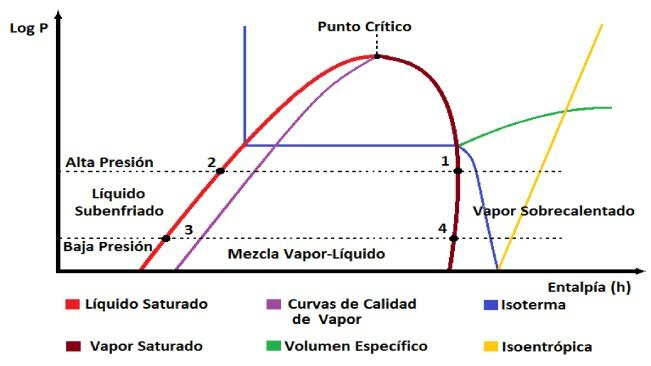
\includegraphics[width=.8\linewidth]{mollier}
	\end{figure}
	
		
		
		\part{Refrigerantes}
		\chapter{Refrigerantes}
\minitoc
\section{Refrigerantes y salmueras}
Un \textbf{refrigerante} es un medio (fluido) para la transferencia de calor que se utiliza en un sistema de refrigeración para absorber calor al evaporarse a temperatura y presión bajas, y ceder el calor al condensarse a temperatura y presión mayores.

La \textbf{salmuera} es un fluido utilizado como refrigerante secundario, transfiriendo el efecto frigorífico desde un circuito primario al espacio requerido.

\section{Nomenclatura}

Cada refrigerante se indica con un color.

El nombre de un refrigerante se representa mediante la letra R seguida de cuatro cifras que indican su composición química. 
\[\text{R}-\text{XXXX}\]
Cada una de estas cifras tiene un significado determinado (de izquierda a derecha):

\begin{enumerate}[label=$X_{\arabic*}$:]
	\item N° de enlaces de carbono no saturados —dobles o triples enlaces—.
	\item N° de átomos de carbono - 1.
	\item N° de átomos de hidrógeno + 1.
	\item N° de átomos de flúor.
\end{enumerate}

Además, en algunos casos, al nombre del refrigerante se le agrega una letra al final (por ejemplo, R-134a). Esta letra indica la \textbf{isomería} del compuesto. La \emph{isomería} es un fenómeno químico por el cual dos compuestos tienen la misma fórmula molecular, es decir, los mismos tipos y cantidades de átomos, pero diferente estructura o disposición espacial.

\section{Clasificación de los refrigerantes}

Los refrigerantes se pueden clasificar de distintas formas, según el criterio:

\begin{itemize}
	\item Según su \textbf{composición química}: orgánicos e inorgánicos, y dentro de estos se tienen los hidrocarburos y los halogenados.
	\item Según su \textbf{comportamiento}: puros, mezclas zeotrópicas o azeotrópicas.
\end{itemize}

\subsection{Clasificación por composición química}

\begin{itemize}
	\item \textbf{Inorgánicos}: no contienen átomos de carbono en su estructura química. Pertenecen a la familia de los refrigerantes R-700. Ejemplos: amoníaco (R-717), agua (R-718), dióxido de carbono (R-744). Su nomenclatura se escribe como \[\text{R-}700 + \text{peso molecular}\]
	\item \textbf{Hidrocarburos}: compuestos únicamente por carbono e hidrógeno. Son naturales y altamente inflamables. Ejemplos: R-290 (propano), R-600 (butano), R-600a (isobutano).
	\item \textbf{Halogenados}: derivados orgánicos que contienen flúor, cloro y/o bromo. Se subdividen en:
	\begin{itemize}
		\item \textbf{CFC (Cloro-Flúor-Carbono)}
		\item \textbf{HCFC (Hidrógeno-Cloro-Flúor-Carbono)}
		\item \textbf{HFC (Hidrógeno-Flúor-Carbono)}
	\end{itemize}
\end{itemize}

\subsection{Clasificación por comportamiento termodinámico}

\begin{itemize}
	\item \textbf{Refrigerantes puros}: formados por un solo compuesto. Cambian de fase a temperatura y presión constantes. Ejemplos: R-134a, R-290, R-744.
	\item \textbf{Mezclas zeotrópicas}: compuestas por dos o más refrigerantes que tienen diferentes puntos de ebullición, por lo tanto, cambian de fase con deslizamiento (\emph{glide}) de temperatura. Pertenecen a la familia R-400. Ejemplo: R-407C.
	\item \textbf{Mezclas azeotrópicas}: se comportan como un refrigerante puro en un punto específico de presión y temperatura. Cambian de fase sin deslizamiento. Pertenecen a la familia R-500. Ejemplo: R-507.
\end{itemize}

\subsection{Clasificación por peligrosidad}

Los refrigerantes se clasifican según su peligrosidad:
\begin{itemize}
	\item \textbf{Inflamabilidad}: números 1, 2, 3.
	\item \textbf{Toxicidad}: letras A y B.
\end{itemize}
\begin{figure}[h]
	\centering
	\caption{Clasificación de los refrigerantes según su peligrosidad, por ASHRAE Standard 34.}
	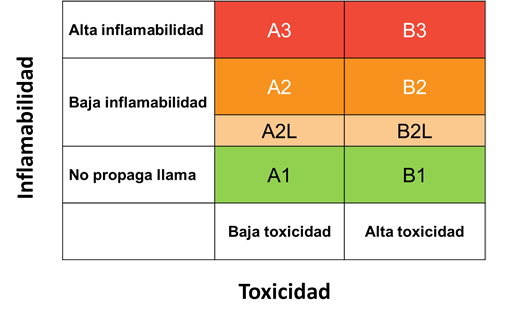
\includegraphics[width=0.5\linewidth]{refrigerantes/peligrosidad-refrigerantes}
\end{figure}

El triángulo Hidrógeno (H), Flúor (F), Cloro (Cl) es una herramienta visual para entender los compromisos y riesgos en la elección de refrigerantes.

\begin{itemize}
	\item Vértice superior: Hidrógeno (H). Aumenta la inflamabilidad de los refrigerantes.
	\item Vértice izquierdo: Cloro (Cl). Aumenta el ODP (Potencial de Destrucción del Ozono) y la toxicidad.
	\item Vértice derecho: Flúor (F). Disminuye la toxicidad, pero aumenta el GWP (Potencial de Calentamiento Global). Contribuye a la larga duración en la atmósfera.
\end{itemize}

\begin{figure}[H]
	\centering
	\caption{Triángulo H-F-Cl.}
	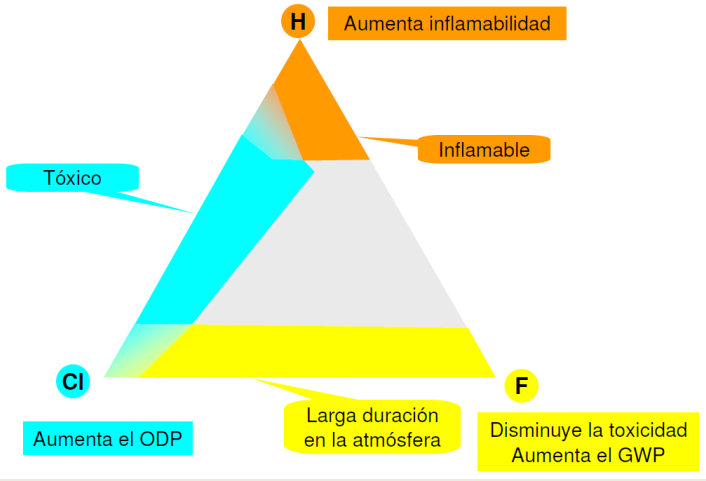
\includegraphics[width=0.6\linewidth]{refrigerantes/triangulo}
\end{figure}
\section{Código de colores}
Aunque fue muy usado durante años, AHRI (Air-Conditioning, Heating, and Refrigeration Institute) dejó de recomendar el uso del código de colores para cilindros a partir del 1 de enero de 2020 debido a las confusiones que ocasionaba, a las complejas mezclas que existen y a los errores que se podían cometer en el pintado.
\begin{figure}[H]
	\centering
	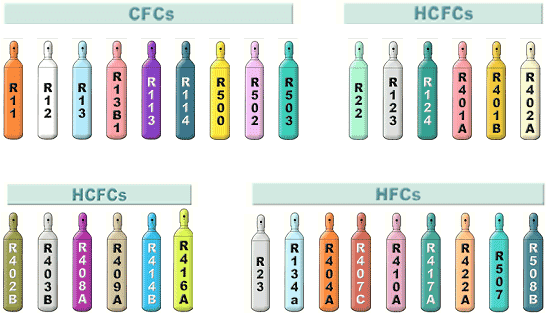
\includegraphics[width=\linewidth]{refrigerantes/codigo-colores}
	\caption{Código de colores para los cilindros de refrigerantes.}
\end{figure}
\section{Requisitos de los refrigerantes}

\begin{itemize}
	\item \textbf{Presiones}: la presión de condensación debe estar muy por debajo de la crítica, debido a bajos calores latentes, además, no tiene una distinción clara entre fase líquida y gaseosa. La presión de evaporación debe estar por encima de la atmosférica, para que no haya filtraciones e ingrese aire exterior.
	\item \textbf{Calor latente de vaporización}: es el calor que absorberá. Representado por una horizontal en el diagrama de Mollier.
	\item \textbf{Calor latente de condensación}: es el calor que cederá al exterior. Representado por una horizontal en el diagrama de Mollier, por encima del de vaporización.
	\item \textbf{Temperatura}: no debe ser excesivamente alta para evitar la descomposición del lubricante —y daños en el compresor—.
	\item \textbf{Punto de congelación}: debe ser bajo, por obvias razones creo yo. Para que no se congele dentro del circuito y se tranque como la caca en el inodoro.
	\item \textbf{Exponente isoentrópico}: debe ser reducido. A mayor exponente, mayor trabajo de compresión necesario. En el diagrama ph se representa como una recta inclinada en la compresión: más inclinada, más energía requiere para comprimirse.
	\item \textbf{Peligrosidad}: no debe ser tóxico ni dañino para personas, componentes del sistema, ni con el medioambiente.
	\item \textbf{Accesibilidad}: debe estar disponible y ser de bajo costo —aguante el capitalismo—.
\end{itemize}

\subsection{Potencial de Calentamiento Global (GWP)}
El GWP (Global Warming Potential) indica cuánto contribuye un gas al calentamiento global comparado con el dióxido de carbono.

\subsection{Potencial de Destrucción del Ozono (ODP)}
El ODP (Ozone Destruction Potential) mide la capacidad de una sustancia para destruir la capa de ozono.



\section{Resumen}

El cuadro presenta un resumen de los refrigerantes más comunes, clasificados por colores según su nivel de uso actual: en rojo, los que están en desuso; en naranja, los que se encuentran en proceso de ser reemplazados; y en verde, los que se utilizan actualmente y continuarán en uso a largo plazo.
\begin{figure}[h]
	\centering
	\caption{Clasificación de los refrigerantes.}
	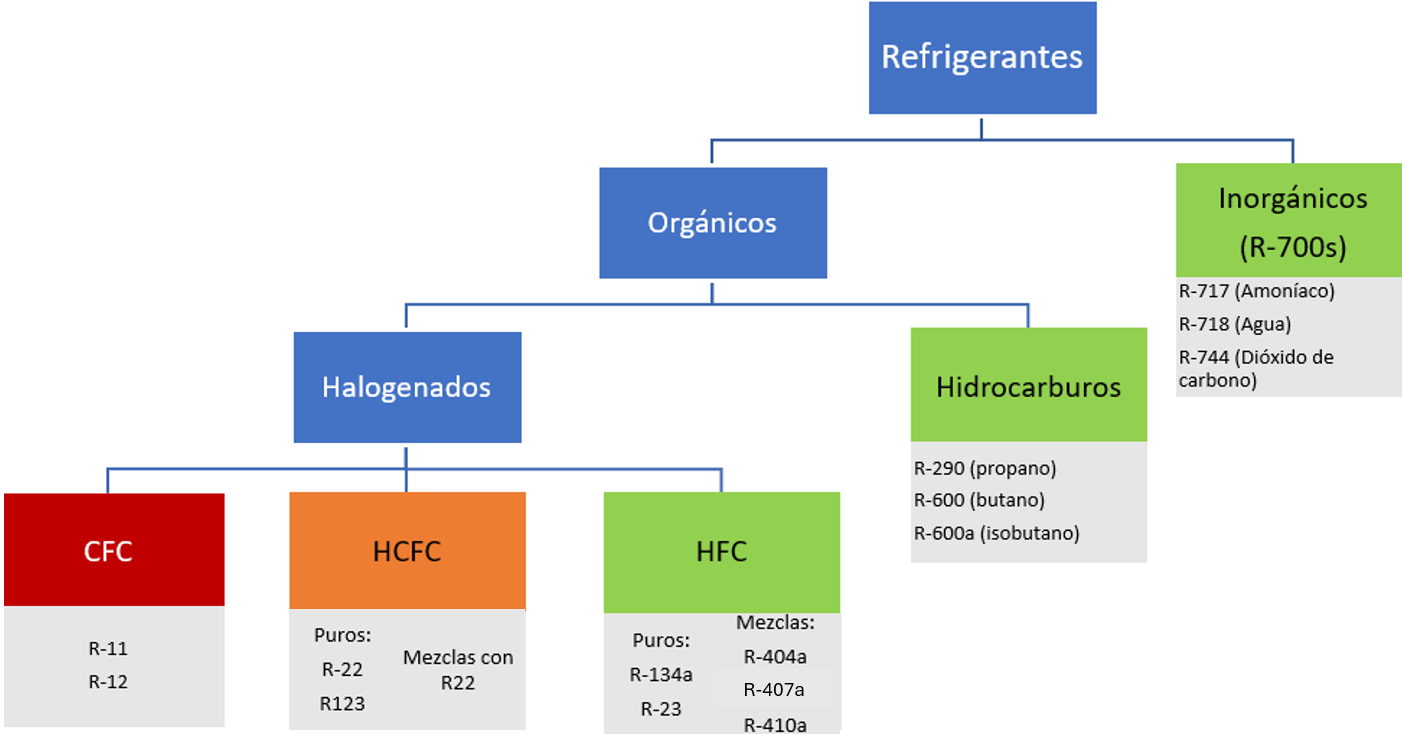
\includegraphics[width=\linewidth]{refrigerantes/resumen}
\end{figure}
		
		\part{Refrigeración por Compresión}
		% Unidad 3
\chapter{Refrigeración por compresión}
\minitoc

	La refrigeración por compresión es el método más utilizado en aplicaciones domésticas, comerciales e industriales para la conservación de alimentos, el aire acondicionado y procesos industriales que requieren temperaturas controladas. Este sistema opera mediante un ciclo termodinámico cerrado, en el que un refrigerante cambia de fase para absorber y ceder calor, permitiendo la transferencia de energía térmica de una zona fría a una más caliente.
	
	El ciclo básico consta de cuatro procesos fundamentales:
	
	\begin{itemize}
		\item Compresión: El refrigerante en estado gaseoso es comprimido, aumentando su presión y temperatura.
		
		\item Condensación: El gas comprimido cede calor al ambiente y se condensa en estado líquido.

		\item Expansión: El líquido refrigerante pasa por una válvula de expansión, reduciendo su presión y temperatura.
		
		\item Evaporación: En el evaporador, el refrigerante absorbe calor del espacio refrigerado y se evapora, repitiendo el ciclo.
	\end{itemize}

%Temas a desarrollar

	\section{Tipos de sistemas de refrigeración por compresión}
	
	Se pueden clasificar según el número de etapas, el tipo de compresor, el método de condensación, y la distribución del refrigerante en el evaporador.
	
	\subsection{Según la distribución del refrigerante en el evaporador}
	
	Los principales tipos de sistemas de refrigeración por compresión clasificados según el tipo de alimentación o distribución del refrigerante en el evaporador son:
	\begin{itemize}
		\item Sistema de expansión directa.
		\item Sistema inundado o de refrigeración por líquido inundado.
		\item \ver{Lo que sigue hay que buscarlo en algún libro o algún lugar más verídico que chatgpt}
		\item Sistema de expansión seca. Caso particular de la expansión directa.
		\item Sistema de película descendente
		\item Sistema de circulación forzada.
		\item Sistema con recirculación por bombeo.
	\end{itemize}
	
	\section{Ciclo de refrigeración por compresión}

\subsection{Elementos fundamentales}

Los sistemas de refrigeranción por compresión constan, básicamente, de cuatro elementos que consideramos fundamentales a través de los cuales circula un fluido refrigerante.

Estos elementos son:

\begin{enumerate}
	\item Compresor
	\item Condensador
	\item Dispositivo de expansión
	\item Evaporador
\end{enumerate}

\begin{figure}[h]
	\centering
	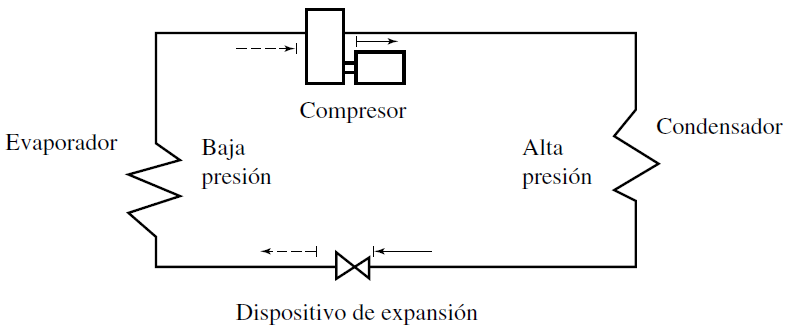
\includegraphics[width=\textwidth]{figuras/elementos fundamentales.png}
	\caption{Elementos fundamentales de un sistema de refrigeración}
	\label{fig:elementos_fundamentales}
\end{figure}


\subsubsection{Funciones principales}

La función de cada uno de ellos es la siguiente:

\textbf{Compresor:}

Aspira el fluido refrigerante a la presión de baja establecida y lo comprime elevando su presión y temperatura hasta unos valores tales que se pueda efectuar la condensación. La descarga la efectua en el condensador.

\textbf{Condensador:}

Es el elemento de la instalación que se encarga de pasar el estado de vapor del fluido refrigerante a estado líquido. El fluido refrigerante entra en el condensador en estado de gas (vapor recalentado) y sale en estado líquido a la temperatura que se condensó o incluso a una temperatura menor si se produce subenfriamiento.

\textbf{Dispositivo de expansión:}

Hace que el fluido, que entra en estado líquido, sufra una caída de presión (y temperatura) hasta la necesaria en el evaporador. También controla la cantidad de fluido refrigerante que debe entrar en el evaporador.

\textbf{Evaporador:}

Se encarga de enfriar o acondicionar la cámara. Puede estar dentro o fuera de la misma. Su misión es que el fluido refrigerante, que entra a baja presión y temperatura, efectúe el enfriamiento.\\
Es el elemento de la instalación donde el fluido refrigerante se evapora, tomando calor del exterior del evaporador debido a la diferencia de temperaturas.

\subsubsection{Fluido refrigerante}

El fluido refrigerante está sometido a cambios de estado a lo largo del circuito:

\begin{itemize}
	\item En el compresor entra en estado de gas, a baja presión y temperatura, y sale con presión y temperatura más altas (recalentado), que es como entra en el condensador.
	\item Del condensador sale estado líquido y entra dispositivo de expansión.
	\item Del dispositivo de expansión sale en forma de mezcla de líquido y gas (expansión), a baja presión y temperatura, y entra en el evaporador.
	\item Del evaporador sale en estado de gas, a baja presión y temperatura, de donde es aspirado por el compresor, y se inicia el nuevo ciclo.
\end{itemize}

Como sabemos, \textit{al aumentar la presión de un fluido se eleva su punto de ebullición, y al disminuir la presión, también disminuye su punto de ebullición.} Esta es una de las claves de la refrigeración.

\subsection{Alta y baja presión}

Debemos diferenciar la parte del circuito que está sometida a una presión alta y la que se encuentra a baja presión (\autoref{fig:elementos_fundamentales}).

\textit{La parte correspondiente a la alta presión está comprendida entre la descarga del compresor y la entrada del dispositivo de expansión.}

Hay que resaltar que la temperatura del fluido refrigerante no es la misma en todo ese tramo:

\begin{itemize}
	\item Entre la salida del compresor y la entrada del condensor el fluido está en estado de gas (gas recalentado).
	\item Se condensa a una temperatura menor y s desde el vale del condensador a esa misma temperatura o menor si se subenfría, con lo cual, la temperaturadel fluido a la entrada del dispositivo de expansión puede ser igual o menor que la de condensación.
\end{itemize}

\textit{La parte que corresponde a la baja presión, es la comprendida entre la salida del dispositivo de expansión y la entrada del compresor.}

La instalación dispone del manoómetro de baja presión para conocer su valor en cada momento. En este tramo, también la temperatura varía (aumenta) desde el evaporador hasta la entrada del compresor.

\subsection{Elementos de seguridad y control}

La \autoref{fig:elementos_seguridad_y_control} representa los cuatro elementos fundamentales para el estudio de sus principales características a los que se añaden los elementos de seguridad y control.

\begin{figure}[H]
	\centering
	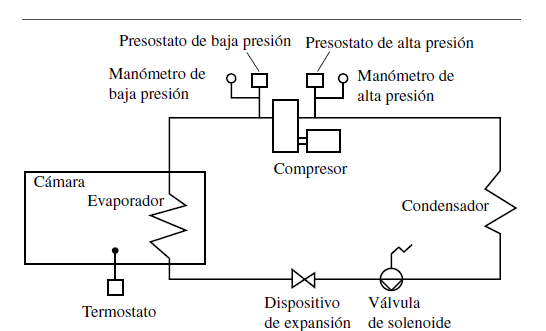
\includegraphics[width=\textwidth]{Elementos_seguridad_y_control.png}
	\caption{Elementos fundamentales de un circuito frigorífico en los que se añaden los dispositivos de seguridad y control.}
	\label{fig:elementos_seguridad_y_control}
\end{figure}

\subsubsection{Presostatos}

Son unos aparatos que, activados por presión, tienen la función de abrir o cerrar un circuito mediante uno o varios contactos normalmente ya sean abiertos o cerrados. De manera práctica, se puede decir que son unos interruptores eléctricos que funcionan por presión. Pueden ser:

\begin{enumerate}
	[a.]
	\item Presostatos de alta presión 
	
	Se conecten a la descarga del compresor, y su función es impedir que en la zona de alta presión, se alcancen valores que afecten al rendimiento de la instalación o a la propia seguridad de las personas. Se regulan a una determinada presión, y cuando la instalación alcanza ese valor, entonces el presostato para el compresor.
	\item Presostatos de baja presión
	
	Se conectan a la aspiración del compresor, y función es evitar que la presión, en la zona baja, pueda ``caer'' por debajo de la presión atmosférica y evitar también que la presión descienda por debajo de la normal de funcionamiento, ya que afectaría al rendimiento. De hecho, su regulación debe estar \textit{siempre} por encima de la presión atmosférica. Cuando la presión descienda hasta la correspondiente al valor de regulación, el presostato parará el compresor. 
\end{enumerate}

Los presostatos de alta y baja presión no tienen que instalarse necesariamente por separado, ya que también se puede instalar los dos formando un solo elemento, llamado \textit{presostato combinado}, tal como se representa en la \autoref{fig:Presostato combinado}.

\begin{figure}[H]
	\centering
	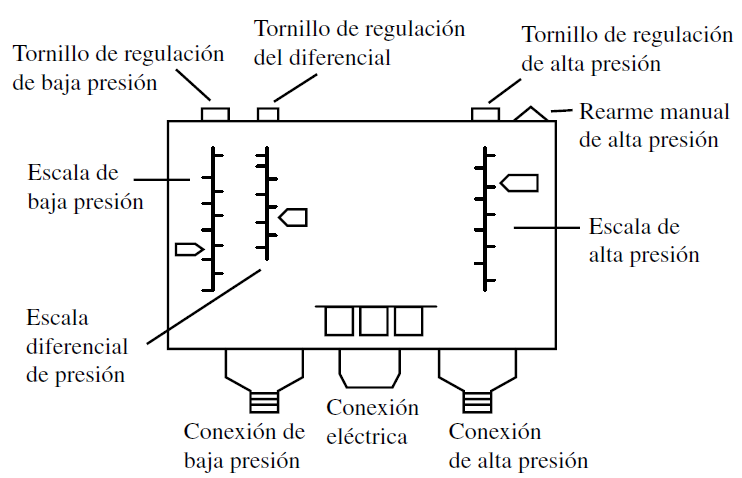
\includegraphics[width=\textwidth]{figuras/presostato combinado.png}
	\caption{Presostato combinado}
	\label{fig:Presostato combinado}
\end{figure}

\subsubsection{Termostato}

Es el elemento que controla la temperatura de la cámara. Abre o cierra un contacto conectado a un circuito eléctrico cuando alcanza la temperatura de regulación. Se puede decir que es un interruptor o conmutador eléctrico que funciona por temperatura.

El termostato con depósito de gas, se basa en que éste sufre variaciones de presión en relación a la temperatura que rodea al depósito que lo contiene. Si una de las paredes del depósitoes de membrana, sufrirá deformaciones a consecuencia de esos cambios de temperatura. Si además actúa sobre unos contactos, bien sea directa o inderectamente, los abrirá o cerrará de acuerdo a la regulación establecida. 

Como los presostatos, disponen de un diferencial (diferencia entre las temperaturas de arranque y de paro) que puede ser fijo o variable. Por lo general suele ser de $\pm 3$.

\textbf{Ejemplo de aplicación}

Queremos mantener una temperatura de -20 \textcelsius en la cámara y el diferencial establecido es de $\pm 3$ \textcelsius.

Ello quiere decir que la instalción se parará cuando la temperatura alcance los -23 \textcelsius, pues el termostato, en ese momento, cerrará la válvula de solenoide. Debido a la transmisión de calor, la temperatura en el interior de la cámara aumentará hasta alcanzar los -17 \textcelsius y entonces el termostato abrirá la válvula de la solenoide, y se pondrá de nuevo en funcionamiento el compresor.

\subsubsection{Válvula de solenoide (o electroválvula)}

Aunque no es un elemento de regulación ni de control, debemos comentar sus principales características para poder enterder mejor el siguiente apartado.

Su funcionamiento es de todo o nada, no es de regulación proporcional. Cuando está activada por el campo magnético, levanta el vástago de la válvula y deja pasar el fluido. Cuando se desactiva, cesa la imanación (no hay campo magnético), el vástago de la válvula cae y corta el paso del fluido refrigerante.

Va conectada en serie con el termostato, por decirlo de una mnera práctica; el termostato deja pasar o corta la corriente eléctrica a la bobina, con lo cual la válvula se abre o cierra, según las necesidades térmicas.


\begin{figure}[H]
	\centering
	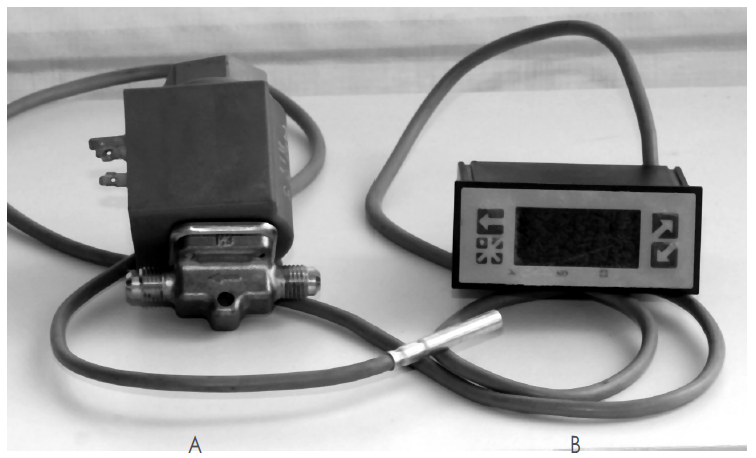
\includegraphics[width=\textwidth]{figuras/solenoide y termometro.png}
	\caption{A: Válvula de solenoide. B:Termostato electrónico}
	\label{fig:solenoide y termostato}
\end{figure}

\subsubsection{Presostato diferencial de aceite}

Es un elemento de seguridad; de hecho es un interruptor de seguridad (\autoref{fig:Presostato diferencial de aceite}). PRotege al compresor contra una presión de aceite demasiado baja. Se conecta a la aspiración y a la descarga de la bomba de lubricación.

\begin{figure}[H]
	\centering
	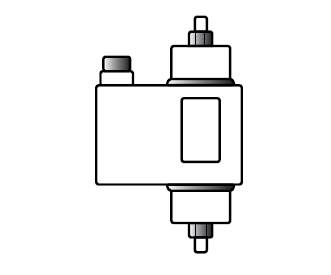
\includegraphics[width=6cm, height=6cm]{figuras/Presostato diferencial de aceite.png}
	\caption{Presostato diferencial de aceite}
	\label{fig:Presostato diferencial de aceite}
\end{figure}

\subsection{Elementos complementarios}
Una instalación podría trabajar con los elementos anteriormente citados, pero, evidentemente, necesita de otros elementos complementarios para que el ciclo de trabajo se pueda efectuar con el mayor rendimiento posible. 

En el siguiente esquema (\autoref{fig:Instalacion con elementos complementarios} se representan los más importantes y su disposición en las instalaciones.)

\begin{figure}[H]
	\centering
	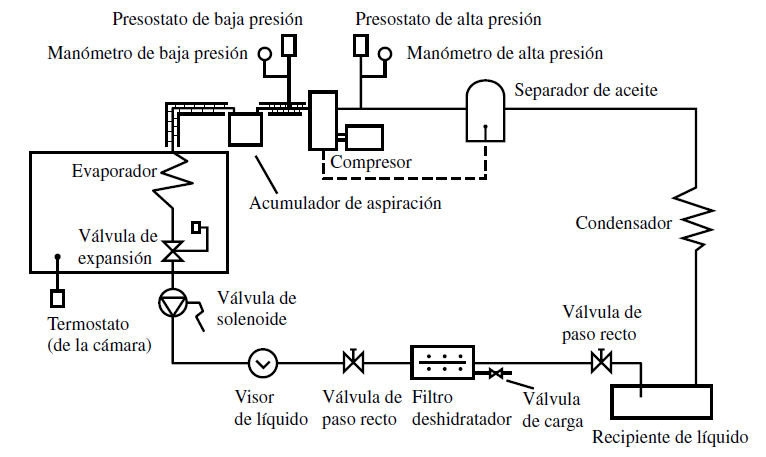
\includegraphics[width=\textwidth]{figuras/Instalación con elementos complementarios.png}
	\caption{Instalación de los elementos fundamentales, de seguridad y control, y complementarios}
	\label{fig:Instalacion con elementos complementarios}
\end{figure}

\subsubsection{Resistencia calefactora (del cárter)}

Cuando las temperaturas que rodean al compresor (temperatura ambiente) son muy bajas, en los tiempos de parada del compresor puede ocurrir que el fluido refrigerante depositado en el cárter se condense, por lo que en el momento del arranque se produce una vaporización rápida del fluido que conlleva un arrastre de aceite.

También la baja temperatura ambiente afecta a la viscosidad del aceite, ya que si es muy baja, ésta aumenta las resistencias a vencer en el arranque. Para evitar estas circunstancias se instalan en el cárter unas peque\~{n}a resistencias eléctricas que lo mantienen a cierta temperatura, de tal manera que cuando para el compresor, entran en funcionamiento.

\subsubsection{Separador de aceite}

Se instala en la tubería de descarga, después del compresor. El fluido refrigerante sale del compresor mezclado con el aceite de lubricación y éste debe retornar al cárter principalmente por dos razones:

\begin{enumerate}
	[1.]
	\item  porque el nivel de aceite del cárter iría disminuyendo y
	\item porque el aceite, cuando llegue al circuito de baja presión, podría tener problemas de retorno (deja de ser miscible y crea problemas en los evaporadores, por ejemplo de transmisión o taponamientos)
\end{enumerate}

Los hay de varios tipos. Por ejemplo los que aprovechan la fuerza centrífuga de la descarga del compresor para efectuar la separación (Figura \ref{fig:Separador de aceite}) o bien la caída de velocidad a la entrada del separador para efectuar la separación.

%     LO DEJO COMENTADO PORQUE DESP TE LO QUIERO MOSTRAR A VER SI VOS SABES QUE PASA
%	Si recortamos las imágenes como para que quede centrado el objeto, mejor :)
\begin{wrapfigure}{r}{0.4\linewidth}
	\centering
	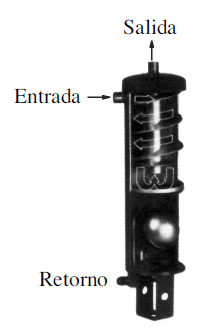
\includegraphics[width=.5\linewidth]{figuras/separador de aceite.png}
	\caption{Separador de aceite}
	\label{fig:Separador de aceite}
\end{wrapfigure}  

El aceite se va decantando en el fondo del separador hasta alcanzar un nivel tal que el regulador, por ejemplo un flotador de nivel, lo detecta y abre el paso de retorno hacia el cárter.

Una representación del retorno de aceite se puede observar en la \autoref{fig:Línea de retorno de aceite}.


Cuando el nivel de aceite en el interior del separador alcanza el nivel estipulado, el regulador de nivel abre la electroválvula y el aceite retorna al cárter. El aceite retorna porque la presión en el interior del separador (presión de alta) es superior a la presión reinante en el cárter.

No tienen una eficacia del 100\%, pero es bueno que una pequeña cantidad de aceite circule por la instalación ya que mantiene engrasados elementos como válvulas, electroválvulas, etc.

\begin{figure}[h]
	\centering
	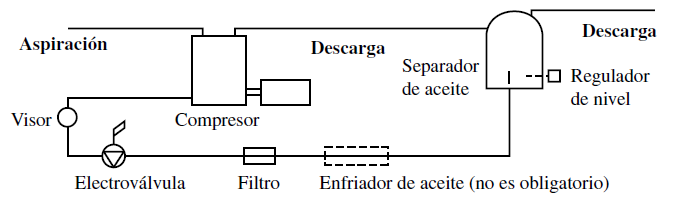
\includegraphics[width=.9\linewidth]{figuras/Linea de retorno de aceite.png}
	\caption{Línea de retorno de aceite}
	\label{fig:Línea de retorno de aceite}
\end{figure}

\subsubsection{Recipiente de líquido}

Se coloca a la salida del condensador, aunque los hay del tipo condensador-recipiente que forman un solo elemento.

El líquido que sale del condensador no va directamente al evaporador, salvo si se utilizan tubos capolares, sino que se ``almacena'' en el recipiente. Mantiene una reserva de líquido para restituirlo según la demanda. Los hay horizontales (\autoref{fig:Recipiente de líquido horizontal}) y (\autoref{fig:Recipiente de líquido vertical}) verticales.

Su capacidad varía con las características de la instalación; si se trata de una con varios evaporadores, su capacidad será por lo menos 1,25 veces la capacidad del evaporador mayor.

\begin{figure}[H]
	\centering
	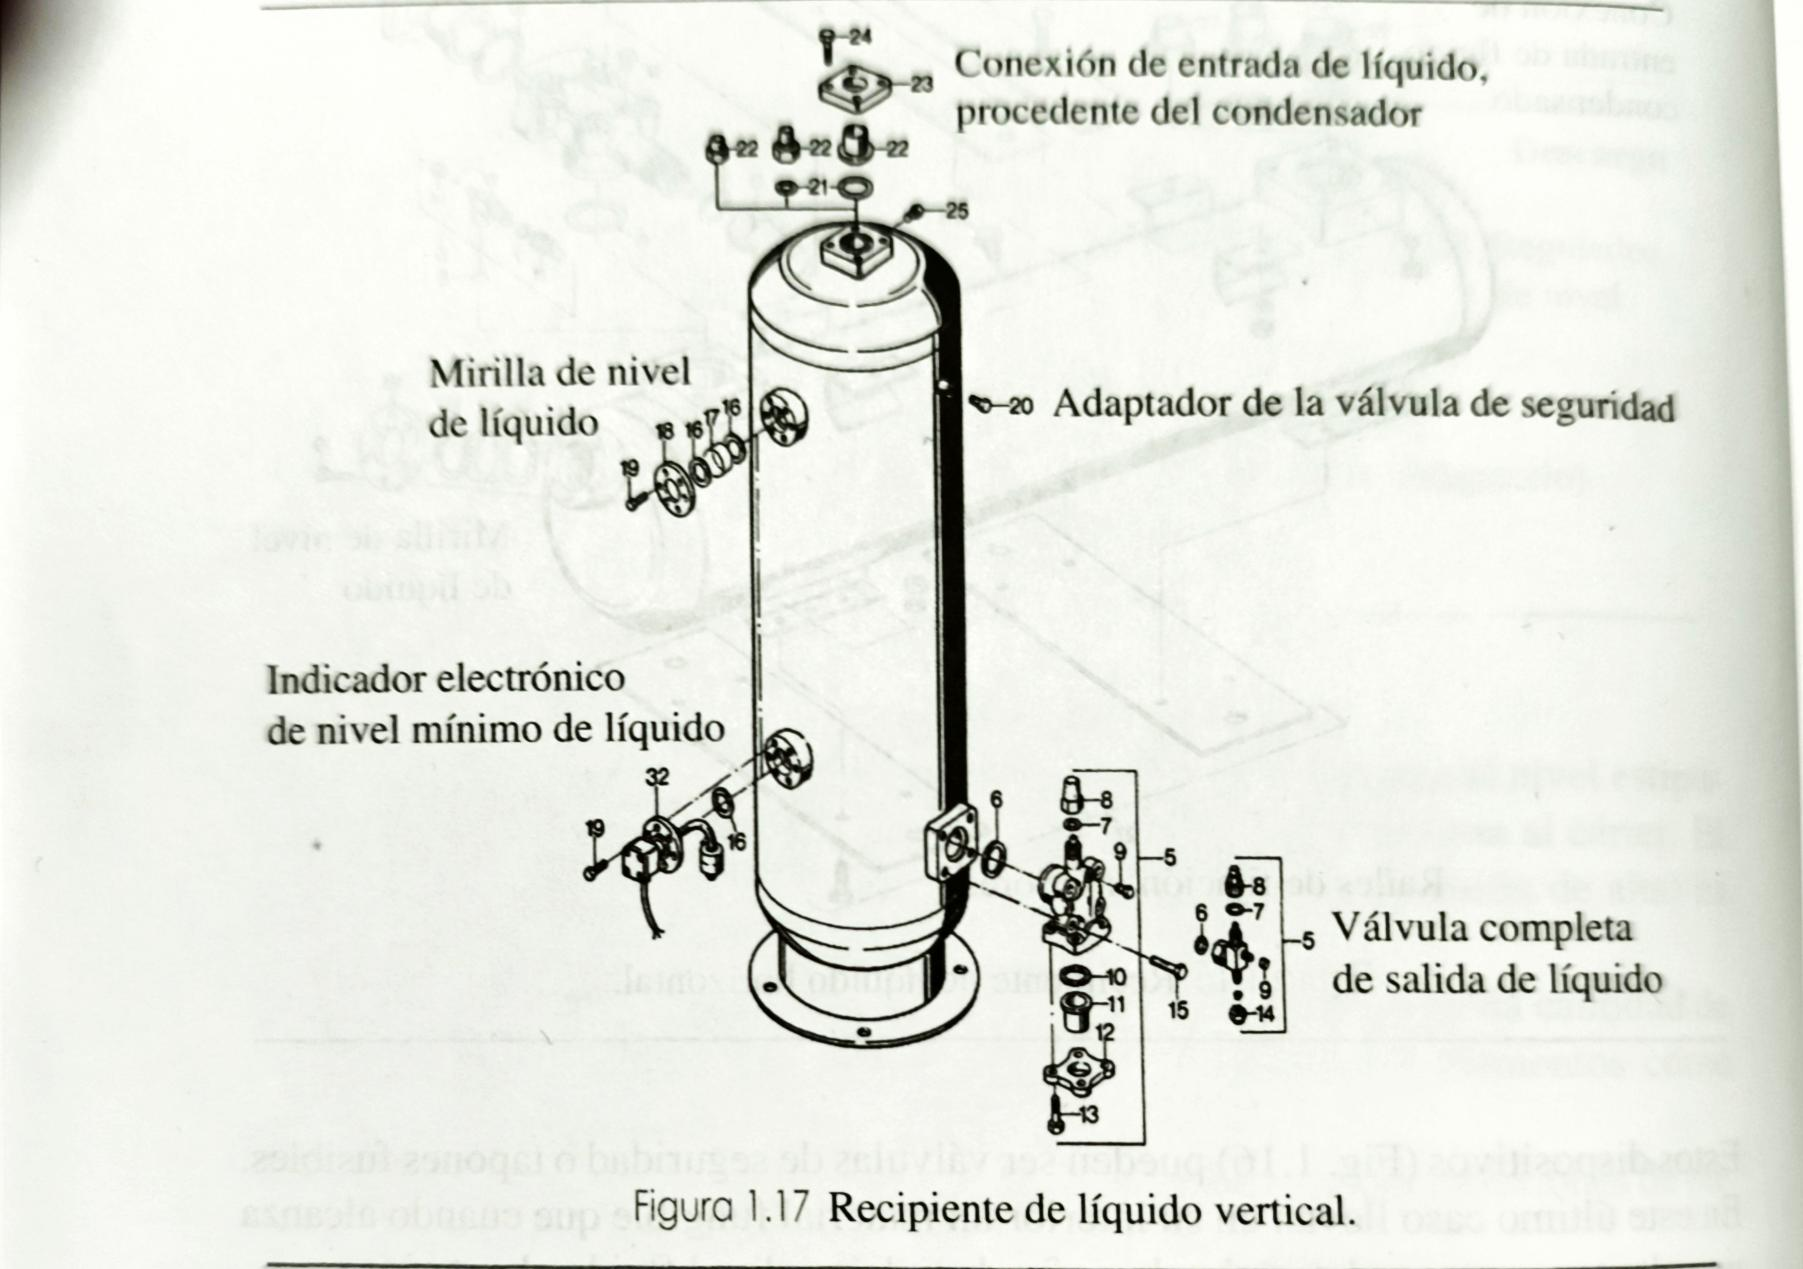
\includegraphics[width=0.7\textwidth]{figuras/recipiente vertical.jpg}
	\caption{Recipiente de líquido vertical}
	\label{fig:Recipiente de líquido vertical}
\end{figure}

\begin{figure}[H]
	\centering
	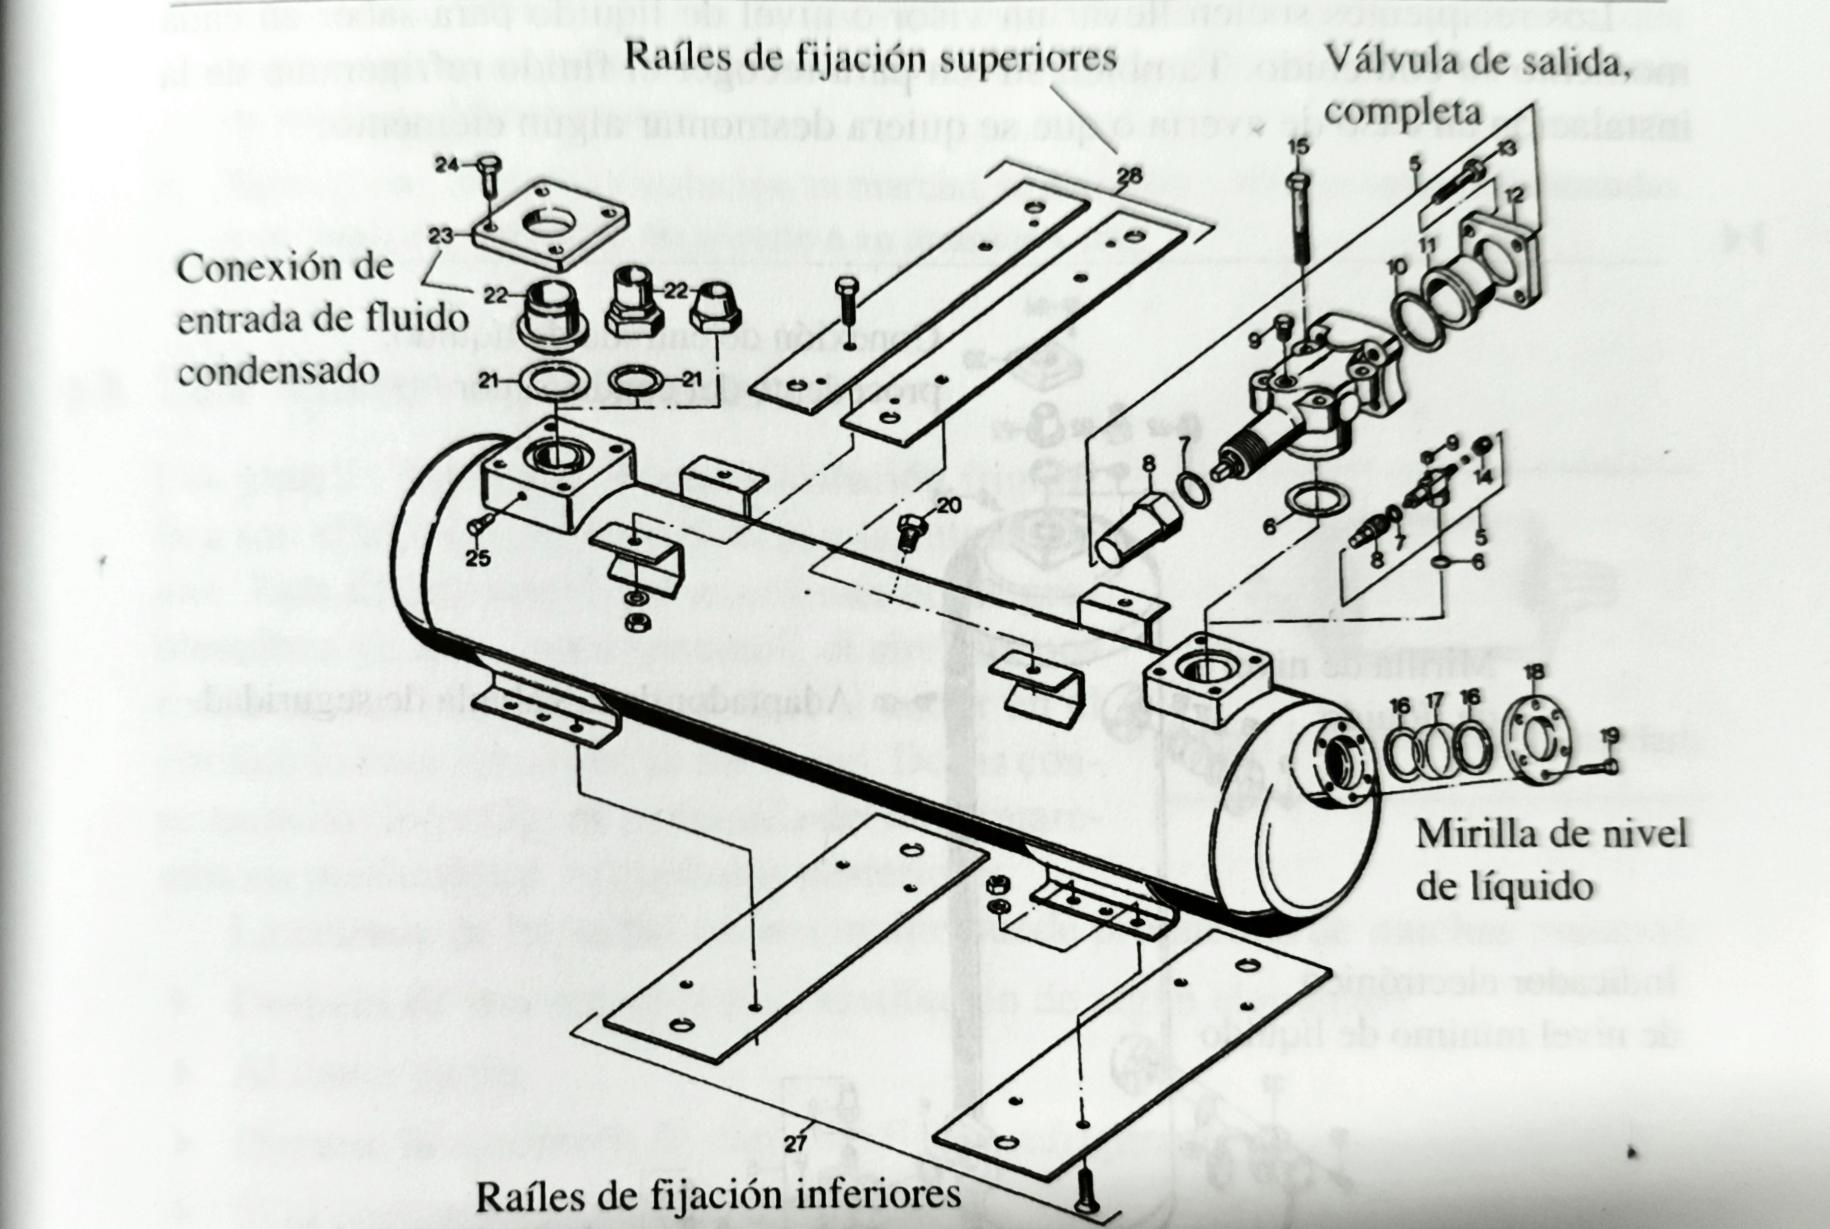
\includegraphics[width=0.7\textwidth]{figuras/recipiente horizontal.jpg}
	\caption{Recipiente de líquido horizontal}
	\label{fig:Recipiente de líquido horizontal}
\end{figure}

Al ser un recipiente de alta presión, debe llevar sus dispositivos de seguridad para evitar que se almacenen presiones peligrosas. También suelen llevar un visor o nivel de líquido para saber en cada momento su contenido.

\subsubsection{Filtros de humedad}

Los grandes enemigos de una instalación frigorífica son el temido golpe de líquido y la entrada de aire. Esta última implica a su vez la doble problemática, como sabemos, el aire que nos rodea es aire húmedo, con lo cual al entrar en el circuito lo hace junto con su humedad.

La entrada de humedad en un circuito puede producirse de muchas maneras:

\begin{itemize}
	\item Después de una reparación (o sustitución de un elemento)
	\item Al meter aceiteDurante la operación de carga de un fluido refrigerante
	\item Si el compresor aspira del aire ambiente
\end{itemize}

La humedad puede ocasionar serios problemas tales como bloquear los dispositivos de expansión (congelación de esas gotas del aire húmedo) o bien producir problemas en los compresores herméticos o semiherméticos, oxidaciones, etc. Para evitar la humedad en los circuitos se instalan unos filtros de humedad también llamados deshidratadores. Contienen un agente desecante que puede ser:

\begin{itemize}
	\item Silicagel
	\item Tamices moleculares
	\item Alúmina activada 
	\item Óxido de aluminio, muy empleado con los nuevos fluidos refrigerantes
\end{itemize}

También existen los denominados núcleo sólido, que son una mezcla de silicagel, tamices moleculares y óxido de aluminio.

Los filtros de humedad además de su función deshidratadora, retienen impurezas (partículas sólidas). 

A la hora de instalarse se deben seguir las intrucciones y el sentido de instalación indicado por el fabricante, si este sentido además es vertical desendente se aumentara el rendimiento del dispositivo.

\textit{La eficacia del agente desecante aumenta cuanto menor sea la temperatura del líquido a la entrada del filtro.} Supongamos, por ejemplo, una instalación con condensador por aire. En verano, al aumentar la temperatura ambiente, también aumenta la temperatura de condensación y por lo tanto la del líquido, lo que influye en la eficacia del agente deshidratador y puede provocar congelación en las válvulas de expansión. Por ello si se debiera instalar un intercambiador de calor, el filtro se montaría después.

\subsubsection{Visor}

De manera práctica diremos que es una ``ventana'' que tenemos en el circuito. A través de él deberíamos ver el fluido en estado líquido 100\% (saturado). Si, por ejemplo vemos burbujas, podría indicarnos que hace falta fluido refrigerante (poca carga, bien sea porque de origen no tiene la adecuada o por fugar posteriores) o bien, si hay burbujar y está frío, puede ser porque un estrangulamiento origina un expansión antes de llegar al visor. También nos indica si hay humedad en el circuit, ya que contiene una sal química higroscópica que reacciona con la humedad y cambia de color (no todos lo tienen).

\subsubsection{Acumulador de aspiración}

Es un elemento que se instala en el lado de baja presión, antes del compresor. Su función consiste en evitar que llegue el fluido en estado líquido al compresor. Es un recipiente metálico, que por lo general suele llevar un tubo de entrada y otro de salida. Evidentemente,\textit{el tubo de entrada se conecta a la tubería que viene del evaporador, y el de salida a la que va al compresor.}

No hay que confundir el acumulador de aspiración con el \textit{separador de líquido}, ya que éste es un elemento de las instaciones de régimen inundado y está perfectamente aislado, pues contiene el fluido expansionado a baja presión y temperatura.

\subsubsection{Intercambiador de calor}

Algunas instalaciones llevan intercambiadores de calor a contracorriente líquido-vapor de aspiración. Es decir, se produce intercambio de calor entre el líquido refrigerante procedente del recipiente y el vapor de salida del evaporador.

\begin{figure}[H]
	\centering
	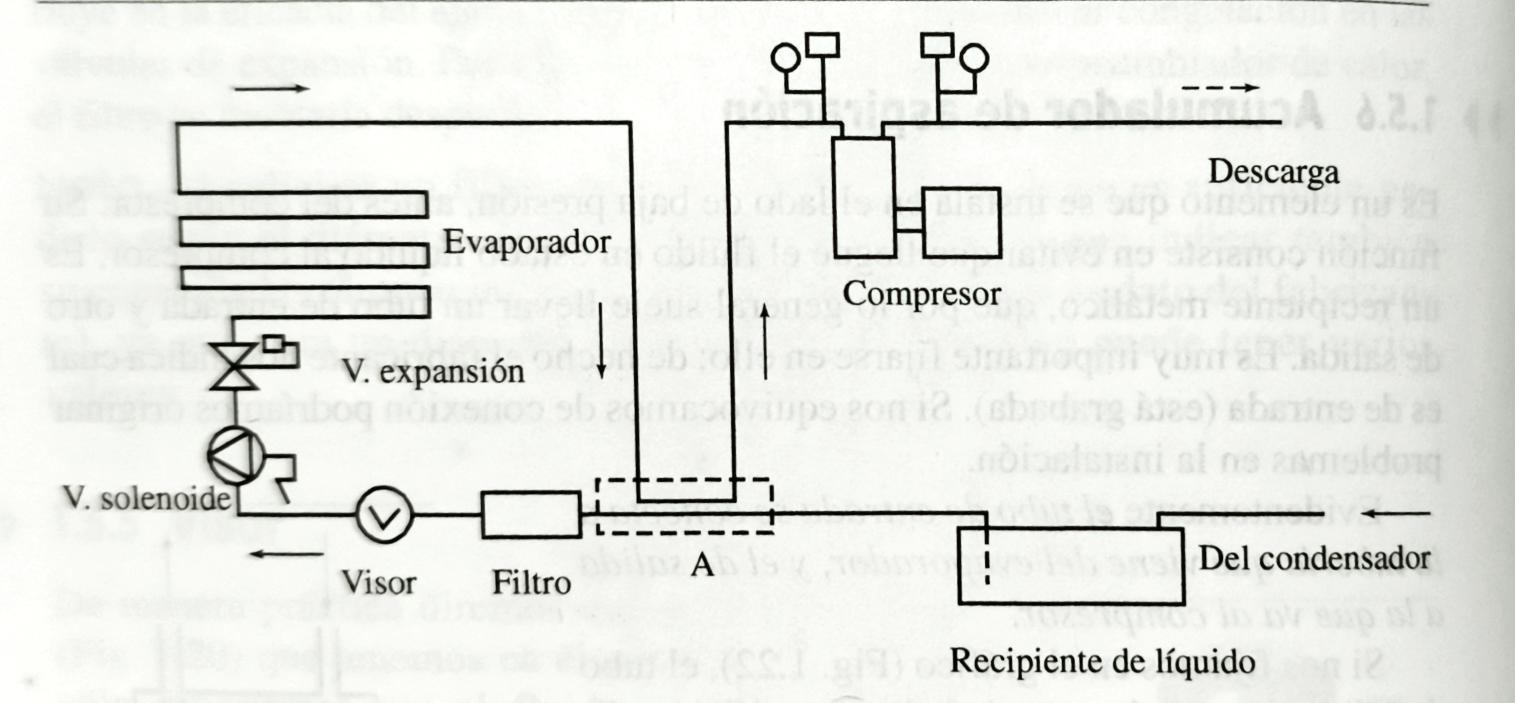
\includegraphics[width=\textwidth]{figuras/instalación con intercambiador.jpg}
	\caption{Instalación con intercambiador de calor}
	\label{fig:Instalación con intercambiador de calor}
\end{figure}

Al ser estos elementos intercambiadores de calor, tienen doble lectura:

\begin{enumerate}[a.]
	\item La del vapor frío de la aspiración que subenfría el líquido que va al dispositivo de expansión y aumenta el rendimiento dado que la temperatura con que entra el líquido en dicho dispositivo es menor (válvula de expansión en la \autoref{fig:Instalación con intercambiador de calor}).
	\item La temperatura del líquido que al estar en contacto con la tubería de salida del evaporador, vaporiza las posibles gotas de líquido que vayan al compresor, es decir evita que llegue líquido al compresor.
\end{enumerate}

 % Acá se habla del circuito básico y típico, los componentes que lleva y entre otras cosas
	
	\section{Diagramas de ciclos de refrigeración}\label{sec:1}

	En esta sección se utiliza como fuente principal el libro \emph{Principios de Refrigeración} de \cite[Capítulos 6 y 7]{dossat2004refrigeracion}.
	
	Los diagramas que con frecuencia se usan en el análisis del ciclo de refrigeración son los de \textit{presión-entalpia (ph)} y \textit{temperatura-entropía (Ts)}.
	
	%	Agregar gráfica de los diagramas ph y Ts para mostrar las regiones
	
	\subsection{Ciclo de refrigeración teórico} \label{sec:ciclo-teorico}
	
	%	Desarrollo del diagrama para un ciclo teórico
	
		El ciclo teórico es un ciclo de refrigeración saturado simple en el cual se supone que el vapor refrigerante que sale del evaporador y entra al compresor es vapor saturado a la temperatura y presión vaporizante, y el líquido refrigerante que sale del condensador y llega a la válvula de expansión es un líquido saturado a la temperatura y presión condensante. Además, se desprecian las pérdidas en las tuberías y en los accesorios.

		% Mencionar la disposición de los elementos y agregar la fig 7-5 del libro
		
		\begin{figure}[h]
			\centering
			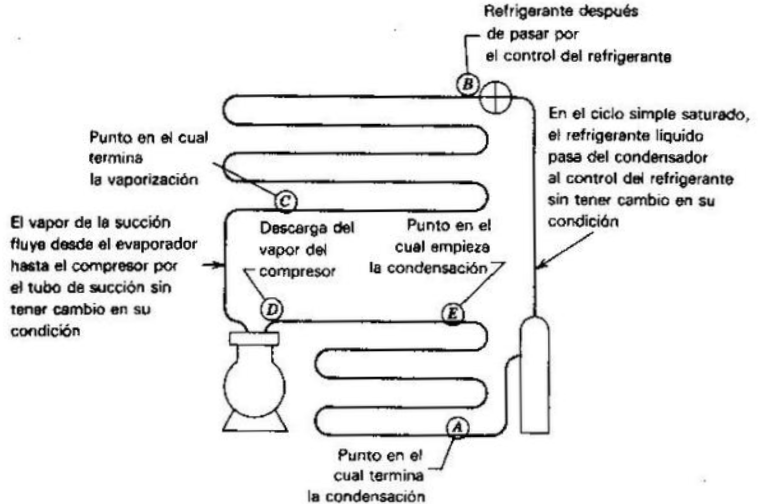
\includegraphics[width=.7\linewidth]{ciclo-saturado-simple}
			\caption{Diagrama de flujo de un ciclo saturado simple.}
			\label{fig:ciclo-teorico}
		\end{figure}
		
		\begin{figure}[h]
			\centering
			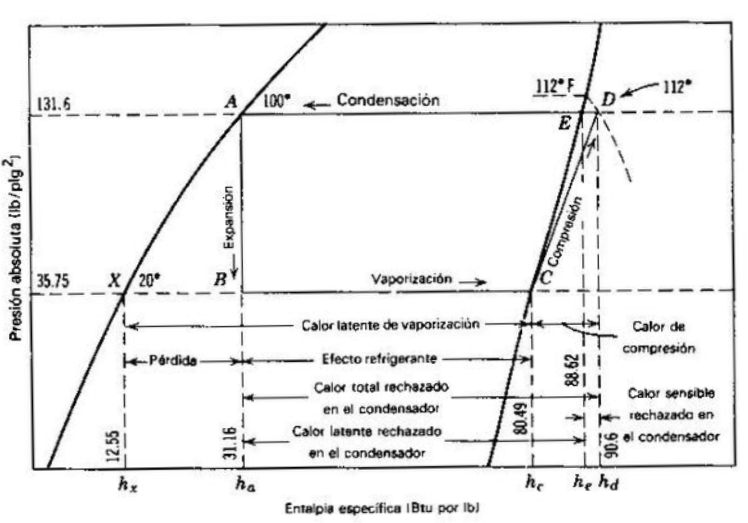
\includegraphics[width=.7\linewidth]{diagrama-ciclo-saturado-simple}
			\caption{Diagrama de flujo de un ciclo saturado simple.}
			\label{fig:diagrama-teorico}
		\end{figure}
		
		En el diagrama de la \autoref{fig:ciclo-teorico} se tiene el trazo de un ciclo saturado simple, y en la \autoref{fig:diagrama-teorico} se muestra un diagrama presión-entalpía de dicho ciclo, en el cual se observan cuatro transformaciones o procesos:
		
		\begin{itemize}
			\item Expansión.
			\item Evaporación.
			\item Compresión.
			\item Expansión.
		\end{itemize}
		
		\subsubsection{Proceso de expansión} El proceso de expansión es representado en el diagrama por el trazo $A-B$. Es un estrangulamiento tipo expansión adiabática y sucede en la válvula de expansión cuando la presión del líquido refrigerante es reducida desde la presión en el condensador a la presión en el evaporador. La temperatura del líquido que llega a la válvula de expansión A siempre es bastante mayor que la temperatura en el evaporador B y ésta deberá primero reducirse hasta dicha temperatura antes de que el líquido pueda vaporizarse en el evaporador.
			
			
			 
			En este ciclo teórico no hay ningún cambio en las propiedades del líquido refrigerante a medida que éste fluye a través de la línea de líquido desde el condensador a la válvula de expansión, y es la condición que se tiene en el punto A en el diagrama. 
			
				
				
			En este proceso, cuando el refrigerante que está a la temperatura y presión del punto A, pasa a través de la válvula de expansión, su presión se reduce a la presión del evaporador, y debe ceder suficiente calor para enfriarse a sí mismo desde la temperatura en A hasta la temperatura en B. Debido a que esta caída de presión ocurre instantáneamente, no se tiene tiempo para que tenga lugar una transferencia de calor entre el refrigerante y los alrededores. En consecuencia, el proceso es adiabático, y la disminución necesaria de temperatura del fluido se logra sólo por la transferencia de energía que se tiene dentro del fluido. Por esta razón, una parte de la masa líquida se cambia de inmediato a la fase de vapor, que se denomina \emph{vapor flash}. Esta parte que se vaporiza no produce enfriamiento útil y por lo mismo representa una pérdida de \emph{efecto refrigerante} en comparación con la suposición de que toda la masa fuera vaporizada en el evaporador.
			
			
			\subsubsection{Proceso vaporizante} El proceso $B-C$ se efectúa a presión y temperatura constantes y es la vaporización del refrigerante en el evaporador. 
			
			A medida que el refrigerante fluye a través del evaporador, este absorbe el calor del medio a refrigerar e incrementa su entalpía hasta el punto C donde estará completamente vaporizado, y es un vapor saturado a la temperatura y presión del evaporador.
			
			La distancia entre los puntos X y C en el diagrama \textit{ph} representa el calor latente total de vaporización. Entonces, ya que la distancia $B-C$ representa el efecto refrigerante, la distancia $X-B$ es la pérdida de efecto refrigerante.
				    
			\subsubsection{Proceso de compresión} En el ciclo teórico, se supone que el refrigerante mantiene sus propiedades a medida que atraviesa la línea de succión. El proceso $C-D$ se efectúa en el compresor a medida que el refrigerante incrementa su presión desde la presión del evaporador a la del condensador.
			
			En este proceso, no hay cambio en la entropía del refrigerante, por lo que, al alcanzar la presión del condensador, se encuentra en estado de vapor sobrecalentado.
				  
			\subsubsection{Proceso de condensación} El proceso $D-E$ toma lugar en una parte de la línea de descarga y en la parte superior del condensador. Esto representa el enfriamiento del vapor sobrecalentado hasta la temperatura condensante. Durante este proceso, la presión se mantiene constante. En el punto E, el refrigerante es un vapor saturado a la temperatura y presión condensante, o del condensador.
			
			El proceso $E-A$ es la condensación del vapor en el condensador y representa el calor cedido al medio exterior. 
			
			Al llegar al punto A, el refrigerante se encuentra como líquido saturado y ha completado un ciclo. Entonces, el calor total cedido por el refrigerante debe ser exactamente igual al calor absorbido en todos los demás puntos del ciclo. Por lo tanto,
			
			\begin{equation*}
				q_c = q_e + q_w
			\end{equation*}
			
			donde
			\begin{itemize}
				\item $q_c$ es el calor eliminado en el condensador,
				\item $q_e$ es el calor absorbido en el evaporador,
				\item $q_w$ es el calor absorbido equivalente debido al trabajo mecánico del compresor.
			\end{itemize}
			
	
	\subsection{Efecto de la temperatura en la eficiencia del ciclo}
	
		La eficiencia del ciclo de refrigeración compresión-vapor varía considerablemente tanto con la temperatura vaporizante como con la condensante\footnote{También se podría hacer referencia a la presión, debido a que para valores por debajo de la curva de saturación, la presión y temperatura se encuentran sobre la misma recta y permanecen constantes.}, siendo la temperatura del evaporador la que produce mayor efecto.
		
		\subsubsection{Efecto de la temperatura de succión}
		
		Si la temperatura condensante se mantiene constante, la eficiencia del ciclo disminuye al reducirse la temperatura vaporizante o de succión.\\
		
		
		Para mostrar el efecto que la temperatura de succión tiene sobre la eficiencia del ciclo, en la \autoref{fig:efecto-t-evaporador} se tienen los diagramas \emph{ph} de dos ciclos saturados simples trabajando a distintas temperaturas.
		
		\begin{figure}[h]
			\centering
			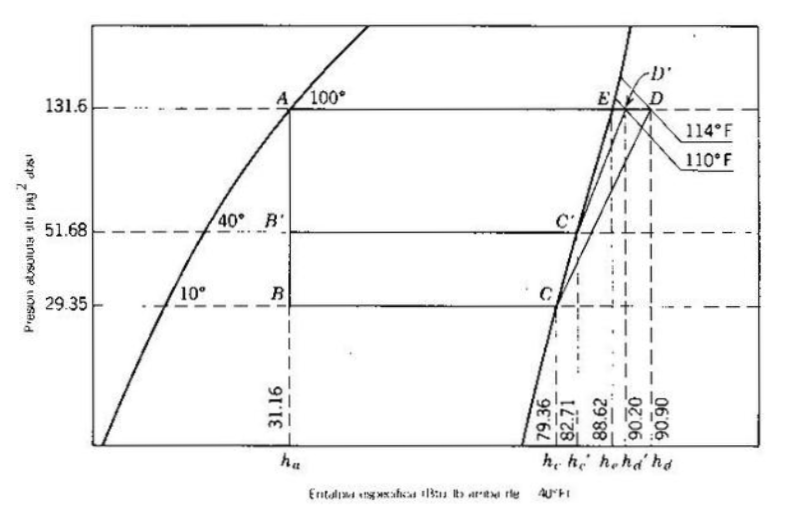
\includegraphics[width=.95\linewidth]{efecto-t-evaporador}
			\caption{Comparación entre dos ciclos saturados simples que trabajan a diferentes temperaturas vaporizantes.}
			\label{fig:efecto-t-evaporador}
		\end{figure}
		
		Uno de los dos ciclos identificados por los puntos A, B, C, D y E, el evaporador está trabajando a una temperatura de $10$ °F y el condensador a una temperatura de $100$ °F, y en los puntos A, B', C', D', y E, se tiene un ciclo similar que tiene la misma temperatura condensante pero que está trabajando a una temperatura vaporizante de $40$ °F.
		
%		Al comparar los dos ciclos se observa que el efecto refrigerante por unidad de masa es mayor para el ciclo que tiene mayor temperatura, esto debido a que se tiene un diferencial menor de temperatura entre la temperatura de baja y de alta.
		Al comparar los dos ciclos se observa que el efecto refrigerante por unidad de masa es mayor para el ciclo que tiene mayor temperatura de vaporización. Este hecho se debe a que el fluido debe ceder menos cantidad de calor para enfriarse a sí mismo a la temperatura del evaporador (proceso expuesto en la  \autoref{sec:ciclo-teorico}). \\
		
		
		\textit{En resumen, a mayor diferencial de temperatura o presión entre el condensador y el evaporador, menor será el efecto refrigerante por unidad de masa.}\\
		
		
		Por otro lado, el trabajo de compresión por unidad de masa necesario para comprimir al vapor desde la presión vaporizante hasta la presión condensante es menor para el ciclo de menor diferencial de temperatura.
		
		De manera similar, cuanto mayor sea el valor de caída de temperatura (o presión), mayor será el volumen específico y por tanto, menor será el desplazamiento volumétrico del compresor (la masa de refrigerante circulado por un compresor será menor)\footnote{En otras palabras, por cada kilogramo de refrigerante en circulación, el compresor deberá comprimir un volumen mayor de vapor.}.
		
		
		Cabe destacar que el aumento en porcentaje del volumen comprimido es mucho mayor que el aumento en porcentaje del caudal másico, lo cual, es probable que esto sea uno de los factores más importantes que influyen en la capacidad y eficiencia de un sistema de refrigeración y por consiguiente sea el más observado. Siguiendo el ejemplo expuesto en el libro (\cite[páginas 137 a 140]{dossat2004refrigeracion}), se observa que el aumento en masa es del $6.5\%$, mientras que el aumento en volumen es de $45\%$.
		
	
		\subsubsection{Efecto de la temperatura de descarga}
		
		En general, si la temperatura vaporizante se mantiene constante, disminuirá la eficiencia del ciclo al aumentarse la temperatura condensante.
		
		
		Para mostrar el efecto de la temperatura condensante sobre la eficiencia del ciclo, en la \autoref{fig:efecto-t-condensador} se muestra un diagrama \emph{ph} de dos ciclos diferentes. El ciclo A, B, C, D y E, es el cual tiene una temperatura condensante de $100$ °F, mientras que el ciclo A', B', C, D' y E', trabaja a $120$ °F.
		
		\begin{figure}[H]
			\centering
			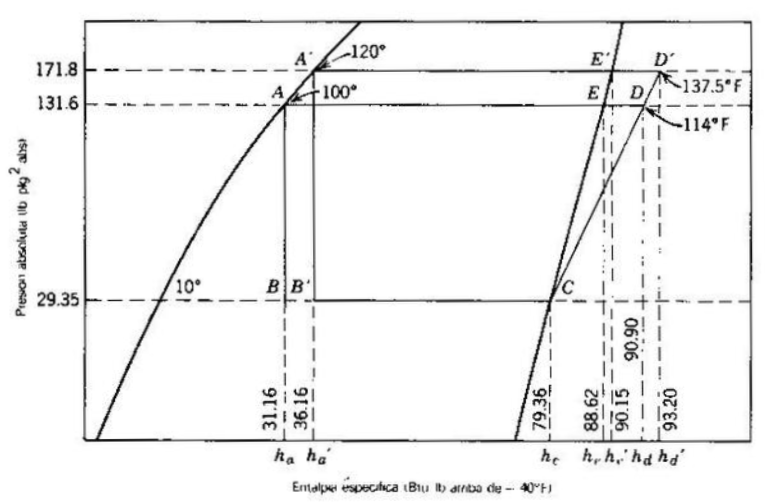
\includegraphics[width=.9\linewidth]{efecto-t-condensador}
			\caption{Comparación entre dos ciclos saturados simples que trabajan a diferentes temperaturas condensantes.}
			\label{fig:efecto-t-condensador}
		\end{figure}
		
		A medida que se aumenta la temperatura condensante, se aumenta también la temperatura que llega a la válvula de expansión y se reduce el valor del efecto refrigerante. En consecuencia, el caudal de masa del refrigerante será mayor.
		
		
		Ya que el caudal de masa es mayor para la temperatura condensante más alta, se deduce que el volumen de vapor comprimido es también mayor. Realizando un análisis, se puede observar que el aumento en porcentaje en el volumen de vapor manejado por el compresor es exactamente igual al porcentaje de aumento del caudal másico. Esto contrasta con lo que sucede cuando es variada la temperatura vaporizante.
		
		% 
		Por otro lado, debido a que la diferencia entre las presiones es grande, el trabajo de compresión por unidad de masa será mayor para el ciclo que tenga la mayor temperatura condensante. Como resultado de esto, la potencia teórica requerida también aumentará.
		
		
	\subsection{Ciclo de refrigeración real}
	
	Capítulo 9 del libro
	
		En los ciclos reales de refrigeración se tienen en cuenta ciertas consideraciones que no se contemplaron en el ciclo teórico, como la caída de presión que experimenta el fluido al paso por tuberías, evaporador, condensador, etc. Además, se considerará el subenfriamiento del líquido y el sobrecalentamiento del vapor en la tubería de succión.
		
		
		Los efectos que fueron despreciables en el ciclo teórico, y por tanto los que se considerarán en el ciclo real de refrigeración se enlistan a continuación:
		\begin{itemize}
			\item Sobrecalentamiento en el vapor de succión
			% 8-3 Sobrecalentamiento sin aprovechamiento del enfriamiento
			% 8-4 Sobrecalentamiento con aprovechamiento del enfriamiento
			% 8-5 Sobrecalentamiento en la tubería de succión (sí o sí es no aprovechado, debe aislarse la tubería): explicación de la generación de escarcha
			% 8-6 Sobrecalentamiento del vapor en el espacio refrigerado. Acá menciona la "tubería secadora"
			\item Subenfriamiento en el líquido
			% 8-7 Subenfriamiento en el líquido. Con subenfriador, o torre de enfriamiento
			% 8-8 Intercambiadores de calor. Se utilizan para subenfriar el líquido antes de la válvula de expansión. Ya que es inevitable el sobrecalentamiento del vapor de la succión en un ciclo real, sea que se uso o no un intercambiador de calor, vale la pena cualquier medio práctico que se emplee para aprovechar el enfriamiento del líquido que se tiene en el sobrecalentamiento del vapor.
			\item Pérdidas de fricción
			% 8-9 Pérdidas debidas a la fricción, en tuberías y en válvulas. Para cualquiera caso, en el lado de descarga del compresor la pérdida resulta en un aumento (inevitable) de presión y en el lado de succión, una disminución. En el resto de elementos siempre es una caída de presión. Ver diagrama
			
			
		\end{itemize}
	
	
	\section{Compresores}

Es el coraz\'on de la instalaci\'on. Su funci\'on, dentro del sistema de refrigeración, consiste en aspirar el fluido refrigerante a baja presi\'on y temperatura tales que se pueda condensar.

Lo escrito en esta secci\'on esta basado en el libro \textit{Manual de refrigeración} de \cite[cap\'itulo 3]{Franco2016Manual}.

Los tipos de compresores m\'as empleados en la refrigeración son:

\begin{itemize}
	\item Alternativos 
	\item De tornillo o helicoidales
	\item Rotativos
	\item Centr\'ifugos
\end{itemize}

\subsection{Alternativos}

Pueden ser de simple efecto o de doble efecto, seg\'un realice la compresi\'on del fluido en un solo lado del pist\'on o en ambos lados. Los m\'as utilizados son los de simple efecto.

\subsubsection{Elementos del compresor}

\textbf{Bloque}

El bloque aglutina y soporta todos los elementos del compresor, tanto como fijos como m\'oviles. La parte superior es la culata y la inferior, por su interior, el c\'arter.

\begin{figure}[H]
	\centering
	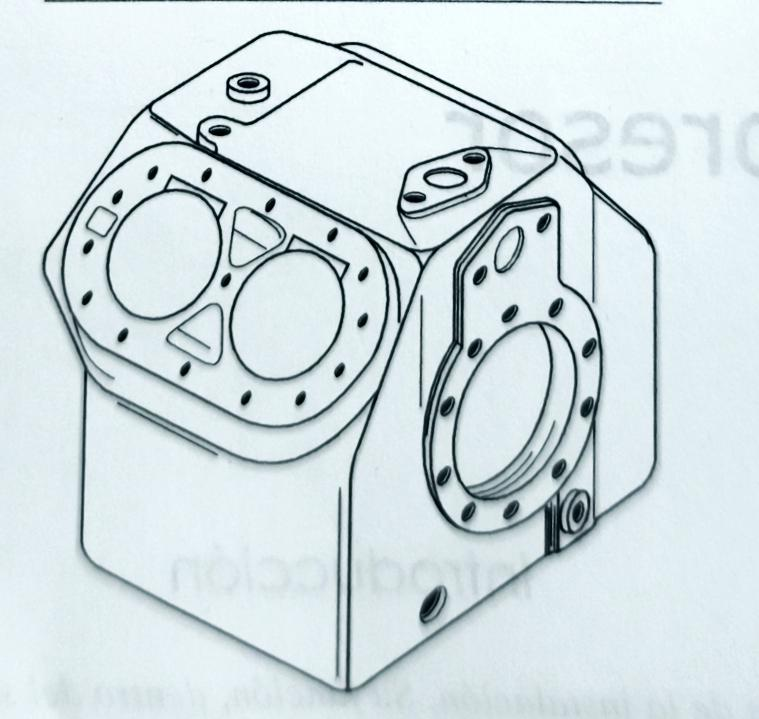
\includegraphics[width=.5\linewidth]{figuras/compresores/bloque}
	\caption{Bloque de un compresor}
	\label{fig:Bloque de un compresor}
\end{figure}

\textbf{C\'arter}

Es el espacio interior comprendido entre el eje cig\"ue\~{n}al y el fondo del bloque, destinado a almacenar el aceite de lubricación.

\textbf{Cilindro}
\begin{wrapfigure}{r}{0.4\linewidth}
	\centering
	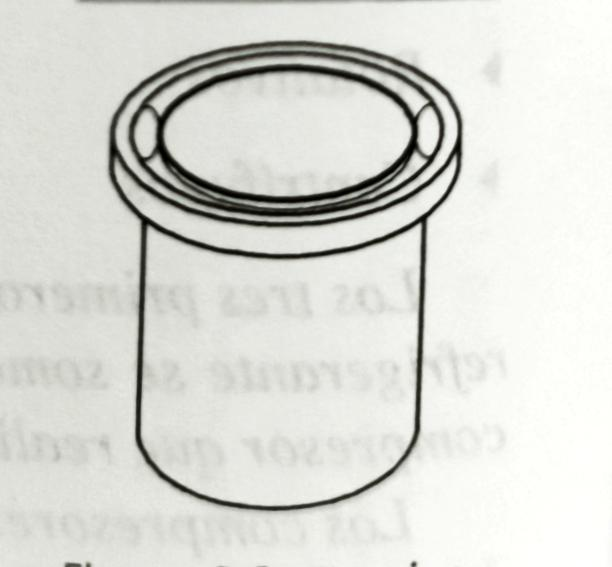
\includegraphics[width=.5\linewidth]{figuras/compresores/cilindro con camisa.jpg}
	\caption{Camisa}
	\label{fig:Camisa}
\end{wrapfigure}
Espacio donde va alojado el pist\'on. En su interior, \'este se desplaza en movimiento rect\'ilineo alternativo. En compresores de mediana y gran potencia (\autoref{fig:Camisa}) lleva camisa, que es una pieza cil\'indrica de acero que lo reviste, y que en casos de desgaste se puede rectificar, o sustituir si procede.

\textbf{Pist\'on o \'embolo}

Elemento que,desplaz\'andose en el interior del cilindro, provoca la aspiraci\'on, compresión y descarga del fluido refrigerante. Lleva alojados los aros o segmentos, que pueden ser:
\begin{itemize}
	\item Aros de engrase: Permiten la lubricación de los cilindros y, en su movimiento, arrastran el aceite al c\'arter.
	\item Aros de compresi\'on: Impiden que el fluido refrigerante escape por los espacios entre el pist\'on y el cilindro, hacia la parte inferior (c\'arter). Esto se aprecia mejor durante la compresi\'on, ya que si hay fugas no se alcanzan las altas presiones necesarias.
\end{itemize}
\textbf{Biela}\\
La biela (\autoref{fig:Conjunto biela-pist\'on y aros}) es el elemento que uno el pist\'on con el eje cig\"ue\~{n}al. Transforma el movimiento circular del eje cig\"ue~{n}al en rectil\'ineo alternativo del pist\'on. Por ello son resistentes y ligeras. La parte superior se llama pie de biela y se une al pist\'on por medio de un bul\'on para evitar el desplazamiento lateral de \'este. Y la parte inferior se llama cabeza de biela y se uno al eje cig\"ue\~{n}al. La biela puede ser de dos tipos, seg\'un se conecte al eje cig\"u\~{n}alo a una exc\'entrica.
\begin{figure}[H]
	\centering
	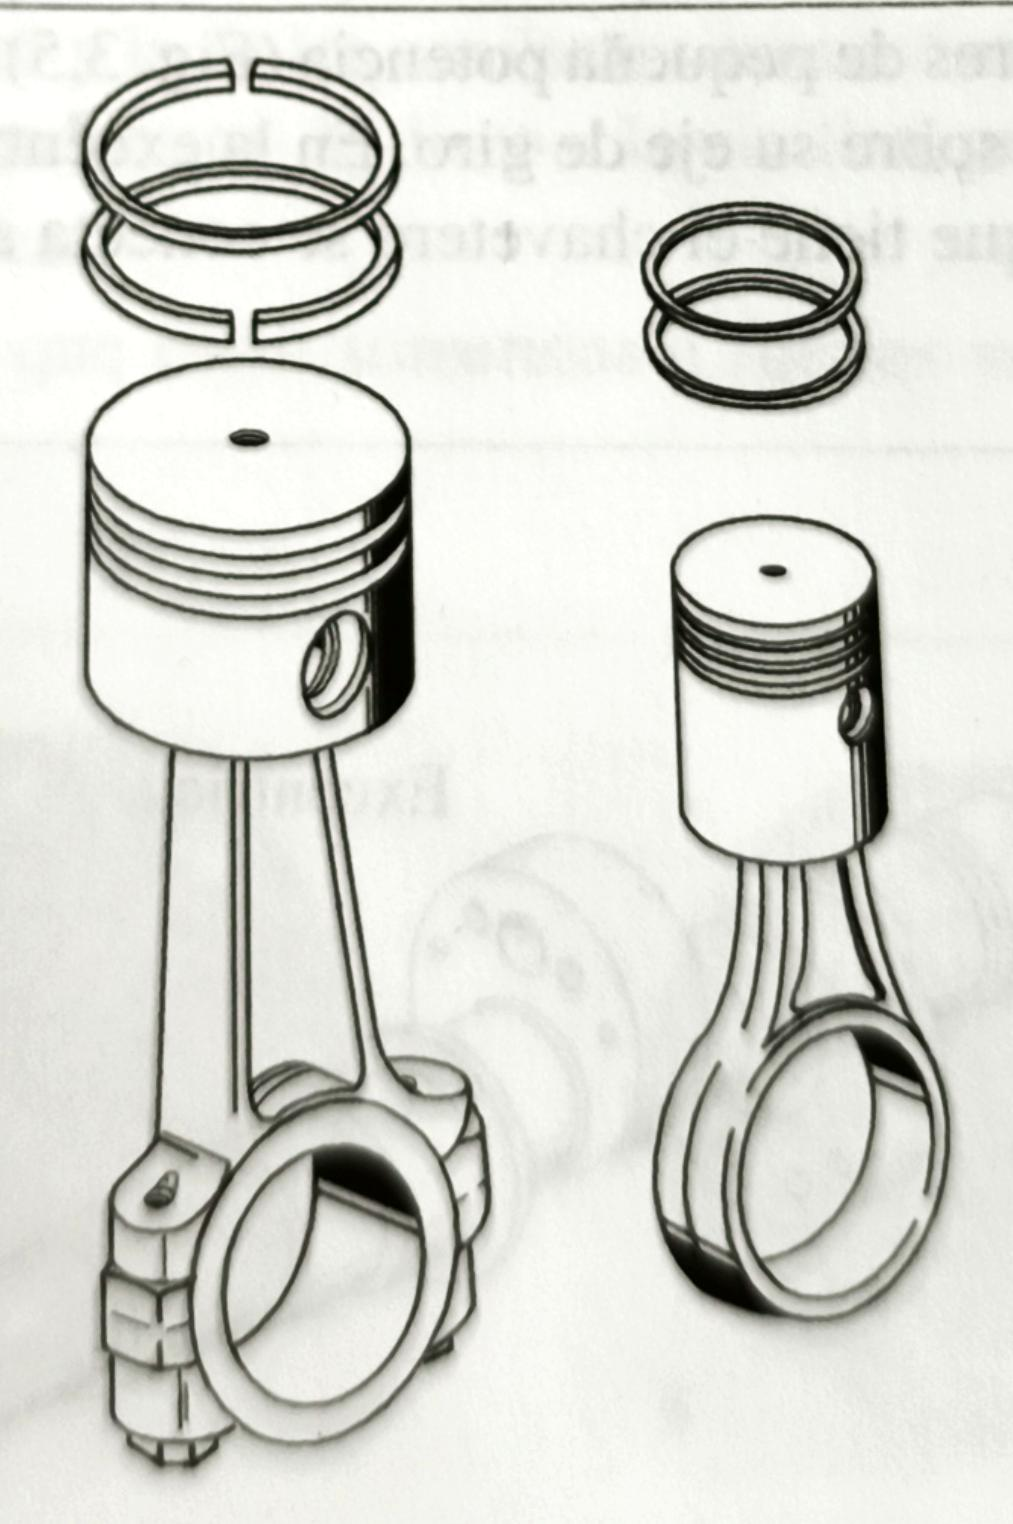
\includegraphics[width=.3\textwidth]{figuras/compresores/piston y biela.jpg}
	\caption{Conjunto biela-pist\'on y aros}
	\label{fig:Conjunto biela-pist\'on y aros}
\end{figure}

\textbf{Eje cig\"ue\~{n}al}\\
La disposici\'on y forma dependen del n\'umero de cilindros (\autoref{fig:Eje cigueñal}). Est\'a formado por un n\'umero determinado de manivelas, que tienen en sus respectivos lados opuestos unos contrapesos de equilibrado. La manivela es la part eque se coencta a la biela.\\
Los extremos del eje, llamados cuellos o mu\~{n}equillas, son los soportes que se apoyan sobe la bancada del compresor. El extremo del eje que tiene el chavetero es el que se conecta al motor el\'ectrico para su accionamiento. El otro extremo acciona la bomba de lubricación.
\begin{figure}[H]
	\centering
	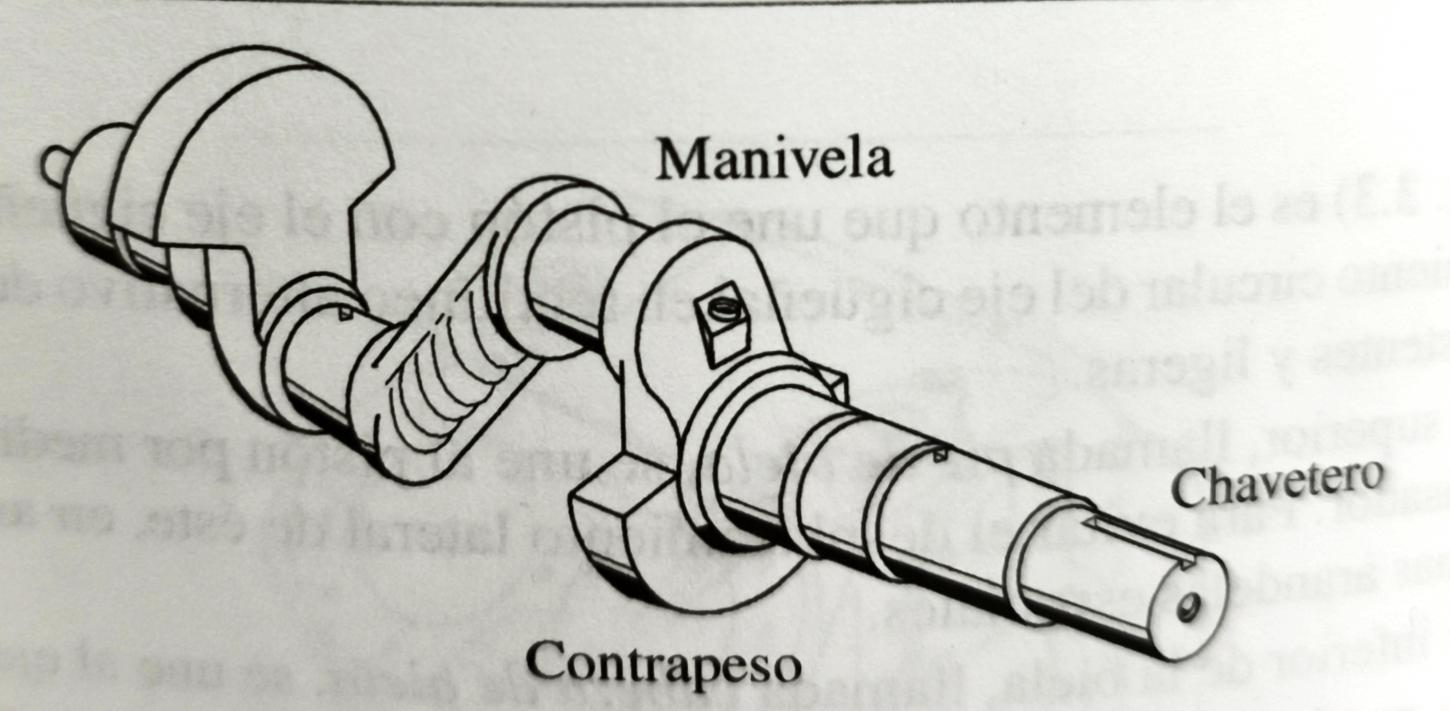
\includegraphics[width=.5\textwidth]{figuras/compresores/eje cigueñal.jpg}
	\caption{Eje cigueñal}
	\label{fig:Eje cigueñal}
\end{figure}
\textbf{Eje de exc\'entrica}\\
Se emplea en compresores de peque\~{n}a potencia (\autoref{fig:Eje de exc\'entrica}). Act\'ua de forma exc\'entrica, de ah\'i el nombre, sobre su eje de giro. En la exc\'entrica se monta la biela. El extremo del eje que tiene el chavetero se conecta al motor el\'ectrico.
\begin{figure}[H]
	\centering
	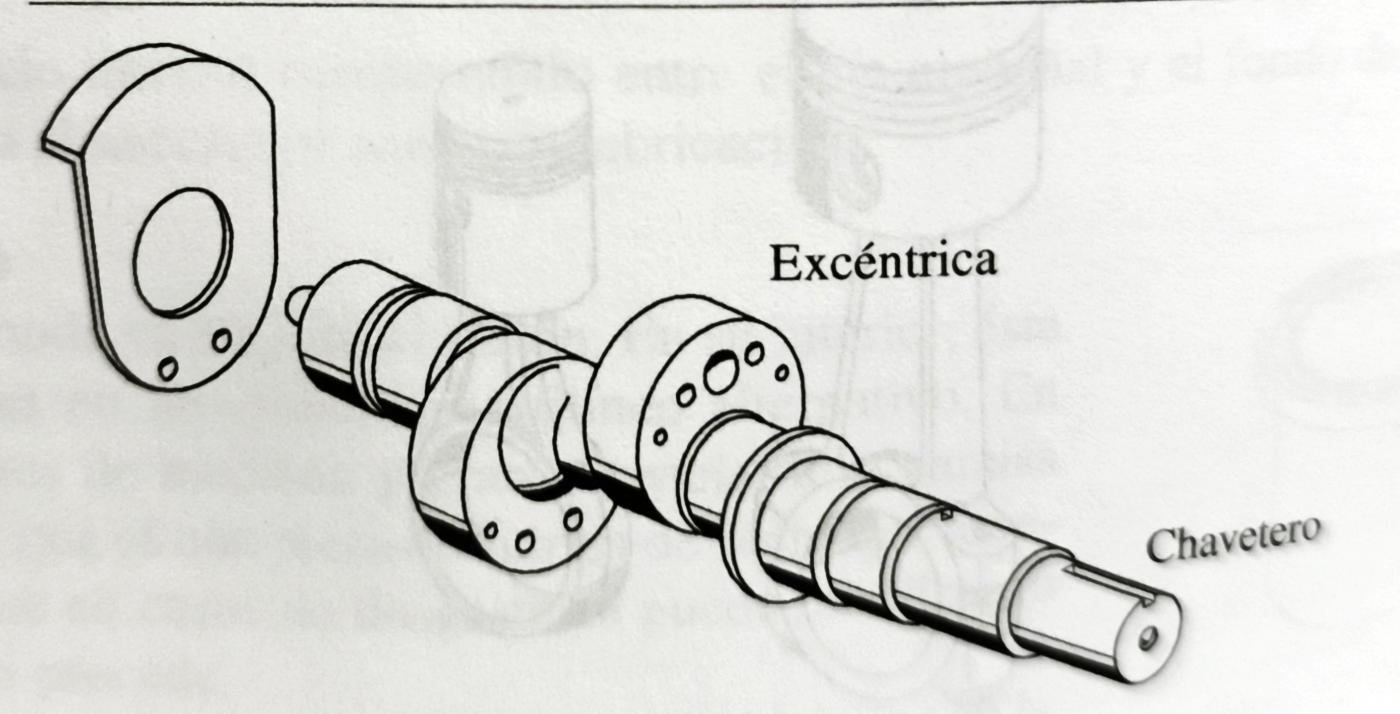
\includegraphics[width=.5\textwidth]{figuras/compresores/eje excentrico.jpg}
	\caption{Eje de exc\'entrica}
	\label{fig:Eje de exc\'entrica}
\end{figure}
\textbf{Culata}\\
Cierra el cilindro por la parte superior. Es la ``tapa'' del cilindro. En ella se alojan las v\'alvulas de aspiración y descarga. Como est\'a sometida a altas temperaturas puede ser refrigerada por aire o por agua (\autoref{fig:Culatas refrigeradas por aire y por agua}).
\begin{figure}[H]
	\centering
	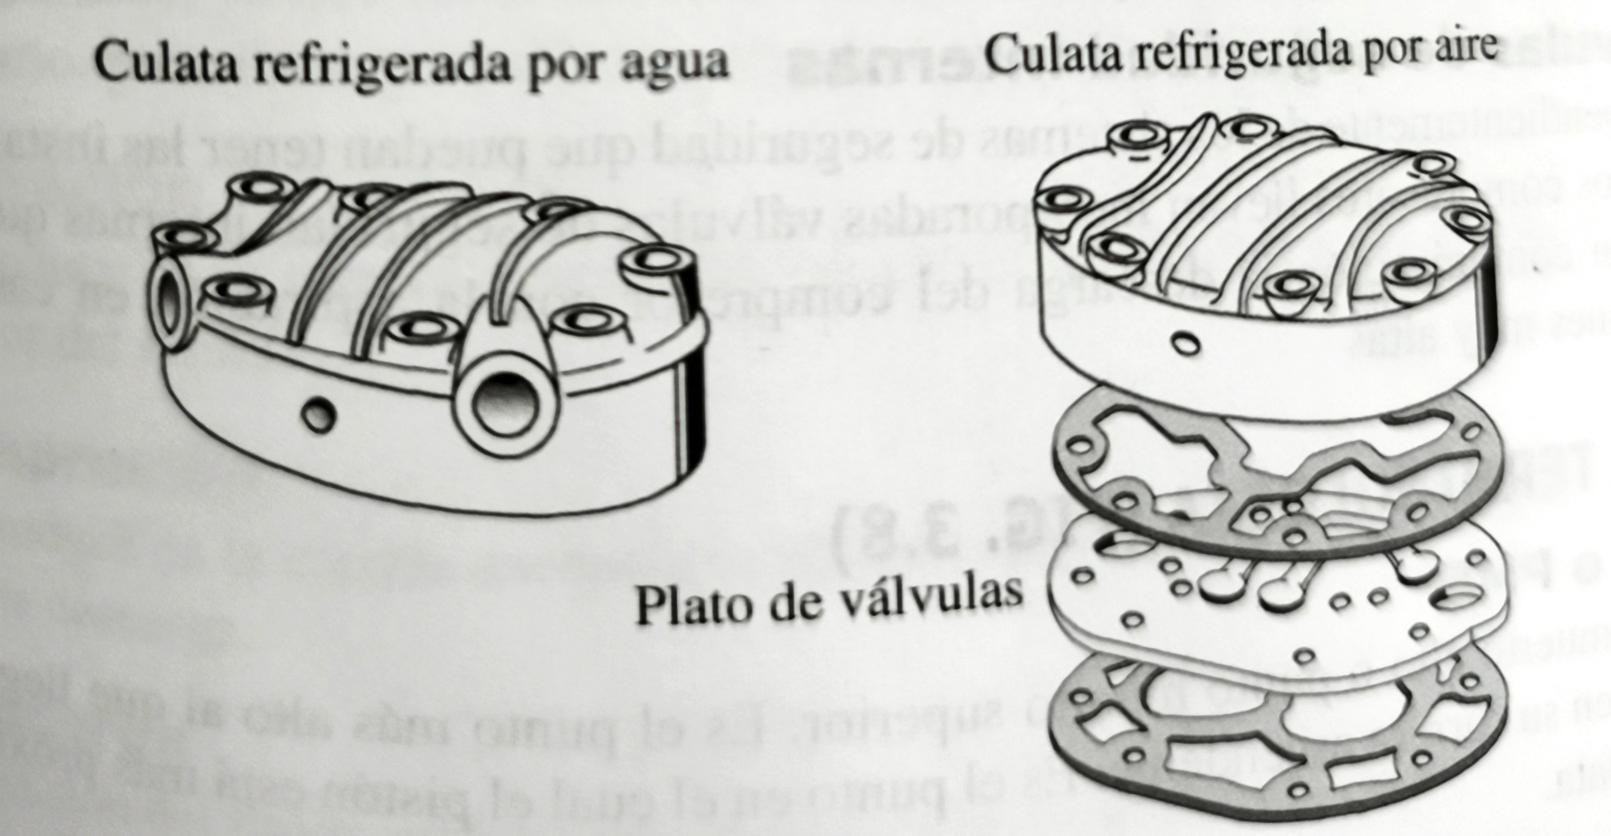
\includegraphics[width=.5\textwidth]{figuras/compresores/culata.jpg}
	\caption{Culatas refrigeradas por aire y por agua}
	\label{fig:Culatas refrigeradas por aire y por agua}
\end{figure}
\textbf{V\'alculas de aspiración y descarga}\\
Se encargan de comunicar el interior del cilindro con los conductos de aspiraci\'on y descarga. Su apertura y cierre se producen por la diferencia de presiones entre la del interior del cilindro y la de los conductos respectivos del fluido. Por lo general son de acero inoxidable, y para grandes potencias, dispotnen de resortes para su accionamiento.\\
\textbf{V\'alvulas de seguridad internas}\\
Independientemente de los sistemas de seguridad que puedan tener las instalaciones, los compresores llevan incorporadas v\'alvulas de seguridad internas que ponen en comunicaci\'on la descargas del compresor con la aspiración en caso de presiones muy altas.

%\subsubsection{Terminología}

%\textbf{PMA o PMS}\\
%Punto muerto alto o punto muerto superio. Es el punto m\'as alto al que llega el pist\'on en su carrera ascendente. Es el punto en el que \'el pist\'on est\'a m\'as cerca de la culata.\\
%\textbf{PMB o PMI}\\
%Punto muerto bajo o punto muerto inferior, es el punto m\'as bajo al que llega el pist\'on en su carrera.\\
%\textbf{Carrera}\\
%Distancia entre el PMS y el PMI. Corresponde a un \'angulo de giro de 180° del cig\"ue\~{n}al.
%
%\begin{figure}[H]
%	\centering
%	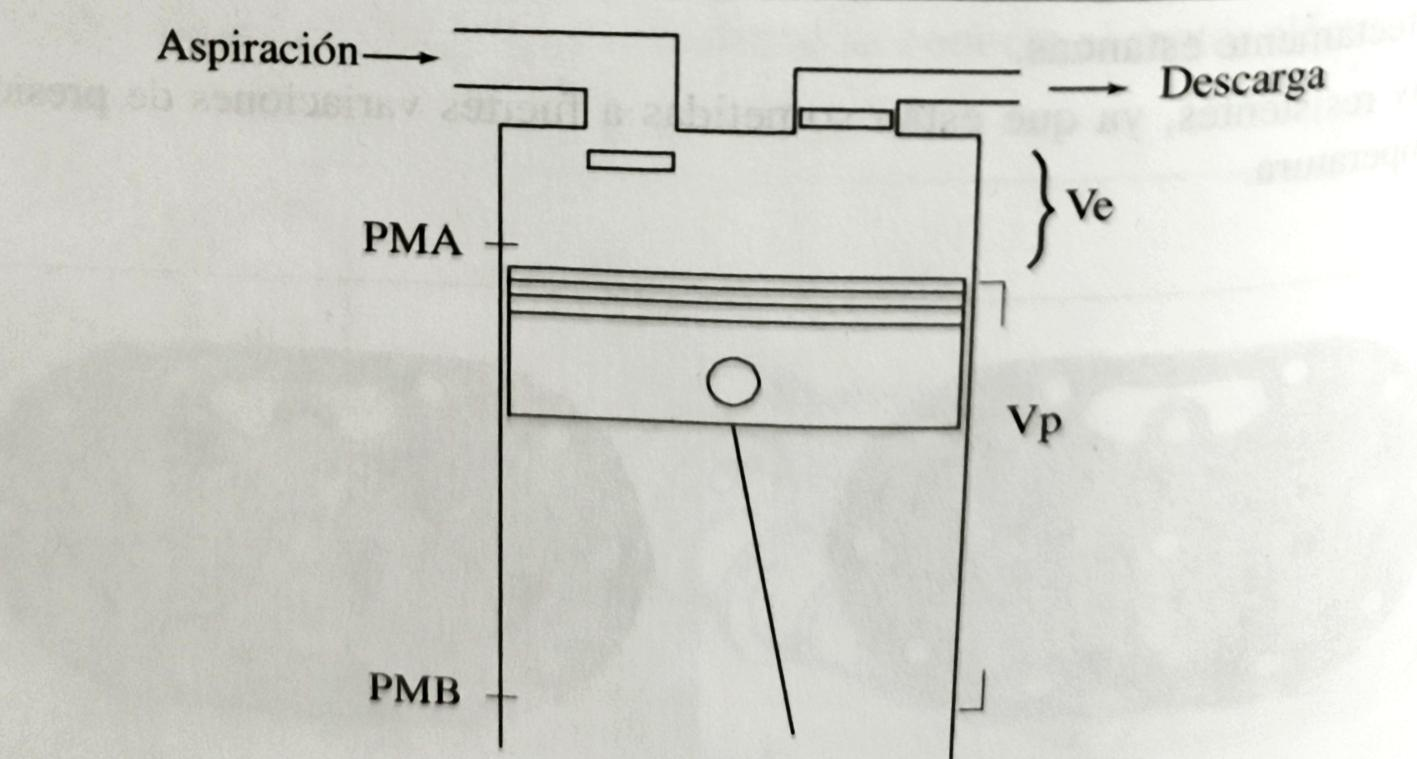
\includegraphics[width=.5\textwidth]{figuras/compresores/terminologia.jpg}
%	\caption{Terminolog\'ia de un cilindro en un compresor}
%	\label{fig:Terminolog\'ia}
%\end{figure}
%
%\textbf{Espacio neutro (Ve)}\\
%Es el comprendido entre el pist\'on cuando se encuentra en el PMS y la culata. Tambi\'en conocido como ``espacio muerto''.Tiene gran importancia en el rendimiento del compresor y est\'a determinado para evitar que el pist\'on, en su carrera ascendente, llegue a chocar con la culata, incluyendo las dilataciones que sufren los materiales, ya que est\'an sometidos a altas temperaturas. Debe ser el m\'inimo necesario, pues tiene gran repercusi\'on en el rendimiento volum\'etrico.\\
%\textbf{Aspiraci\'on}\\
%Se produce en la carrera descendente del pist\'on. Es la admisi\'on del fluido en el interior del cilindro.\\
%\textbf{Compresi\'on}\\
%Se produce en la carrera ascendente del pist\'on e inmediatamente despu\'es se realiza la descarga.\\
%\textbf{Descarga}\\
%Impulsi\'on del fluido refrigerante al conducto de descarga.\\
%\textbf{Volumen desplazado por el pist\'on (Vd)}\\
%El comprendido entre el PMS y PMI que desplaza el pist\'on en la carrera.\\
%\textbf{Volumen total del cilindro (Vt)}\\
%El comprendido entre el pist\'on cuando se encuentra en el PMI y la culata.
%\begin{equation*}
%	Vt = Ve + Vd
%\end{equation*}
%\textbf{Potencia indicada}\\
%Es la potencia que se genera en el interior del cilindro.\\
%\textbf{Potencia efectiva}\\
%Es la potencia que se debe suministrar con el motor el\'ectrico para que el compresor trabaje en las condiciones previstas. Es decir, es la potencia medida en el eje del compresor. Pero a partir de este punto se produce una disminuci\'on de la potencia ya que una parte de la misma se pierde en vencer los rozamientos de cojinetes, bielas, etc. Por ello, la potencia efectiva siempre ser\'a superior a la potencia indicada.
%\begin{equation*}
%	Pe > Pi
%\end{equation*}
%La potencia efectiva es la potencia de accionamiento.\\
%\textbf{Rendimiento mec\'anico}\\
%Es el valor que contempla las p\'erdidas de origen mec\'anico anteriormente mencionadas. Por lo tanto, es la relaci\'on entre ambas potencias:
%\begin{equation*}
%	\eta m = \frac{Pi}{Pe}
%\end{equation*}
\subsubsection{Funcionamiento}
Para facilitar su comprensi\'on vamos a ver como se producen los movimientos de apertura y cierre de las v\'alvulas de aspiraci\'on y descarga, con relaci\'on al movimiento del pist\'on.
\begin{enumerate}[a.]
	\item Carrera descendente:\\ Cuando el pistçón inicia la carrera descendente, hacia el PMI, crea en el interior del cilindro una depresi\'on que implica, que en su interior la presi\'on sea inferior a la existente en la parte superior de la v\'alvula, es decir en el conducto de aspiraci\'on, con lo que la v\'alvula de aspiraci\'on se abre (``baja'') y el fluido refrigerante entra en el cilindro.\\ El fluido entrar\'a en el cilindro hasta que se igualen las dos presiones, y en teor\'ia deber\'ia ser en cantidad igual a la correspondiente al volumen del cilindro, pero hay factores que impiden que entre esa cantidad.\\ La v\'alvula de descarga permanece cerrada, por la alta presi\'on existente en el conducto de descarga mientras el pist\'on se va acercando al PMI y la v\'alvula de aspiraci\'on contin\'ua abierta.\\ As\'i, cuando el pist\'on llega al PMI, la v\'alvula de aspiraci\'on est\'a abierta y la de descarga cerrada. El cig\"ue\~{n}al ha girado 180°.
	\item Carrera ascendente:\\ Cuando el pist\'on rebasa el PMI se inicia la carrera ascendente, y la v\'alvula de aspiraci\'on se cierra, porque la presi\'on en el interior del cilindro es superior a la existente en el conductor de aspiraci\'on. Con las dos v\'alvulas cerradas se inicia la compresi\'on del fluido (\autoref{fig:Carrera ascendente}A), y se produce:
	\begin{itemize}
		\item Una disminici\'on de volumen.
		\item Un aumento de la presi\'on y la temperatura, hasta que la primera alcanza un valor tal que hace que se abra (levante) la v\'alvula de descarga.
	\end{itemize}
	En la \autoref{fig:Carrera ascendente} se puede apreciar que poco antes de que el pist\'on llegue al PMS la v\'alvula de descarga abre (``hacia afuera''), porque la presi\'on en el interior del cilindro, en la carrera escendente, es superior a la del conducto de descarga y ``levanta'' la v\'alvula. El fluido es impulsado hacia el condensador.\\
	El cig\"ue\~{n}al ha girado 180°, con lo que las dos carreras consecutivas gir\'o 360°, es decir una vuelta.\\ Una vez rebasado el PMS, y con la v\'alvula de descarga cerrada, se reinicia el ciclo.
\end{enumerate}
\begin{figure}[H]
	\centering
	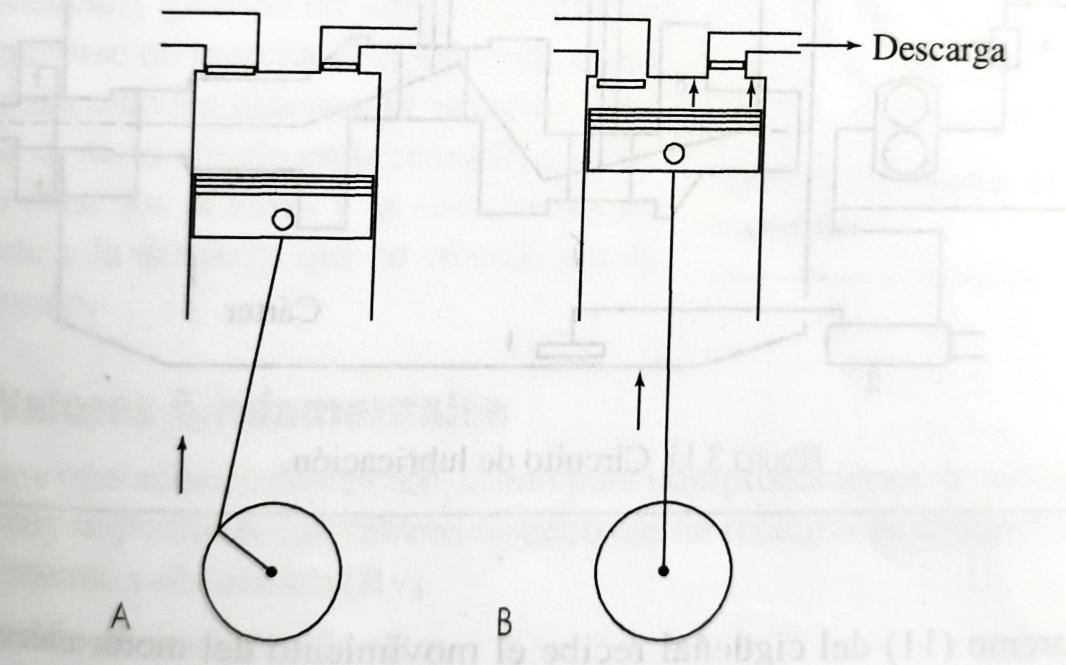
\includegraphics[width=.5\linewidth]{figuras/compresores/aspiracion y descarga.jpg}
	\caption{A = Compresi\'on. B = Descarga}
	\label{fig:Carrera ascendente}
\end{figure}
\subsubsection{Lubricación}
Es uno de los asprectos m\'as importantes del compresor y por lo tanto de la instalaci\'on. El tipo de lubricaci\'on empleada es forzada, mediante una bomba de engranajes que es accionada por el mismo motor el\'ectrico que acciona el compresor.\\ Anteriormente hemos comentado que a trav\'es de los aros de engrase, el aceite sale impulsado hacia las camisas. Pero tambi\'en se lubrican otras partes en movimiento como el cigueñal, cojinetes de bancada, cojinetes de biela y prensas principales.

Es importante saber que el circuito de aceite que conecta la bomba de engranajes con los dispositivos a lubricar cuenta con filtros y un enfriador de aceite, ya que este, adem\'as de lubricar, refrigera los elementos. El compresor tendr\'a enfriador de aceite dependiendo de su potencia, tipo y caracter\'isticas de funcionamiento.
\subsubsection{Valores fundamentales}
Tanto para operaciones de c\'alculo, como para comprobaciones de funcionamiento, son muy importantes los valores respectivos de relaci\'on de compresi\'on (Rc) y de rendimiento volum\'etrico (Rv).
\begin{enumerate}[1.]
	\item \textbf{Relaci\'on de compresi\'on (Rc)}
	\begin{equation*}
		Rc = \dfrac{\text{Presi\'on de descarga absoluta}}{\text{Presi\'on de aspiraci\'on absoluta}}
	\end{equation*}
	$\text{Presi\'on absoluta = Presi\'on manom\'etrica + Presi\'on atmosf\'erica}$
	\item \textbf{Rendimiento volum\'etrico (Rv)}\\ Se puede expresar de varias maneras, pero una de ellas a efectos pr\'acticos es:
	\begin{equation*}
		Rv = {\frac{\text{Volumen de vapor que realmente aspira}}{\text{Volumen te\'orico que tendr\'ia que aspirar}}X 100}
	\end{equation*}
	Cuanto mayor sea la relaci\'on de compresi\'on, menor ser\'a el rendimiento volum\'etrico y viceversa.

	Su valor depende de factores rales como el espacio neutro y la densidad del fluido en el interior del cilindro.
	\item \textbf{Volumen desplazado}\\ El volumen de fluido que en teor\'ia tiene que aspirar es el volumen desplazado por el pist\'on en su carrera. Como sabemos, el volumen de un cilindro es el producto del \'area por la altura:
	\begin{gather*}
		V = S \times h\\ 
		S = \pi\cdot r^2 = \pi\cdot(\frac{D}{2})^2 = \pi\cdot\frac{D^2}{4}
	\end{gather*}
	y la altura (h) es la distancia entre PMI y el PMS, o sea es la carrera:
	\begin{equation*}
		V = \frac{\pi D^2}{4}C
	\end{equation*}
	que es el volumen que desplaza el pist\'on en una revoluci\'on. Si gira el cig\"ue\~{n}al a n revoluciones por minuto y tiene N cilindros, el volumen desplazado ser\'a:
	\begin{equation*}
		Vd = \frac{\pi\cdot D^2\cdot C\cdot n\cdot N\cdot 60\cdot 10^-3}{4}(\frac{m^3}{h})
	\end{equation*}
\end{enumerate}
\subsection{Compresores herméticos}
Su \'ambito de aplicaci\'on comprende los sitemas de refrigeraci\'on y aire acondicionado.\\El motor el\'ectrico va acoplado directamente al compresor, y ambos dentro de la misma envolvente (carcasa) de acero formando una unidad. Al ser herm\'eticos (cerrados) no podemos acceder a ellos, como por ejemplo, para realizar operaciones de mantenimiento. Pueden ser alternativos, rotativos o de tornillo.\\ En su configuraci\'on (\autoref{fig:Compresor herm\'etico}), lleva tres tubos soldados a la carcasa. Dos son del mismo di\'ametro y el tercero menor. El de menor di\'ametro se conectar\'a a la descarga y la aspiraci\'on a cualquiera de los otros dos. Por lo general, se hace al tubo que est\'a al lado contrario de la placa de conexionado el\'ectrico, para evitr que las condensaciones que se puedan producir en el exterior del mismo, lleguen a introducirse a la placa.\\ De esta manera el otro tubo, que no se conecta la circuito, se puede utilizar para que, despu\'es de instalar una conexi\'on ob\'us o una v\'alvula de intervenci\'on, se aproveche para realizar operaciones tales como:
\begin{itemize}
	\item Meter carga de refrigerante
	\item Comprobar la presi\'on de aspiraci\'on
	\item Comprobar la temperatura de evaporaci\'on
	\item Meter aceite
\end{itemize}
\begin{figure}[H]
	\centering
	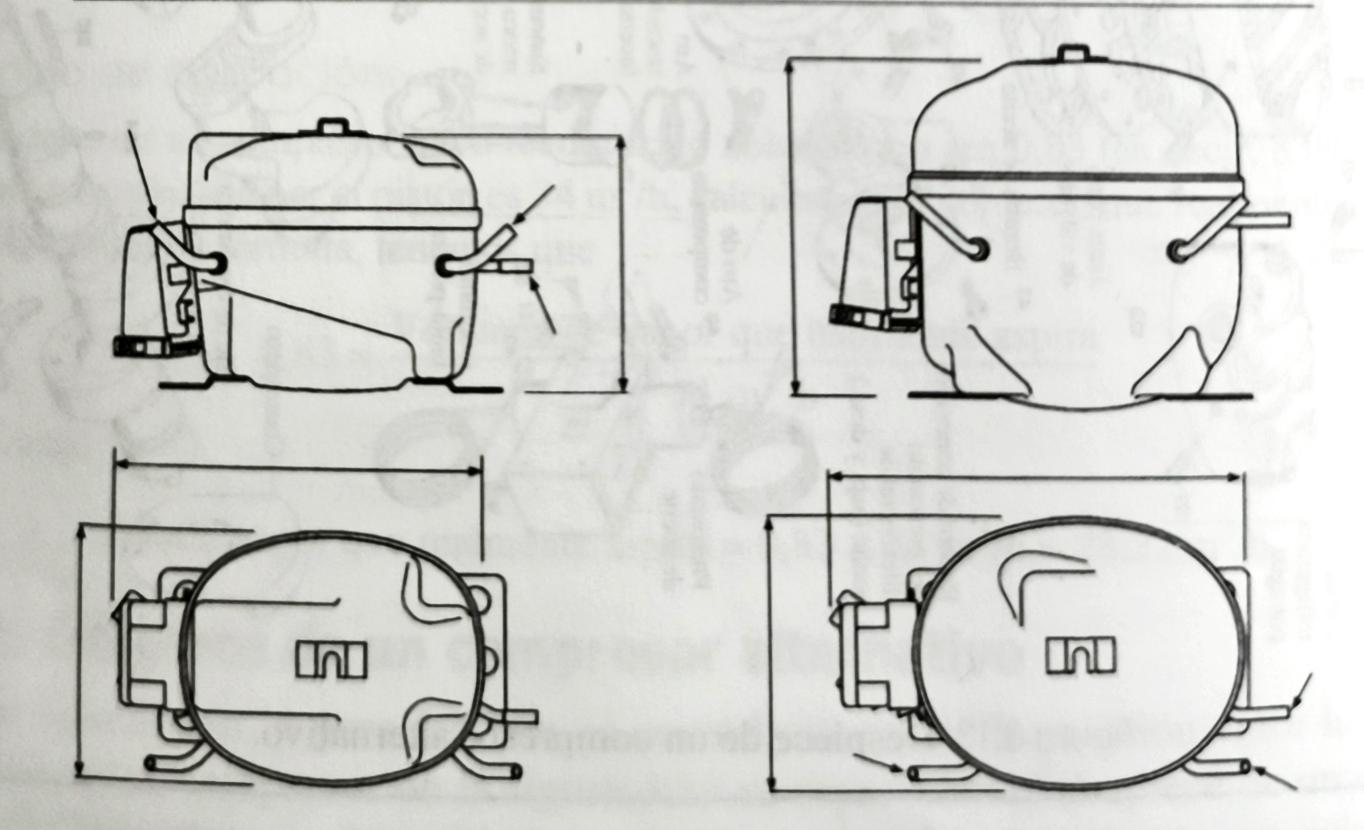
\includegraphics[width=.8\linewidth]{figuras/compresores/compresor herméticos.jpg}
	\caption{Compresor herm\'etico}
	\label{fig:Compresor herm\'etico}
\end{figure}
\subsubsection{Algunas caracter\'isticas}
\begin{enumerate}[1.]
	\item Son silenciosos porque cuentan con resortes interiores y c\'amaras silenciadoras que amortiguan el golpeteo de las v\'alvulas. Carecen de transmisiones exteriores como por ejemplo correas.
	\item Est\'an refrigeradores por el fluido de aspiraci\'on por lo que, la falta de fluido afectar\'ia a la refrigeraci\'on del compresor. Hay que evitar la humedad en el circuito y la entrada de l\'iquido al compresor porque estar\'ian en contacto con la parte el\'ectrica.
	\item Trabajar a temperaturas inferiores a las normales, implicar\'ia el aumento del volumen espec\'ifico, que afectar\'ia, entre otras cosas a la refrigeraci\'on.
\end{enumerate}
\subsection{Compresores semiherméticos}
Estos compresores en su funcionamiento tienen las mismas ventajas e inconvenientes que los herm\'eticos pero a diferencia que son m\'as accesibles para realizar mantenimiento. Por ejemplo, en compresores semiherm\'eticos alternativos se pueden desmontar para realizar operaciones de mantenimiento tales como cambiar pistones o aros.\\ Pueden ser enfriados externamente por aire o por agua.
\subsubsection{\'Acidos}
Es importante comentar que en los compresores, ya sean herm\'eticos o semiherm\'eticos, una de las aver\'ias m\'as importantes es la contaminaci\'on del circuito por \'acidos, puesto que se refrigeran por los vapores de aspiraci\'on. La presencia de \'acidos se produce por altas temperaturas en la zona que se encuentra entre el estator y rotor, esto genera que el fluido refrigerante reaccione y ataque los devanados del estator.\\ Las causas pueden ser varias pero se podr\'ia englobar en mantenimiento inadecuado, sobre carga del motor y elevadas temperaturas de trabajo.\\ Si se cambia un compresor por otro en un sistema contaminado por \'acidos y antes no se eliminan \'estos, atacar\'an a los aislamientos de los bobinados, con lo cual la duraci\'on del nuevo compresor ser\'a muy corta.
\subsection{Compresores abiertos}
Se llaman abiertos porque el motor el\'ectrico y el compresor est\'an separados. Por lo tanto, el fluido refrigerante ya no est\'a en contacto con la parte el\'ectrica, como ocurre en los compresores herm\'eticos y semiherm\'eticos. Como est\'an separados la conexi\'on entre ambos necesita de un sistema de estanqueidad o sello en ese punto para evitar las fugas del fluido refrigerante al exterior. El acoplamiento motor-compresor se puede realizar mediante correas, se puede adaptar la velocidad con sus di\'ametros (seg\'un necesidad de carga) o mediante dos platos met\'alicos unidos el\'asticamente.
\subsubsection{Caracter\'isticas de funcionamiento}
En estos compresores abiertos se considera buena relaci\'on de compresi\'on (Rc) si no excede de 10:1, ya que cuanto menor sea, mayor ser\'a el rendimiento volum\'etrico (Rv) y, por lo tanto, mayor ser\'a la potencia frogir\'ifica.\\ Si el compresor tuviera que trabajar con una Rc elevada, como sucede, por ejemplo, cuando se trata de instalaciones que necesiten temperaturas muy bajas para enfriar y las de condensaci\'on sean normales, entonces no se podr\'ia utilizar uno de simple etapa, porque entre otras cosas, las altas temperaturas afectar\'ian:
\begin{itemize}
	\item A los materiales (dilataciones)
	\item A la lubricaci\'on, perjudicar\'ia la viscosidad del aceite
	\item A las temperaturas de descarga, porque ser\'ian muy altas
	\item Y a los rendientos, que disminuir\'ian
\end{itemize}
Para solucionar estos inconvenientes tendr\'iamos que recurrir a los compresores de doble etapa (sistema compound), que tambi\'en se hace extensivo a los semiherm\'eticos.
\subsubsection{Compresores de doble etapa}
Los compresores de doble etapa reparten la elevada relaci\'on de presiones y disminuyen el alto recalentamiento. Cada secci\'on del compresor trabaja a menor presi\'on y tambi\'en menor temperatura de descarga, lo que implica un mejor aprovechamiento volum\'etrico. Para ello emplean un sistema de enfriamiento en la etapa intermedia, cuando es asi se los llama sistema por \textbf{inyecci\'on parcial}. Pero cuando se enfria el fluido en la etapa intermedia y, a su vez, antes de que \'este entre en el evaporador se lo llama sistema de \textbf{inyecci\'on total}.
\begin{itemize}
	\item \textbf{Inyecci\'on parcial:}\\ Se mezclan el fluido expansionado por la v\'alvula y los gases de descarga de los cilindros de baja en la tuber\'ia de presi\'on intermedia. De esta manera, se logra bajar la temperatura de descarga de los cilindros de alta.
	\item \textbf{Inyecci\'on total}\\ Se realiza un enfriamiento de los gases de descarga de los cilindros de baja y, a su vez, tambi\'en se hacen pasar el fluido expansionado por un intercambiador de calor para enfriar el refrigerante antes de entrar al evaporador e incrementar el efecto frigorífico.
\end{itemize} 
\subsection{Compresores rotativos}
Se caracterizan por comprimir el fluido refrigerante mediante el movimiento circular continuo de un rotor, que puede ser de exc\'entrica o de paletas.
\subsubsection{De exc\'entrica}
\begin{wrapfigure}{r}{0.45\linewidth}
	\centering
	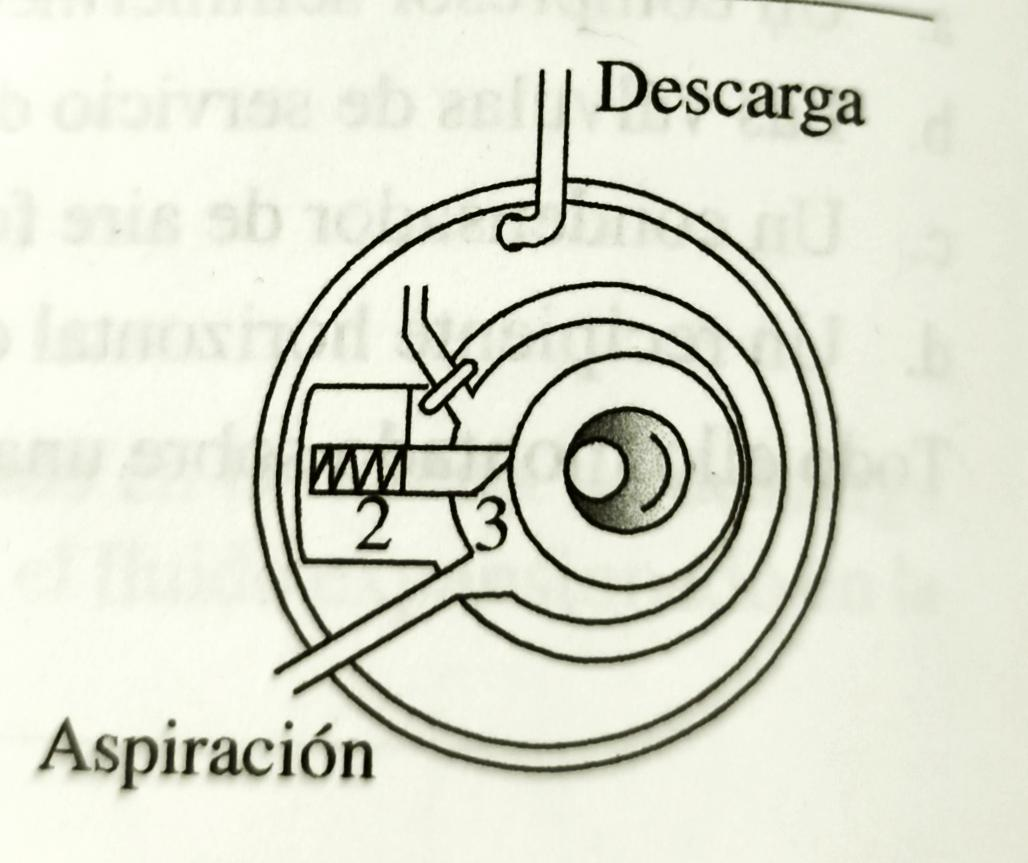
\includegraphics[width=.7\linewidth]{figuras/compresores/rotor de excentrica.jpg}
	\caption{Rotor de exc\'entrica}
	\label{fig:Rotor de exc\'entrica}
\end{wrapfigure}
Consta (\autoref{fig:Rotor de exc\'entrica}) de un rotor exc\'entrico respecto al cilindro donde se aloja y que en su movimiento llega a establecer contacto con \'el.\\Este rotor, por acci\'on del resorte (2) est\'a permanentemente en contacto con una paleta (3).\\Esta paleta, tal como se aprecia en la figura, establece la separaci\'on entre las c\'amaras de aspiraci\'on y de descarga. En su funcionamiento, la aspiraci\'on se realiza de manera continua, y al disminuir el espacio comprendido entre el rotor y el cilindro, se efect\'ua la comprensi\'on del fluido refrigerante y posterior descarga.

\subsubsection{De paletas}

B\'asicamente (\autoref{fig:Rotor de paletas}) consta de un rotor montado en el interior de un cilindro y cuyos centros ent\'an ligeramente desplazados. Este rotor aloja unas paletas que est\'an comprimidas contra la pared del cilindro por medio de unos resortes. Al pasar cada paleta por el orificio de la aspiraci\'on, se crea una depresi\'on que provoca la entrada del fluido en el espacio comprendido entre esa paleta y la anterior. Posteriormete y dado que el espacio entre el rotor y el cilindro disminuye, tambi\'en lo hace el volumen del fluido (compresi\'on) hasta que alcanza el orificio de descarga.\\ Existen compresores cuyos rotores no llevan resortes y las paletas se mantienen comprimidas por la acci\'on de su propio peso y de la fuerza centr\'ifuga.

\begin{figure}[H]
	\centering
	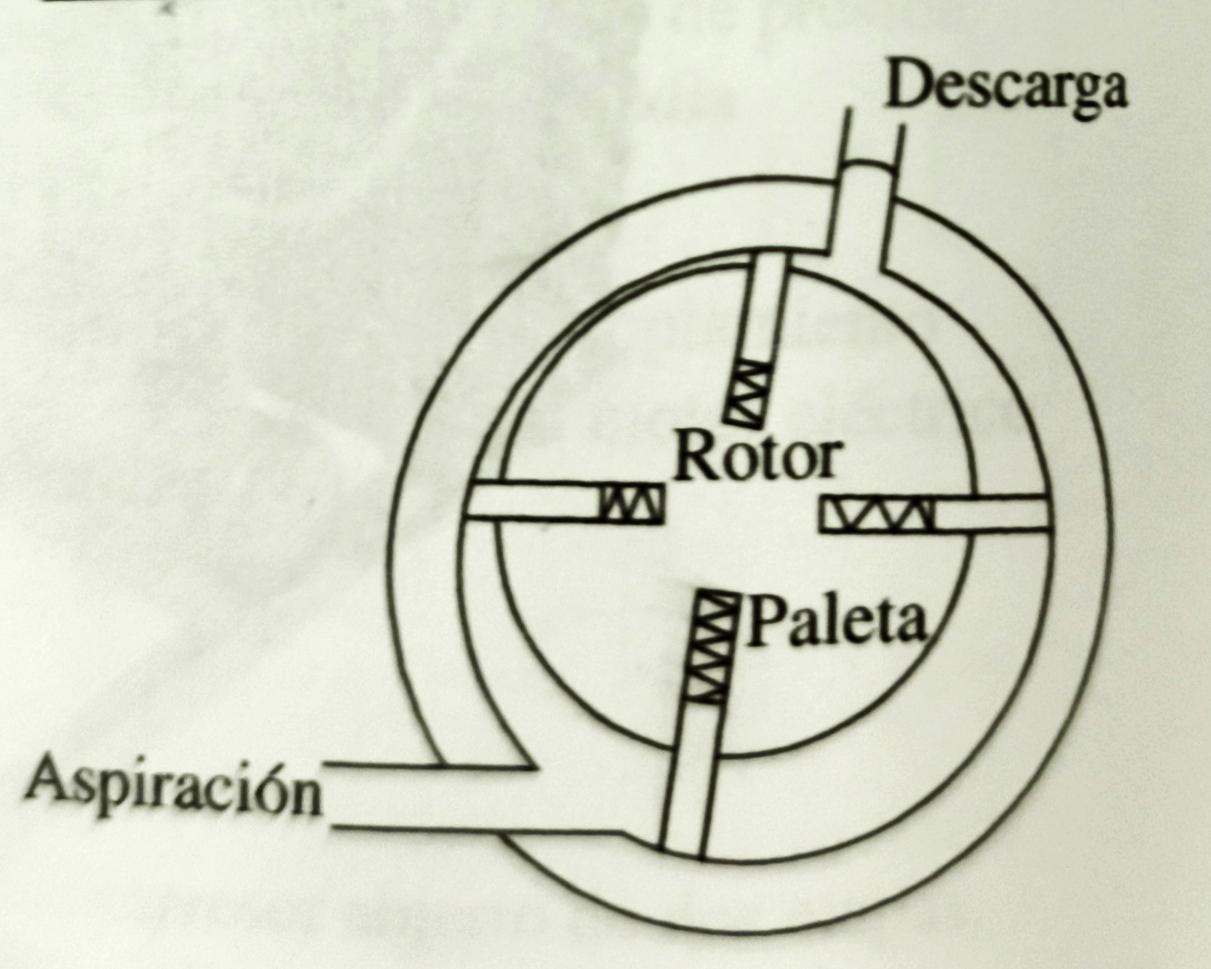
\includegraphics[width=.4\linewidth]{figuras/compresores/rotor de paletas.jpg}
	\caption{Rotor de paletas}
	\label{fig:Rotor de paletas}
\end{figure}

\subsection{Compresores helicoidales}

Los compresores helicoidales o de tornillo son distintos a los anteriormente vistos. La compresi\'on del fluido es continua. Constan de dos rotores llamados primario y secundario que, montados en ambos extremos sobre cojinetes, aseguran su exacta posici\'on en el interior del compresor. El \textbf{rotor primario}, de cuatro l\'obulos o helicoides, es accionado directamente por el motor el\'ectrico y gira a la misma velocidad que \'este.\\ Mediante un sistema de rodamientos, el rotor primario transmite el movimiento al \textbf{rotor secundario}, que tiene seis l\'obulos o helicoides y es del mismo di\'ametro, pero gira a menor velocidad y en sentido contrario.\\ Entre los dos rotores existe una separaci\'on muy pequeña, es decir, no est\'an en contacto entre s\'i.\\Al girar ambos rotores dentro de la cavidad del compresor y debido a esa pequeña separaci\'on, se producen las aberturas de espacios en la zona de aspiraci\'on que con el giro van disminuyendo, con lo que se translada y comprime el fluido hacia el otro extremo de los rotores, donde se produce la descarga del fluido refrigerante.\\ Los hay de tipo herm\'etico, semiherm\'etico y abiertos.
\subsubsection{Importancia del aceite}
Estos compresores helicoidales llevan unos grandes separadores de aceite. Este es inyectado a lo largo de los tornillos para su lubricaci\'on y sellado al mismo tiempo, lo que facilita la compresi\'on del fluido.\\ La \autoref{fig:Circuito de aceite en instalaciones con compresores a tornillo} representa una aplicaci\'on muy utilizada de estos compresores.\\Como consecuencia de la alta temperatura que alcanza el aceite, a la salida del separador y antes de volver al compresor, suele pasar por un enfriador, que seg\'un las caracter\'isticas de la instalaci\'on, puede utilizar aire, agua o el mismo refrigerante para el enfriamiento del aceite.\\ Los factores que determinan si es necesario el enfriamiento del aceite son las condiciones de trabajo:

\begin{itemize}
	\item Temperatura de condensaci\'on
	\item Temperatura de evaporaci\'on
	\item Temperatura de descarga
\end{itemize}

\begin{figure}[H]
	\centering
	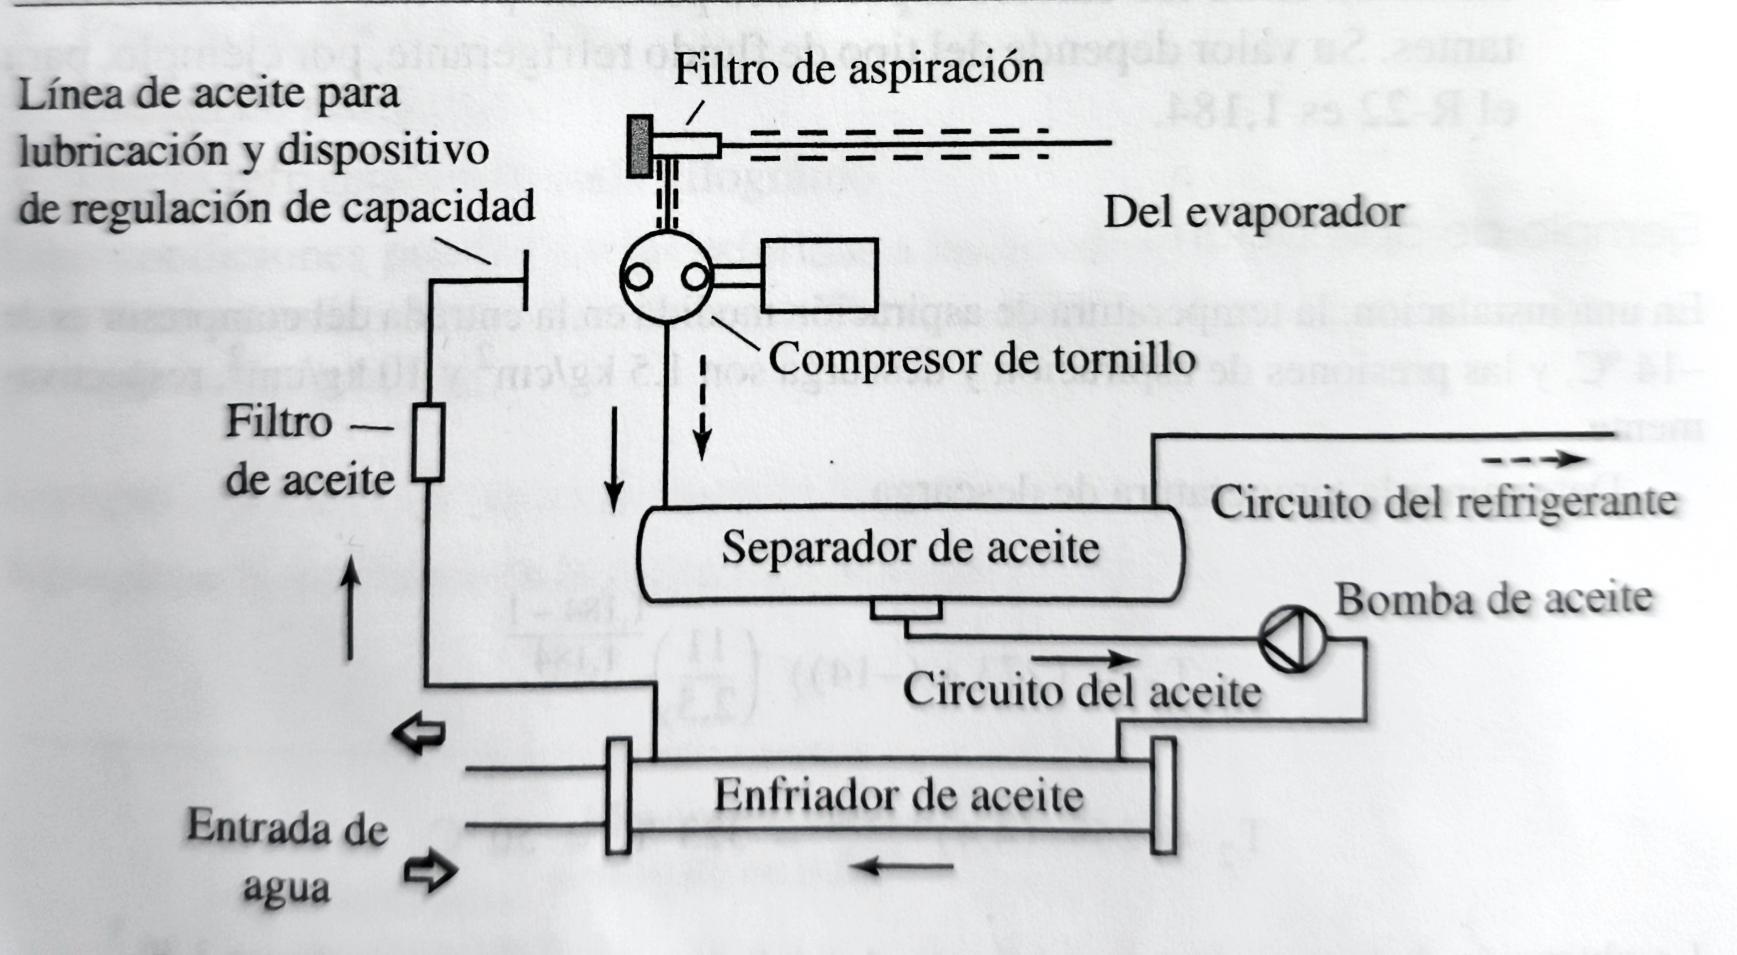
\includegraphics[width=\textwidth]{figuras/compresores/circuito de aceite (2).jpg}
	\caption{Circuito de aceite en instalaciones con compresor a tornillo}
	\label{fig:Circuito de aceite en instalaciones con compresores a tornillo}
\end{figure}

\subsection{Regulación de la potencia}

Si la carga de los evaporadoes siempre fuese la misma, se intalar\'ia el compresor a esa determinada carga t\'ermica. Pero como en la mayor\'ia de los casos la carga var\'ia (ejemplo m\'as notorio lo tenemos en las instalaciones de aire acondicionado), se debe encontrar un punto de equilibrio entre la carga producida por el compresor y la carga necesaria en el evaporador.\\Para los casos de pequeñas instalaciones, como pueden ser heladeras dom\'esticas, el compresor consume muy poca potencia. Por tanto estas instalciones generalmente trabajan con un sistema ON-OFF, donde consumen la potencia m\'axima y una vez que se llego al set point se apaga el compresor.\\En cambop en instalaciones de mayores potencias hay que conseguir un equilibrio entre la carga producida y la necesaria, lo cual significa menores consumos y menos mantenimiento.

\subsubsection{Sistema de regulaci\'on}

La regulaci\'on se puede realizar de varias maneras, por ejemplo actuando sobre el volumen desplazado o bien sobre las revoluciones del motor, ya que la potencia es directamente proporcional a las revoluciones.\\Acontinuaci\'on se presenta un sistema de regulaci\'on para compresores a tornillo:

\begin{enumerate}[a.]
	\item Instalando entre la parte inferior de los rotores y el fondo del c\'arter un dispositivo deslizante (pist\'on), que es accionado por la presi\'on del aceite (mediante electrov\'alvula), y que al desplazarse a lo largo de los rotores, su posici\'on marca el ``punto'' de inicio de la compresi\'on del fluido y determina as\'i el desplazamiento volum\'etrico del compresor.
	\item Mediante controles deslizantes (pistones) instalados en el extremo final de la brida de descarga.
\end{enumerate}

La \autoref{fig:Disposici\'on de los controles de capacidad} representa un compresor semiherm\'etico, en vista superior. La entrada de fluido refrigerante es a trav\'es de la v\'alvula de aspiraci\'on situada en el lado izquierdo, y la descarga (oculta) est\'a en el lado derecho.\\La regulaci\'on de la potencia se realiza mediante las dos electrov\'alvulas y los dos pistones montados en el extremos de la brida de descarga (m\'etodo b.)

\begin{figure}[H]
	\centering
	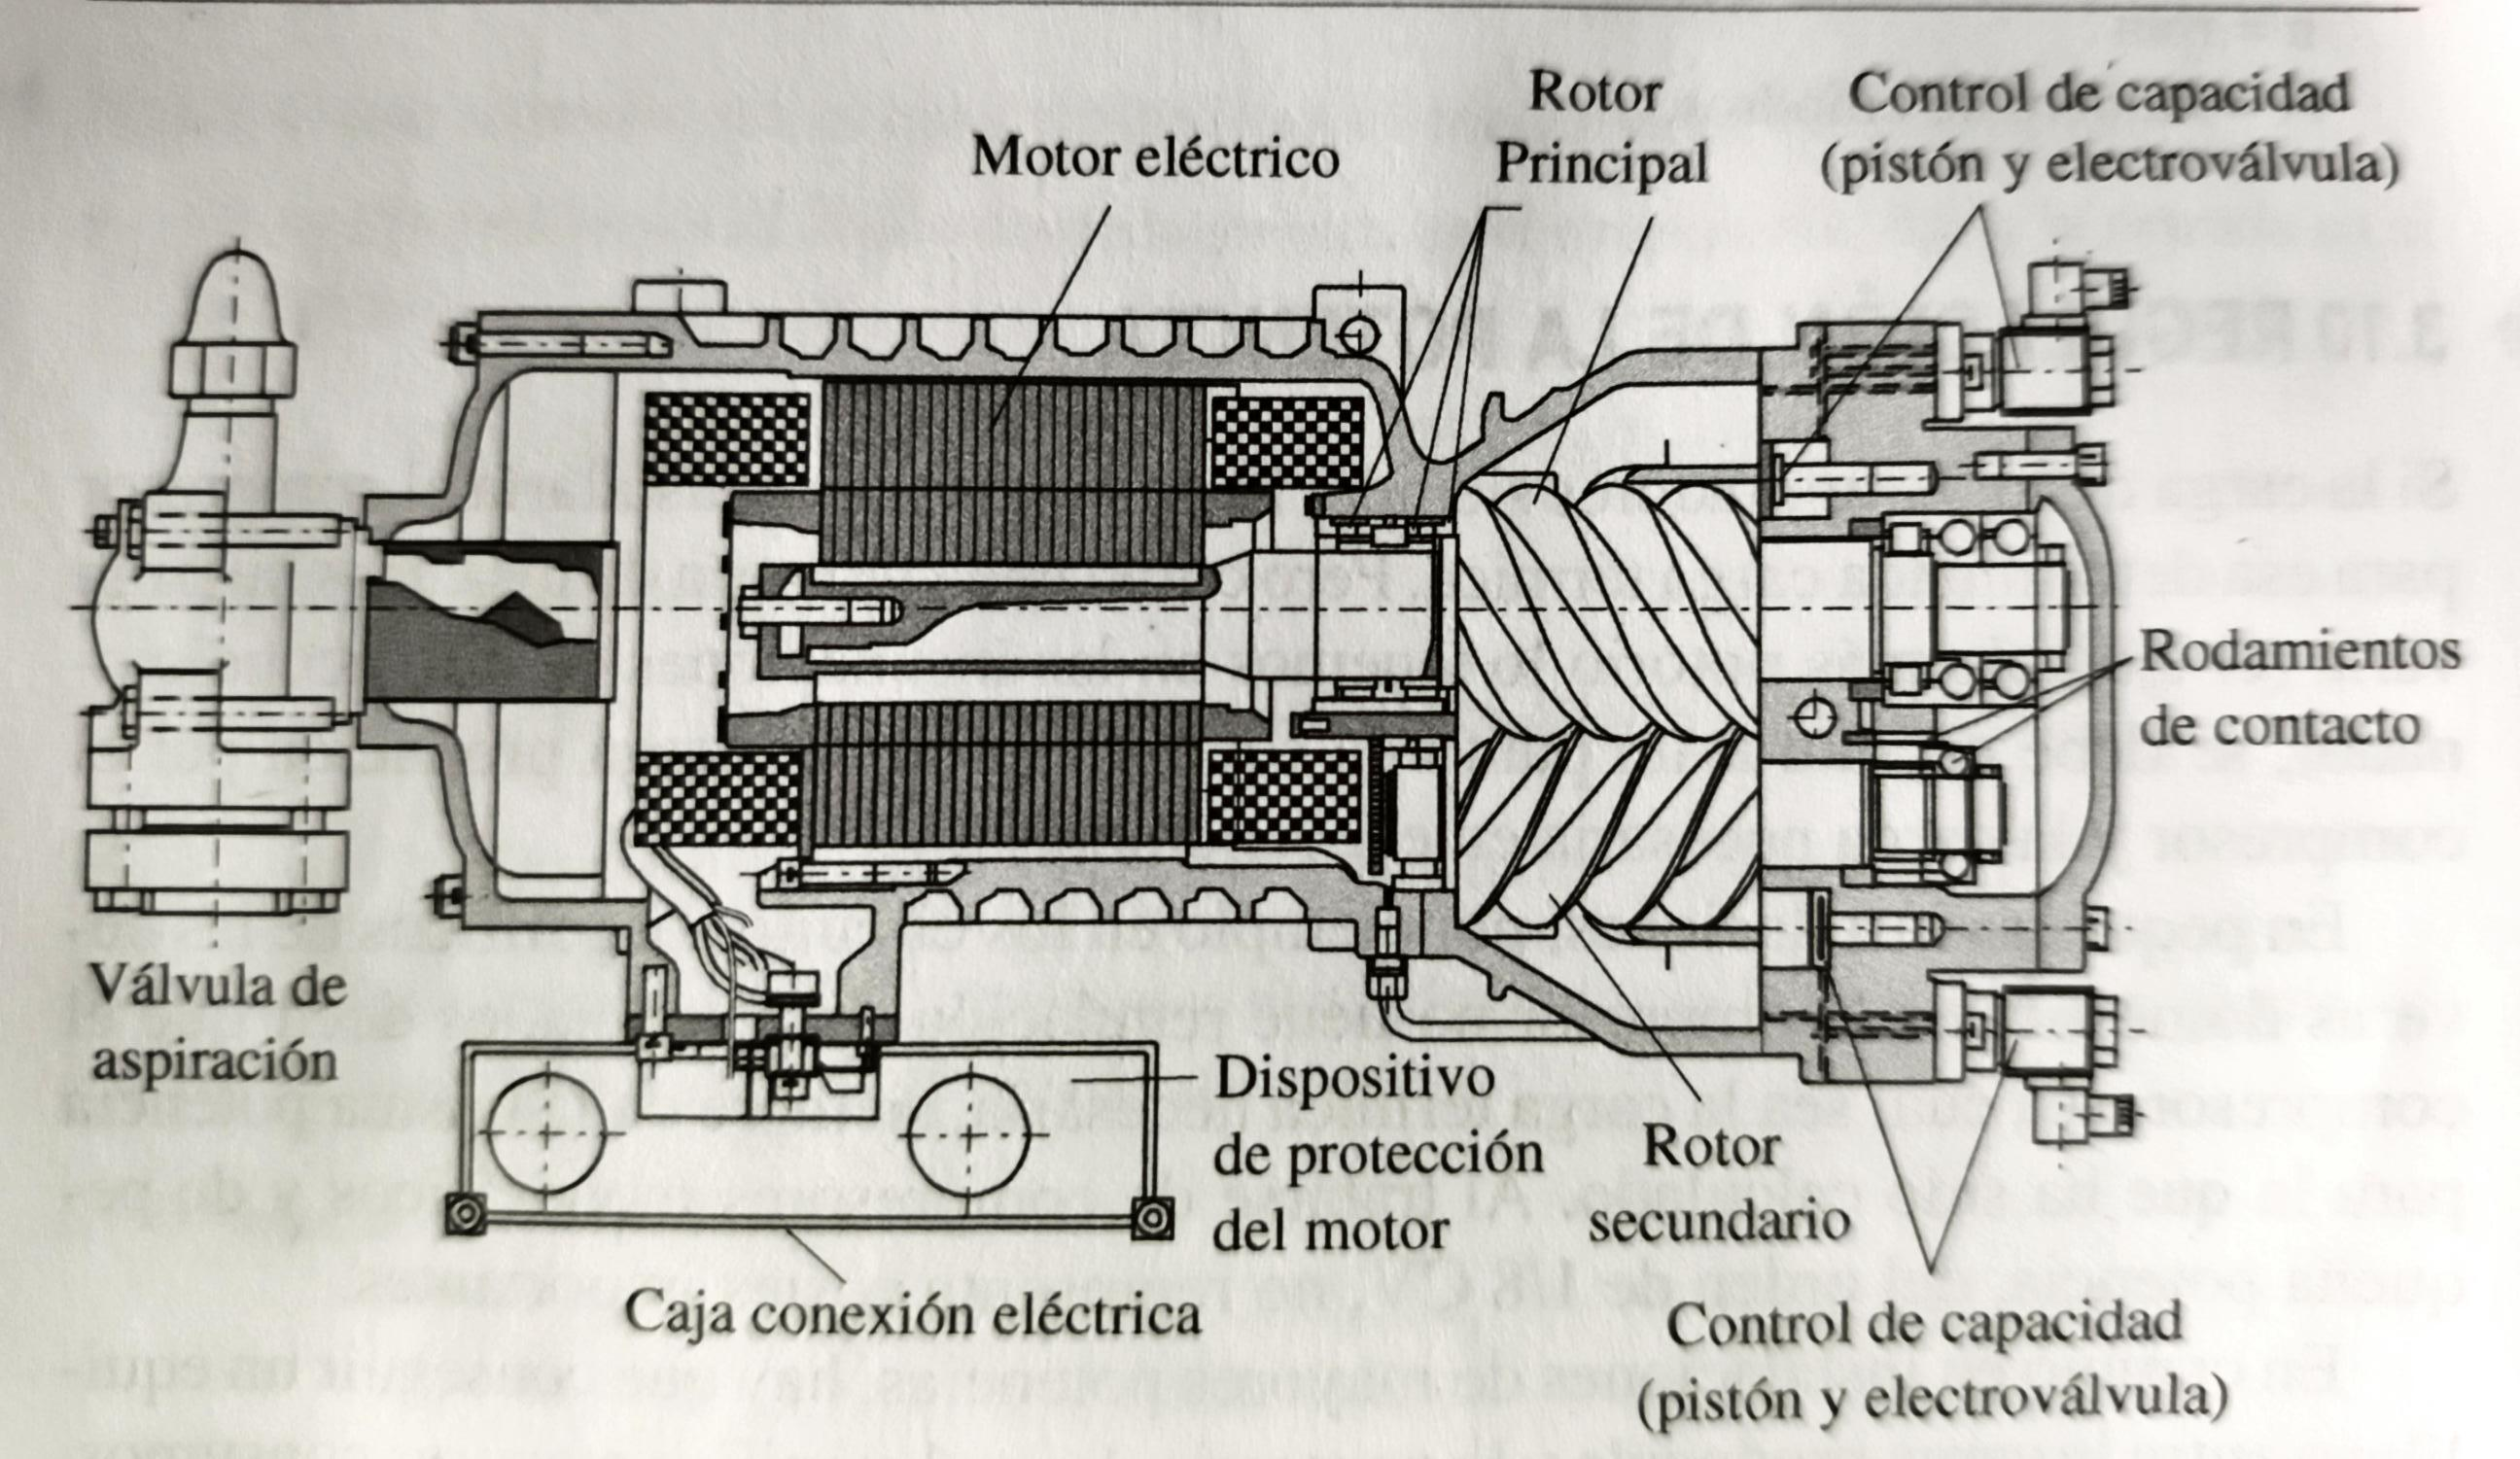
\includegraphics[width=\textwidth]{figuras/compresores/controles de capacidad.jpg}
	\caption{Disposici\'on de los controles de capacidad}
	\label{fig:Disposici\'on de los controles de capacidad}
\end{figure}

\begin{wrapfigure}{r}{0.5\linewidth}
	\centering
	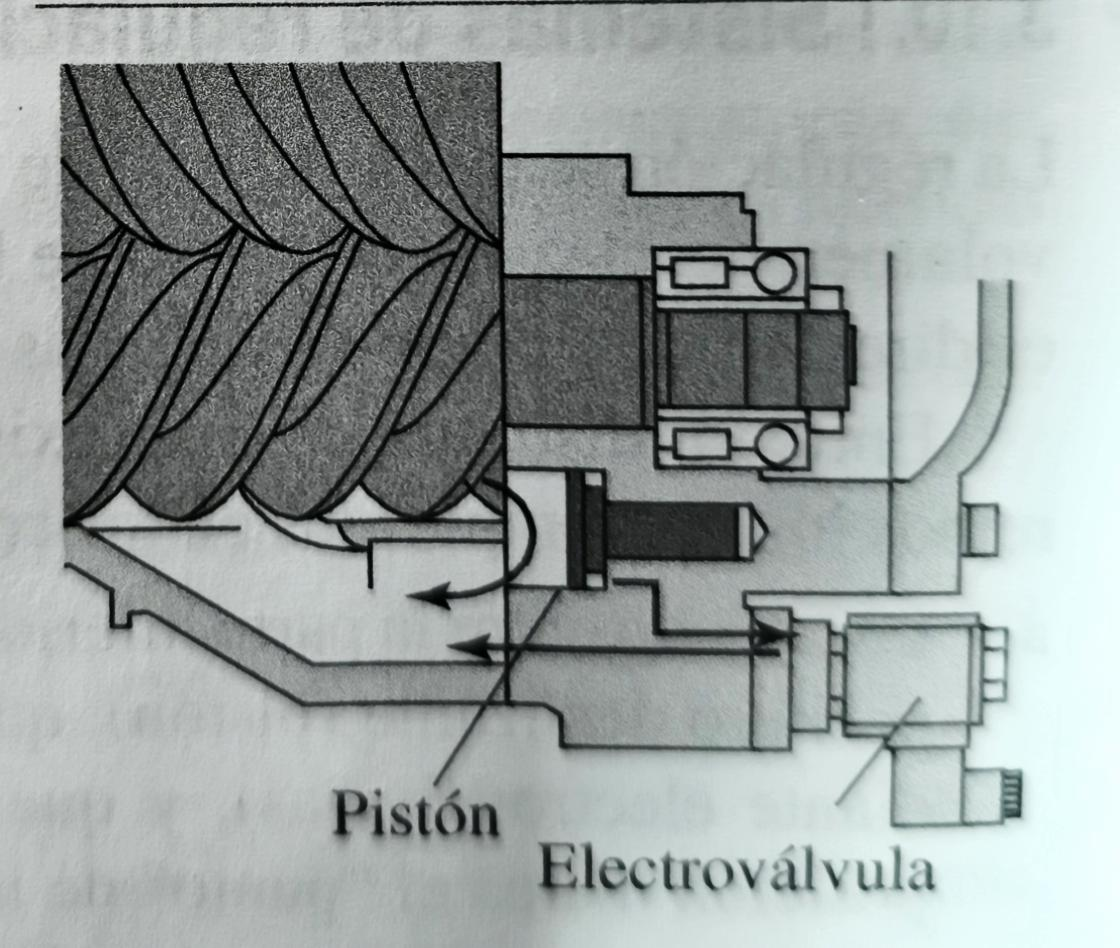
\includegraphics[width=.7\linewidth]{figuras/compresores/detalle de control de capacidad.jpg}
	\caption{Detalle de control de capacidad}
	\label{fig:Detalle de control de capacidad}
\end{wrapfigure}

Los dos pistones son accionados hidr\'aulicamente. Mediante una señal el\'ectrica se abren unos orificios debidamente calibrados, y as\'i una parte del fluido es conducido hacia el lado de la aspiraci\'on (en la \autoref{fig:Detalle de control de capacidad} se aprecia en detalle la operaci\'on)\\Al disminuir el caudal de fluido descargado, tambi\'en se disminuye la potencia. En este sistema, la regulaci\'on de potencia se realiza en dos etapas. Cuando una electrov\'alvula no \'esta activada, se produce una reducci\'on de potencia.

\subsection{Variaciones de las presiones y su repercursión en las potencias}

La potencia frigor\'ifica de un compresor dependen de las condiciones de trabajo. Por ello vamos a ver de que manera repercuten en la potencia frigor\'ifica las variaciones de las presiones de trabajo.\\ En el diagrama de Mollier podemos apreciar c\'omo var\'ia la potencia frigor\'ifica seg\'un las distintas temperaturas de evaporaci\'on y condensaci\'on.
% \renewcommand{\theenumi}{\alph{enumi}}
\begin{enumerate}[a.]
	\item ¿Qu\'e ocurre cuando la presi\'on de aspiraci\'on disminuye?\\ Supongamos que la presi\'on de aspiraci\'on $Pa$, disminuye hasta un valor $Pa^\prime$\\Se comprueba que:
	\begin{enumerate}[1.]
		\item Al disminuir la presi\'on de aspiraci\'on, el efecto refrigerante ($ER^\prime$) tambi\'en disminuye con lo cual disminuye la potencia.
		\item El volumen espec\'ifico ($Ve^\prime$) aumenta, lo que implica que el desplazamiento volum\'etrico disminuye.
	\end{enumerate}

	\begin{figure}[H]
		\centering
		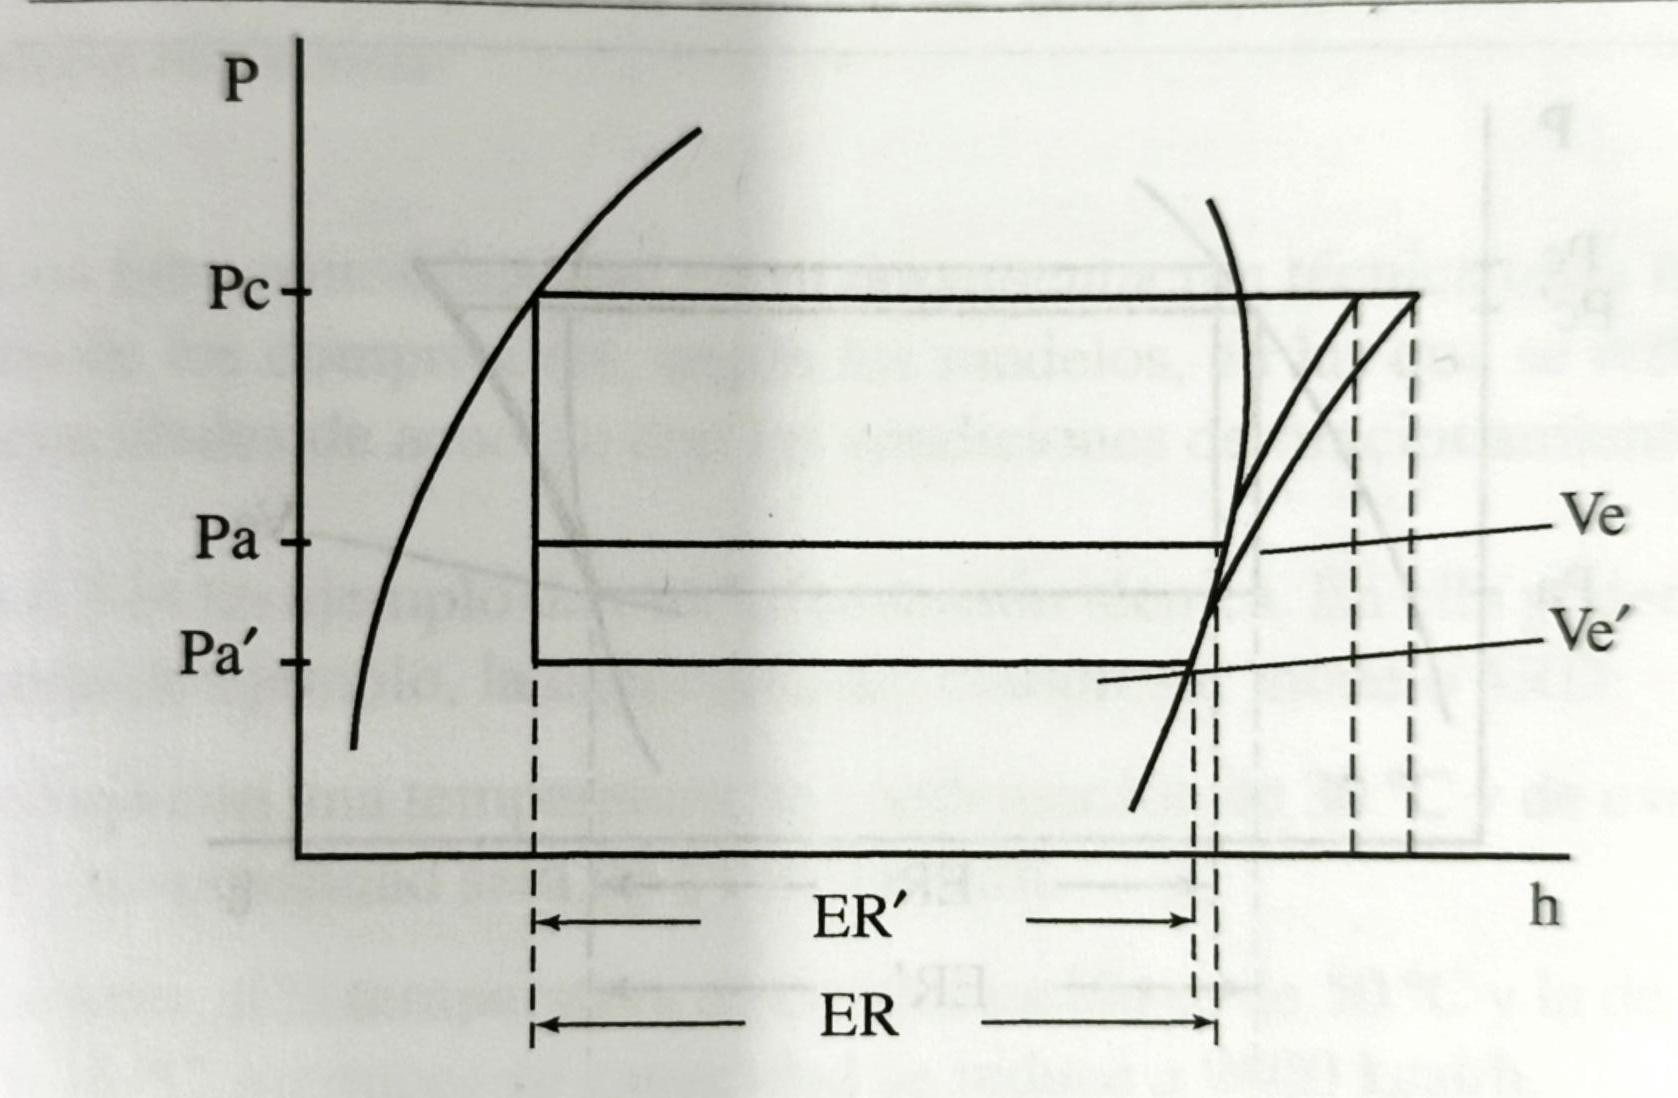
\includegraphics[width=.6\textwidth]{figuras/compresores/variacion de la presion de aspiracion.jpg}
		\caption{Variaci\'on de la psei\'on de aspiraci\'on en el diagrama p-h.}
		\label{Variaci\'on de la presi\'on de aspiraci\'on}
	\end{figure}
	Tambi\'en se puede demostrar num\'ericamente con la relaci\'on de compresi\'on (Rc) para este caso aumenta, por tanto disminuye el rendimiento volum\'etrico (Rv) y la potencia frigor\'ifica.

	\item ¿Qu\'e ocurre con la potencia frigor\'ifica cuando disminuye la presi\'on de condensaci\'on?\\Viendo la \autoref{fig:Variaci\'on de la presi\'on de condensaci\'on} se puede ver que:
	\begin{enumerate}[1.]
		\item El efecto refrigerante ($ER^\prime$) aumenta, con lo que la potencia frigor\'ifica tambi\'en aumenta.
		\item La relaci\'on de compresi\'on (Rc) disminuye, con lo que la potencia frigor\'ifica aumenta.
	\end{enumerate}
	\begin{figure}[H]
		\centering
		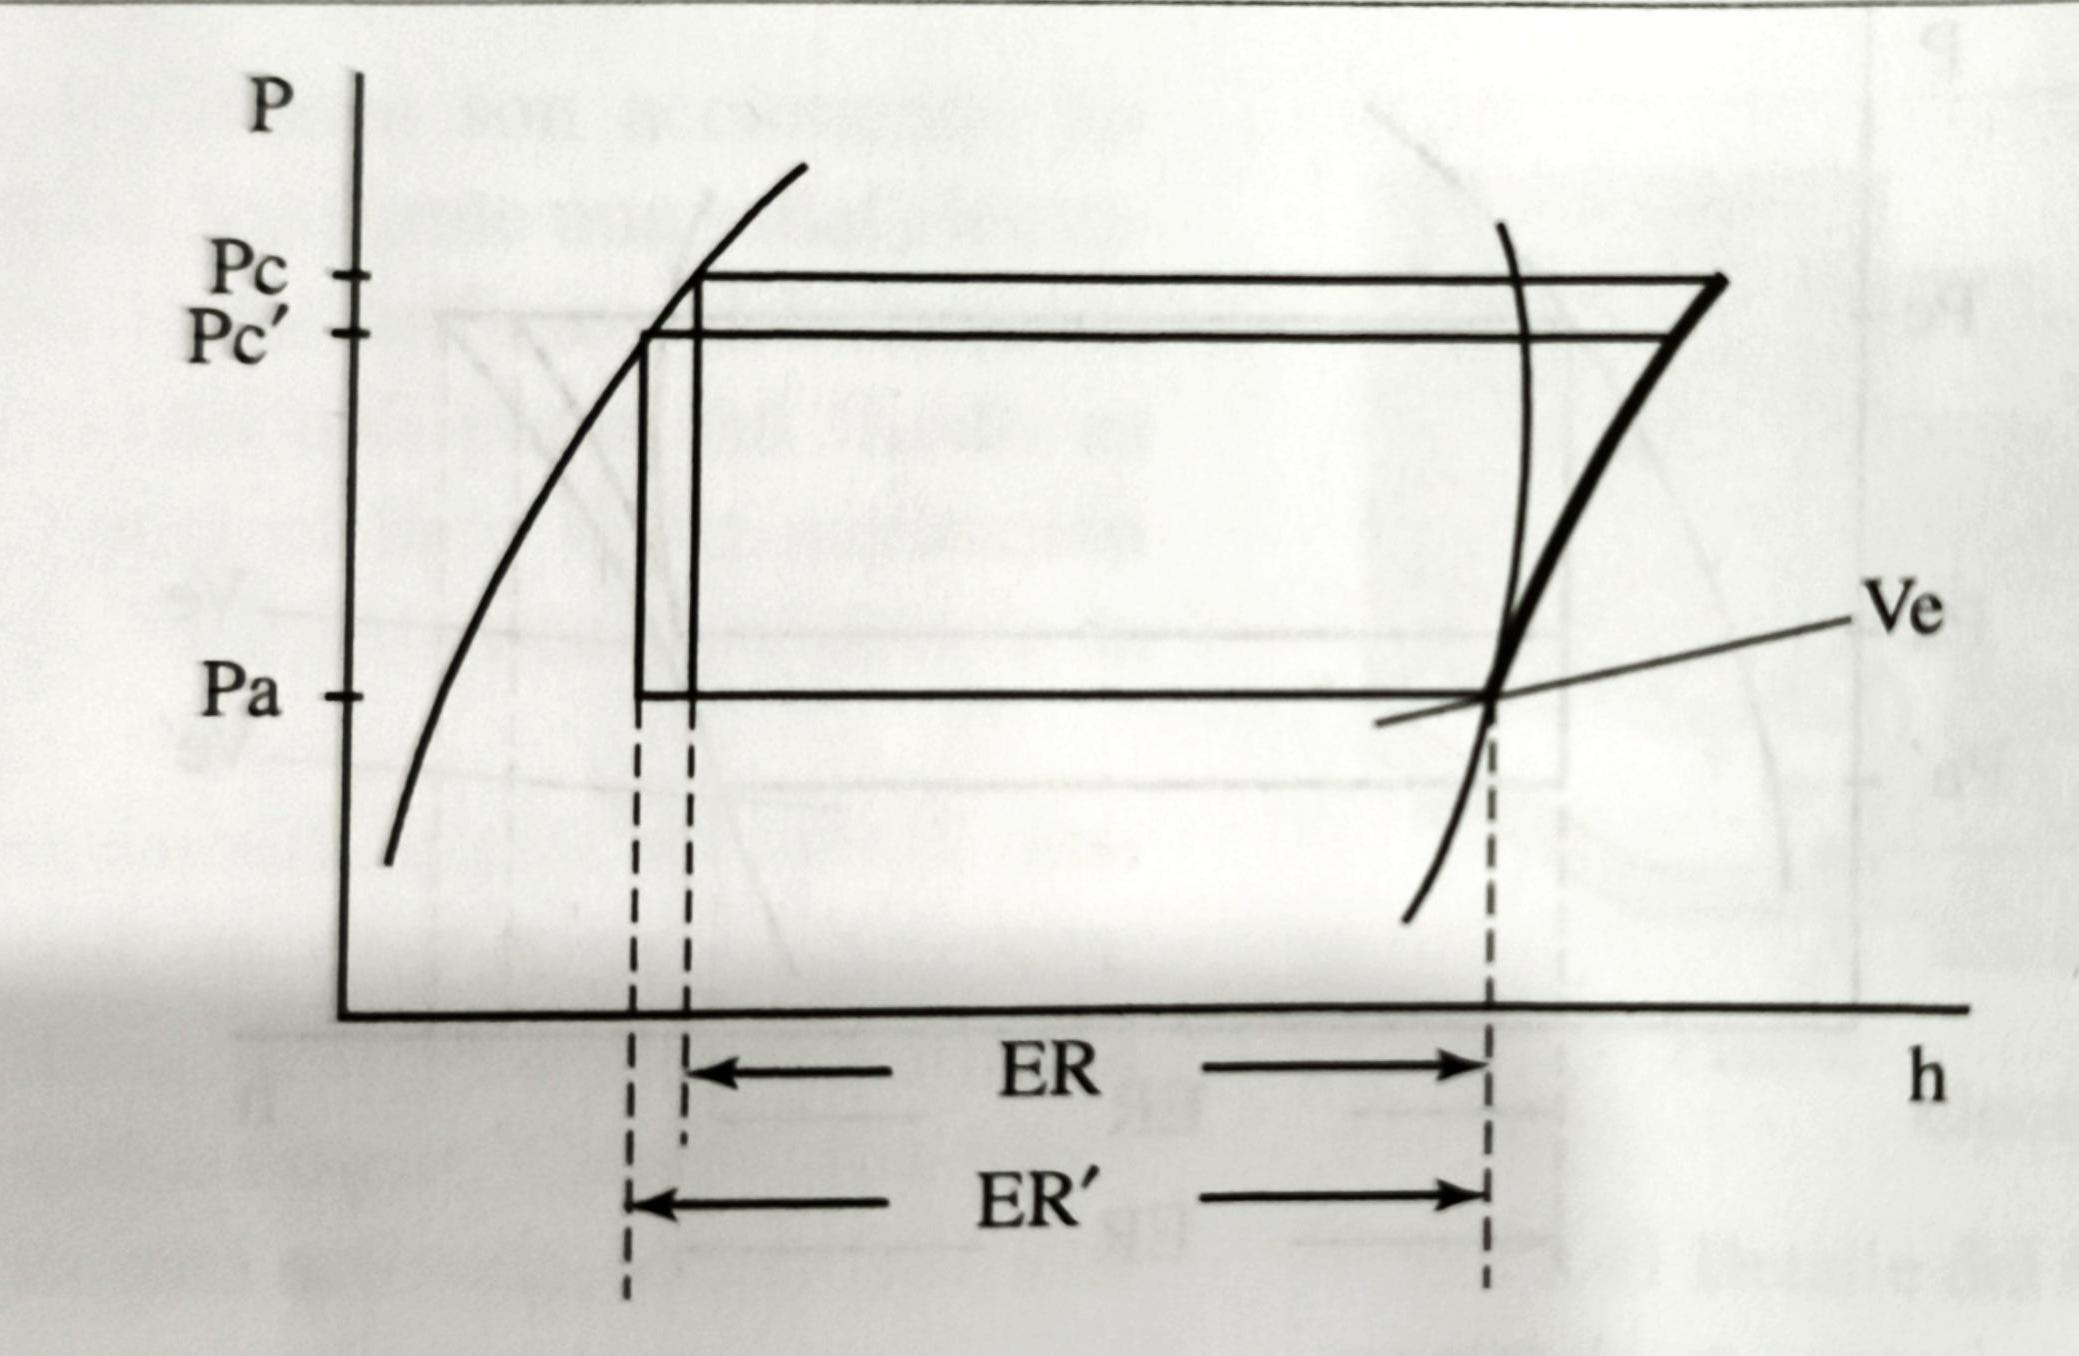
\includegraphics[width=.6\textwidth]{figuras/compresores/variacion de la presion de condensacion.jpg}
		\caption{Variaci\'on de la presi\'on de condensaci\'on en el diagrama p-h}
		\label{fig:Variaci\'on de la presi\'on de condensaci\'on}
	\end{figure}
\end{enumerate}
La \autoref{fig:Capacidad de un compresor modelo 4RD} es un ejemplo es informaci\'on t\'ecnica de un compresor modelo 4RD, en ella podemos corroborar lo anteriormente dicho:
\begin{enumerate}[a.]
	\item Si la temperatura de condensaci\'on es 30\textcelsius\ y de evaporaci\'on -5\textcelsius, entonces su capacidad ser\'a de 11800 kcal/h.
	\item En cambio, si la temperatura de condensaci\'on es de 50\textcelsius\ y la de evaporaci\'on es de -5\textcelsius, entonces su capacidad se reduce a 9400 kcal/h.
\end{enumerate}
\begin{figure}[h]
	\centering
	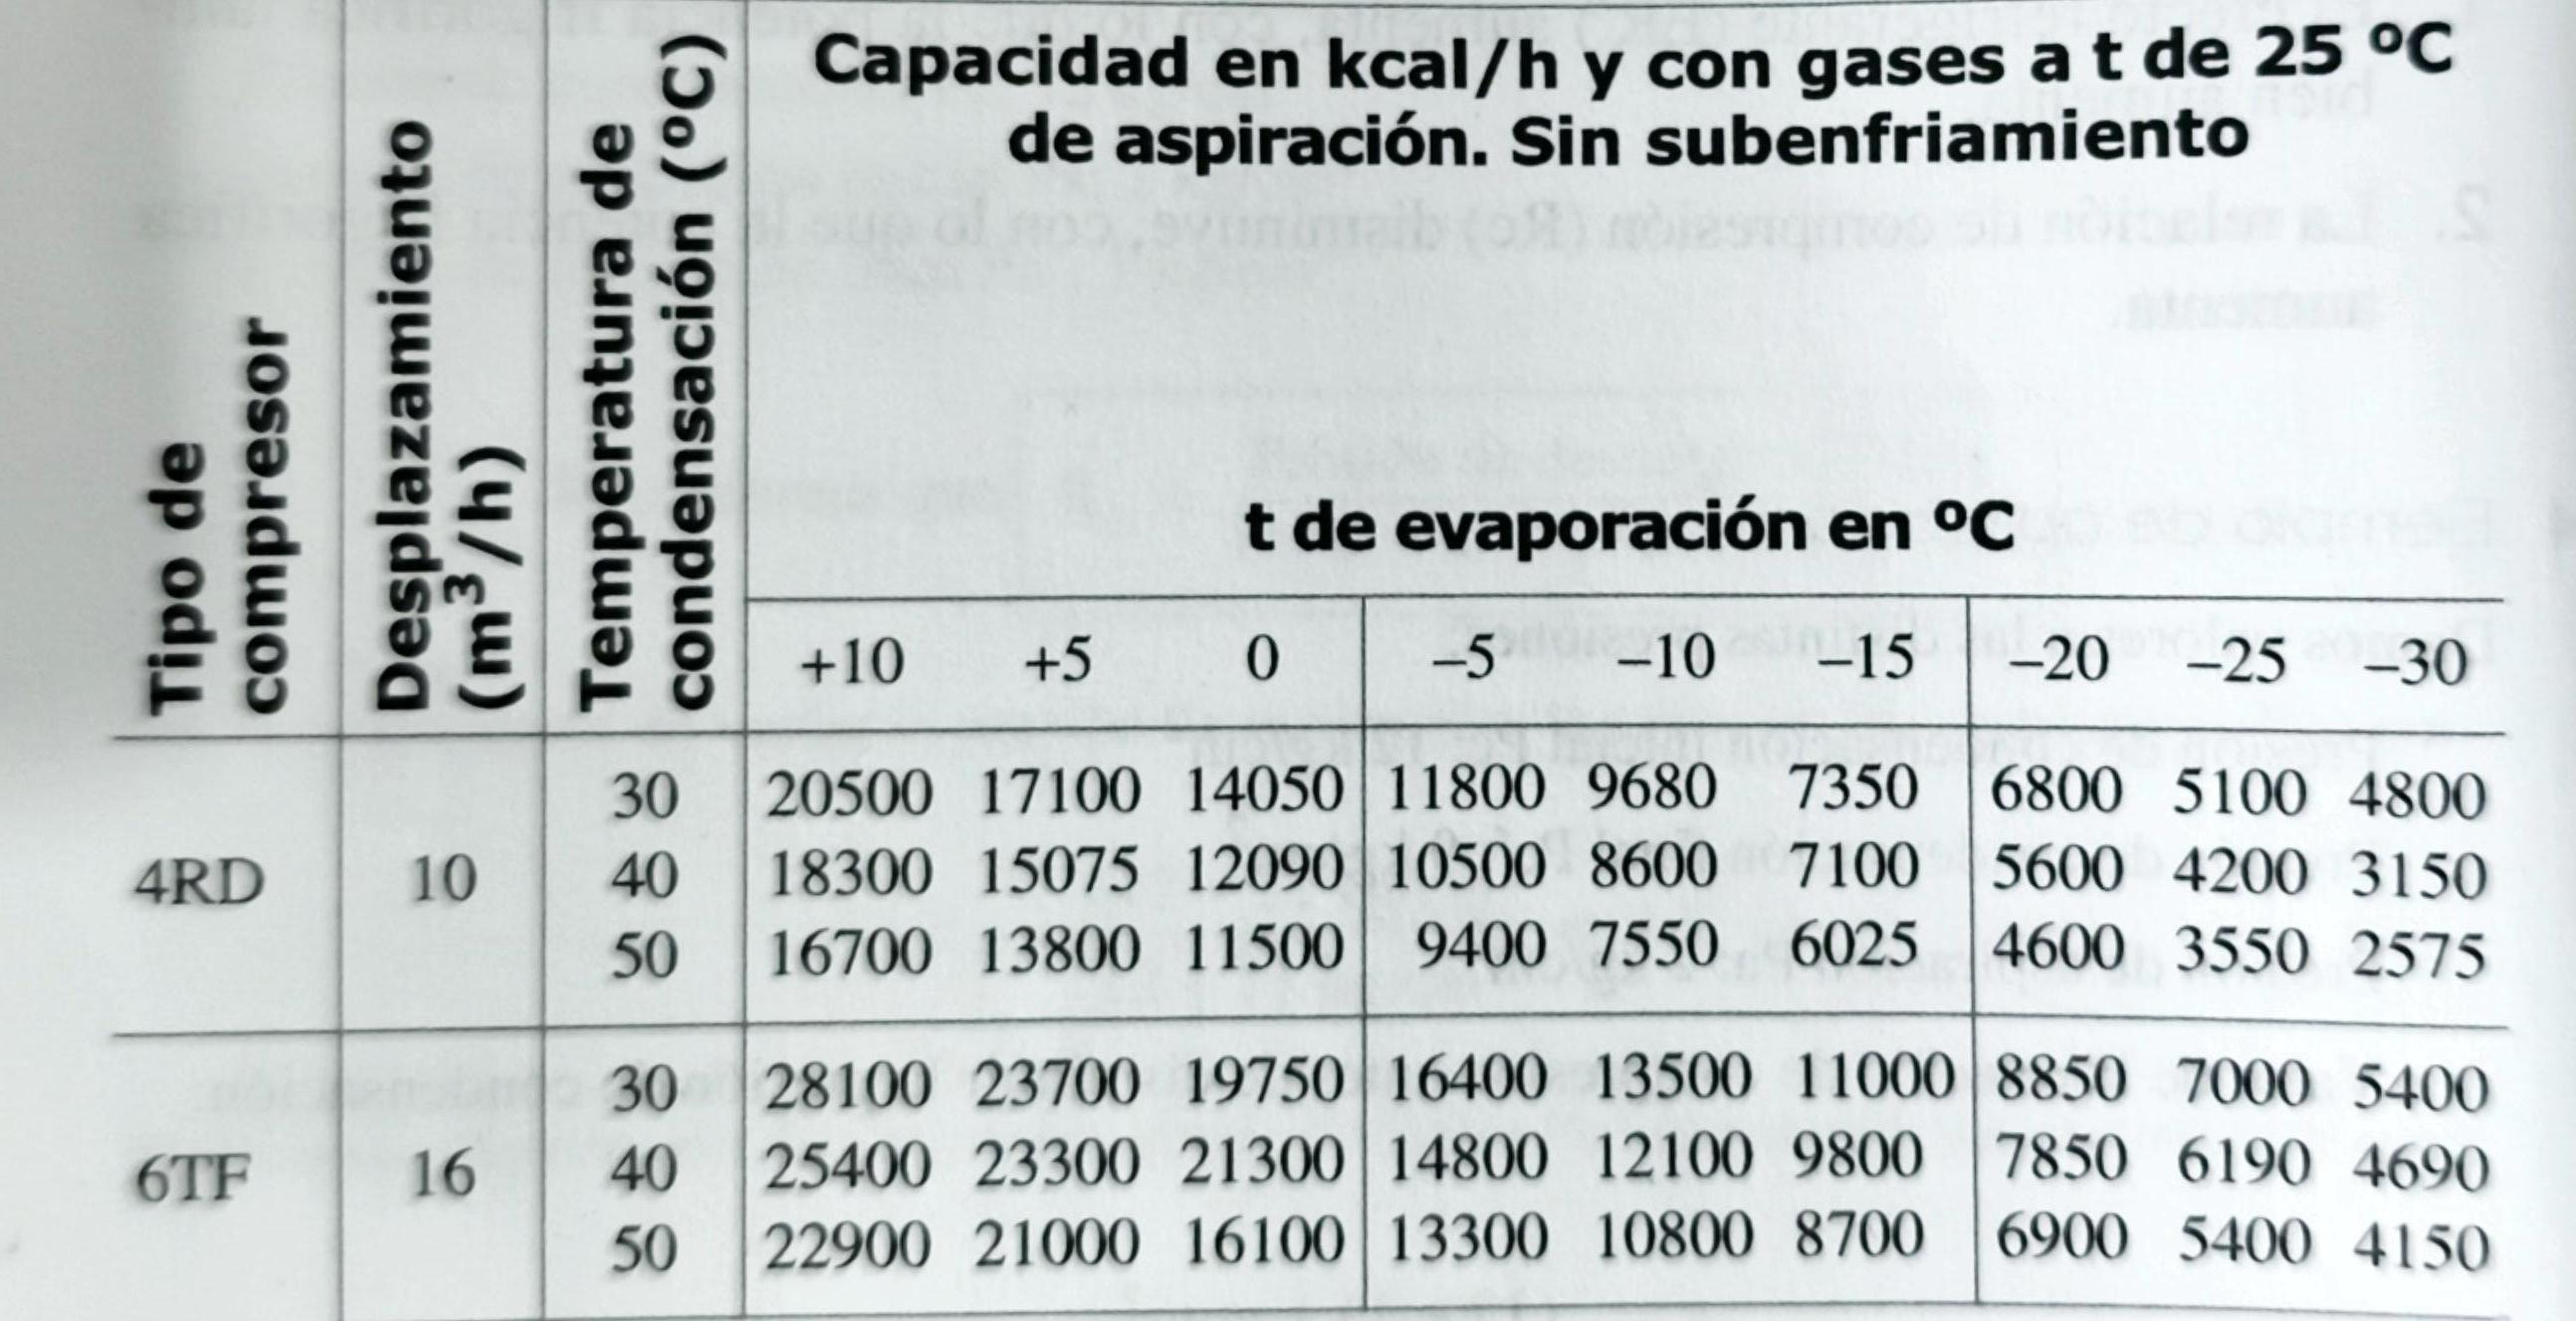
\includegraphics[width=\linewidth]{figuras/compresores/tabla de capacidad de un compresor.jpg}
	\caption{Capacidad de un compresor modelo 4RD}
	\label{fig:Capacidad de un compresor modelo 4RD}
\end{figure}
\subsection{Funcionamiento en régimen seco y en régimen húmedo}
Se dice que trabaja en \textsl{r\'egimen h\'umedo} cuando el fluido a la entrada del compresor es una mezcla de gas y l\'iquido (Tramo 1-2 de la \autoref{fig:R\'egimen seco y h\'umedo}). Esto puede ocurrir por diversas causas, tales como:
\begin{enumerate}[a.]
	\item Mala regulaci\'on del dispositivo de expansi\'on y entra demasiado fluido refrigerante en el evaporador.
	\item Mala circulaci\'on del aire a trav\'es del evaporador por obstrucci\'on o por caudal insuficiente.
\end{enumerate}
Pero en esa mezcla, la cantidad de l\'iquido a\'un no es lo suficiente importante para producir el golpe de l\'iquido, ya que se va evaporando debido a las temperaturas m\'as altas que se va encontrando, por ejemplo:
\begin{enumerate}[a.]
	\item En la conexi\'on tuber\'ia de aspiraci\'on-compresor
	\item En la culata
	\item En el pist\'on
	\item En la camisa
	\item Durante la fase de compresi\'on 
\end{enumerate}

\begin{wrapfigure}{r}{0.5\linewidth}
	\centering
	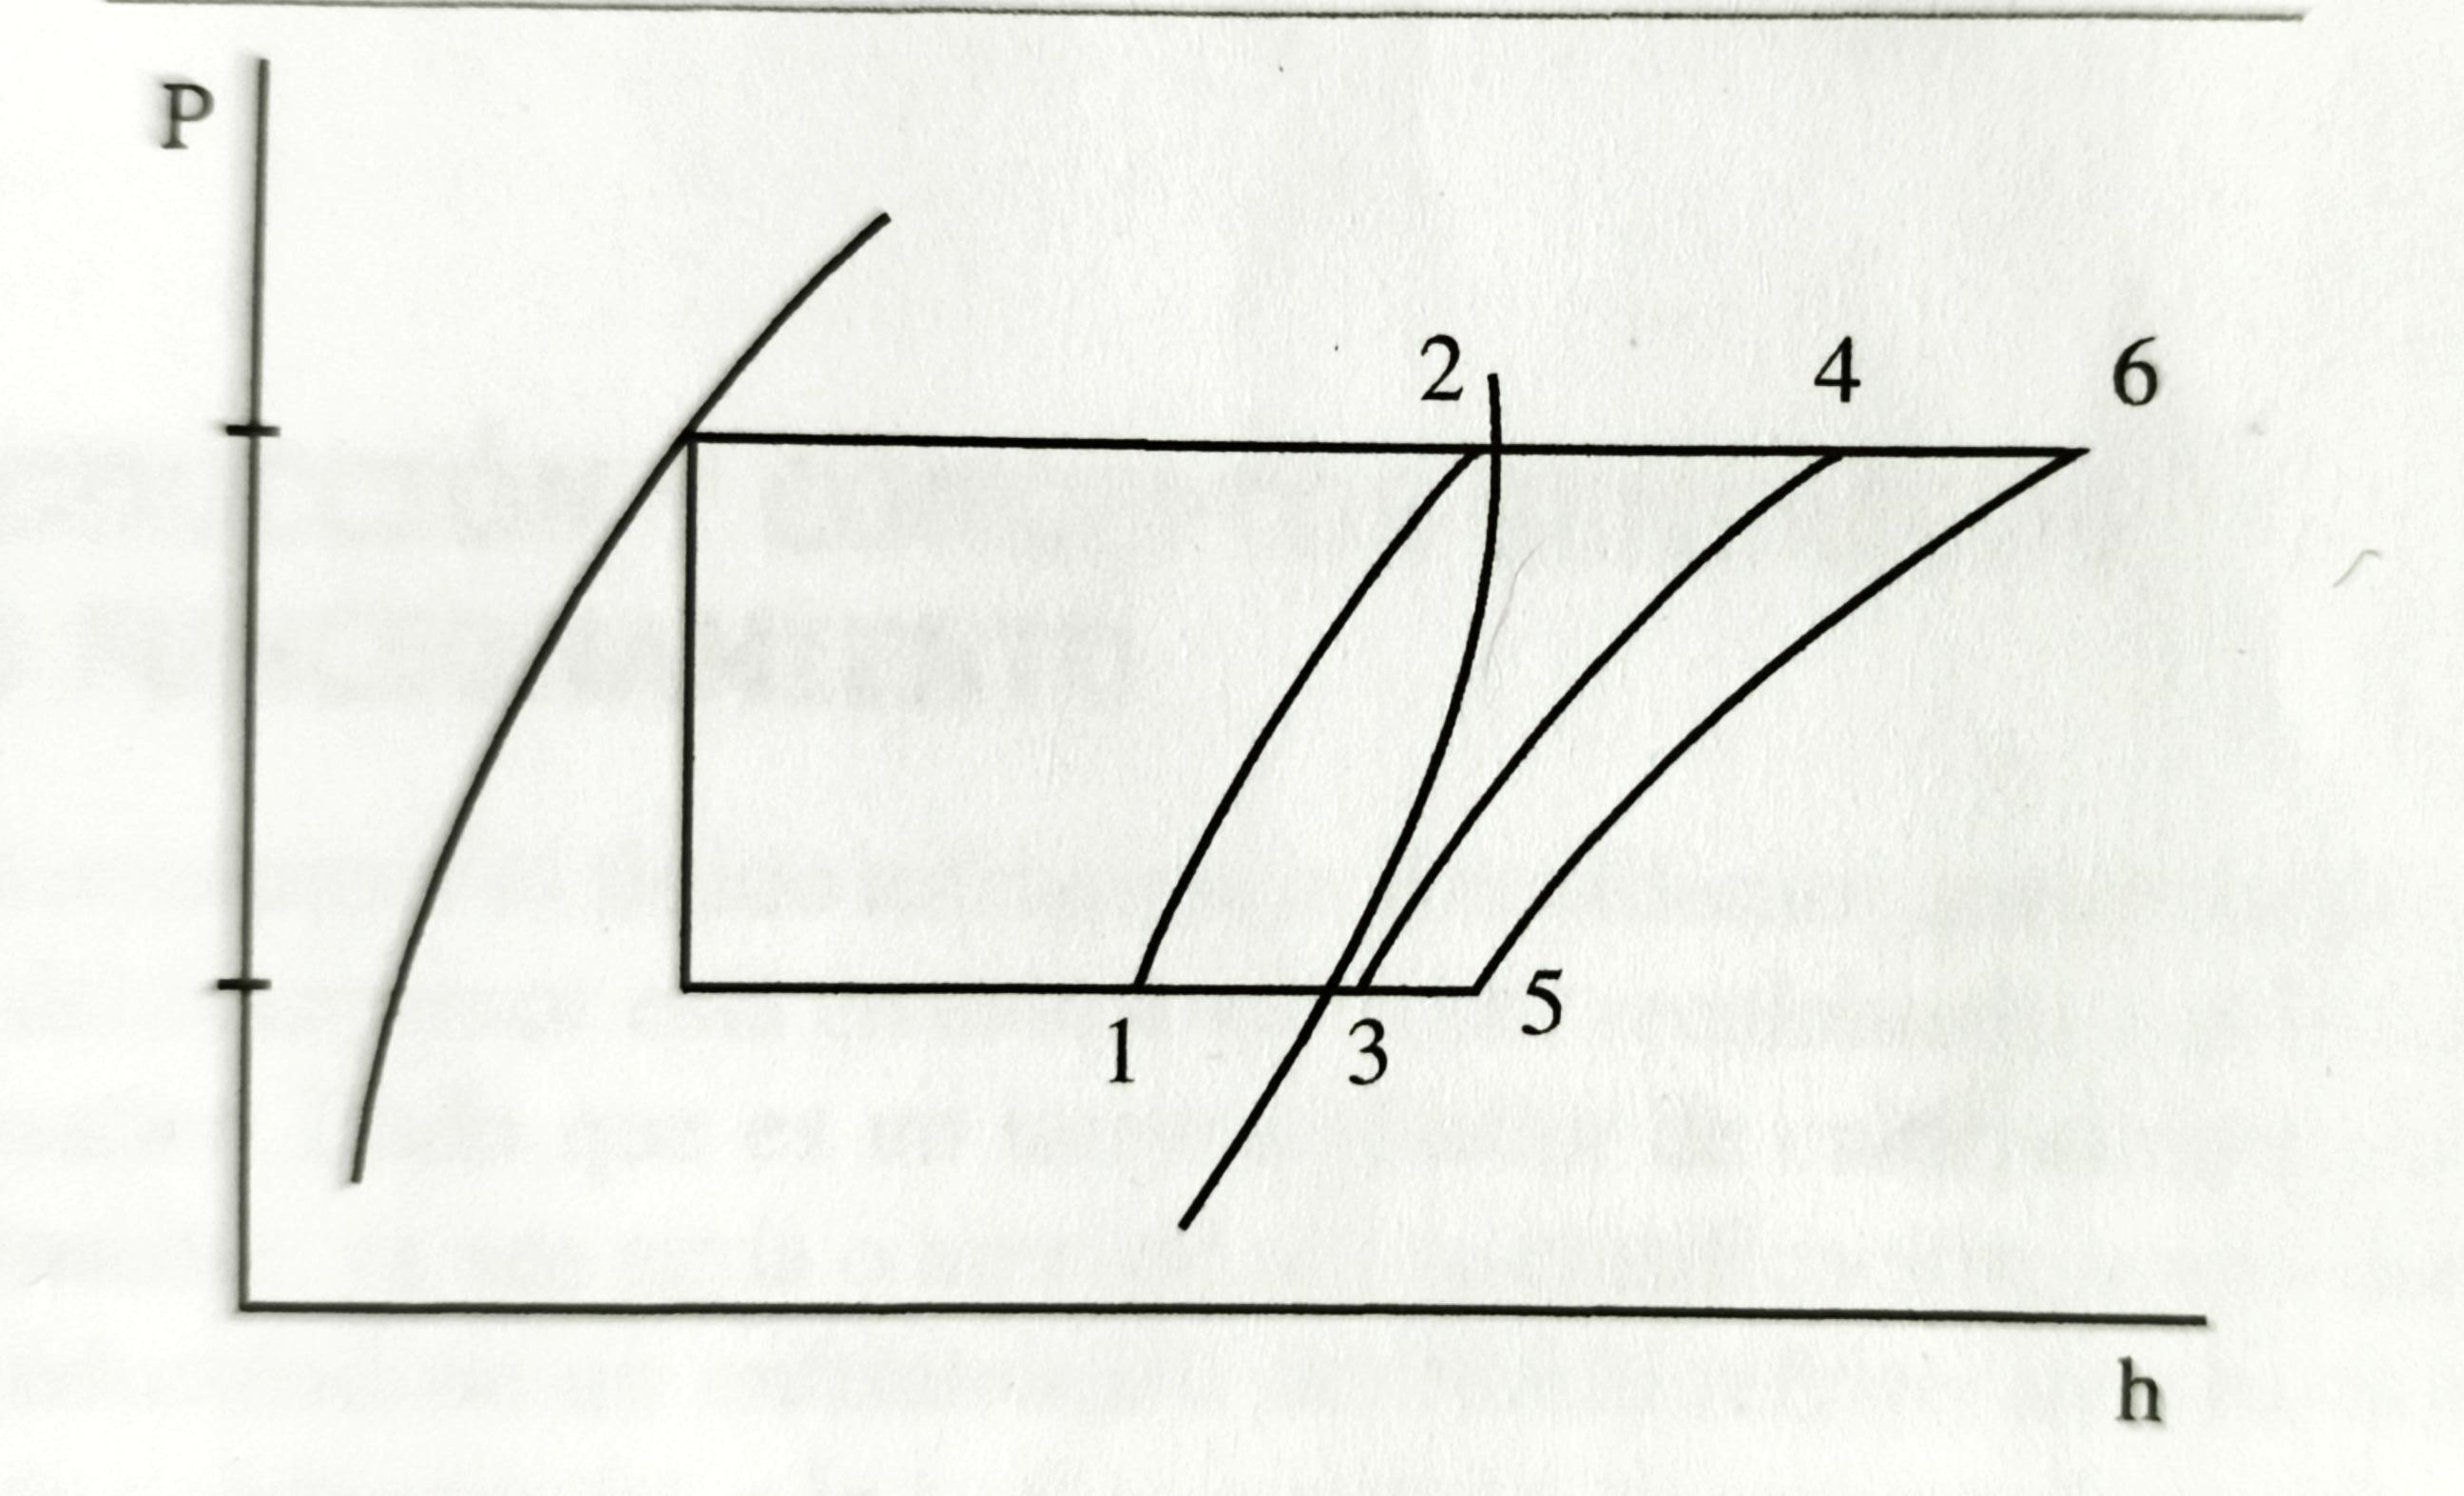
\includegraphics[width=.8\linewidth]{figuras/compresores/régimen seco y humedo.jpg}
	\caption{R\'egimen seco y h\'umedo}
	\label{fig:R\'egimen seco y h\'umedo}
\end{wrapfigure}

Pero ese calor que absorbe el l\'iquido lo est\'a haciendo del calor proveniente del compresor e instalaci\'on y no del ambiente a refrigerar (en el evaporador).\\ En cambio, cuando el fluido a la entrada del compresor es vapor (Tramo 3-4 de la \autoref{fig:R\'egimen seco y h\'umedo}), entonces se trata del \textbf{r\'egimen seco} y, en este caso, el rendimiento es mayor que en el caso anterior. Pero se debe tener especial cuidado para este tipo de funcionamiento, ya que si el vapor que entra al compresor est\'a demasiado sobrecalentado puede generar temperaturas de descarga elevadas por lo que el rendimiento del ciclo ser\'a perjudicado (Tramo 5-6 de la \autoref{fig:R\'egimen seco y h\'umedo}).		


		\section{Compresores}

Es el coraz\'on de la instalaci\'on. Su funci\'on, dentro del sistema de refrigeración, consiste en aspirar el fluido refrigerante a baja presi\'on y temperatura tales que se pueda condensar.

Lo escrito en esta secci\'on esta basado en el libro \textit{Manual de refrigeración} de \cite[cap\'itulo 3]{Franco2016Manual}.

Los tipos de compresores m\'as empleados en la refrigeración son:

\begin{itemize}
	\item Alternativos 
	\item De tornillo o helicoidales
	\item Rotativos
	\item Centr\'ifugos
\end{itemize}

\subsection{Alternativos}

Pueden ser de simple efecto o de doble efecto, seg\'un realice la compresi\'on del fluido en un solo lado del pist\'on o en ambos lados. Los m\'as utilizados son los de simple efecto.

\subsubsection{Elementos del compresor}

\textbf{Bloque}

El bloque aglutina y soporta todos los elementos del compresor, tanto como fijos como m\'oviles. La parte superior es la culata y la inferior, por su interior, el c\'arter.

\begin{figure}[H]
	\centering
	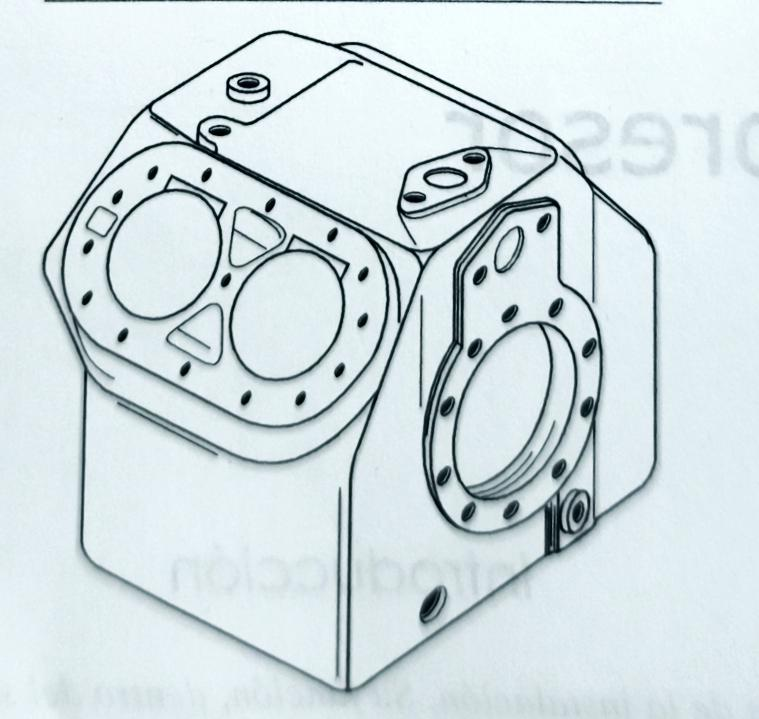
\includegraphics[width=.5\linewidth]{figuras/compresores/bloque}
	\caption{Bloque de un compresor}
	\label{fig:Bloque de un compresor}
\end{figure}

\textbf{C\'arter}

Es el espacio interior comprendido entre el eje cig\"ue\~{n}al y el fondo del bloque, destinado a almacenar el aceite de lubricación.

\textbf{Cilindro}
\begin{wrapfigure}{r}{0.4\linewidth}
	\centering
	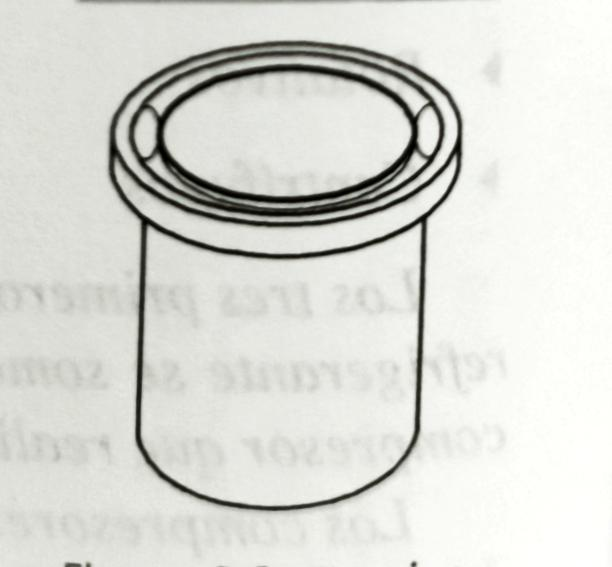
\includegraphics[width=.5\linewidth]{figuras/compresores/cilindro con camisa.jpg}
	\caption{Camisa}
	\label{fig:Camisa}
\end{wrapfigure}
Espacio donde va alojado el pist\'on. En su interior, \'este se desplaza en movimiento rect\'ilineo alternativo. En compresores de mediana y gran potencia (\autoref{fig:Camisa}) lleva camisa, que es una pieza cil\'indrica de acero que lo reviste, y que en casos de desgaste se puede rectificar, o sustituir si procede.

\textbf{Pist\'on o \'embolo}

Elemento que,desplaz\'andose en el interior del cilindro, provoca la aspiraci\'on, compresión y descarga del fluido refrigerante. Lleva alojados los aros o segmentos, que pueden ser:
\begin{itemize}
	\item Aros de engrase: Permiten la lubricación de los cilindros y, en su movimiento, arrastran el aceite al c\'arter.
	\item Aros de compresi\'on: Impiden que el fluido refrigerante escape por los espacios entre el pist\'on y el cilindro, hacia la parte inferior (c\'arter). Esto se aprecia mejor durante la compresi\'on, ya que si hay fugas no se alcanzan las altas presiones necesarias.
\end{itemize}
\textbf{Biela}\\
La biela (\autoref{fig:Conjunto biela-pist\'on y aros}) es el elemento que uno el pist\'on con el eje cig\"ue\~{n}al. Transforma el movimiento circular del eje cig\"ue~{n}al en rectil\'ineo alternativo del pist\'on. Por ello son resistentes y ligeras. La parte superior se llama pie de biela y se une al pist\'on por medio de un bul\'on para evitar el desplazamiento lateral de \'este. Y la parte inferior se llama cabeza de biela y se uno al eje cig\"ue\~{n}al. La biela puede ser de dos tipos, seg\'un se conecte al eje cig\"u\~{n}alo a una exc\'entrica.
\begin{figure}[H]
	\centering
	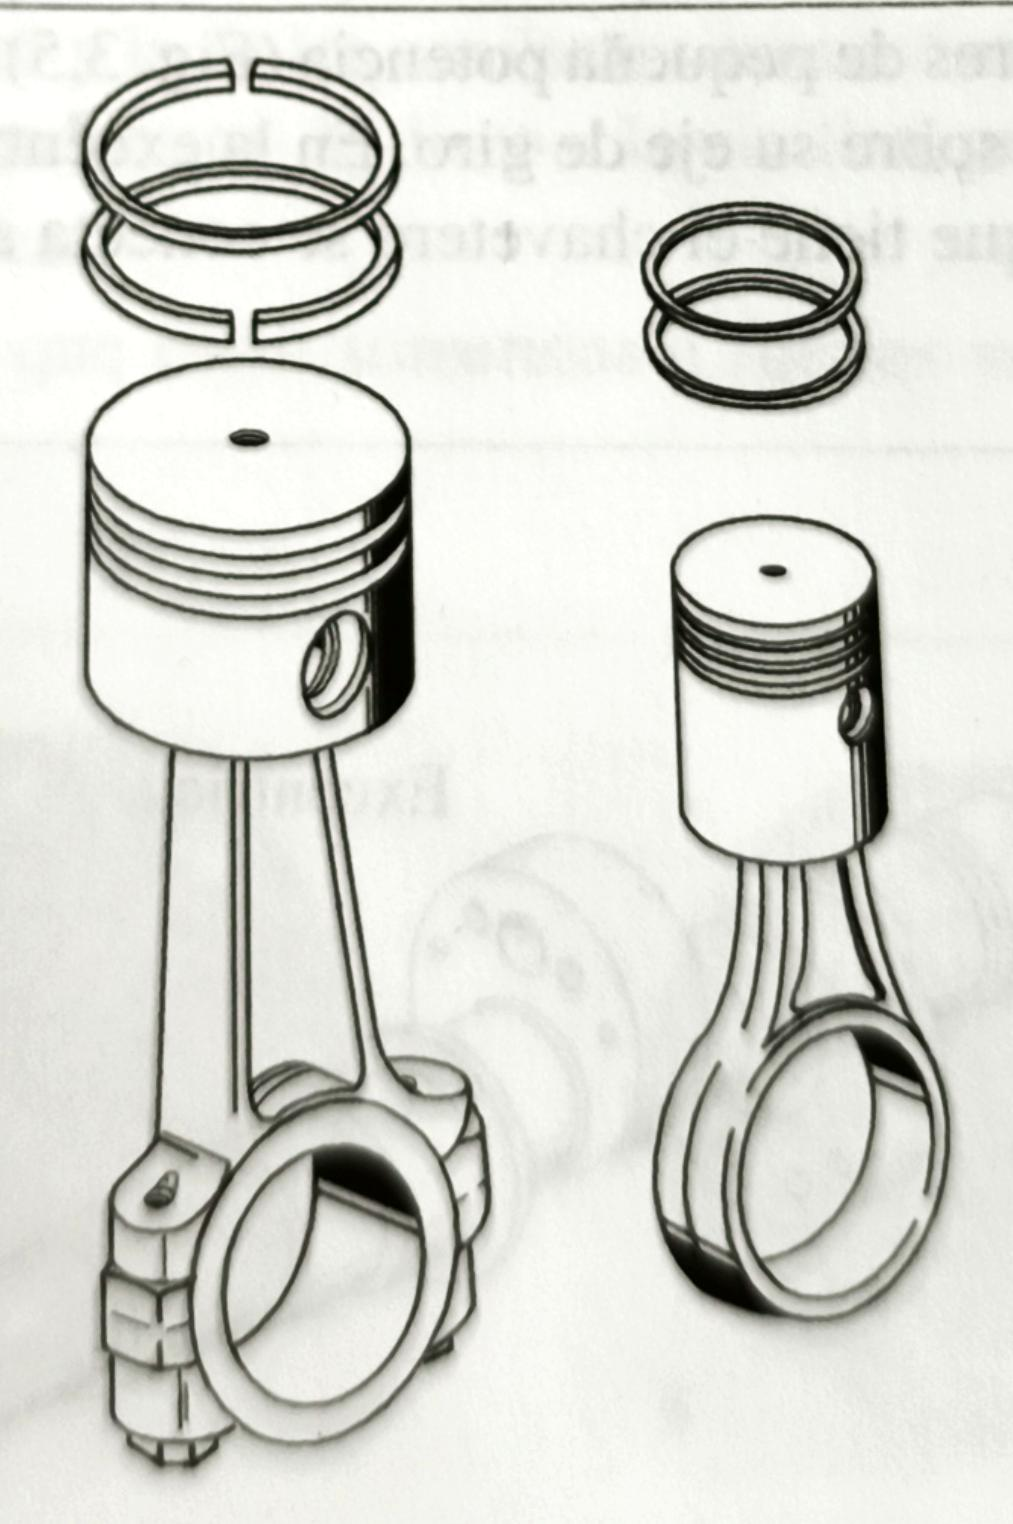
\includegraphics[width=.3\textwidth]{figuras/compresores/piston y biela.jpg}
	\caption{Conjunto biela-pist\'on y aros}
	\label{fig:Conjunto biela-pist\'on y aros}
\end{figure}

\textbf{Eje cig\"ue\~{n}al}\\
La disposici\'on y forma dependen del n\'umero de cilindros (\autoref{fig:Eje cigueñal}). Est\'a formado por un n\'umero determinado de manivelas, que tienen en sus respectivos lados opuestos unos contrapesos de equilibrado. La manivela es la part eque se coencta a la biela.\\
Los extremos del eje, llamados cuellos o mu\~{n}equillas, son los soportes que se apoyan sobe la bancada del compresor. El extremo del eje que tiene el chavetero es el que se conecta al motor el\'ectrico para su accionamiento. El otro extremo acciona la bomba de lubricación.
\begin{figure}[H]
	\centering
	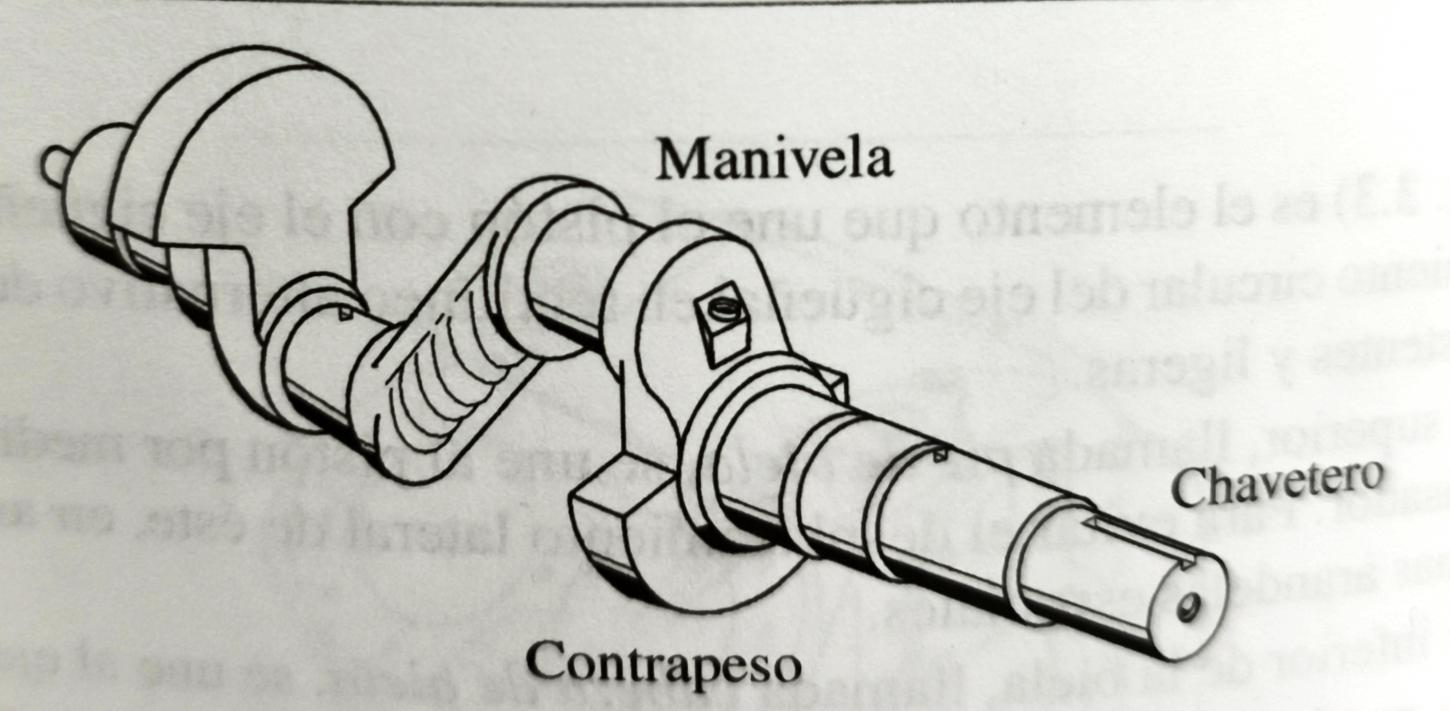
\includegraphics[width=.5\textwidth]{figuras/compresores/eje cigueñal.jpg}
	\caption{Eje cigueñal}
	\label{fig:Eje cigueñal}
\end{figure}
\textbf{Eje de exc\'entrica}\\
Se emplea en compresores de peque\~{n}a potencia (\autoref{fig:Eje de exc\'entrica}). Act\'ua de forma exc\'entrica, de ah\'i el nombre, sobre su eje de giro. En la exc\'entrica se monta la biela. El extremo del eje que tiene el chavetero se conecta al motor el\'ectrico.
\begin{figure}[H]
	\centering
	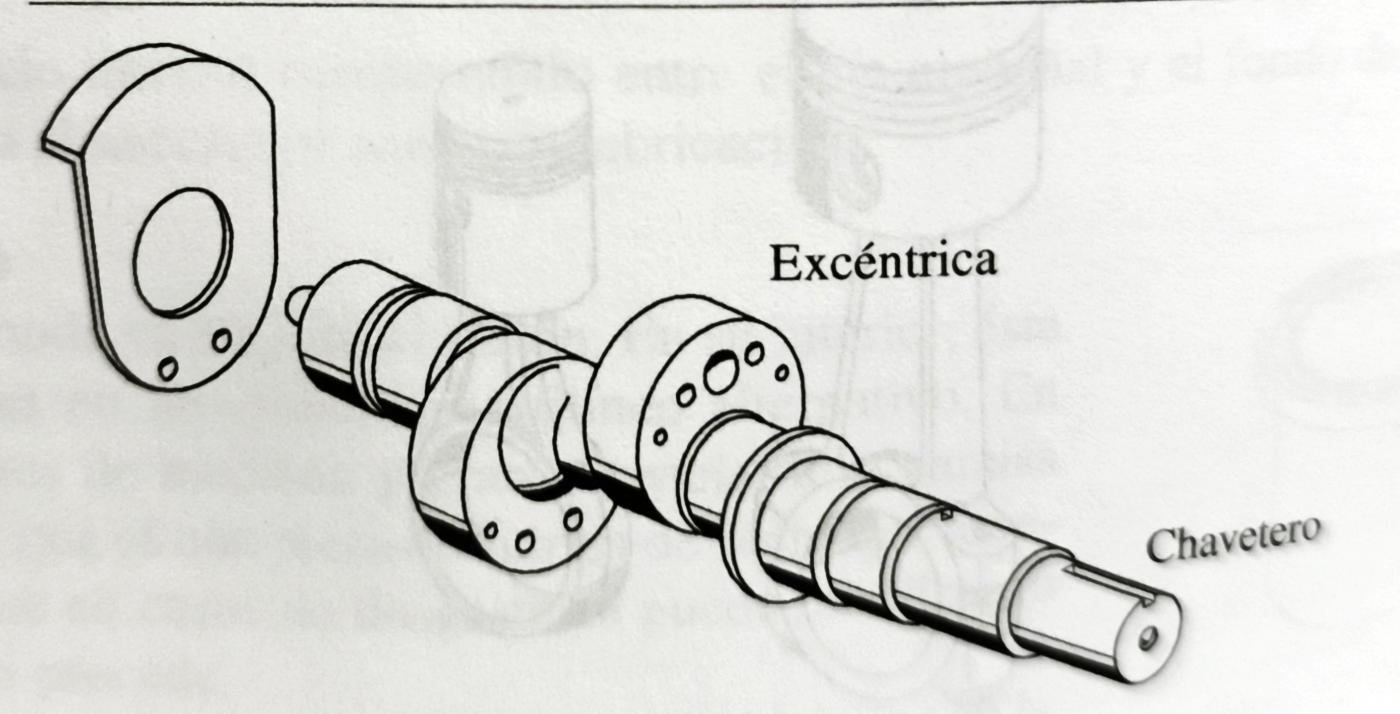
\includegraphics[width=.5\textwidth]{figuras/compresores/eje excentrico.jpg}
	\caption{Eje de exc\'entrica}
	\label{fig:Eje de exc\'entrica}
\end{figure}
\textbf{Culata}\\
Cierra el cilindro por la parte superior. Es la ``tapa'' del cilindro. En ella se alojan las v\'alvulas de aspiración y descarga. Como est\'a sometida a altas temperaturas puede ser refrigerada por aire o por agua (\autoref{fig:Culatas refrigeradas por aire y por agua}).
\begin{figure}[H]
	\centering
	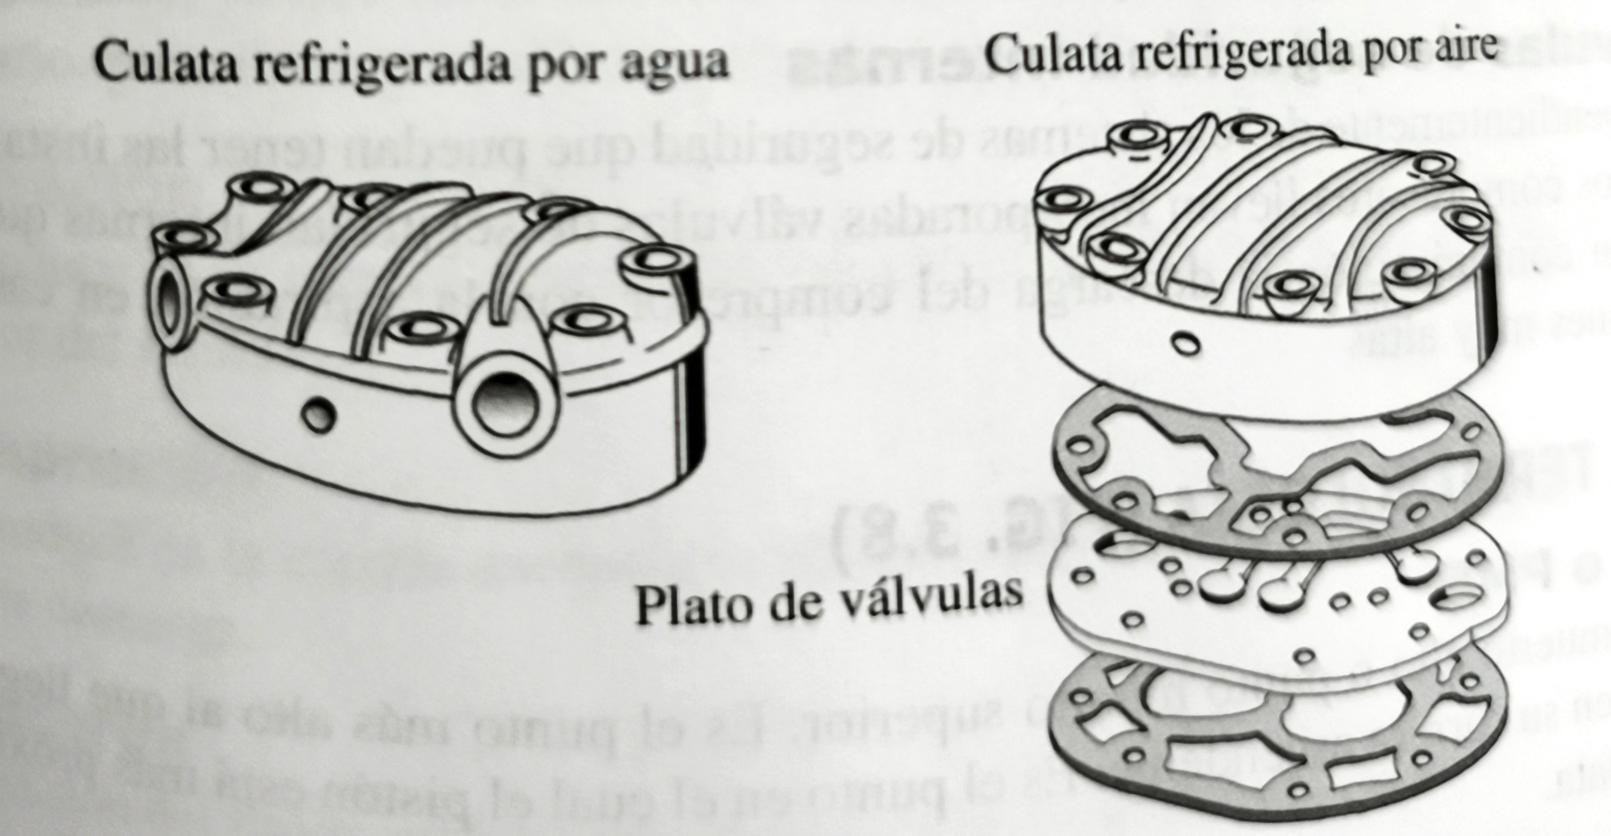
\includegraphics[width=.5\textwidth]{figuras/compresores/culata.jpg}
	\caption{Culatas refrigeradas por aire y por agua}
	\label{fig:Culatas refrigeradas por aire y por agua}
\end{figure}
\textbf{V\'alculas de aspiración y descarga}\\
Se encargan de comunicar el interior del cilindro con los conductos de aspiraci\'on y descarga. Su apertura y cierre se producen por la diferencia de presiones entre la del interior del cilindro y la de los conductos respectivos del fluido. Por lo general son de acero inoxidable, y para grandes potencias, dispotnen de resortes para su accionamiento.\\
\textbf{V\'alvulas de seguridad internas}\\
Independientemente de los sistemas de seguridad que puedan tener las instalaciones, los compresores llevan incorporadas v\'alvulas de seguridad internas que ponen en comunicaci\'on la descargas del compresor con la aspiración en caso de presiones muy altas.

%\subsubsection{Terminología}

%\textbf{PMA o PMS}\\
%Punto muerto alto o punto muerto superio. Es el punto m\'as alto al que llega el pist\'on en su carrera ascendente. Es el punto en el que \'el pist\'on est\'a m\'as cerca de la culata.\\
%\textbf{PMB o PMI}\\
%Punto muerto bajo o punto muerto inferior, es el punto m\'as bajo al que llega el pist\'on en su carrera.\\
%\textbf{Carrera}\\
%Distancia entre el PMS y el PMI. Corresponde a un \'angulo de giro de 180° del cig\"ue\~{n}al.
%
%\begin{figure}[H]
%	\centering
%	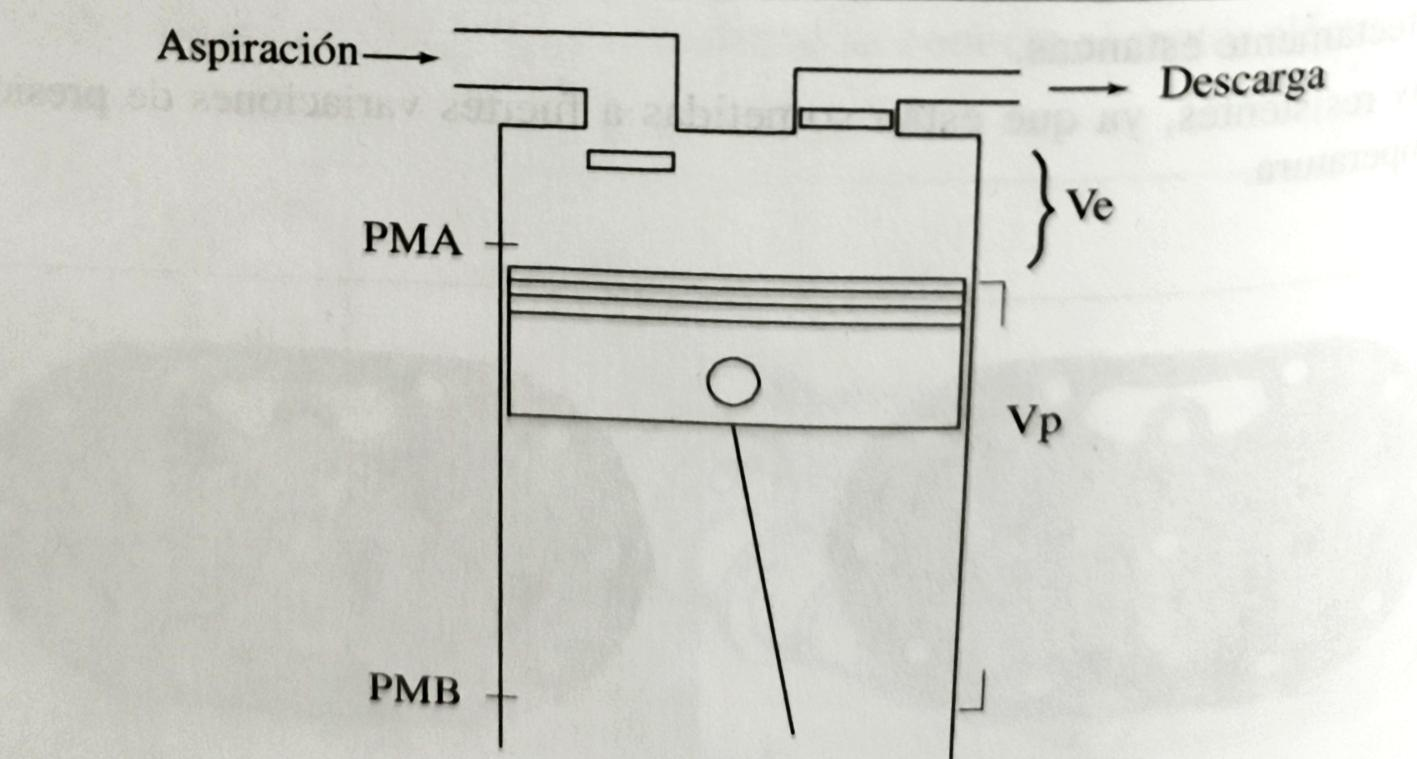
\includegraphics[width=.5\textwidth]{figuras/compresores/terminologia.jpg}
%	\caption{Terminolog\'ia de un cilindro en un compresor}
%	\label{fig:Terminolog\'ia}
%\end{figure}
%
%\textbf{Espacio neutro (Ve)}\\
%Es el comprendido entre el pist\'on cuando se encuentra en el PMS y la culata. Tambi\'en conocido como ``espacio muerto''.Tiene gran importancia en el rendimiento del compresor y est\'a determinado para evitar que el pist\'on, en su carrera ascendente, llegue a chocar con la culata, incluyendo las dilataciones que sufren los materiales, ya que est\'an sometidos a altas temperaturas. Debe ser el m\'inimo necesario, pues tiene gran repercusi\'on en el rendimiento volum\'etrico.\\
%\textbf{Aspiraci\'on}\\
%Se produce en la carrera descendente del pist\'on. Es la admisi\'on del fluido en el interior del cilindro.\\
%\textbf{Compresi\'on}\\
%Se produce en la carrera ascendente del pist\'on e inmediatamente despu\'es se realiza la descarga.\\
%\textbf{Descarga}\\
%Impulsi\'on del fluido refrigerante al conducto de descarga.\\
%\textbf{Volumen desplazado por el pist\'on (Vd)}\\
%El comprendido entre el PMS y PMI que desplaza el pist\'on en la carrera.\\
%\textbf{Volumen total del cilindro (Vt)}\\
%El comprendido entre el pist\'on cuando se encuentra en el PMI y la culata.
%\begin{equation*}
%	Vt = Ve + Vd
%\end{equation*}
%\textbf{Potencia indicada}\\
%Es la potencia que se genera en el interior del cilindro.\\
%\textbf{Potencia efectiva}\\
%Es la potencia que se debe suministrar con el motor el\'ectrico para que el compresor trabaje en las condiciones previstas. Es decir, es la potencia medida en el eje del compresor. Pero a partir de este punto se produce una disminuci\'on de la potencia ya que una parte de la misma se pierde en vencer los rozamientos de cojinetes, bielas, etc. Por ello, la potencia efectiva siempre ser\'a superior a la potencia indicada.
%\begin{equation*}
%	Pe > Pi
%\end{equation*}
%La potencia efectiva es la potencia de accionamiento.\\
%\textbf{Rendimiento mec\'anico}\\
%Es el valor que contempla las p\'erdidas de origen mec\'anico anteriormente mencionadas. Por lo tanto, es la relaci\'on entre ambas potencias:
%\begin{equation*}
%	\eta m = \frac{Pi}{Pe}
%\end{equation*}
\subsubsection{Funcionamiento}
Para facilitar su comprensi\'on vamos a ver como se producen los movimientos de apertura y cierre de las v\'alvulas de aspiraci\'on y descarga, con relaci\'on al movimiento del pist\'on.
\begin{enumerate}[a.]
	\item Carrera descendente:\\ Cuando el pistçón inicia la carrera descendente, hacia el PMI, crea en el interior del cilindro una depresi\'on que implica, que en su interior la presi\'on sea inferior a la existente en la parte superior de la v\'alvula, es decir en el conducto de aspiraci\'on, con lo que la v\'alvula de aspiraci\'on se abre (``baja'') y el fluido refrigerante entra en el cilindro.\\ El fluido entrar\'a en el cilindro hasta que se igualen las dos presiones, y en teor\'ia deber\'ia ser en cantidad igual a la correspondiente al volumen del cilindro, pero hay factores que impiden que entre esa cantidad.\\ La v\'alvula de descarga permanece cerrada, por la alta presi\'on existente en el conducto de descarga mientras el pist\'on se va acercando al PMI y la v\'alvula de aspiraci\'on contin\'ua abierta.\\ As\'i, cuando el pist\'on llega al PMI, la v\'alvula de aspiraci\'on est\'a abierta y la de descarga cerrada. El cig\"ue\~{n}al ha girado 180°.
	\item Carrera ascendente:\\ Cuando el pist\'on rebasa el PMI se inicia la carrera ascendente, y la v\'alvula de aspiraci\'on se cierra, porque la presi\'on en el interior del cilindro es superior a la existente en el conductor de aspiraci\'on. Con las dos v\'alvulas cerradas se inicia la compresi\'on del fluido (\autoref{fig:Carrera ascendente}A), y se produce:
	\begin{itemize}
		\item Una disminici\'on de volumen.
		\item Un aumento de la presi\'on y la temperatura, hasta que la primera alcanza un valor tal que hace que se abra (levante) la v\'alvula de descarga.
	\end{itemize}
	En la \autoref{fig:Carrera ascendente} se puede apreciar que poco antes de que el pist\'on llegue al PMS la v\'alvula de descarga abre (``hacia afuera''), porque la presi\'on en el interior del cilindro, en la carrera escendente, es superior a la del conducto de descarga y ``levanta'' la v\'alvula. El fluido es impulsado hacia el condensador.\\
	El cig\"ue\~{n}al ha girado 180°, con lo que las dos carreras consecutivas gir\'o 360°, es decir una vuelta.\\ Una vez rebasado el PMS, y con la v\'alvula de descarga cerrada, se reinicia el ciclo.
\end{enumerate}
\begin{figure}[H]
	\centering
	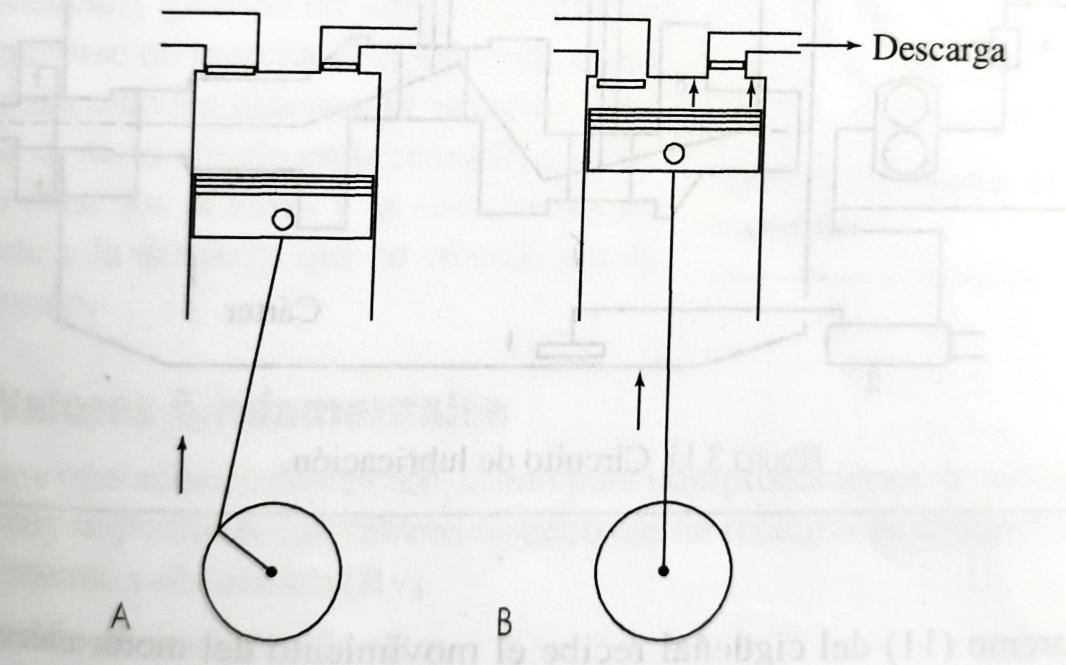
\includegraphics[width=.5\linewidth]{figuras/compresores/aspiracion y descarga.jpg}
	\caption{A = Compresi\'on. B = Descarga}
	\label{fig:Carrera ascendente}
\end{figure}
\subsubsection{Lubricación}
Es uno de los asprectos m\'as importantes del compresor y por lo tanto de la instalaci\'on. El tipo de lubricaci\'on empleada es forzada, mediante una bomba de engranajes que es accionada por el mismo motor el\'ectrico que acciona el compresor.\\ Anteriormente hemos comentado que a trav\'es de los aros de engrase, el aceite sale impulsado hacia las camisas. Pero tambi\'en se lubrican otras partes en movimiento como el cigueñal, cojinetes de bancada, cojinetes de biela y prensas principales.

Es importante saber que el circuito de aceite que conecta la bomba de engranajes con los dispositivos a lubricar cuenta con filtros y un enfriador de aceite, ya que este, adem\'as de lubricar, refrigera los elementos. El compresor tendr\'a enfriador de aceite dependiendo de su potencia, tipo y caracter\'isticas de funcionamiento.
\subsubsection{Valores fundamentales}
Tanto para operaciones de c\'alculo, como para comprobaciones de funcionamiento, son muy importantes los valores respectivos de relaci\'on de compresi\'on (Rc) y de rendimiento volum\'etrico (Rv).
\begin{enumerate}[1.]
	\item \textbf{Relaci\'on de compresi\'on (Rc)}
	\begin{equation*}
		Rc = \dfrac{\text{Presi\'on de descarga absoluta}}{\text{Presi\'on de aspiraci\'on absoluta}}
	\end{equation*}
	$\text{Presi\'on absoluta = Presi\'on manom\'etrica + Presi\'on atmosf\'erica}$
	\item \textbf{Rendimiento volum\'etrico (Rv)}\\ Se puede expresar de varias maneras, pero una de ellas a efectos pr\'acticos es:
	\begin{equation*}
		Rv = {\frac{\text{Volumen de vapor que realmente aspira}}{\text{Volumen te\'orico que tendr\'ia que aspirar}}X 100}
	\end{equation*}
	Cuanto mayor sea la relaci\'on de compresi\'on, menor ser\'a el rendimiento volum\'etrico y viceversa.

	Su valor depende de factores rales como el espacio neutro y la densidad del fluido en el interior del cilindro.
	\item \textbf{Volumen desplazado}\\ El volumen de fluido que en teor\'ia tiene que aspirar es el volumen desplazado por el pist\'on en su carrera. Como sabemos, el volumen de un cilindro es el producto del \'area por la altura:
	\begin{gather*}
		V = S \times h\\ 
		S = \pi\cdot r^2 = \pi\cdot(\frac{D}{2})^2 = \pi\cdot\frac{D^2}{4}
	\end{gather*}
	y la altura (h) es la distancia entre PMI y el PMS, o sea es la carrera:
	\begin{equation*}
		V = \frac{\pi D^2}{4}C
	\end{equation*}
	que es el volumen que desplaza el pist\'on en una revoluci\'on. Si gira el cig\"ue\~{n}al a n revoluciones por minuto y tiene N cilindros, el volumen desplazado ser\'a:
	\begin{equation*}
		Vd = \frac{\pi\cdot D^2\cdot C\cdot n\cdot N\cdot 60\cdot 10^-3}{4}(\frac{m^3}{h})
	\end{equation*}
\end{enumerate}
\subsection{Compresores herméticos}
Su \'ambito de aplicaci\'on comprende los sitemas de refrigeraci\'on y aire acondicionado.\\El motor el\'ectrico va acoplado directamente al compresor, y ambos dentro de la misma envolvente (carcasa) de acero formando una unidad. Al ser herm\'eticos (cerrados) no podemos acceder a ellos, como por ejemplo, para realizar operaciones de mantenimiento. Pueden ser alternativos, rotativos o de tornillo.\\ En su configuraci\'on (\autoref{fig:Compresor herm\'etico}), lleva tres tubos soldados a la carcasa. Dos son del mismo di\'ametro y el tercero menor. El de menor di\'ametro se conectar\'a a la descarga y la aspiraci\'on a cualquiera de los otros dos. Por lo general, se hace al tubo que est\'a al lado contrario de la placa de conexionado el\'ectrico, para evitr que las condensaciones que se puedan producir en el exterior del mismo, lleguen a introducirse a la placa.\\ De esta manera el otro tubo, que no se conecta la circuito, se puede utilizar para que, despu\'es de instalar una conexi\'on ob\'us o una v\'alvula de intervenci\'on, se aproveche para realizar operaciones tales como:
\begin{itemize}
	\item Meter carga de refrigerante
	\item Comprobar la presi\'on de aspiraci\'on
	\item Comprobar la temperatura de evaporaci\'on
	\item Meter aceite
\end{itemize}
\begin{figure}[H]
	\centering
	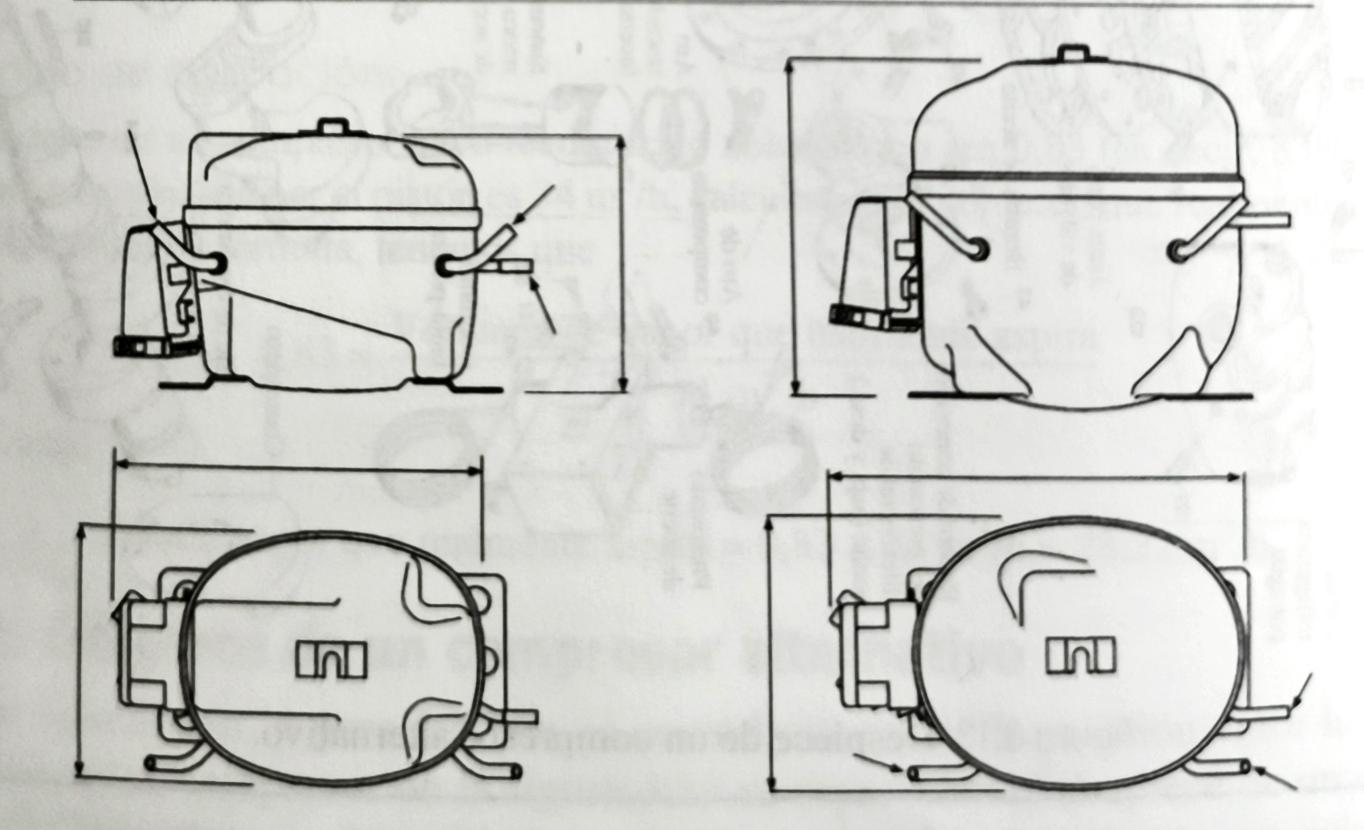
\includegraphics[width=.8\linewidth]{figuras/compresores/compresor herméticos.jpg}
	\caption{Compresor herm\'etico}
	\label{fig:Compresor herm\'etico}
\end{figure}
\subsubsection{Algunas caracter\'isticas}
\begin{enumerate}[1.]
	\item Son silenciosos porque cuentan con resortes interiores y c\'amaras silenciadoras que amortiguan el golpeteo de las v\'alvulas. Carecen de transmisiones exteriores como por ejemplo correas.
	\item Est\'an refrigeradores por el fluido de aspiraci\'on por lo que, la falta de fluido afectar\'ia a la refrigeraci\'on del compresor. Hay que evitar la humedad en el circuito y la entrada de l\'iquido al compresor porque estar\'ian en contacto con la parte el\'ectrica.
	\item Trabajar a temperaturas inferiores a las normales, implicar\'ia el aumento del volumen espec\'ifico, que afectar\'ia, entre otras cosas a la refrigeraci\'on.
\end{enumerate}
\subsection{Compresores semiherméticos}
Estos compresores en su funcionamiento tienen las mismas ventajas e inconvenientes que los herm\'eticos pero a diferencia que son m\'as accesibles para realizar mantenimiento. Por ejemplo, en compresores semiherm\'eticos alternativos se pueden desmontar para realizar operaciones de mantenimiento tales como cambiar pistones o aros.\\ Pueden ser enfriados externamente por aire o por agua.
\subsubsection{\'Acidos}
Es importante comentar que en los compresores, ya sean herm\'eticos o semiherm\'eticos, una de las aver\'ias m\'as importantes es la contaminaci\'on del circuito por \'acidos, puesto que se refrigeran por los vapores de aspiraci\'on. La presencia de \'acidos se produce por altas temperaturas en la zona que se encuentra entre el estator y rotor, esto genera que el fluido refrigerante reaccione y ataque los devanados del estator.\\ Las causas pueden ser varias pero se podr\'ia englobar en mantenimiento inadecuado, sobre carga del motor y elevadas temperaturas de trabajo.\\ Si se cambia un compresor por otro en un sistema contaminado por \'acidos y antes no se eliminan \'estos, atacar\'an a los aislamientos de los bobinados, con lo cual la duraci\'on del nuevo compresor ser\'a muy corta.
\subsection{Compresores abiertos}
Se llaman abiertos porque el motor el\'ectrico y el compresor est\'an separados. Por lo tanto, el fluido refrigerante ya no est\'a en contacto con la parte el\'ectrica, como ocurre en los compresores herm\'eticos y semiherm\'eticos. Como est\'an separados la conexi\'on entre ambos necesita de un sistema de estanqueidad o sello en ese punto para evitar las fugas del fluido refrigerante al exterior. El acoplamiento motor-compresor se puede realizar mediante correas, se puede adaptar la velocidad con sus di\'ametros (seg\'un necesidad de carga) o mediante dos platos met\'alicos unidos el\'asticamente.
\subsubsection{Caracter\'isticas de funcionamiento}
En estos compresores abiertos se considera buena relaci\'on de compresi\'on (Rc) si no excede de 10:1, ya que cuanto menor sea, mayor ser\'a el rendimiento volum\'etrico (Rv) y, por lo tanto, mayor ser\'a la potencia frogir\'ifica.\\ Si el compresor tuviera que trabajar con una Rc elevada, como sucede, por ejemplo, cuando se trata de instalaciones que necesiten temperaturas muy bajas para enfriar y las de condensaci\'on sean normales, entonces no se podr\'ia utilizar uno de simple etapa, porque entre otras cosas, las altas temperaturas afectar\'ian:
\begin{itemize}
	\item A los materiales (dilataciones)
	\item A la lubricaci\'on, perjudicar\'ia la viscosidad del aceite
	\item A las temperaturas de descarga, porque ser\'ian muy altas
	\item Y a los rendientos, que disminuir\'ian
\end{itemize}
Para solucionar estos inconvenientes tendr\'iamos que recurrir a los compresores de doble etapa (sistema compound), que tambi\'en se hace extensivo a los semiherm\'eticos.
\subsubsection{Compresores de doble etapa}
Los compresores de doble etapa reparten la elevada relaci\'on de presiones y disminuyen el alto recalentamiento. Cada secci\'on del compresor trabaja a menor presi\'on y tambi\'en menor temperatura de descarga, lo que implica un mejor aprovechamiento volum\'etrico. Para ello emplean un sistema de enfriamiento en la etapa intermedia, cuando es asi se los llama sistema por \textbf{inyecci\'on parcial}. Pero cuando se enfria el fluido en la etapa intermedia y, a su vez, antes de que \'este entre en el evaporador se lo llama sistema de \textbf{inyecci\'on total}.
\begin{itemize}
	\item \textbf{Inyecci\'on parcial:}\\ Se mezclan el fluido expansionado por la v\'alvula y los gases de descarga de los cilindros de baja en la tuber\'ia de presi\'on intermedia. De esta manera, se logra bajar la temperatura de descarga de los cilindros de alta.
	\item \textbf{Inyecci\'on total}\\ Se realiza un enfriamiento de los gases de descarga de los cilindros de baja y, a su vez, tambi\'en se hacen pasar el fluido expansionado por un intercambiador de calor para enfriar el refrigerante antes de entrar al evaporador e incrementar el efecto frigorífico.
\end{itemize} 
\subsection{Compresores rotativos}
Se caracterizan por comprimir el fluido refrigerante mediante el movimiento circular continuo de un rotor, que puede ser de exc\'entrica o de paletas.
\subsubsection{De exc\'entrica}
\begin{wrapfigure}{r}{0.45\linewidth}
	\centering
	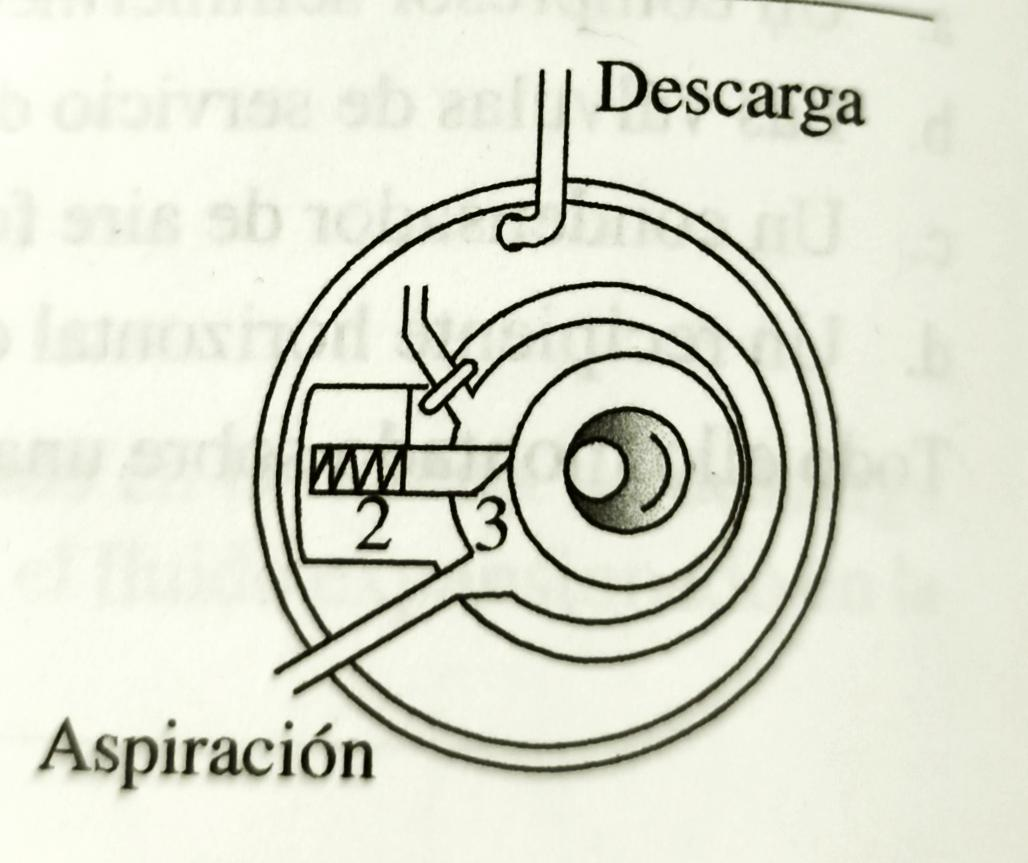
\includegraphics[width=.7\linewidth]{figuras/compresores/rotor de excentrica.jpg}
	\caption{Rotor de exc\'entrica}
	\label{fig:Rotor de exc\'entrica}
\end{wrapfigure}
Consta (\autoref{fig:Rotor de exc\'entrica}) de un rotor exc\'entrico respecto al cilindro donde se aloja y que en su movimiento llega a establecer contacto con \'el.\\Este rotor, por acci\'on del resorte (2) est\'a permanentemente en contacto con una paleta (3).\\Esta paleta, tal como se aprecia en la figura, establece la separaci\'on entre las c\'amaras de aspiraci\'on y de descarga. En su funcionamiento, la aspiraci\'on se realiza de manera continua, y al disminuir el espacio comprendido entre el rotor y el cilindro, se efect\'ua la comprensi\'on del fluido refrigerante y posterior descarga.

\subsubsection{De paletas}

B\'asicamente (\autoref{fig:Rotor de paletas}) consta de un rotor montado en el interior de un cilindro y cuyos centros ent\'an ligeramente desplazados. Este rotor aloja unas paletas que est\'an comprimidas contra la pared del cilindro por medio de unos resortes. Al pasar cada paleta por el orificio de la aspiraci\'on, se crea una depresi\'on que provoca la entrada del fluido en el espacio comprendido entre esa paleta y la anterior. Posteriormete y dado que el espacio entre el rotor y el cilindro disminuye, tambi\'en lo hace el volumen del fluido (compresi\'on) hasta que alcanza el orificio de descarga.\\ Existen compresores cuyos rotores no llevan resortes y las paletas se mantienen comprimidas por la acci\'on de su propio peso y de la fuerza centr\'ifuga.

\begin{figure}[H]
	\centering
	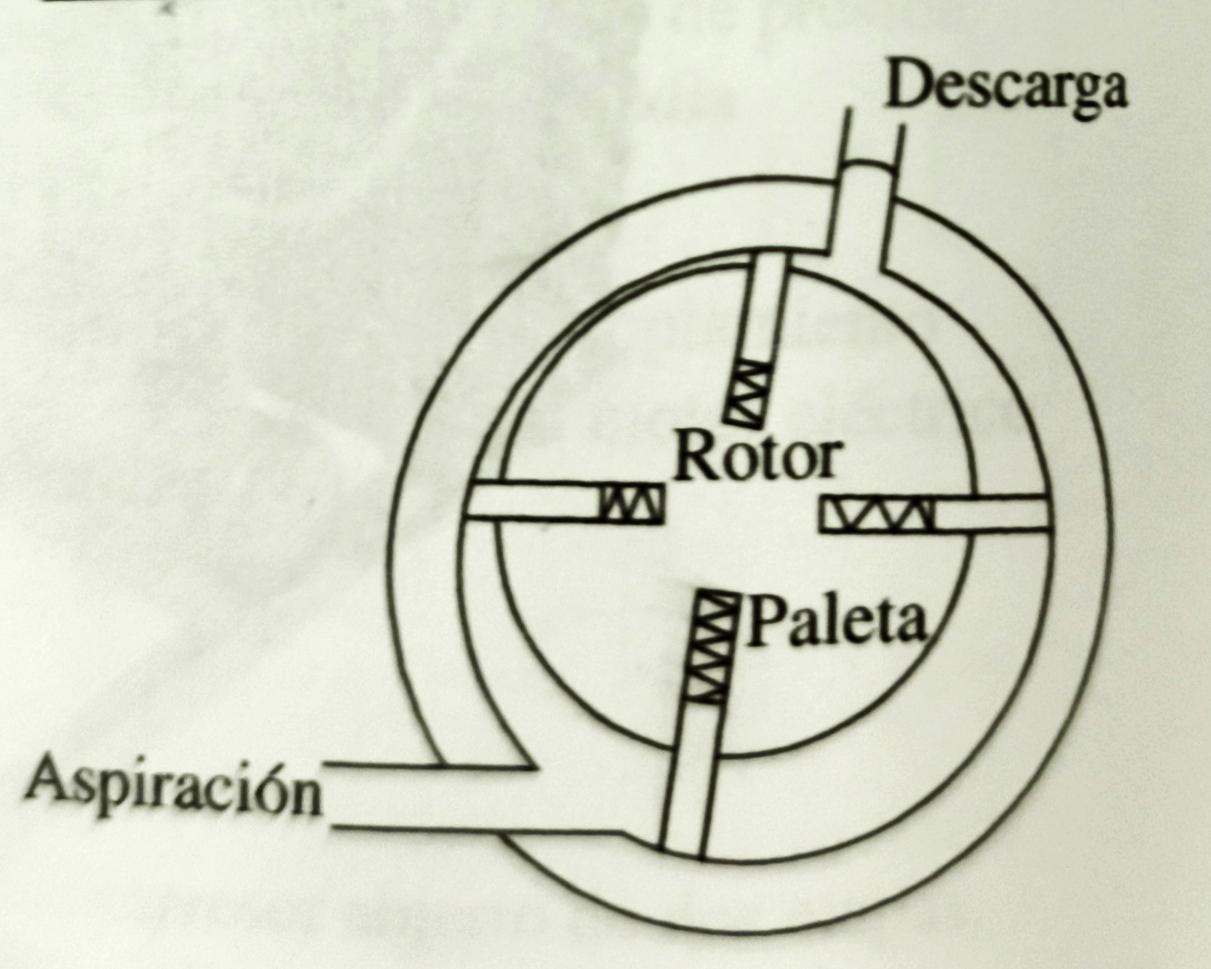
\includegraphics[width=.4\linewidth]{figuras/compresores/rotor de paletas.jpg}
	\caption{Rotor de paletas}
	\label{fig:Rotor de paletas}
\end{figure}

\subsection{Compresores helicoidales}

Los compresores helicoidales o de tornillo son distintos a los anteriormente vistos. La compresi\'on del fluido es continua. Constan de dos rotores llamados primario y secundario que, montados en ambos extremos sobre cojinetes, aseguran su exacta posici\'on en el interior del compresor. El \textbf{rotor primario}, de cuatro l\'obulos o helicoides, es accionado directamente por el motor el\'ectrico y gira a la misma velocidad que \'este.\\ Mediante un sistema de rodamientos, el rotor primario transmite el movimiento al \textbf{rotor secundario}, que tiene seis l\'obulos o helicoides y es del mismo di\'ametro, pero gira a menor velocidad y en sentido contrario.\\ Entre los dos rotores existe una separaci\'on muy pequeña, es decir, no est\'an en contacto entre s\'i.\\Al girar ambos rotores dentro de la cavidad del compresor y debido a esa pequeña separaci\'on, se producen las aberturas de espacios en la zona de aspiraci\'on que con el giro van disminuyendo, con lo que se translada y comprime el fluido hacia el otro extremo de los rotores, donde se produce la descarga del fluido refrigerante.\\ Los hay de tipo herm\'etico, semiherm\'etico y abiertos.
\subsubsection{Importancia del aceite}
Estos compresores helicoidales llevan unos grandes separadores de aceite. Este es inyectado a lo largo de los tornillos para su lubricaci\'on y sellado al mismo tiempo, lo que facilita la compresi\'on del fluido.\\ La \autoref{fig:Circuito de aceite en instalaciones con compresores a tornillo} representa una aplicaci\'on muy utilizada de estos compresores.\\Como consecuencia de la alta temperatura que alcanza el aceite, a la salida del separador y antes de volver al compresor, suele pasar por un enfriador, que seg\'un las caracter\'isticas de la instalaci\'on, puede utilizar aire, agua o el mismo refrigerante para el enfriamiento del aceite.\\ Los factores que determinan si es necesario el enfriamiento del aceite son las condiciones de trabajo:

\begin{itemize}
	\item Temperatura de condensaci\'on
	\item Temperatura de evaporaci\'on
	\item Temperatura de descarga
\end{itemize}

\begin{figure}[H]
	\centering
	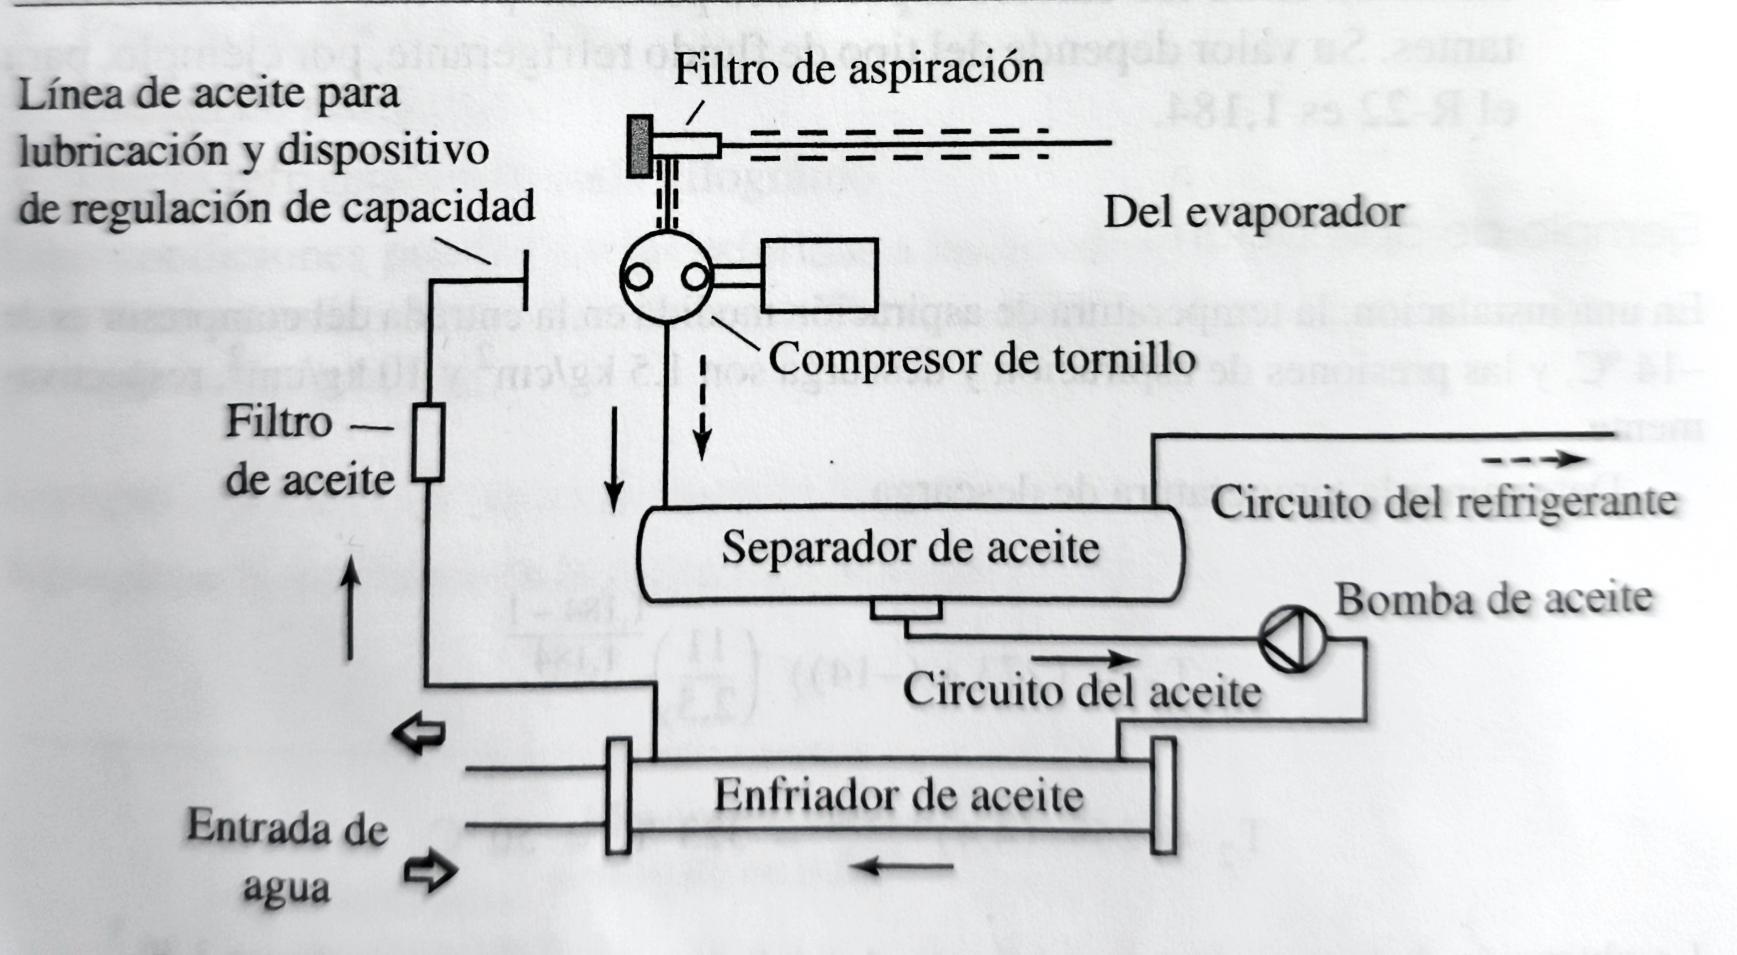
\includegraphics[width=\textwidth]{figuras/compresores/circuito de aceite (2).jpg}
	\caption{Circuito de aceite en instalaciones con compresor a tornillo}
	\label{fig:Circuito de aceite en instalaciones con compresores a tornillo}
\end{figure}

\subsection{Regulación de la potencia}

Si la carga de los evaporadoes siempre fuese la misma, se intalar\'ia el compresor a esa determinada carga t\'ermica. Pero como en la mayor\'ia de los casos la carga var\'ia (ejemplo m\'as notorio lo tenemos en las instalaciones de aire acondicionado), se debe encontrar un punto de equilibrio entre la carga producida por el compresor y la carga necesaria en el evaporador.\\Para los casos de pequeñas instalaciones, como pueden ser heladeras dom\'esticas, el compresor consume muy poca potencia. Por tanto estas instalciones generalmente trabajan con un sistema ON-OFF, donde consumen la potencia m\'axima y una vez que se llego al set point se apaga el compresor.\\En cambop en instalaciones de mayores potencias hay que conseguir un equilibrio entre la carga producida y la necesaria, lo cual significa menores consumos y menos mantenimiento.

\subsubsection{Sistema de regulaci\'on}

La regulaci\'on se puede realizar de varias maneras, por ejemplo actuando sobre el volumen desplazado o bien sobre las revoluciones del motor, ya que la potencia es directamente proporcional a las revoluciones.\\Acontinuaci\'on se presenta un sistema de regulaci\'on para compresores a tornillo:

\begin{enumerate}[a.]
	\item Instalando entre la parte inferior de los rotores y el fondo del c\'arter un dispositivo deslizante (pist\'on), que es accionado por la presi\'on del aceite (mediante electrov\'alvula), y que al desplazarse a lo largo de los rotores, su posici\'on marca el ``punto'' de inicio de la compresi\'on del fluido y determina as\'i el desplazamiento volum\'etrico del compresor.
	\item Mediante controles deslizantes (pistones) instalados en el extremo final de la brida de descarga.
\end{enumerate}

La \autoref{fig:Disposici\'on de los controles de capacidad} representa un compresor semiherm\'etico, en vista superior. La entrada de fluido refrigerante es a trav\'es de la v\'alvula de aspiraci\'on situada en el lado izquierdo, y la descarga (oculta) est\'a en el lado derecho.\\La regulaci\'on de la potencia se realiza mediante las dos electrov\'alvulas y los dos pistones montados en el extremos de la brida de descarga (m\'etodo b.)

\begin{figure}[H]
	\centering
	\includegraphics[width=\textwidth]{figuras/compresores/controles de capacidad.jpg}
	\caption{Disposici\'on de los controles de capacidad}
	\label{fig:Disposici\'on de los controles de capacidad}
\end{figure}

\begin{wrapfigure}{r}{0.5\linewidth}
	\centering
	\includegraphics[width=.7\linewidth]{figuras/compresores/detalle de control de capacidad.jpg}
	\caption{Detalle de control de capacidad}
	\label{fig:Detalle de control de capacidad}
\end{wrapfigure}

Los dos pistones son accionados hidr\'aulicamente. Mediante una señal el\'ectrica se abren unos orificios debidamente calibrados, y as\'i una parte del fluido es conducido hacia el lado de la aspiraci\'on (en la \autoref{fig:Detalle de control de capacidad} se aprecia en detalle la operaci\'on)\\Al disminuir el caudal de fluido descargado, tambi\'en se disminuye la potencia. En este sistema, la regulaci\'on de potencia se realiza en dos etapas. Cuando una electrov\'alvula no \'esta activada, se produce una reducci\'on de potencia.

\subsection{Variaciones de las presiones y su repercursión en las potencias}

La potencia frigor\'ifica de un compresor dependen de las condiciones de trabajo. Por ello vamos a ver de que manera repercuten en la potencia frigor\'ifica las variaciones de las presiones de trabajo.\\ En el diagrama de Mollier podemos apreciar c\'omo var\'ia la potencia frigor\'ifica seg\'un las distintas temperaturas de evaporaci\'on y condensaci\'on.
% \renewcommand{\theenumi}{\alph{enumi}}
\begin{enumerate}[a.]
	\item ¿Qu\'e ocurre cuando la presi\'on de aspiraci\'on disminuye?\\ Supongamos que la presi\'on de aspiraci\'on $Pa$, disminuye hasta un valor $Pa^\prime$\\Se comprueba que:
	\begin{enumerate}[1.]
		\item Al disminuir la presi\'on de aspiraci\'on, el efecto refrigerante ($ER^\prime$) tambi\'en disminuye con lo cual disminuye la potencia.
		\item El volumen espec\'ifico ($Ve^\prime$) aumenta, lo que implica que el desplazamiento volum\'etrico disminuye.
	\end{enumerate}

	\begin{figure}[H]
		\centering
		\includegraphics[width=.6\textwidth]{figuras/compresores/variacion de la presion de aspiracion.jpg}
		\caption{Variaci\'on de la psei\'on de aspiraci\'on en el diagrama p-h.}
		\label{Variaci\'on de la presi\'on de aspiraci\'on}
	\end{figure}
	Tambi\'en se puede demostrar num\'ericamente con la relaci\'on de compresi\'on (Rc) para este caso aumenta, por tanto disminuye el rendimiento volum\'etrico (Rv) y la potencia frigor\'ifica.

	\item ¿Qu\'e ocurre con la potencia frigor\'ifica cuando disminuye la presi\'on de condensaci\'on?\\Viendo la \autoref{fig:Variaci\'on de la presi\'on de condensaci\'on} se puede ver que:
	\begin{enumerate}[1.]
		\item El efecto refrigerante ($ER^\prime$) aumenta, con lo que la potencia frigor\'ifica tambi\'en aumenta.
		\item La relaci\'on de compresi\'on (Rc) disminuye, con lo que la potencia frigor\'ifica aumenta.
	\end{enumerate}
	\begin{figure}[H]
		\centering
		\includegraphics[width=.6\textwidth]{figuras/compresores/variacion de la presion de condensacion.jpg}
		\caption{Variaci\'on de la presi\'on de condensaci\'on en el diagrama p-h}
		\label{fig:Variaci\'on de la presi\'on de condensaci\'on}
	\end{figure}
\end{enumerate}
La \autoref{fig:Capacidad de un compresor modelo 4RD} es un ejemplo es informaci\'on t\'ecnica de un compresor modelo 4RD, en ella podemos corroborar lo anteriormente dicho:
\begin{enumerate}[a.]
	\item Si la temperatura de condensaci\'on es 30\textcelsius\ y de evaporaci\'on -5\textcelsius, entonces su capacidad ser\'a de 11800 kcal/h.
	\item En cambio, si la temperatura de condensaci\'on es de 50\textcelsius\ y la de evaporaci\'on es de -5\textcelsius, entonces su capacidad se reduce a 9400 kcal/h.
\end{enumerate}
\begin{figure}[h]
	\centering
	\includegraphics[width=\linewidth]{figuras/compresores/tabla de capacidad de un compresor.jpg}
	\caption{Capacidad de un compresor modelo 4RD}
	\label{fig:Capacidad de un compresor modelo 4RD}
\end{figure}
\subsection{Funcionamiento en régimen seco y en régimen húmedo}
Se dice que trabaja en \textsl{r\'egimen h\'umedo} cuando el fluido a la entrada del compresor es una mezcla de gas y l\'iquido (Tramo 1-2 de la \autoref{fig:R\'egimen seco y h\'umedo}). Esto puede ocurrir por diversas causas, tales como:
\begin{enumerate}[a.]
	\item Mala regulaci\'on del dispositivo de expansi\'on y entra demasiado fluido refrigerante en el evaporador.
	\item Mala circulaci\'on del aire a trav\'es del evaporador por obstrucci\'on o por caudal insuficiente.
\end{enumerate}
Pero en esa mezcla, la cantidad de l\'iquido a\'un no es lo suficiente importante para producir el golpe de l\'iquido, ya que se va evaporando debido a las temperaturas m\'as altas que se va encontrando, por ejemplo:
\begin{enumerate}[a.]
	\item En la conexi\'on tuber\'ia de aspiraci\'on-compresor
	\item En la culata
	\item En el pist\'on
	\item En la camisa
	\item Durante la fase de compresi\'on 
\end{enumerate}

\begin{wrapfigure}{r}{0.5\linewidth}
	\centering
	\includegraphics[width=.8\linewidth]{figuras/compresores/régimen seco y humedo.jpg}
	\caption{R\'egimen seco y h\'umedo}
	\label{fig:R\'egimen seco y h\'umedo}
\end{wrapfigure}

Pero ese calor que absorbe el l\'iquido lo est\'a haciendo del calor proveniente del compresor e instalaci\'on y no del ambiente a refrigerar (en el evaporador).\\ En cambio, cuando el fluido a la entrada del compresor es vapor (Tramo 3-4 de la \autoref{fig:R\'egimen seco y h\'umedo}), entonces se trata del \textbf{r\'egimen seco} y, en este caso, el rendimiento es mayor que en el caso anterior. Pero se debe tener especial cuidado para este tipo de funcionamiento, ya que si el vapor que entra al compresor est\'a demasiado sobrecalentado puede generar temperaturas de descarga elevadas por lo que el rendimiento del ciclo ser\'a perjudicado (Tramo 5-6 de la \autoref{fig:R\'egimen seco y h\'umedo}).		
		
\section{Aver\'ias y soluciones}

En este apartado se nombran algunas de las aver\'ias m\'as comunes que pueden suceder en los sistemas de refrigeraci\'on.

\subsection{Aumento excesivo de la presi\'on de descarga}

\begin{table}[H]
    \begin{center}
        \begin{tabular}{p{10cm} p{5cm}}
            \textbf{Causa} & \textbf{Remedio} \\ \hline
            Poco caudal de agente condensante o que la temperatura de entrada del mismo es muy alta & Regular\\
            Condensador sucio & Limpiar\\
            Gases incondensables en el circuito & Purgar\\
            Sobrecarga de refrigerante & Sacar refrigerante\\
            Condensador de poca capacidad & Sustituir\\
            Bomba de circulaci\'on de agua defectuosa & Comprobar y/o reparar\\
            Ventilador del condensador defectuoso & Comprobar y/o reparar\\
            Man\'ometro defectuoso & Reparar o renovar\\
            Separador de aceite no trabaja bien & Revisar\\ \hline
        \end{tabular}
    \end{center}
\end{table}

\subsection{Presi\'on de descarga muy baja}

\begin{table}[H]
    \begin{center}
        \begin{tabular}{p{8cm} p{7cm}}
            \textbf{Causa} & \textbf{Remedio}\\ \hline
            Man\'ometro defectuoso & Comprobar y/o cambiar\\
            Cantidad de fluido refrigerante escasa & Reparar fugas, en caso de que las haya, y recargar\\
            Condensador demasiado grande & Comprobar con datos de c\'alculo\\
            Caudal de agua o aire, a trav\'es del condensador, excesivo & Ajustar\\
            Temperatura de agua o aire, a trav\'es del condensador demasiado baja & Ajustar caudal\\
            Caudal de aire o temperatura excesivos a trav\'es del condensador & Comprobar variadores de velocidad o automatismos (por ejemplo, presostatos) que act\'uan sobre los ventiladores\\
            V\'alvulas de descarga del compresor defectuosas & Comprobar, reparar y/o cambiar\\
            V\'alvulas de aspiraci\'on parcialmente cerrada & Abrir la v\'alvula\\
            Aros de pist\'on muy desgastados & Comprobar y sustituir\\ \hline
        \end{tabular}
    \end{center}
\end{table}

\subsection{Presi\'on de aspiraci\'on muy alta}

\begin{table}[H]
    \begin{center}
        \begin{tabular}{p{8cm} p{7cm}}
            \textbf{Causa} & \textbf{Remedio}\\ \hline
            Man\'ometro defectuosos & Comprobar\\
            V\'alvula o v\'alvulas de aspiraci\'on del compresor defectuosas & Comprobar, reparar y/o cambiar\\
            V\'alvula de expansi\'on termost\'atica demasiado abierta & Comprobar y/o ajustar\\
            Capacidad del compresor muy pequeña & Comprobar con datos de c\'alculo y caracter\'isticas de funcionamiento. Comprobar regulador de capacidad.\\
            V\'alvula interna de seguridad del compresor que no est\'a totalmente cerrada & Comprobar y ajustar\\
            Demasiada carga t\'ermica & Reducir carga\\ \hline
        \end{tabular}
    \end{center}
\end{table}

\subsection{Presi\'on de aspiraci\'on muy alta}

\begin{table}[H]
    \begin{center}
        \begin{tabular}{p{8cm} p{7cm}}
            \textbf{Causa} & \textbf{Remedio}\\ \hline
            Man\'ometro defectuoso & Comprobar\\
            Capacidad de la v\'alvula de expansi\'on insuficiente & Comprobar con datos de c\'alculo\\
            V\'alvula de expansi\'on obstruida & Limpiar\\
            V\'alvula de expansi\'on con igualador externo de presi\'on & Comprobar si el igualador externo est\'a montado y si es as\'i, si es el adecuado\\
            El bulbo de la v\'alvula de expansi\'on est\'a montado en un punto demasiado fr\'io & Cambiar y comprobar\\
            La instalaci\'on tiene poca carga de fluido refrigerante & Meter carga con previa comprobaci\'on de fugas\\
            Filtros (de l\'inea de l\'iquido y/o de l\'inea de aspiraci\'on) sucios & Limpiar\\
            V\'alvula/s manual/es en l\'inea de aspiraci\'on parcialmente cerrada/s & Comprobar y abrir\\
            V\'alvula solenoide cerrada total o parcialmente & Comprobar suciedad o bobina\\ \hline
        \end{tabular}
    \end{center}
\end{table}

\subsection{Presi\'on de aceite muy alta}

\begin{table}[H]
    \begin{center}
        \begin{tabular}{p{8cm} p{7cm}}
            \textbf{Causa} & \textbf{Remedio}\\ \hline
            Man\'ometro defectuoso & Comprobar\\
            Filtro de la bomba de aceite sucio & Limpiar o sustituir\\
            Presostato diferencial de aceite no est\'a debidamente ajustado & Comprobar y ajustar\\ \hline
        \end{tabular}
    \end{center}
\end{table}

\subsection{Presi\'on de aceite muy baja}

\begin{table}[H]
    \begin{center}
        \begin{tabular}{p{8cm} p{7cm}}
            \textbf{Causa} & \textbf{Remedio}\\ \hline
            Man\'ometro defectuoso & Comprobar\\
            Filtro de aspiraci\'on de la bomba de aceite sucio & Limpiar o cambiar\\
            Presencia de fluido refrigerante en estado l\'iquido en el c\'arter & Comprobar separador\\
            Bajo nivel de aceite en el c\'arter & Cargra hasta nivel normal de aceite\\
            Demasiada holgura en los cojinetes del compresor & Comprobar, reparar y/o cambiar los cojinetes\\
            Presostatos diferencial de aceite no est\'a ajustado correctamente & Comprobar y ajustar\\ \hline
        \end{tabular}
    \end{center}
\end{table}

\subsection{El compresor carga y descarga intermitentemente}

\begin{table}[H]
    \begin{center}
        \begin{tabular}{p{8cm} p{7cm}}
            \textbf{Causa} & \textbf{Remedio}\\ \hline
            V\'alvula de expansi\'on demasiado grande, que ocasiona una gran fluctuaci\'on en la presi\'on de aspiraci\'on & Comprobar capacidad de la v\'alvula\\
            Control de presi\'on de aceite defectuoso & Verificar nivel de aceite y/o v\'alvula de seguridad de la bomba de aceite\\ \hline
        \end{tabular}
    \end{center}
\end{table}
		\chapter{Evaporadores}
\section{Generalidades}


	El evaporador es el componente del sistema de refrigeración utilizado para absorber el calor del ambiente y transferirlo al refrigerante que circula por su interior. Está compuesto por tubos, pasajes o recipientes hechos generalmente de cobre o aluminio para diámetros pequeños y de cobre y acero para diámetros grandes.
	
	
	
%	Absorbe el calor debido al refrigerante contenido en los tubos. Contiene, además, un fluido (o producto refrigerante) que está separado del refrigerante por las paredes o carcasa del intercambiador.
	
	\section{Clasificación}
	\subsection{Clasificación según su construcción}
	
		Existen tres tipos generales de evaporadores
		\begin{itemize}
			\item de tubos desnudos,
			\item de superficie extendida,
			\item y de placas.
		\end{itemize}
	
		\subsubsection{Evaporadores de tubos desnudos}
		
			Están formados por tubos (generalmente de cobre o acero) sin aletas ni elementos que aumenten la superficie de transferencia de calor.
			\begin{figure}[h]
				\centering
				\begin{subfigure}{.4\linewidth}
					\includegraphics[width=\linewidth]{evaporadores/evaporador-tubo-1}
					
				\end{subfigure}
			\begin{subfigure}{.4\linewidth}
				\includegraphics[width=\linewidth]{evaporadores/evaporador-tubo-2}
				
			\end{subfigure}
			\caption{Evaporadores de tubo.}
			\label{fig:evaporadores-tubo}
			\end{figure}
			
			Los tubos de acero se utilizan en evaporadores grandes y en evaporadores que utilicen amoníaco como refrigerante, mientras que los tubos de cobre se emplean en evaporadores pequeños y se los usa con refrigerante que no sea amoníaco.
			
			Estos evaporadores se forman en una amplia variedad de tamaños, forma y diseños, y es muy común que sean fabricados a la medida según el diseño.
	
		\subsubsection{Evaporadores de superficie extendida}
		
			Están formados por un serpentín de tubería en la que se aplican aletas de aluminio para aumentar la superficie de transmisión del propio tubo.
			
			\begin{figure}[h]
				\centering
				\begin{subfigure}{.4\linewidth}
					\includegraphics[width=\linewidth]{evaporadores/evaporador-superficie-1}
				\end{subfigure}
			\begin{subfigure}{.4\linewidth}
				\includegraphics[width=\linewidth]{evaporadores/evaporador-superficie-2}
			\end{subfigure}
			\caption{Evaporadores de superficie extendida.}
			\label{fig:evaporadores-superficie}
			\end{figure}
			
			Cuando se agregan aletas al serpetín, éstas se extienden hacia afuera y actúan como colectores de calor. Aboserben calor del aire que ordinariamente no estaría en contacto con la superficie de los tubos desnudos, y conducen este calor hacia la tubería.
			
			
			Para que las aletas sean eficientes deberán estar unidas a la tubería de manera tal que se asegure un buen contacto térmico. En algunos casos las aletas están soldadas directamente a los tubos, mientras que en otros casos, las aletas se hacen deslizar sobre la tubería y se expande a esta última, por lo que permite una correcta sujeción.
		
		
			El tamaño del tubo determina el tamaño de la aleta, y el espaciamiento entre cada una de ellas varía según el tipo de aplicación. Para aplicaciones a muy bajas temperaturas, se produce un inevitable acumulamiento de escarcha entre las aletas, lo que tiende a restringir el paso de aire a través del serpentín. Es por ese motivo que para este tipo de aplicaciones, los evaporadores deberán tener un mayor espaciamiento (dos o tres aletas por pulgada) a fin de minimizar daños por la restricción en la circulación del aire. Mientras que, para aplicaciones donde los serpentines trabajan a temperaturas suficientemente altas, de tal modo que no se produzca escarcha sobre la superficie, podrán tenerse hasta 14 aletas por pulgada. No obstante, un aleteado excesivo podrá reducir la capacidad del evaporador porque restringiría innecesariamente la circulación de aire a través del serpentín.
		
			
			
		
		\subsubsection{Evaporadores de placas}
		
		
			Consisten en la unión de dos placas unidas herméticamente con un circuito trazado en su interior por donde circulará el refrigerante.
			
			La superficie plana de las placas pueden ser fabricadas en una diversidad de formas y los pasajes de refrigerantes pueden ser integrales o adheridos. Algunos son construidos con dos placas planas de metal realzadas y soldadas una con otra de tal modo que pueda fluir el refrigerante entre ambas, mientras que en otros se tiene una tubería instalada entre dos placas metálicas las cuales están soldadas por sus orillas.			
			
			\begin{figure}[h]
				\centering
				\begin{subfigure}{.4\linewidth}
				\includegraphics[width=\linewidth]{evaporadores/evaporador-placa-1}
				\end{subfigure}
				\begin{subfigure}{.4\linewidth}
				\includegraphics[width=\linewidth]{evaporadores/evaporador-placa-2}
				\end{subfigure}
				\caption{Evaporadores de placa.}
				\label{fig:evaporadores-placa}
			\end{figure}
	
	\subsection{Clasificación según la circulación del aire}	
	
	La circulación de aire en un espacio refrigerado es esencial para la transferencia de calor del producto hacia el evaporador. En productos que no están envasados a prueba de vapor, la inadecuada circulación puede ser determinante. Cuando la circulación de aire es muy grande, se aumenta la rapidez de evaporación de la humedad lo que produce una deshidratación en el producto. Mientras que, una escasa circulación de aire favorece el crecimiento de hongos y bacterias. Por otra parte, cuando el producto está envasado a prueba de vapor no se verá afectado por altas velocidades y la velocidad de circulación de aire se debe mantener en un nivel alto para obtener un efecto de enfriamiento máximo.
	
	La circulación de aire deseada varía con las diferentes aplicaciones y depende sobre todo de la humedad del espacio, del tipo de producto y del período de tiempo de almacenaje. 
	
	Los evaporadores se pueden clasificar según la circulación de aire sobre el serpentín en evaporadores de \emph{convección natural} y de \emph{convección forzada}.
	
	\subsubsection{Evaporadores de convección natural}
	
	Se usan frecuentemente en aplicaciones donde se desea aire de baja velocidad y deshidratación mínima del producto. Son instalaciones típicas las que se tienen en unidades de exhibición, enfriadores con pasillo interior y en cuartos grandes de almacenaje. En la \autoref{fig:conveccion-natural} se muestra un evaporador de este tipo.
	
	
	\begin{figure}[h]
		\centering
		\includegraphics[width=.5\linewidth]{evaporadores/natural}
		\caption{Evaporador de techo de convección natural.}\label{fig:conveccion-natural}
	\end{figure}
	
	La circulación de aire sobre el serpentín se da por el diferencial de temperatura y densidad del aire entre el evaporador y el espacio. A mayor diferencia de temperatura, mayor será la velocidad de circulación del aire. Esta depende de la forma, tamaño y localización del evaporador, por el uso de desviadores y por la colocación del producto en el espacio.
	
	A causa de que el movimiento de aire es por el fenómeno de convección natural, el consumo en este tipo de instalaciones es menor respecto al de convección forzada.
	
	\subsubsection{Evaporadores de convección forzada}
	
	Conocidos comercialmente por el nombre de \emph{unidad enfriadora}, se caracterizan por estar equipados con ventiladores para forzar la circulación de aire sobre el serpentín. La \autoref{fig:conveccion-forzada} muestra un ejemplo de evaporador con dos ventiladores.
	
	\begin{figure}[h]
		\centering
		\includegraphics[width=.5\linewidth]{evaporadores/forzados}
		\caption{Evaporador de convección forzada.}\label{fig:conveccion-forzada}
	\end{figure}
	
	\subsection{Clasificación según el método de alimentación del refrigerante}
		
		Los evaporadores también pueden ser clasificados de acuerdo al método de alimentación del líquido refrigerante como evaporadores de \emph{expansión seca}, \emph{inundados} y \emph{sobrealimentados}.
		
		
			\subsubsection{Evaporador de expansión seca}
				
				Como se observa en la \autoref{fig:expansion-directa}, en el evaporador de expansión seca la mezcla de gas y líquido refrigerante que sale de la válvula de expansión entra directamente al serpentín. Parte de la masa, la que se encuentra en fase líquida, se vaporiza progresivamente a medida que el refrigerante pasa a través del evaporador.
			
			
				Los evaporadores de expansión seca son menos eficientes que los de otro tipo, pero son por lo general mucho más simples en su diseño, más económicos, requieren menos carga de refrigerante y tienen menos problemas que los demás en lo que respecta al regreso del aceite. Por estas razones, los evaporadores de expansión seca son el tipo más popular.
				
				
				\begin{figure}[h]
					\centering
					\includegraphics[width=.7\linewidth]{evaporadores/expansion-directa}
					\caption{Evaporador de expansión seca.}
					\label{fig:expansion-directa}
				\end{figure}
		
		
			\subsubsection{Evaporador inundado}
			
				Los evaporadores inundados se llenan completamente con el refrigerante líquido a fin de tener humedecida toda la superficie interna del tubo, y en consecuencia, la mayor razón posible de transferencia de calor.
				
				Como se muestra en la \autoref{fig:inundado}, el evaporador está equipado con un acumulador o colector de vapor que sirve como receptor de líquido, desde el cual solo el refrigerante líquido es circulado por gravedad a través del serpentín. 
				
				El vapor generado por la ebullición del refrigerante en los tubos del evaporador y el vapor flash, se separan del líquido en la parte superior del acumulador de donde es sacado directamente a través de la línea de succión para continuar su ciclo hacia el compresor.
				
				
				\begin{figure}[h]
					\centering
					\includegraphics[width=.7\linewidth]{evaporadores/inundado}
					\caption{Evaporador inundado.}
					\label{fig:inundado}
				\end{figure}
		
			\subsubsection{Evaporador sobrealimentado}
			
				Los evaporadores sobrealimentados son un tipo especial del sistema de evaporador inundado, también se denominan como evaporadores recirculados o de circulación forzada. Cuentan con una bomba para forzar la circulación del refrigerante a través del serpentín. Son más comunmente empleados en sistemas de evaporador múltiple, como se ve en la \autoref{fig:sobrealimentado}.
		
				\begin{figure}[h]
					\centering
					\includegraphics[width=.9\linewidth]{evaporadores/sobrealimentado}
					\caption{Evaporador de líquido sobrealimentado.}
					\label{fig:sobrealimentado}
				\end{figure}
				
				En este tipo de sistema se minimizan los problemas relacionados con el retorno de aceite en el evaporador. Además, a diferencia del sistema inundado en el que líquido refrigerante circula por acción de la gravedad, el sistema sobrealimentado presenta la ventaja de que el tanque acumulador no requiere estar ubicado necesariamente por encima del evaporador.
		
	\subsection{Clasificación según la transmisión del frío}
	
			Los sistemas se pueden clasificar según la forma en la que el espacio es refrigerado en sistemas \emph{directos} e \emph{indirectos}.
			
			\subsubsection{Sistemas directos}
				
			Un sistema de refrigeración por expansión directa, también llamado de refrigeración directa, es aquel en el que el refrigerante circula por el evaporador y entra en contacto directo con el medio o el espacio que se desea enfriar, sin utilizar un fluido intermedio. Este tipo de sistema es común en heladeras, aires acondicionados y cámaras frigoríficas pequeñas por su eficiencia y simplicidad.
				
			\subsubsection{Sistemas indirectos}
				
				Los sistemas de refrigeración indirecta emplean agua o salmuera empleadas como \emph{refrigerante secundario} para refrigerar el espacio. El refrigerante primario enfría al secundario y luego este se dirige para entrar en contacto directo con el espacio o producto a refrigerar.
				
				Estos sistemas se emplean cuando el lugar a refrigerar está a una distancia considerable del equipo de condensación. El uso del sistema indirecto evita problemas como el retorno de aceite y las excesivas caídas de presión en las tuberías. Además, las fugas causan problemas serios y es más fácil de que ocurran en tuberías con refrigerante que en tuberías con agua o salmuera. Por otra parte, son empleados con ventaja en instalaciones donde la fuga del refrigerante y/o aceite pueda contaminar al producto, como en plantas empacadoras de carne o en grandes aplicaciones de almacenes fríos en los cuales se usa amoníaco como refrigerante primario.
				
				Algunos refrigerantes secundarios son agua, cloruro de calcio y salmueras como cloruro de sodio, flicoles de etileno y propileno, y metanol.
		
	\section{Capacidad del evaporador}\label{sec:capacidad-evaporador}
	
		El calor puede llegar al evaporador por los tres métodos de transferencia de calor conocidos. De todas maneras, éste debe pasar por \emph{conducción} al refrigerante en el interior a través de las paredes del evaporador. La cantidad de calor transferido por conducción a través de cualquier superficie se expresa como
		
		\begin{equation}\label{eq:calor}
			Q = A \cdot U \cdot D
		\end{equation}
		
		Donde \begin{itemize}
			\item $Q$ es la cantidad de calor transferido por hora,
			\item $A$ es el área de la superficie exterior del evaporador,
			\item $U$ es el coeficidente total de transferencia,
			\item $D$ es la diferencia de temperatura media logarítmica entre la temperatura del evaporador y la temperatura del refrigerante.
		\end{itemize}
	
	
			\subsection{Coeficiente total de transferencia}
				
				La resistencia al flujo de calor ofrecida por las paredes del evaporador es suma de tres factores, cuya relación queda expresada como
				
				\begin{equation}\label{eq:conductancia-total}
					\dfrac{1}{U} = \dfrac{R}{f_i} + \dfrac{L}{k} + \dfrac{1}{f_o}
				\end{equation}
				
				donde \begin{itemize}
					\item $U$ es el coeficiente total de transferencia,
					\item $L/k$ es la resistencia al flujo de calor ofrecida por el metal de los tubos y aletas,
					\item $R$ es la relación de superficie exterior a superficie interior,
					\item $f_i$ es el factor de conductancia de la película de la superficie interior,
					\item $f_o$ es el factor de conductancia de la película de la superficie exterior.
				\end{itemize}
				
				El coeficiente total de transferencia deberá ser lo más grande posible para tener una alta transferencia de calor a través de las paredes del evaporador. Generalmente, se emplean metales para la construcción de los evaporadores. Sin embargo, debe tenerse en consideración el tipo de refrigerante que se emplee para evitar reacciones no deseadas con el metal. 
		
				
				Los metales que se usan con mayor frecuencia, son: hierro vaciado, acero, cobre, latón y aluminio. El hierro vaciado y el acero no se ven afectados por ninguno de los refrigerantes más comunes, no obstante, se oxidan al haber humedad en el sistema. El latón y el cobre pueden usarse con cualquier refrigerante menos con el amoníaco, el cual disuelve el cobre. El aluminio puede utilizarse con cualquier refrigerante menos con el cloruro de metilo.\\
				
				De los tres términos involucrados en la \autoref{eq:conductancia-total}, aquellos que involucran los coeficientes de conductancia de las superficies de película son los mayores y, por tanto, de mayor interés.
				
				
				En relación con esto, la transferencia de calor por conducción es mayor a través de líquidos que a través de gases, y la rapidez a la cual el refrigerante transfiere calor incrementa a medida que lo hace la superficie humedecida. En este aspecto, los evaporadores inundados, dado que están completamente llenos de líquido, son más eficientes que los del tipo expansión seca. Este principio también se aplica a la superficie externa del evaporador.
		
		
				Cualquier suciedad que se tenga ya sea en las superficies externas o internas, tienden a actuar como aislamiento térmico y a diminuir el factor de conductancia. El aislamiento externo o suciedad en la superficie externa del evaporador puede deberse a
				
				\begin{itemize}
					\item la suciedad originada por polvos que lleva el aire y se adhieren a la superficie,
					\item la formación de incrustaciones y a la oxidación,
					\item la formación y acumulación de escarcha.
				\end{itemize}
				
				La suciedad en la superficie interna de los tubos del evaporador se puede originar por
				
				\begin{itemize}
					\item cantidades excesivas de aceite en el evaporador,
					\item bajas velocidades del refrigerante, generando acumulación de burbujas debido a la acción de ebullición del fluido.
				\end{itemize}
				
				En relación con la velocidad del fluido, la conductancia de la película en la superficie puede mejorarse al aumentar la velocidad del fluido. Sin embargo, en el interior de los tubos, la velocidad está limitada por la máxima caída de presión admisible a través del serpentín. Mientras que, la velocidad del fluido sobre la superficie externa del serpentín está limitada por otras consecuencias que no son en sí mismo la capacidad del evaporador.
				
				
				\emph{Cualquier incremento que se tenga en la turbulencia del flujo, ya sea dentro o fuera del evaporador, aumentará considerablemente la tasa de transferencia de calor a través de las paredes del evaporador}. 
				
				En general, la tuberbulencia interna se aumenta con la diferencia de temperatura a través de las paredes del tubo. La turbulencia externa está influida por la velocidad del fluido sobre el serpentín, por el espaciamiento de los tubos y por la forma de las aletas.\\
				
			\subsection{Ventajas de usar aletas}
				
				La ventaja del aleteado depende de los coeficientes de conductancia de las superficies de película exterior e interior, y de la relación $R$ entre dichos valores. 
				
				
				% Acá habla de la tasa de transferencia de calor en las superficies. Tengo entendido que esto funciona como un cuello de botella: se espera que ambas superficies, externa e interna, tengan la misma tasa. Sin embargo, en instalaciones de aire, la superficie interna tiene una tasa mayor por lo que se aumenta la superficie externa con aleteados para incrementar la externa. Mientras que, en instalaciones donde el serpentín está en contacto con líquido se utilizan tubos desnudos.
				En instalaciones de refrigeración de aire la rapidez de flujo de calor en la superficie exterior es menor que la de superficie interior, por lo que la capacidad total del evaporador estará limitada por la capacidad de la superficie exterior. Para estos casos, el valor total de $U$ puede incrementarse usando aletas para aumentar el área de la superficie exterior hasta un valor tal que la cantidad de calor absorbido por la superficie exterior sea aproximadamente igual a la que pueda pasar por la superficie interior. Por otra parte, en aplicaciones donde el líquido esté en contacto en ambos lados del tubo y en los que la transferencia de calor es aproximadamente igual para ambas superficies, los evaporadores de tubo descubierto muestran una alta eficiencia y el aleteado no es necesario.	\\
		
				En algunas instalaciones con enfriamiento de líquido que utilizan refrigerantes fluorocarburos, la rapidez de transferencia de calor sobre el lado del fluido enfriado puede exceder a la rapidez sobre el lado del refrigerante, en cuyo caso el aleteado del tubo en el lado del refrigerante mejorará el rendimiento del evaporador. En la \autoref{fig:aleteado-interno} se muestran varios ejemplos de aleteado interno.
			
				\begin{figure}[h]
					\centering
					% Columna izquierda - subfigura (a)
					\begin{subfigure}{0.58\linewidth}
						\centering
						\includegraphics[width=\linewidth]{evaporadores/aleteado-interno-1}
					\end{subfigure}
					% Columna derecha con subfigura (b) y (c)
					\begin{subfigure}{0.3\linewidth}
						\centering
						\includegraphics[width=\linewidth]{evaporadores/aleteado-interno-2}
						
						\vspace{0.3cm}
						
						\includegraphics[width=.7\linewidth]{evaporadores/aleteado-interno-3}
					\end{subfigure}
					
					\caption{Algunos ejemplos de aleteado interno.}
					\label{fig:aleteado-interno}
				\end{figure}
			
			\subsection{Diferencia de temperatura media logarítmica}
			
				La diferencia de temperatura media real del aire, también conocida como temperatura efectiva media (METD), se obtiene como el promedio logarítmico entre las temperaturas de entrada y salida del aire. Se calcula según la \autoref{eq:metd}, asumiendo que la temperatura del refrigerante ($T_r$) se mantiene constante durante el proceso.
				
				\begin{equation}\label{eq:metd}
					D = \dfrac{(T-e - T_r) - (T_s - T_r)}{\ln\dfrac{T_e - T_r}{T_s - T_r}}
				\end{equation}
				Donde\begin{itemize}
					\item $D$ es la diferencia de temperatura efectiva media,
					\item $T_e$ es la temperatura del aire que llega al serpentín,
					\item $T_s$ es la temperatura del aire a la salida del serpentín,
					\item $T_r$ es la temperatura del refrigerante en los tubos.
				\end{itemize}
				
%				La \autoref{fig:curva-d} muestra el punto medio (METD) de la curva que representa la disminución de la temperatura a través del serpentín. Nótese que la disminución no es lineal, debido al hecho de que es mayor la diferencia de temperatura entre el aire y el refrigerante en la primera hilera, volviéndose menor y menor a medida que atraviesa el evaporador.
%				
%				\ver{agregar imagen jaja}
		
			\subsection{Área superficial}
				
				%Acá habla de la superficie, el número de hileras y la velocidad del aire sobre el serpentín.
				
				Según la \autoref{eq:calor}, la capacidad del evaporador aumenta o disminuye en proporción directa al cambio del área, sin embargo, esto es cierto para aquellos casos en los que no varíen los factores $U$ y $D$. Para muchos casos, dichos valores no son constantes y se ven afectados cuando cambia el área superficial del evaporador.
				
				
				Para ilustrarlo, en la \autoref{fig:disposicion-serpentines} se muestran tres disposiciones de serpentines. Los serpentines B y C tienen el doble del área superficial del serpentín A. No obstante, el aumento de capacidad con respecto a la capacidad del serpentín A, será mayor para el serpentín C que para el serpentín B.
				
				
				\begin{figure}[H]\centering
%					\begin{subfigure}{.3\linewidth}
%						\includegraphics[width=\linewidth]{evaporadores/serpentin-a}
%					\end{subfigure}	
%					\begin{subfigure}{.3\linewidth}
%						\includegraphics[width=\linewidth]{evaporadores/serpentin-b}
%					\end{subfigure}	
%					\begin{subfigure}{.3\linewidth}
%						\includegraphics[width=\linewidth]{evaporadores/serpentin-c}
%					\end{subfigure}

					\includegraphics[width=.7\linewidth]{evaporadores/disposicion-serpentin}
					\caption{Los serpentines B y C tienen el doble de área superficial que el serpentín A. El serpentín C tiene doble área en el frente que el serpentín A o B.}
					\label{fig:disposicion-serpentines}
				\end{figure}
				
				En un serpentín de varias hileras, a medida que el aire pasa a través de estas, en cada hilera subsiguiente se tendrá una menor razón de transferencia de calor y funcionará con menos eficiencia que la hilera anterior. La METD es afectada cuando el área superficial del serpentín es aumentada al aumentar el número de hileras (profundidad). Suministrando aire a la misma velocidad, la METD a través de C será exactamente igual a la que se tiene a través de A, y por lo tanto la capacidad de C será el doble que la del serpentín A.
				
				\emph{Para la misma área superficial total, un serpentín largo, ancho y plano, será más eficiente que otro serpentín corto y angosto que tenga más profundidad}.
				
				Sin embargo, en muchas aplicaciones, el espacio físico es limitado, debiendo usarse arreglos con serpentines compactos. En algunas ocasiones, la pérdida de capacidad resultante por el incremento de la profundidad es compensada aumentando la velocidad del aire sobre el serpentín.
				
				Además, en algunas aplicaciones, es deseable tener serpentines profundos para propósitos de deshumidificación. Cuando el aire húmedo pasa por un serpentín cuya superficie tiene una temperatura por debajo del punto de rocío del aire, el vapor de agua condensa en forma de gotas. Al tener más hileras de tubos, el aire permanece más tiempo en contacto y su temperatura se aproximará más a la temperatura de la superficie del serpentín.
			
				
			\subsection{Circuitos en el evaporador}
			
			
			Los evaporadores de múltiples circuitos se utilizan cuando en el serpentín se produce una caída de presión demasiado grande para un solo circuito.
			
			Una caída de presión excesiva en el evaporador da como resultado una presión menor que la realmente necesaria en la succión de vapor a la entrada del compresor. Debido a esto, un buen diseño requiere de varios circuitos en el evaporador, de modo que la caída de presión sea la mínima necesaria para tener velocidades suficientes en el refrigerante, favoreciendo así una tasa alta de transferencia de calor al eliminar las burbujas de aire en la superficie del tubo y asegurando un buen retorno del aceite (aspectos tratados en la \autoref{sec:capacidad-evaporador}).
			
			En general, la caída de presión en el evaporador dependerá del tamaño del tubo, de la longitud y de la carga en el circuito. La carga\footnote{Por carga en el circuito se entiende la rapidez de flujo de calor a través de las paredes del tubo.} determina la cantidad de refrigerante que debe pasar a través del circuito. A mayor carga, mayor deberá ser la cantidad del refrigerante que fluya a través del circuito y mayor será la caída de presión.
			
			Se diseñan varias disposiciones de circuitos. En la bibliografía \cite[Sección 11.12]{dossat2004refrigeracion} se mencionan los siguientes circuitos:
			\begin{itemize}
				\item \textbf{Circuito serie simple.} El refrigerante sigue un solo camino a través de todo el evaporador. Los evaporadores con esta disposición, según la \autoref{fig:circuito-1}, trabajarán en forma satisfactoria dentro de ciertos límites de carga, ya que, cuando se exceda dicho límite la velocidad alcanzará valores no deseados provocando una gran caída de presión.
				\begin{figure}[h]
					\centering
%					\includegraphics[width=.5\linewidth]{circuito-1}
					\caption{Evaporador con un circuito refrigerante en serie.}
					\label{fig:circuito-1}
				\end{figure}
				
				\item \textbf{Circuito dividido.} A causa de la caída de presión al final de la disposición anterior se divide al circuito en dos trayectorias. Esto produce el efecto de reducir la velocidad del refrigerante a la mitad del valor y la caída de presión hasta la octava parte. Esto permitirá tener una mayor carga en el serpentín sin excederse de los límites. Como ejemplo, se muestra la \autoref{fig:circuito-2}.
				\begin{figure}[h]
					\centering
%					\includegraphics[width=.5\linewidth]{circuito-2}
					\caption{Evaporador con un circuito refrigerante dividido.}
					\label{fig:circuito-2}
				\end{figure}
				\item \textbf{Circuitos múltiples paralelos}. Se instalan cabezales en los extremos del evaporador para permitir que el refrigerante sea distribuido de manera simultánea a través de varios circuitos paralelos. Existen diferentes configuraciones posibles, dependiendo de la orientación de los circuitos y del sentido del flujo entre el aire exterior y el refrigerante. Es importante tener en cuenta la orientación, ya que influye directamente en la distribución de la carga, pudiendo provocar un reparto no uniforme del refrigerante entre los circuitos. Esto ocurre, por ejemplo, en la \autoref{fig:circuito-3}, donde la temperatura del aire que atraviesa el serpentín es mayor en los primeros circuitos y va disminuyendo a medida que se incrementa la profundidad, y en consecuencia, requieren de más refrigerante. En cambio, las \autoref{fig:circuito-4} y \autoref{fig:circuito-5} muestran una configuración donde solucionan este inconveniente.
				\begin{figure}[h]
					\centering
					\begin{subfigure}{.3\linewidth}
%						\includegraphics[width=.5\linewidth]{circuito-3}
						\caption{Evaporador de cuatro circuitos con cabezales de refrigerante. Con flujo cruzado de aire y refrigerante da como resultado una carga desigual.}
						\label{fig:circuito-3}
					\end{subfigure}
					\begin{subfigure}{.3\linewidth}
%						\includegraphics[width=.5\linewidth]{circuito-4}
						\caption{Evaporador con distribuidor de refrigerante y cabezal. Arreglo en contraflujo.}
						\label{fig:circuito-4}
					\end{subfigure}
					\begin{subfigure}{.3\linewidth}
%						\includegraphics[width=.5\linewidth]{circuito-5}
					\end{subfigure}
					\caption{Evaporador de cinco circuitos con cabezales de refrigerante. Arreglo en contraflujo y menor profundidad, permitiendo un diferencial de temperatura media mayor.}
					\label{fig:circuito-5}
				\end{figure}
			\end{itemize}
			
			% Acá se menciona al circuito simple, luego, una mejora de este es un circuito con refrigerante dividido (el circuito se divide en el punto que la velocidad alcanza la máxima permitida y luego se divide en dos trayectorias paralelas) Esto reduce la velocidad a la mitad y la caída de presión se reduce hasta la octava.
			% Evaporador de varios circuitos con cabezal a la entrada y salida. La desventaja es el desequilibrio de carga que hay en cada circuito, ya que la diferencia de temperatura es mayor en la primera hilera en contacto con la corriente de aire y se va reduciendo a mayor profundidad, y requiere mayor carga. Es imposible ajustar con una alimentacion simple de refrigerante para satisfacer a cada circuito sin subalimentar o sobrealimentar a los otros. Este tipo es más utilizado en sistemas inundados.
			% Mejora del anterior con sistema a contraflujo.
			% Evaporador con distribuidor a la entrada y salida (cabezales, supongo) pero el refrigerante circula en contraflujo con el aire. La transferencia de calor es mayor para este caso y la carga en los circuitos es regular. 
			
	
	\section{Sistemas de desescarche}
		
		La escarcha se forma en el evaporador debido al congelamiento de la humedad presente en el aire que lo atraviesa. Si bien el amplio espaciamiento entre las aletas permite inicialmente el paso del flujo de aire aun con algo de escarcha acumulada, con el tiempo esta se incrementa hasta bloquear el paso del aire. Además, la escarcha actúa como un aislante térmico, disminuyendo la eficiencia en la transferencia de calor. 
		
		Por esta razón, el serpentín requiere un proceso de descongelado, deshielo o desescarche periódico, que asegure un flujo de aire adecuado y una refrigeración eficiente.
		
		La acumulación de escarcha depende de las condiciones y la temperatura de evaporación del aire.
		
		Los métodos de descongelación pueden ser clasificados, según la fuente de calor utilizada, como
			\begin{itemize}
				\item \emph{desescarche natural},  utiliza el calor del aire que se tiene en el espacio refrigerado,
				\item \emph{desescarche con calor suplementario}, se obtiene con el calor suministrado de otras fuentes que no sean el calor del espacio refrigerado, como agua, salmuera, resistencias eléctricas y gas caliente.
			\end{itemize}
			
			Todos los métodos de desescarche natural requieren que el sistema (o el evaporador) esté detenido por un período de tiempo suficiente largo que le permita al evaporador elevar la temperatura hasta un nivel superior al punto de congelamiento.
			
			Independientemente del sistema que se utilice, excepto en el desescarche por aire, para realizar la descongelación hay que desconectar el ventilador del evaporador durante el proceso de descongelación, u ocurrirán dos cosas:
			\begin{itemize}
				\item El calor de la descongelación se transferirá directamente al espacio acondicionado.
				\item El aire acondicionado frío ralentizará el proceso de descongelación.
			\end{itemize}
			
			En general, las etapas para el proceso de deshielo son:
			\begin{itemize}
				\item Corte del suministro de refrigerante al evaporador. Se cierra la válvula que se tiene en la tubería del líquido.
			%	Orden de inicio de desescarche; puede ser manual o automática. Comienza cuando se detiene la inyección de refrigerante líquido en el interior del evaporador.
				\item Evaporación del refrigerante en el interior del evaporador. Este proceso se puede realizar continuando con la producción frigorífica si el compresor continúa funcionando debido a un retardo programado. Mientras que en otros sistemas se detienen el compresor y los ventiladores.
			%Evaporación del líquido del interior del evaporador; este proceso se puede realizar continuando con la producción frigorífica si programamos un retardo y mantenemos funcionando el compresor para mantener la presión baja en el evaporador y los ventiladores para favorecer el intercambio de calor. Sin embargo en otros sistemas, se detiene el compresor y los ventiladores con lo que se aumenta la duración del desescarche y la energía necesaria para este, pues habrá que suministrar energía no sólo para producir la fusión del hielo sino que también habrá que suministrar energía para producir la evaporación del refrigerante que queda en el interior del evaporador tras cesar la inyección.
			
			%Retardo 1; en algunos sistemas de desescarche, como los de gas caliente, será necesario efectuar un retardo para realizar ajustes en los sistemas que intervienen en el proceso (seguridad en la apertura y cierre de las válvulas).
				\item Este proceso puede realizarse con los ventiladores en funcionamiento, como en el caso del desescarche por aire, o, como es más habitual, deteniendo su funcionamiento para evitar la dispersión del calor.
			%Fusión del hielo; se trata de aportar energía para elevar la temperatura y lograr la fusión del hielo acumulado. Este proceso se puede realizar con los ventiladores funcionando, como en los desescarches por aire, o como es habitual, parando los ventiladores; esto dependerá de las características de la cámara o mueble frigorífico. En los sistemas modernos en los que el tiempo se define por la sonda final de desescarche, se suele programar una duración máxima de desescarche y si no se alcanzara la temperatura deseada en el tiempo fijado, se lanzará una alarma al sistema. Esto puede producirse por una avería en el sistema de desescarche (resistencias) o por no haber detenido la inyección de líquido. También se puede producir esta anomalía por haber mantenido la puerta de la cámara abierta durante largos periodos de tiempo o por alguna rotura en los cerramientos que provoque infiltraciones de aire exterior.
			
			%Retardo 2; en este punto, algunos sistemas necesitan efectuar un retardo para realizar ajustes en los sistemas que intervienen en el desescarche (islas de congelados).
				\item Drenaje del evaporador. Es necesario establecer un tiempo adicional para facilitar la evacuación de los condensados generados tras la fusión del hielo.
			%Tiempo de goteo o drenaje del evaporador; es necesario dar un tiempo para facilitar la evacuación de los condensados producidos tras la fusión del hielo debido a la apertura de las válvulas de aspiración en desescarche por gas caliente.
				\item Inyección de refrigerante. En esta etapa se reintroduce el refrigerante en el evaporador. Si queda agua remanente tras el desescarche, esta puede volver a congelarse al restablecerse las condiciones de funcionamiento.
			%Inyección de refrigerante; se vuelve a introducir refrigerante en el evaporador, y comienza a congelarse el agua que pueda quedar mojando las aletas y los tubos.
				\item Retardo en el funcionamiento de los ventiladores. Es importante llevar a cabo este paso una vez iniciada la inyección de líquido, para evitar que el agua presente sobre las aletas sea arrastrada y proyectada hacia el espacio refrigerado.
			%Retardo de conexión de los ventiladores; es importante retardar la conexión de los ventiladores tras comenzar la inyección de líquido para evitar que el agua que pueda estar mojando las aletas sea proyectada hacia la cámara. Este retraso permite que esta agua se congele. La conexión de los ventiladores se producirá al sobrepasar el tiempo indicado en el temporizador o bien cuando se detecte una temperatura por debajo del punto de congelación en la sonda final de desescarche. El retraso de conexión de los ventiladores también puede ser consecuencia de que en grandes evaporadores de cámaras de temperaturas muy bajas, se produce la conexión de los ventiladores estando el evaporador muy caliente, se puede predecir una onda expansiva por choque térmico al ponerse en contacto aire frio de la cámara y aire caliente del evaporador.
			\end{itemize}
			
		\subsection{Descongelamiento por aire}
		
		El método utiliza el calor del aire que se tiene en el espacio refrigerado para fundir el hielo del evaporador. Consiste en apagar el sistema de refrigeración y permitir que el aire no refrigerado circule sobre el serpentín. Dado que el aire se encuentra a una temperatura superior a la de la escarcha, facilita su derretimiento. Este tipo de descongelamiento por aire puede ser más lento que otros métodos y su eficacia dependerá tanto de la temperatura del aire como de la cantidad de escarcha acumulada.
		
		Este método resulta útil y es utilizado para temperaturas del evaporador superiores a 1°C.
		
		\subsection{Descongelamiento por agua}
		
		En el método de desescarche por agua se rocía agua sobre el serpentín del evaporador para derretir la escarcha. Generalmente, se sigue el siguiente procedimiento:
		\begin{enumerate}
			\item Se cierra la válvula del suministro de refrigerante y es evacuado del evaporador.
			\item Se detiene el compresor y los ventiladores para que el agua atomizada no ingrese al espacio refrigerado.
			\item Inicia el funcionamiento de los atomizadores de agua hasta que el evaporador sea deshielado, lo cual, según \cite{dossat2004refrigeracion}, requiere aproximadamente 4 a 5 minutos.
		\end{enumerate}
		
		Cuando se utiliza salmuera o una solución anticongelante, la solución no se desperdicia sino que regresa a un depósito para después hacerla circular.	
		
		Para evaporadores cuya temperatura baja hasta aproximadamente $-40$ °C, el deshielo se efectúa rociando agua sobre la superficie de los serpentines del evaporador. Para evaporadores cuya temperatura sea inferior a $-40$ °C, podrá sustituirse el agua por salmuera o alguna solución anticongelante.
		
		\subsection{Descongelamiento eléctrico}
		
		La descongelación eléctrica se realiza utilizando calentadores eléctricos situados en el evaporador. El compresor se detiene y estos calentadores se activan para realizar la descongelación, permitiéndoseles trabajar hasta que haya derretido todo el hielo del serpentín.
		
		\begin{figure}[h]
			\centering
%			\includegraphics[width=.5\linewidth]{descarche-electrico}
		\end{figure}
		
		\subsection{Descongelamiento por gas caliente}
		
		El descongelamiento por gas caliente tiene muchas variaciones, pero esencialmente, en este método se utiliza como fuente el calor interno del sistema proveniente del gas descargado por el compresor. 
		
		
		Se instala una válvula solenoide en un tubo de desviación instalado entre la descarga del compresor y la entrada del evaporador. Cuando la válvula está abierta, el gas expandido circula desde el compresor hacia el evaporador cediendo su calor al evaporador frío y se condensada. Parte del refrigerante condensado permanece en el evaporador, mientras que el resto regresa al compresor donde es evaporado por el calor de la compresión y recirculado al evaporador. 
		
		
		Una limitante de este método es que a medida que se da el descongelamiento, más líquido permanece en el evaporador y menos retorna al compresor, con el resultado de que el sistema agote su calor antes que el evaporador esté completamente deshielado. Otra desventaja es la posibilidad de que una capa pesada de refrigerante líquido regrese al compresor y cause daño en este.
		
		Estos inconvenientes se puede resolver proporcionando algunos medios para evaporar el refrigerante que condensa en el evaporador y los medios empleados distinguen a un método de otro.
		
		\subsection{Descongelamiento por inversión de ciclo}
		
		Se basa en el principio del ciclo invertido (bomba de calor), en donde el condensador puede utilizarse como serpentín para evaporar al refrigerante que se condensada en el evaporador durante el ciclo de desescarche. Para este tipo de operación se utilizan válvulas de 4 vías (\autoref{fig:valvula-4-vias}).
		
		La \autoref{fig:deshielo-bomba-calor} se muestra un esquema de flujo para las operaciones normal y de descongelamiento, respectivamente.
%		
%		\begin{figure}[h]
%			\begin{subfigure}{.4\linewidth}
%				\includegraphics[width=\linewidth]{inversion-1}
%				\caption{Operación normal}
%				\label{fig:inversion-1}
%			\end{subfigure}
%			
%			\begin{subfigure}{.4\linewidth}
%				\includegraphics[width=\linewidth]{inversion-2}
%				\caption{Operación de descongelamiento}
%				\label{fig:inversion-2}
%			\end{subfigure}
%			\caption{Esquema de flujo para un sistema de descongelamiento por ciclo invertido.}
%			\label{fig:deshielo-bomba-calor}
%		\end{figure} 
		
		
		\begin{figure}[h]
			\begin{subfigure}{.35\linewidth}
				\includegraphics[width=\linewidth]{evaporadores/inversion-3}
				\caption{Operación normal}
				\label{fig:inversion-3}
			\end{subfigure}
			
			\begin{subfigure}{.35\linewidth}
				\includegraphics[width=\linewidth]{evaporadores/inversion-4}
				\caption{Operación de descongelamiento}
				\label{fig:inversion-4}
			\end{subfigure}
			\caption{Esquema de flujo para un sistema de descongelamiento por ciclo invertido empleando una válvula de cuatro vías.}
			\label{fig:deshielo-bomba-calor}
		\end{figure} 
		\begin{figure}[h]
			\centering\caption{Válvula de cuatro vías.}
			\includegraphics[width=.5\linewidth]{evaporadores/images}
			\label{fig:valvula-4-vias}
		\end{figure}
		
	\section{Diseño y selección de evaporadores}
		
		Uno de los principales parámetros para el diseño de un evaporador es su capacidad de enfriamiento, vista en la \autoref{sec:capacidad-evaporador}. Otro de los factores más importantes a considerar en cualquier aplicación para la selección del evaporador adecuado es la \acrlong{dt}, ya que depende del tipo de aplicación y se determina en función de las condiciones de temperatura y humedad requeridas en el espacio.
		
		
		La selección del evaporador se realiza consultando los catálogos de los fabricantes. Debido a que calcular todas las variables que afectan su rendimiento no resulta práctico, generalmente, se determina a partir de ensayos reales. Aunque el método puede variar según el tipo de evaporador y el fabricante, las diferencias no suelen ser significativas y cada catálogo incluye instrucciones para interpretar correctamente los datos.
		
		\subsection{Dt del evaporador}
		
		El salto térmico del evaporador ($Dt$) es la diferencia de temperaturas entre la del fluido refrigerante, evaporándose en el interior del evaporador, y la del fluido a enfriar. 
		\begin{equation}
			Dt = t_c - t_e
		\end{equation}
		Donde 
		\begin{itemize}
			\item $t_e$ corresponde a la temperatura en el evaporador, o temperatura de evaporación,
			\item $t_c$ es la temperatura de la cámara o de diseño.
		\end{itemize}
		
		La Dt está condicionada por el tipo de aplicación debido a que tiene una gran influencia sobre la humedad relativa de la cámara, que a su vez está determinada por el tipo de producto\footnote{Cada producto tiene su propia temperatura y humedad relativa para poder ser mantenidos en óptimas condiciones de conservación o congelación.} en su interior. A partir del tipo de aplicación, se define la Dt del evaporador, lo cual permite establecer la temperatura de funcionamiento del mismo.
		
		El modelo de evaporador se debe elegir a partir de las tablas que figuran en los catálogos de los fabricantes, ya que es aquí donde aparecen todos los parámetros y factores de corrección que permiten indicar cuál es el más adecuado. Cada fabricante cuenta con sus propias tablas de selección y suelen ser diferentes entre un fabricante y otro.
		
		\subsection{Relación entre la Dt y la humedad relativa}
		
		La conservación de alimento y otros productos en condiciones óptimas de refrigeración, depende no únicamente de la temperatura del espacio refrigerado sino también de la humedad relativa en dicho espacio. Cuando es muy baja la humedad, se tiene una deshidratación excesiva. En caso contrario, cuando la humedad relativa es muy elevada, favorece el crecimiento de bacterias, hongos y se propicia una formación de una delgada capa de lama sobre el producto, y este último se da sobre todo en carnes.
		
		El factor más importante que regula la humedad es la $Dt$ del evaporador. Mientras menor sea esta diferencia de termperatura, mayor será la humedad relativa en el espacio refrigerado. Así mismo, a mayor Dt del evaporador, menor será la humedad relativa. La \autoref{fig:curva-hr-dt} muestra la relación entre la humedad relativa presente en la cámara y el salto térmico del evaporador.
		
		\begin{figure}[h]
			\centering
			%			\includegraphics[width=.5\linewidth]{curva-hr-dt}
			\caption{Relación entre el salto térmico y la humedad relativa en la cámara.}
			\label{fig:curva-hr-dt}
		\end{figure}
	\section{Factor de By-pass}
	\section{Control de temperatura y humedad relativa}
%	Unidad 4 - aire humedo y psicro 2022 pdf
		\subsection{Control en verano}
		\subsection{Control en invierno}
%	\section{Variaciones en la carga}

		% Unidad 2
\chapter{Dispositivos de expansi\'on, seguridad y control}

\minitoc
% Fijate el título jejje


% \section{Intro válvulas, acá fijate ajjaj}
\section{Dispositivos de expansi\'on}

Estos elementos realizan diversas funciones para el correcto funcionamiento del sistema, entre ellas tenemos:
\begin{itemize}
    \item Regulan la cantidad de fluido refrigerante que debe entrar en el evaporador
    \item Mantienen las presiones de alta y baja del circuito
    \item Producen la expansi\'on del fluido, para que \'este pase de alta a baja presi\'on
\end{itemize}

Pueden ser de varios tipos:
\begin{enumerate}[a.]
    \item Tubos capilares
    \item V\'alvulas de expansi\'on termost\'aticas
    \item V\'alvulas reguladoras de nivel (flotador)
    \item V\'alvulas manuales
\end{enumerate}

Las v\'alvulas manuales tienen muy poca aplicaci\'on. Son v\'alvulas de aguja y se emplean en instalaciones cuya carga sea constante. Tambi\'en se utilizan montadas en ``by-pass'' con las v\'alvulas de expansi\'on, como complemento de regulaci\'on, o bien para que en un momento dado, por ejemplo una aver\'ia, se pueda regular la cantidad de fluido a trav\'es de ellas.

\subsection{Tubos capilares}

Se las emplean en pequeñas instalaciones en las que var\'ia poco la carga frigor\'ifica, como instalaciones dom\'esticas, comerciales o acondicionamiento de aire.

\begin{figure}[H]
    \centering
    \includegraphics[width=0.6\linewidth]{figuras/dispositivos-de-expansion/circuito de heladera doméstica.jpg}
    \caption{Circuito de heladera dom\'estica}
    \label{fig:circuito-heladera-domestica}
\end{figure}

La l\'inea de trazos representa la bandeja de recogida de las gotas de agua resultantes de la condensaci\'on del aire en el interior de la heladera. En esta bandeja, al estar en contacto con el vapor recalentado de la descarga, se eliminan las gotas de agua. Asimismo, el fluido entra en el condensador con una temperatura menor, lo que favorece la condensaci\'on.

El tubo capilar une el condensador con el evaporador (alta y baja presi\'on), y es un tubo de cobre de pequeño di\'ametro. El fluido refrigerante al circular por el interior del tubo, sufre una ca\'ida de presi\'on y por lo tanto de temperatura, lo que origina su expansi\'on. Para evitar que una parte del fluido se evapore dentro del tubo, \'este se suele meter unos cent\'imetros dentro del tubo de aspiraci\'on (baja temperatura), que sale del evaporador hacia el compresor. Con lo que se produce un intercambio t\'ermico que retrasa la evaporaci\'on del fluido dentro del tubo capilar. 

Como se observa en \autoref{fig:circuito-heladera-domestica}, la instalaci\'on no lleva acumulador de l\'iquido, pues la reserva del fluido condensado se encuentra en los \'ultimos tramos del condensador, lo que a su vez hace de barrera entre el fluido condensado (hacia el tubo capilar) y la mezcla de l\'iquido y gas durante la condensaci\'on. En este tipo de instalaciones es muy importante la cantidad de refrigerante en el circuito para un correcto funcionamiento, en general ese dato lo facilitan los fabricantes.

\textbf{Las caracter\'isticas fundamentales de los tubos capilares son el di\'ametro interior y la longitud.} En caso de que estas no se respeten puede suceder que el fluido refrigerante pase con mayor rapidez al evaporador y \'este inundar\'ia, y llegar l\'iquido al compresor (longitud del tubo demasiado corta). O por el contrario (longitud del tubo demasiado larga), al fluido le costar\'ia llegar al evaporador, y el condensador se sebrecargar\'ia elevando su presi\'on y, con ello, disminuyendo la producci\'on frigor\'ifica.

\subsection{V\'avulas de expansi\'on termost\'aticas}

Esta v\'alvula es la encargada de expandir el refrigerante en estado l\'iquido para bajarle la presi\'on y temperatura, este l\'iquido puede venir subenfriado o no. A su vez, controla la cantidad de fluido refrigerante que va al evaporador, de esta manera, es capaz de mantener un recalentamiento constante para el \'optimo funcionamiento de la instalaci\'on. 

Deben montarse lo m\'as cerca posible de los evaporadores, pues de lo contrario, hay que compensar la p\'erdida de rendimiento, por ejemplo aislando el tramo que los une o cambiando di\'ametros de a cañería.

\textbf{Funcionamiento:}

Su funcionamiento queda determinado por tres presiones fundamentales que act\'uan sobre la membrana interior
\begin{figure}[H]
    \centering
    \includegraphics[width=.6\linewidth]{figuras/dispositivos-de-expansion/presiones-valvula-expansion.jpg}
    \caption{Presiones que act\'uan en v\'alvula de expansi\'on termost\'atica}
    \label{fig:presiones-valvula-termostatica}
\end{figure}

\begin{equation*}
    \frac{\downarrow Pb}{\uparrow Pr\ \uparrow Pe}
\end{equation*}

Por lo que, en su funcionamiento, la presi\'on del bulbo es equilibrada por la suma de la presi\'on del resorte m\'as la presi\'on de evaporaci\'on.

\begin{equation}
    Pb = Pr + Pe
    \label{eq:igualdad-presiones}
\end{equation}

donde

\begin{itemize}
    \item $Pb$ es la presi\'on del bulbo sobre la parte superior y tiende abrir la v\'alvula. El bulbo est\'a unido a la parte superior de la v\'alvula, mediante un tubo capilar soldado entre ambos
    \item $Pe$ es la presi\'on de evaporaci\'on, act\'ua sobre la parte inferior de la membrana y tiende a cerrarla
    \item $Pr$ es la presi\'on del resorte, tambi\'en act\'ua sobre la parte inferior de la membrana y tiende a cerrarla. Es la fuerza que act\'ua directamente sobre el v\'astago de la v\'alvula
\end{itemize}

\begin{gather*}
    \text{cuando}\ Pb > Pr + Pe \text{, la v\'alvula se abre}\\
    \text{cuando}\ Pb < Pr + Pe \text{, la v\'alvula se cierra}
\end{gather*}

La igualdad de presiones (\autoref{eq:igualdad-presiones}) se ver\'a afectada por la variaci\'on de la temperatura del refrigerante a la salida del evaporador medida en el bulbo ($Pb$), puesto que es la temperatura que act\'ua sobre el fluido que contiene el bulbo. S\'i, la temperatura aumenta a la salida del evaporador la $Pb$ aumenta y la v\'alvula se abrir\'a para dejar pasar m\'as fluido. En cambio, si disminuye la temperatura la v\'alvula se cerrar\'a restringiendo el paso del fluido.

Esto se puede entender con el recalentamiento del sistema. Se regula la v\'alvula termost\'atica mediante $Pr$, ante una variaci\'on de carga, la v\'alvula abrir\'a o cerrar\'a para mantener este recalentamiento constante. En general, el recalentamiento debe estar comprendido entre 4\textcelsius\ y 6\textcelsius. Para valores menores tendremos un bajo recalentamiento y en caso contrario, tendremos un alto recalentamiento.

\textbf{Recalentamiento bajo:}

En este caso, puede suceder que el llegue l\'iquido al compresor (si es muy bajo el recalentamiento) o que el compresor trabaje en r\'egimen h\'umedo, no llegandose a producir el golpe de l\'iquido. En ambos casos no es una situaci\'on favorable. Como un s\'intoma externo de la instalaci\'on se podr\'ia observar formaci\'on de escarcha o hielo en la culata del compresor.

Para corregir este inconveniente se procede a cerrar la v\'alvula, disminuyendo el caudal de refrigerante para lograr que \'este aumente su temperatura a la salida del evaporador.

\textbf{Recalentamiento alto:}

Esta situaci\'on supone una disminuci\'on en el rendimiento del evaporador, porque el refrigerante esta absorviendo calor sensible en vez de calor latente.

Como s\'intoma externo se podr\'ia observar un escarche parcial del evaporador, entendiendo que solo la parte escarchada estar\'ia funcionando como corresponde. Por otra parte, el compresor trabajar\'ia con ciclos largos a causa de la disminuci\'on de la superficie de transmisi\'on en el evaporador. Adem\'as, las temperaturas en la aspiraci\'on del mismo ser\'ian elevadas, lo que afectar\'ia en los materiales, lubricaci\'on y temperatura de descarga.

Como soluci\'on se deber\'ia desajustar la v\'alvula logrando dejar llegar mayor caudal de refrigerante al evaporador.

\textbf{Determinaci\'on del calentamiento:}

Con el presostato de baja presi\'on hallamos la presi\'on en el evaporador, con ella y utilizando el diagrama de mollier del refrigerante hallamos la temperatura de evaporaci\'on. Luego, con el term\'ometro colocado en el bulbo (salida del evaporador) hallamos la temperatura de salida del fluido, realizando la resta de estas temperaturas obtenemos el recalentamiento. 

\textbf{Circuito del bulbo:}

Es un circuito que contiene un fluido que puede estar en estado l\'iquido o gaseoso y este puede ser igual al de la instalaci\'on o no. Este fluido es el encargado de ir variando la apertura o cierre de la v\'alvula termost\'atica ($Pb$) cuando la temperatura a la salida del evaporador var\'ia. 

Los tiempos de respuesta de la v\'alvula seg\'un el estado del fluido que contiene el bulbo son:

\begin{table}[H]
    \centering
    \begin{tabular}{c c}\hline
    CARGA BULBO & TIEMPO RESPUESTA\\ \hline
    Vapor & Muy r\'apido\\
    L\'iquido & R\'apido\\
    Mezcla & Lento\\ \hline    
    \end{tabular}
\end{table}

\subsection{V\'alvula de expansi\'on termost\'atica con igualador externo de presi\'on}

En grandes evaporadores se produce una ca\'ida de presi\'on importante. Por tanto, s\'i se mide $Pe$ a la entrada del evaporador (como es en los casos de v\'alvulas con igualador interno), la temperatura de saturaci\'on que obtendr\'iamos con esa presi\'on no ser\'ia la verdadera. Por eso existen las v\'alvulas con igualador externo, estas toman la presi\'on del evaporador despu\'es del bulbo, es decir, tienen en cuenta la ca\'ida de presi\'on en el evaporador. Por tanto, la presi\'on para cerrar la v\'alvula es menor que si usar\'iamos una v\'alvula con igualador interno.

\textbf{Ejemplo de aplicaci\'on:}

En este caso tenemos una presi\'on de evaporador ($Pe$), que act\'ua para cerrar la v\'alvula es de $0,9 kg/cm^2$, que sumada a la presi\'on del resorte ($Pr$) cuyo valor es de $0.5 kg/cm^2$\ da una presi\'on total de cierre:

\begin{equation*}
    Pb = 0,5 + 0,9 = 1,4 kg/cm^2
\end{equation*}

que es la presi\'on necesaria en el bulbo para abrirla. Y tenemos una ca\'ida de presi\'on en el evaporador de $0,3 kg/cm^2$.

\begin{figure}[H]
    \centering
    \includegraphics[width=0.6\linewidth]{figuras/dispositivos-de-expansion/funcionamiento-valvula-igualador-interno.jpg}
    \caption{Funcionamiento con v\'alvula de expansi\'on con igualador interno}
    \label{fig:valvula-igualador-interno}
\end{figure}

A esta presi\'on del bulbo le corresponde una temperatura de -21\textcelsius, por tanto la v\'alvula debe reducir el caudal de refrigerante para crear el recalentamiento necesario en el bulbo hasta alcanzar este valor. Dado que se produce una ca\'ida de presi\'on a lo largo del evaporador de $0,9 kg/cm^2$ a $0,6 kg/cm^2$, a esta presi\'on le corresponde una temperatura de -31\textcelsius, de esta manera, el recalentamiento es de 10\textcelsius. En consecuencia, \textbf{una excesiva ca\'ida de presi\'on en el evaporador con una v\'alvula de expansi\'on con igualador interno provoca un alto recalentamiento.}

Al utilizar una v\'alvula con igualador externo la presi\'on del evaporador tiene en cuenta la ca\'ida de presi\'on en \'el, lo que nos queda, $Pe = 0,6 kg/cm^2$. Esto se puede observar en la siguiente figura:

\begin{figure}[htbp]
    \centering
    \includegraphics[width=.6\linewidth]{figuras/dispositivos-de-expansion/funcionamiento-valvula-igualador-externo.jpg}
    \caption{Funcionamiento con v\'alvula de expansi\'on con igualador externo}
    \label{fig:valvula-igualador-externo}
\end{figure}

Por tanto, la presi\'on de cierre nos queda:
\begin{equation*}
    Pb = 0,5 + 0,6 = 1,1 kg/cm^2
\end{equation*}

que a su vez es la presi\'on del bulbo necesaria para abrir la v\'alvula. A esta presi\'on del bulbo ($1,1 kg/cm^2$), le corresponde una temperatura de -24\textcelsius. A la presi\'on de salida del evaporador ($0,6 kg/cm^2$), le corresponde una temperatura -31\textcelsius, por lo que tenemos un recalentamiento de 7\textcelsius.

\subsection{V\'alvulas de expansi\'on termost\'aticas con MOP}

Son v\'alvulas limitadores de presi\'on. MOP es la presi\'on m\'axima de servicio. Es la presi\'on del evaporador a la cual la v\'alvula restringe el fluido refrigerante y evitan cualquier aumento de la presi\'on de aspiraci\'on del compresor.

Durante el ciclo de desescarche, y tambi\'en al finalizar, se produce un aumento de presi\'on en el evaporador, con lo que cuando el compresor volviera a ponerse en marcha, se encontrar\'ia con una presi\'on alta que sobrecargar\'ia el motor. Al instalar estas v\'alvulas evitamos que lo explicado anteriormente suceda.

Uno de los tipos m\'as empleados es el que tiene dos membranas y un elemento el\'astico entre ellas. Cuando la presi\'on de aspiraci\'on se aproxima al punto de sobrecarga del motor, el elemento el\'astico se comprime y obliga a la v\'alvula a restringir el paso de fluido refrigerante al evaporador. Entonces, la presi\'on de aspiraci\'on disminuye hasta la de ajuste, con lo cual el elemento el\'astico se extiende y las dos membranas act\'uan como una sola. A partir de ese momento la v\'alvula funciona de manera normal.

\begin{figure}[H]
    \centering
    \includegraphics[width=.6\linewidth]{figuras/dispositivos-de-expansion/valvula-expansion-mop.png}
    \caption{V\'alvula de expansi\'on termost\'atica con MOP}
    \label{fig:valvula-expansion-mop}
\end{figure}

\subsection{Selección de la v\'alvula de expansi\'on termost\'atica}

La v\'alvula se selecciona a partir de los siguientes datos conocidos:

\begin{itemize}
    \item Capacidad de refrigeraci\'on
    \item Temperatura de evaporaci\'on
    \item Temperatura de condensaci\'on
    \item Tipo de refrigerante
    \item Ca\'ida de presi\'on neta a trav\'es de la v\'alvula (diferencia entre la presi\'on de alta y baja)
\end{itemize}

Con estos datos y las tablas de los fabricantes se seleccionan los dispositivos.

\subsection{V\'alvulas de expansi\'on de flotador}

Como se ha mencionado antes estas v\'alvulas se utilizan para alimentar los evaporadores de tipo ``inundados''.

El flotador se encarga de regular el nivel de l\'iquido refrigerante , actuando sobre una v\'alvula cuyo orificio de entrada es el que produce la expansi\'on del fluido. De hecho, si fuera necesario cambiar las condiciones del fluido (temperatura de expansi\'on m\'as baja), se podr\'ia realizar cambiando el tamaño del orificio. 

Estas v\'alvulas se clasifican en v\'alvulas de alta o baja presi\'on, seg\'un su posici\'on en la instalaci\'on, es decir en el lado de alta o baja presi\'on.

\subsubsection{V\'alvula de baja presi\'on}

Su misi\'on es mantener el nivel de l\'iquido en el evaporador, bien sea directamente sobre el evaporador o por medio del separador de l\'iquido, como se observa en la siguiente \autoref{fig:valvula-flotador-baja-presion}.

\begin{figure}[H]
    \centering
    \includegraphics[width=.6\linewidth]{figuras/dispositivos-de-expansion/valvula-expansion-flotador.png}
    \caption{Instalaci\'on de la v\'alvula de baja presi\'on}
    \label{fig:valvula-flotador-baja-presion}
\end{figure}

La v\'alvula de flotador recibe el fluido en estado l\'iquido del recipiente. La expansi\'on se produce a trav\'es del orificio. Por lo tanto, la interpretaci\'on del funcionamiento es la siguiente:

\begin{itemize}
    \item A la entrada de la v\'alvula el fluido se encuentra en estado l\'iquido, procedente del recipiente.
    \item Sufre una expansi\'on, con lo cual en el interior de la envolvente de la v\'alvula, se encuentra en estado de gas y l\'iquido a baja presi\'on.
    \item Como el separador de l\'iquido es alimentado por la v\'alvula, se encuentratra en las mismas condiciones por ello est\'an perfectamente aislados.
    \item El evaporador es alimentado por fluido en estado l\'iquido a la misma temperatura que se expansion\'o
    \item Al bajar el nivel de l\'iquiod en el separador. seg\'un sea por la demanda del evaporador o bien por la aspiraci\'on del compresor, tambi\'en baja en el recipiente de la v\'alvula y el flotador abre dando entrada al fluido refrigerante, hasta que alcanza el nivel de regulaci\'on y cierra.
\end{itemize}

\subsubsection{V\'alvula de alta presi\'on}

Suele ir montada en el recipiente de l\'iquido. Cuando el nivel de l\'iquido en el recipiente sube, el flotador abre la v\'alvula y da paso de fluido expansionado al evaporador.

Por lo general se usan para alimentar evaporadores de carga constante, ya que al actuar en la alta presi\'on, dan paso de fluido independiente de la que realmente necesite el evaporador. Como en el caso de la v\'alvula de baja, al cambiar el orificio de la v\'alvula se cambian las condiciones de expansi\'on.

\begin{figure}[H]
    \centering
    \includegraphics[width=.6\linewidth]{figuras/dispositivos-de-expansion/valvula-expansion-flotador-alta.png}
    \caption{Instalaci\'on de la v\'alvula de alta presi\'on}
    \label{valvula-flotador-alta-presion}
\end{figure}

\subsection{Subenfriamiento y sobrecalentamiento}

Midiendo los valores de subenfriamiento y sobrecalentamiento se puede saber como se esta comportando nuestro sistema. En la siguiente tabla se muestra los sintomas que puede tener el sistema seg\'un el valor del subenfriamiento y sobrecalentamiento.
\begin{table}[H]
    \centering
    \begin{tabular}{l c c} \hline
        Causa & Recalentamiento & Subenfriamiento\\ \hline
        Falta de refrigerante & Alto & Bajo\\
        Sobra refrigerante & Bajo & Alto\\
        Restricci\'on l\'inea de l\'iquido & Alto & Alto\\
        Exceso de l\'iquido en el evaporador & Bajo & Bajo\\ \hline
    \end{tabular}
\end{table}
\section{Reguladores}

Son elementos que mejoran el funcionamiento de la instalaci\'on, adaptando \'esta en cada momento a las necesidades reales.

\subsection{Regulador de presi\'on de evaporaci\'on}

Este regulador se monta en la tuber\'ia de aspiraci\'on, despu\'es del evaporador (\autoref{fig:instalacion-regulador-presion-evaporacion}), y se utiliza para mantener una presi\'on de evaporaci\'on constante y, por lo tanto, para mantener una temperatura constante en la superficie del evaporador. Protege contra una presi\'on de evaporaci\'on baja.

\begin{figure}[H]
    \centering
    \includegraphics[width=.5\linewidth]{figuras/dispositivos-de-expansion/regulador-presion-evaporacion.png}
    \caption{Instalaci\'on del regulador de presi\'on de evaporaci\'on}
    \label{fig:instalacion-regulador-presion-evaporacion}
\end{figure}
\begin{wrapfigure}{r}{0.4\linewidth}
    \centering
    \includegraphics[width=.4\linewidth]{figuras/dispositivos-de-expansion/ajuste-regulador-presion.png}
    \caption{Ajuste del regulador de presi\'on}
    \label{fig:ajuste-regulador-presion}
\end{wrapfigure}
Para regularlo (\autoref{fig:ajuste-regulador-presion}) tiene una toma en la que se coloca un man\'ometro que nos indica la presi\'on a la entrada, es decir, la presi\'on en el evaporador. Mediante el tornillo de regulaci\'on variamos la presi\'on que ejerce el resorte y, con ello, la presi\'on de evaporaci\'on.

\textbf{Funcionamiento.}\ Cuando la presi\'on en el evaporador disminuye, el v\'astago se mueve restringuiendo el flujo y aumentando la presi\'on en el evaporador. En el caso contrario, el v\'astago deja pasar mayor flujo de refrigerante, disminuyendo la presi\'on en el evaporador.

Tambi\'en son utilizadas en aquellas instalaciones donde existen varios evaporadores a diferentes temperaturas, estas se montan a la salida de estos. Los circuitos a diferentes presiones se unen en el recipiente de l\'iquido, por lo tanto, para disgregar un circuito del otro se colocan valvulas antiretorno en los circuitos de menor presi\'on.

\subsubsection{Regulador de presi\'on de aspiraci\'on}

Este regulador se monta en la tuber\'ia de aspiraci\'on, antes del compresor. Protege al motor del compresor contra sobrecargas durante el arranque despu\'es de largos per\'iodos de parada o despu\'es de un desescarche.

Este regulador abre cuando disminuye la presi\'on de aspiraci\'on. Es decir, funciona seg\'un la presi\'on a la salida del regulador.

\subsubsection{Regulador de presi\'on de condensaci\'on}

En instalaciones que emplean condensadores por aire, cuando la temperatura del aire ambiente disminuye, por ejemplo en invierno, la presi\'on de condensaci\'on tambi\'en disminuye y el rendimiento de la instalaci\'on baja. Para evitar este inconveniente, se instalan estos reguladores (\autoref{fig:regulador-presion-condensacion}), ya que mantienen una presi\'on de condensaci\'on y de recipiente constantes. De otro modo se deber\'ia sobredimensionar la capacidad de la v\'alvula de expansi\'on.

\begin{figure}[H]
    \centering
    \includegraphics[width=.6\linewidth]{figuras/dispositivos-de-expansion/regulador-presion-condensacion.png}
    \caption{Instalaci\'on del regulador de presi\'on de condensaci\'on}
    \label{fig:regulador-presion-condensacion}
\end{figure}

En la instalaci\'on de la \autoref{fig:regulador-presion-condensacion}, al cerrar el regulador (2) con objeto de aumentar la presi\'on de condensaci\'on, la presi\'on en el recipiente disminuye por la alimentaci\'on de los evaporadores, con lo cual abrir\'ia la v\'alvula diferencial (1) y entrar\'ia en el recipiente vapor recalentado a alta presi\'on. La v\'alvula diferencial mantiene una diferencia de presi\'on entre la entrada del condensador y el recipiente de l\'iquido. El regulador abre al aumentar la presi\'on de entrada que es la presi\'on de condensaci\'on.

\subsubsection{Regulador de capacidad}

Los reguladores de capacidad se utilizan para mantener una carga uniforme en el compresor, independiente de la carga real del evaporador. Se instalan entre la aspiraci\'on y la descarga, uniendo \'estas (\autoref{fig:regulador-capacidad}).

Impide que la presi\'on de aspiraci\'on caiga por debajo de los valores establecidos. Cuando esto ocurre, la v\'alvula la abre y el vapor recalentador de descarga entra en la aspiraci\'on del compresor, elevando su presi\'on y, por lo tanto, aumenta su capacidad. 

\begin{figure}[H]
    \centering
    \includegraphics[width=.6\linewidth]{figuras/dispositivos-de-expansion/regulador-capacidad.png}
    \caption{Instalci\'on del regulador de capacidad}
    \label{fig:regulador-capacidad}
\end{figure}
\section{Seguridad y control}

En este cap\'itulo veremos las caracter\'isticas de algunos elementos que son necesarios para realizar un control de la instalaci\'on y como operan cada uno de ellos. Tambi\'en se ver\'a como realizar operaciones de carga y vac\'io en la instalaci\'on.

\subsection{Man\'omentros}

En todo circuito frigor\'ifico hay que distinguir alta y baja presi\'on. Por lo tanto, tenemos man\'ometros para alta (color rojo) y para baja (color azul). Estos dispositivos a dem\'as de indicar presi\'on, indican la temperatura en funci\'on del fluido, como se puede ver en la siguiente figura.

\begin{figure}[H]
    \centering
    \includegraphics[width=.45\linewidth]{figuras/control-seguridad/manometro.png}
    \caption{Man\'ometro}
    \label{fig:manometro}
\end{figure}

\subsection{Analizador}  

\begin{wrapfigure}[4]{r}{0.4\linewidth}
    \centering
    \includegraphics[width=.6\linewidth]{figuras/control-seguridad/analizador.jpg}
    \caption{Analizador}
    \label{fig:analizador}
\end{wrapfigure} 

Tambi\'en conocido como puente de man\'ometros. Nos sirve para ``comunicarnos'' con el circuito, ya que al conectarlo se pueden analizar operaciones tales como: 

\begin{itemize}
    \item Comprobar presiones de trabajo
    \item Meter y sacar fluido refrigerante
    \item Hacer vac\'io a un determinado tramo de la instalaci\'on o a su totalidad
\end{itemize}

Consta de un cuerpo (analizador) que, por lo general, tiene:

\begin{itemize}
    \item Dos v\'alvulas, una de color azul y otra de color rojo.
    \item Dos man\'ometros, alta y baja presi\'on.
    \item Un juego de mangueras, azul (baja), roja (alta) y amarilla (carga, descarga o vac\'io).
    \item Una mirilla en la parte central.
\end{itemize}

\begin{figure}[H]
    \centering
    \includegraphics[width=.6\linewidth]{figuras/control-seguridad/analizador-partes.png}
    \caption{Esquema del analizador}
    \label{fig:esquema-analizador}
\end{figure}

En el esquema se puede observar que al estar las dos v\'alvulas abiertas est\'an comunicadas la baja presi\'on, la alta y la manguera amarilla (que estar\'a conectada a la bomba de vac\'io o a la botella de refrigerante).

\textbf{Manguera azul}

La conectamos a un punto del ciruito de baja presi\'on, por ejemplo a la v\'alvula de servicio de aspiraci\'on del compresor, y con la v\'alvula del analizador cerrada, el man\'ometro nos marca la presi\'on de aspiraci\'on del compresor, puesto que al cerrar la v\'alvula, impide que el fluido pase hacia las mangueras amarilla y roja.

\textbf{Manguera roja}

La conectamos a un punto del circuito de alta presi\'on, por ejemplo a la v\'alvula de servicio de descarga (tambien a su toma exterior), y con la v\'alvula del analizador cerrada, el man\'ometro nos indica la presi\'on de descarga, asi como la temperatura de condensaci\'on.

\textbf{Manguera amarilla}

Es para realizar operaciones que se consideren oportunas, como por ejemplo, conectarla a la bomba de vac\'io o a la botella de refrigerante por si queremos meter o sacar carga.

\subsection{Detector de fugas}

Las fugas pueden ser debidas a un error en el montaje, por ejemplo una soldadura mal realizada, o producirse durante el funcionamiento de la instalaci\'on. En este \'ultimo caso, principalmente son por falta de mantenimiento adecuado, ya que, por ejemplo, la existencia de aire o de humedad favorecen a los problemas de corrosi\'on y, por lo tanto, el deterioro de ciertos elementos que sometidos a las presiones de trabajo provocan poros en tuber\'ias que dan lugar a fugar del fluido refrigerante. \textbf{Las fugas implican disminuciones de las presiones de trabajo, y en el visor ver\'iamos pasar burbujas. Uno de los s\'intomas que indican que hay fugas en un punto del circuito es cuando se encuentra aceite en el exterior del elemento o tramo de tuber\'ia.}

Para la localizaci\'on de las fugas se puede recurrir a varios tipos de detectores, entre los que cabe citar:

\begin{enumerate}[a)]
    \item \textbf{L\'ampara hal\'ogena}\\ Consta de una botella de butano que calienta un filamento de cobre, y en un extremo tiene un tubo de goma que lo orientamos hacia los punto que queremos comprobar. En caso de encontrar una fuga de fluido refrigerante, la llama de la botella que es de color azul cambia a verde. La intensidad del color es funci\'on de la cantidad de fluido que detecte.
    \item \textbf{Detector electr\'onico}\\ Estos detectores tienen una gran precisi\'on. Por su gran sensibilidad, son muy adecuados para la detecci\'on de fugas muy pequeñas. Emiten señales ac\'usticas y visuales.
    \item \textbf{Agua jabonosa}\\ Consiste en formar agua jabonosa en un pequeño recipiente y a mano o con ayuda de un pequeño pincel, se cubre el elemento o tramo de la instalaci\'on a comprobar. En caso de detectarse alguna fuga se formar\'an burbujas.
    \item \textbf{Listoncitos de madera impregnados de azufre}\\ En instalaciones de amon\'iaco se suelen emplear listoncitos de madera impregnados de azufre, que al ponerse en contacto con el amon\'iaco entra en combusti\'on y arden. Las fugas de este fluido se detectan f\'acilmente por su fuerte olor acre.
    \item \textbf{Introducci\'on de c\'apsulas flourescentes en el cirucuito}\\ Consiste en la introducci\'on en el circuito de un aditivo flourescente de acuerdo con el fluido refrigerante de la instalaci\'on. A continucaci\'on se realiza un cequeo de la instalaci\'on con una l\'ampara U.V., es un sistema de gran precisi\'on.
\end{enumerate}

\subsection{V\'alvulas de servicio}

Se emplean en compresores herm\'eticos, semiherm\'eticos y abiertos. Pueden ser de aspiraci\'on o de descarga. Son v\'alvulas de tres v\'ias que comunican el interior del circuito con el exterior para poder realizar operaciones tales como comprobar presiones o meter carga de refrigerante. Existen las v\'alvulas de servicio de aspiraci\'on (inferior) y de descarga (superior) como se puede observar en la \autoref{fig:valvulas-servicio-compresor}.

\begin{figure}[H]
    \centering
    \includegraphics[width=.6\linewidth]{figuras/control-seguridad/valvulas-servicio.jpg}
    \caption{V\'alvulas de servicio en un compresor abierto}
    \label{fig:valvulas-servicio-compresor}
\end{figure}

\subsubsection{V\'alvulas de servicio de aspiraci\'on}

Tal como se aprecia en la \autoref{fig:valvula-servicio-aspiracion}, est\'an montadas en el mismo compresor. Se tiene que:

\begin{itemize}
    \item La conexi\'on (A), que es la aspiraci\'on del compresor
    \item Una segunda conexi\'on (B), que une la v\'alvula con la tuber\'ia de baja presi\'on procedente del evaporador
    \item Y la tercera conexi\'on (C), de tap\'on roscado, es para la comunicaci\'on con el exterior, a la que podemos acoplar, por ejemplo, un analizador para meter carga en estado de gas o un man\'ometro para comprobar la presi\'on de aspiraci\'on del compresor
\end{itemize}

\begin{figure}[H]
    \centering
    \includegraphics[width=.6\linewidth]{figuras/control-seguridad/valvula-servicio-aspiracion.png}
    \caption{V\'alvula de servicio de aspiraci\'on}
    \label{fig:valvula-servicio-aspiracion}
\end{figure}

\textbf{Funcionamiento:}

\begin{enumerate}[1.]
    \item Al abrir totalmente la v\'alvula, el compresor y la tuber\'ia de baja presi\'on (evaporador) est\'an comunicados; pero la toma exterior est\'a incomunicada (cerrada).
    \item Al cerrar totalmente la v\'alvula, el compresor y la tuber\'ia de baja presi\'on quedan incomunicados; pero la toma exterior est\'a comunicada con el compresor.
    \item Siempre que la v\'alvula no est\'e ni cerrada ni abierta en su totalidad, estar\'an las tres conexiones comunicadas, es decir, el compresor, el evaporador y la toma exterior.
\end{enumerate}

En caso de querer colocar un man\'ometro para saber la presi\'on y temperatura de aspiraci\'on el proceso es el siguiente:

\begin{enumerate}[1.]
    \item Se saca el capuch\'on de cierre del v\'astago de la v\'alvula y comprueba que est\'e abierta en su totalidad. Para ello, se gira el v\'astago de la v\'alvula a fundo (en sentido contrario a las agujas del reloj)
    \item Se saca el tap\'on de la toma exterior de la v\'alvula, pues \'esta est\'a cerrada (incomunicada), y se conecta el man\'ometro
    \item Se cierra la v\'alvula un poco (en sentido de las agujas del reloj) y el man\'ometro ya marcar\'a la presi\'on de aspiraci\'on
\end{enumerate}

Asimismo, la v\'alvula de servicio de aspiraci\'on se emplea para realizar la carga de la instalaci\'on con fluido refrigerante en estado de gas. 

\textbf{Operaci\'on de carga de fluido refrigerante en estado de gas}

La carga se puede realizar conectando directamente la botella del refrigerante a la v\'alvula de servicio o atrav\'es de un analizador \autoref{fig:carga-fluido-gas}:

\begin{enumerate}[1.]
    \item Se conecta la manguera azul a la toma exterior de la v\'alvula de servicio de aspiraci\'on sin apretar la conexi\'on a fondo
    \item Se comprueba que la v\'alvula roja del analizador est\'e cerrada. Se abre la v\'alvula azul del analizador
    \item Se abre despacio la v\'alvula de la botella de refrigerante
    \item Se realiza el ``purgado'' de toda la l\'inea (que consiste en eliminar el aire que contienen las mangueras, desde la botella hasta la conexi\'on en la v\'alvula de servicio). Cuando salga refrigerante, se aprieta a fondo la conexi\'on en la toma exterior de la v\'alvula de servicio
    \begin{figure}[H]
        \centering
        \includegraphics[width=.5\linewidth]{figuras/control-seguridad/carga-fluido-gas.png}
        \caption{Carga de fluido refrigerante a trav\'es del analizador}
        \label{fig:carga-fluido-gas}
    \end{figure}
    \item Se abre despacio la v\'alvula de servicio de aspiraci\'on. Se comienza a cargar el circuito de fluido
    \item Al cerrar la v\'alvula azul del analizador, se interrumpe la entrada del fluido refrigerante. La presi\'on que marca el man\'ometro, es la presi\'on de aspiraci\'on del compresor, lo que nos da una referencia de la carga introducida
    \item Al finalizar la carga, y para que el compresor aspire todo el fluido de las mangueras, se cierra la v\'alvula de la botella de refrigerante y se abre totalmente la v\'alvula de servicio de aspiraci\'on
\end{enumerate}

\subsubsection{V\'alvula de descarga}

Constructivamente es identica a la v\'alvula de aspiraci\'on pero la diferencia es que comunica otras partes del circuito.

\textbf{Funcionamiento:}

\begin{enumerate}[1.]
    \item Cuando la v\'alvula est\'a totalmente abierta, el compresor y condensador est\'an comunicados entre s\'i, pero la toma exterior est\'a incomunicada
    \item Cuando la v\'alvula est\'a totalmente cerrada, el compresor y el condensador est\'an incomunicados, pero el compresor est\'a comunicado con la toma exterior (para que se pueda conectar un man\'ometro, analizador, etc.)
    \item Siempre que la v\'alvula no est\'e a fondo, en sus posiciones de aberura o cierre, las tres conexiones estar\'an comunicadas
\end{enumerate}

Esta v\'alvula se utiliza para medir/verificar la presi\'on de descarga del compresor.

\subsubsection{V\'alvula rotalock}

Es una v\'alvula como las de servicio de aspiraci\'on y descarga pero se la coloca entre el recipiente de l\'iquido y el evaporador. Al estar abierta la v\'alvula comunica estos dos dispositivos. Con la ayuda de esta v\'alvula y una de carga se puede realizar la carga de refrigerante en estado l\'iquido.

\begin{figure}[htbp]
    \centering
    \includegraphics[width=.6\linewidth]{figuras/control-seguridad/carga-fluido-liquido.png}
    \caption{Carga de refrigerante en estado l\'iquido}
    \label{fig:carga-fluido-liquido}
\end{figure}

\textbf{Operaci\'on de carga de refrigerante en estado l\'iquido}

La \autoref{fig:carga-fluido-liquido} muestra la configuraci\'on de las v\'alvulas para que se puede realizar la operaci\'on. Este procedimiento se puede realizar sin parar el funcionamiento de la instalci\'on. Se puede realizar de la siguiente manera:

\begin{enumerate}[1.]
    \item Se conecta un man\'ometro a la toma exterior de la v\'alvula rotalock. Siguiendo los pasos necesarios.
    \item Se conecta la botella de refrigerante, mediante la manguera, a la v\'alvula de carga. La conexi\'on de la manguera se realiza sin apretar a fondo (parcialmente roscada)
    \item Se abre despacio la v\'alvula de la botella y cuando salga fluido refrigerante por la conexi\'on de la manguera, se aprieta a fondo (se enrosca totalmente). De esta manera se purga la manguera
    \item Se cierra la v\'alvula rotalock, el compresor al estar en funcionamiento recoge el fluido en el circuito que existente entre la v\'alvula rotalock y el evaporador.
    \item Una vez que se visualiza en el man\'ometro que la presi\'on del circuito esta por debajo de la presi\'on de la botella de refrigerante, se procede abrir la v\'alvula de carga. Se comienza a cargar la instalaci\'on.
    \item Cuando el nivel de l\'iquido en el recipiente de l\'iquido llegue a su valor deseado se procede a cerrar la v\'alvula de la botella.
    \item Se cierra la v\'alvula de carga y se abre totalmente la v\'alvula rotalock
\end{enumerate}

\subsection{V\'alvula solenoide}

Son electrov\'alvulas normalmente cerradas o normalmente abiertas. Su funci\'on principal es permitir o restringir el flujo del refrigerante ante ciertas situaciones del sistema, su regulaci\'on es todo-nada. Generalmente son normalmente cerradas y utilizan la presi\'on del sistema para mantenerse cerradas. En cuanto a su conexi\'on pueden ser rosacadas o soldadas.

Sus partes se pueden observar en la siguiente figura:
\begin{figure}[H]
    \centering
    \includegraphics[width=0.6\linewidth]{figuras/control-seguridad/valvula-soleinoide.jpg}
    \caption{Partes de una v\'alvula solenoide}
    \label{fig:partes-valvula-solenoide}
\end{figure}

La apertura de la v\'alvula se realiza alimentado la bobina solenoide, la cual crea un campo magn\'etico que mueve el bastago (electroim\'an) para permitir el paso del fluido.

Esta v\'alvula se la utiliza para realizar diferentes acciones sobre el sistema:

\begin{itemize}
    \item \textbf{Parada de compresor:}\ Cuando se est\'a por apagar el compresor, se cierra la v\'alvula solenoide y el compresor comienza a vaciar el evaporador del fluido refrigerante. Esto causa una disminuci\'on de presi\'on en la l\'inea de succi\'on y cuando se llega al valor m\'inimo seteado, el presostato de baja apaga el compresor. Este sistema de apagado se conoce como \textit{Pump Down}.
    \item \textbf{Desescarche de gas:}\ Permite el flujo de refrigerante en estado gaseoso a alta presi\'on hacia el evaporador, antes de la v\'alvula termost\'atica de expasi\'on.
    \item \textbf{Varios evaporadores:}\ Se utilizan cuando tenemos varios evaporadores que refrigeran diferentes ambientes, se utiliza una para alimentar cada evaporador.
\end{itemize}

\subsection{Presostato diferencial de aceite}

Es un tipo de presostato muy especial, cuya funci\'on es la de medir la diferencia de presi\'on entre la presi\'on de aceite de la bomba del compresor y la presi\'on del c\'arter o de succi\'on del sistema, de forma que si hay fallas de lubricaci\'on, este cambia sus contactos internos, de forma que se puede apagar el compresor.

A diferencia de los presostatos de presi\'on, estos poseen un bimet\'alico interno que act\'ua de temporizador para que al momento de sentirse la baja presi\'on, se activa el tiempo de conteo y al final los contactos cambian o conmutan. Es muy importante este tipo de tamporizaci\'on, sobre todo en los arranques, porque la presi\'on de succi\'on es inestable y requiere un tiempo para estabilizarse. 

\begin{figure}[H]
    \centering
    \includegraphics[width=.6\linewidth]{figuras/control-seguridad/presostato-diferencial-aceite.jpg}
    \caption{Presostato diferencial de aceite}
\end{figure}

\textbf{Funcionamiento.}\ En caso de que disminuya la presi\'on de descarga de la bomba de aceite, por falta de aceite o porque el filtro se encuentra sucio, haciendo caer el diferencial de presi\'on por debajo del seteado, el presostato apagar\'a el compresor.

\subsection{Protector t\'ermico}

Este accesorio es un contacto normalmente cerrado, que va conectado en serie con el punto com\'un del compresor. En el circuito el\'ectrico de un motor monof\'asico, la fase se conecta al protector y luego al contacto com\'un.

\begin{wrapfigure}[8]{r}{0.4\linewidth}
    \centering
    \includegraphics[width=0.4\linewidth]{figuras/control-seguridad/protector-termico.png}
    \caption{Protector t\'ermico}
    \label{fig:protector-termico}
\end{wrapfigure}

Este dispositivo en los compresores de baja potencia es externo al compresor, pero en los compresores de media a alta potencia, va ubicado en el interior de los mismos. 

En situaciones de temperatura del c\'arter o carcaza normal, con corrientes normales, el protector t\'ermico esta cerrado permitiendo la operaci\'on del compresor. En caso de que estas aumenten a un valor tal que sea peligroso para la bobina de la m\'aquina, este dispositivo abrir\'a el circuito el\'ectrico. Esto sucede porque contiene un disco bimet\'alico que se arquea cuando esta expuesto a altas temperaturas, abriendo as\'i el circuito.

En la siguiente figura se pueden observar los componentes internos del protector:

\begin{figure}[H]
    \centering
    \includegraphics[width=.4\linewidth]{figuras/control-seguridad/partes-protector-termico.png}
    \caption{Partes protectos t\'ermico}
\end{figure}





		
		\part{Acondicionamiento de Aire}
		 \chapter{Diagrama psicrom\'etrico}
 \minitoc
        \section{Par\'ametros fundamentales}
        \textbf{Aire h\'umedo.} La composici\'on del aire atmosf\'erico se lo puede simplificar como la mezcla de dos componentes: aire seco y vapor de agua.
        \begin{equation*}
            m = m_a + m_w
        \end{equation*}
        Donde
        \begin{itemize}
            \item $m_a$ la masa de aire seco
            \item $m_w$ la masa de vapor de agua
        \end{itemize}
        \textbf{Temperatura seca}($t$). Es la temperatura que registra un term\'ometro ordinario.

        \textbf{Temperatura h\'umeda}($t_h$). Es la temperatura que indica un term\'ometro cuyo bulbo est\'a cubierto por una mecha h\'umeda y expuesto a una corriente de aire. Constituye una medida indirecta del grado de humedad del aire. Si el aire no est\'a saturado, la temperatura h\'umeda es menor que la seca.

        \textbf{Humedad relativa}($\varphi$). Es la relaci\'on entre la presi\'on del vapor de agua contenido en el aire ($p_w$) y la presi\'on del vapor saturante a la misma temperatura ($p_{ws}$).

        \textbf{Humedad espec\'ifica o humedad absoluta}($W$). Es la relaci\'on entre la masa de vapor contenida en el aire ($m_w$) y la masa de aire seco ($m_a$), se expresa en $kg_v/kg_a$, es decir:
        \begin{equation*}
            W = \frac{m_w}{m_a}
        \end{equation*}
        Aplicando la ley de gases ideales y presiones parciales se puede llegar a la siguiente expresi\'on:
        \begin{equation*}
            W = 0,622\frac{\varphi\ p_{ws}(t)}{p-\varphi\ p_{ws}(t)}
        \end{equation*}
        El factor 0,622 es el resultado de dividir la constantes espec\'ificas del aire y del vapor de agua. Apartir de esta funci\'on se obtiene el \textbf{diagrama psicrom\'etrico} (\autoref{fig:diagrama-psicrometrico}).
       
        \textbf{Temperatura de roc\'io o punto de roc\'io} ($t_r$). Es la temperatura a la cual empieza la condensaci\'on del vapor de agua cuando el aire se enfr\'ia.

        \textbf{Entalp\'ia}(h). Es la cantidad de energ\'ia t\'ermica de un flujo de aire, se expresa en $kj/kg_a$. Puede determinarse a partir del diagrama psicrom\'etrico o mediante la siguiente expresi\'on:
        \begin{equation}
            h = c_{pa}\ t + W\ (h_{fg0}\ +c_{pw}\ t)
            \label{eq:entalpia}
        \end{equation}
        Donde
        \begin{itemize}
            \item $h$\ la entalp\'ia espec\'ifica en $kJ/kg_a$
            \item $c_{pa}$\ el calor espec\'ifico del aire seco en $kJ/kg_aK$
            \item $t$\ la temperatura cent\'igrada
            \item $W$\ la humedad absoluta en $kg_w/kg_a$
            \item $h_{fg0}$\ el calor latente de vaporizaci\'on del agua a 0\ \textcelsius\ en $kJ/kg_w$
            \item $c_{pw}$\ el calor espec\'ifico del vapor de agua en $kJ/(kg_w\ K)$
        \end{itemize}
        
        \textbf{Factor de calor sensible del local}(FCS). Es la relaci\'on entre la carga sensible y la carga total (sensible m\'as latente) del local.
        \begin{equation}
            FSC = \frac{\dot{Q}_S}{\dot{Q}_S\ + \dot{Q}_L}
            \label{eq:factor-calor-sensible}
        \end{equation}
        
           \begin{figure}[H]
              \centering
              \includegraphics[width=0.5\linewidth]{psicrometrico/diagrama-psicrometrico.png}
              \caption{Diagrama psicrom\'etrico}
              \label{fig:diagrama-psicrometrico}
          \end{figure}

        \section{Operaciones b\'asicas psicrom\'etricas}

        \subsection{Mezcla de caudales}

        Esta operaci\'on se la realiza a menudo, por ejemplo, para la renovaci\'on del aire de un local. Se mezclan dos corrientes de aire de distintas temperaturas y humedades, el resultado es aire con las propiedades intermedias de las dos corrientes. Seg\'un la relaci\'on de caudales de las corrientes de entradas la mezcla tendr\'a mayor similitud con una u otra.
         \begin{figure}[H]
             \centering
             \includegraphics[width=0.5\linewidth]{psicrometrico/mezcla.png}
             \caption{Proceso de mezcla de caudales}
             \label{fig:mezcla}
         \end{figure}
        Un balance de entalp\'ias nos permite escribir:
        \begin{equation}
            \dot{m_3}\ h_3 = \dot{m_2}\ h_2\ + \dot{m_1}\ h_1
            \label{eq:balance}
        \end{equation}
        Donde
        \begin{itemize}
            \item $\dot{m_a}$\ el caudal m\'asico del flujo correspondiente
            \item $h$\ la entalp\'ia espec\'ifica del flujo
        \end{itemize}
        De \autoref{eq:balance} se puede obtener:
        \begin{equation*}
            \frac{h_3 - h_2}{h_1-h_2}=\frac{\dot{m_1}}{\dot{m_3}}
        \end{equation*}
        y de forma aproximada:
        \begin{equation*}
            \frac{t_3-t_2}{t_1-t_2}=\frac{\dot{V_1}}{\dot{V_3}}
        \end{equation*}
        de donde:
        \begin{equation}
            t_3=\frac{\dot{V_1}}{\dot{V_3}}\ (t_1-t_2)\ +\ t_2
            \label{eq:temperatura-mezcla}
        \end{equation}
         \begin{figure}[H]
             \centering
             \includegraphics[width=0.5\linewidth]{psicrometrico/representacion-mezcla.png}
             \caption{Representaci\'on del proceso de mezcla}
             \label{fig:representacion-mezcla}
         \end{figure}
        Una vez obtenida la temperatura $t_3$, se sit\'ua el punto (3) en la recta 1-2 y se puede obtener tanto la humedad absoluta $W_3$, como la relativa $\varphi_3$ y la entalp\'ia $h_3$. En caso de requerir m\'as precisi\'on con el valor de la entalp\'ia se debe utilizar la \autoref{eq:entalpia}.
        
        \subsection{Calentamiento o enfriamiento sensible}

        Se trata de una operaci\'on que consiste en calentar o enfriar el aire hasta alcanzar la temperatura deseada sin modificar el contenido de humedad. Esto se puede realizar mediante resistencias el\'ectricas o un quemador de gas para el calentamiento, o haciendo pasar el aire por una bater\'ia enfriadora para enfriarlo. Este calor aportado se puede calcular de la siguiente manera:
        \begin{equation*}
            \dot{Q}=\dot{m_a}\ (h_2-h_1)
        \end{equation*}
         \begin{figure}[H]
             \centering
             \includegraphics[width=0.4\linewidth]{psicrometrico/calentamiento-sensible.png}
             \caption{Calentamiento sensible}
             \label{fig:calentamiento-sensible}
         \end{figure}
        
        \subsection{Proceso de saturaci\'on adiab\'atica}

        Este proceso consta de hacer pasar una corriente de aire por un recinto donde hay agua, para que este vaya adquiriendo agua y salga saturado. A la entrada el aire tiene una cierta temperatura y a la salida del proceso el mismo aire tiene su temperatura de saturaci\'on o de roc\'io (\autoref{fig:representacion-saturacion-adiabatica}). Es decir, se enfr\'ia el aire añadiendole vapor de agua.
         \begin{figure}[H]
             \centering
             \includegraphics[width=0.4\linewidth]{psicrometrico/proceso-saturacion-adiabatica.png}
             \caption{Proceso de saturaci\'on adiab\'atica}
             \label{fig:proceso-saturacion-adiabatica}
         \end{figure}
        No hay transferencia de calor con el entorno pero si entre el agua y el aire. El agua absorbe calor para vaporizarse y el aire cede calor, disminuyendo asi su temperatura. La temperatura del aire se enfría hasta que alcanza un punto de equilibrio donde la tasa de evaporación del agua es igual a la tasa de transferencia de calor del aire al agua.
         \begin{figure}[H]
             \centering
             \includegraphics[width=0.4\linewidth]{psicrometrico/saturacion-adiabatica.png}
             \caption{Representaci\'on de saturaci\'on adiab\'atica}
             \label{fig:representacion-saturacion-adiabatica}
         \end{figure}

        \subsection{Humidificaci\'on}

        En esta operaci\'on se hace pasar el aire por una tela h\'umeda o una cortina de agua (spray de agua). La transformaci\'on del aire es funci\'on de la temperatura seca del aire ($T_s$), de la temperatura h\'umeda del aire ($T_h$), de la temperatura de roc\'io del aire y de la temperatura del agua ($T_{agua}$). Seg\'un los valores de estas podremos tenes:
        \begin{enumerate}
            \item $T_{agua} > T_s$, pulverizando agua caliente, o inyectando vapor de agua el aire se calienta y se humecta, por lo que su $h$ aumenta.
            \item $T_{agua} = T_s$, el aire se humecta aumentando su $h$
            \item $T_{agua} < T_s;\ T_{agua}>T_h$, el aire se enfr\'ia y se humecta, pero gana $h$
            \item $T_{agua}=T_h$, el aire se enfr\'ia y se humecta, con $h = cte$ (saturaci\'on adiab\'atica o enfriamiento evaporativo)
            \item $T_{agua}<T_h;\ T_{agua}>T_r$, el aire se enfr\'ia y se humecta perdiendo $h$
            \item $T_{agua}=T_r$, el aire se enfr\'ia sin cambio en su humedad pero pierde $h$
            \item $T_{agua}<T_r$, el aire se enfr\'ia perdiendo humedad por lo que pierde $h$
        \end{enumerate}
        En el diagrama psicrom\'etrico se pueden ver as\'i:
         \begin{figure}[H]
             \centering
             \includegraphics[width=0.6\linewidth]{psicrometrico/humidificaciones.png}
             \caption{Humidificaciones}
             \label{fig:humidificaciones}
         \end{figure}

        \subsection{Adici\'on de vapor}
        Esta transformaci\'on es \'util cuando necesitamos agregar humedad y calentar el aire, en casos de calefacci\'on por ejemplo. En el diagrama psicrom\'etrico seria de la siguiente manera:
         \begin{figure}[H]
             \centering
             \includegraphics[width=0.5\linewidth]{psicrometrico/adicion-vapor.png}
             \caption{Adici\'on de vapor}
             \label{fig:adicion-vapor}
         \end{figure}
        
        \subsection{Deshumidificaci\'on por enfriamiento}

        El procedimiento consiste en enfriar el aire hasta una temperatura inferior a la del punto de roc\'io. Para ello, se hace pasar el aire por una bater\'ia de refrigeraci\'on, la cual est\'a constituida por un conjunto de tubos, provistos de aletas, por el interior de \'estos circula el refrigerante. 
         \begin{figure}[H]
             \centering
             \includegraphics[width=0.4\linewidth]{psicrometrico/proceso-deshumidificacion-por-enfriamiento.png}
             \caption{Proceso de deshumidificaci\'on por enfriamiento}
             \label{fig:proceso-deshumidificacion-por-enfriamiento}
         \end{figure}
        
        \textbf{Factor de by-pass.}
        
        Observando \autoref{fig:representacion-deshumidificacion-por-enfriamiento} designemos con el n\'umero 1 las condiciones del aire de entrada, con el n\'umero 2 las condiciones del aire de salida y con el n\'umero 2' las condiciones promedio de la bater\'ia enfriadora. 
         \begin{figure}[H]
             \centering
             \includegraphics[width=0.4\linewidth]{psicrometrico/deshumificacion-por-enfriamiento.png}
             \caption{Representaci\'on de deshumidificaci\'on por enfriamiento}
             \label{fig:representacion-deshumidificacion-por-enfriamiento}
         \end{figure}
        El aire nunca llegar\'a a las condiciones 2' porque hay una parte de \'el que no entra en contacto con la bater\'ia. El factor de by-pass nos indica cuanta masa de aire no entra en contacto con la bater\'ia. Por lo tanto, un bajo valor de by-pass indica que nuestro dispositivo es efectivo. Este factor se representa con la letra f y se puede calcular de la siguiente manera:
        \begin{equation*}
            f = \frac{t_2-t_{2'}}{t_1-t_{2'}}
        \end{equation*}
        Donde 
        \begin{itemize}
            \item $t_2$\ temperatura a la salida
            \item $t_1$\ temperatura a la entrada
            \item $t_{2'}$\ temperatura de la superficie de la bater\'ia
        \end{itemize}
        Generalmente los fabricantes proporcionan el valor de by-pass, por lo que si despejamos de la anterior formula podemos obtener la temperatura de salida del aire:
        \begin{equation}
            t_2 = (t_1-t_{2'})\ f\ +\ t_{2'}
            \label{eq:temperatura-suministro}
        \end{equation}

        \section{Ciclo de acondicionamiento en verano}

        Una forma de extraer calor de un local es introducir fr\'io vehiculado en un fluido que en la pr\'actica suele ser uno de los casos siguientes:
        \begin{itemize}
            \item Aire fr\'io
            \item Agua fr\'ia
            \item Simult\'aneamente aire y agua
            \item Otro fluido fr\'io distinto del agua y del aire 
        \end{itemize}
        Hay que entender que, excepto en el caso del aire, tanto si se trata de agua como de cualquier otro fluido, entra y sale canalizado, sin mezclarse con el aire propio de la habitaci\'on. Cuando se emplea s\'olo aire fr\'io, \'este s\'i se mezcla con el aire de la habitaci\'on. En este caso el sistema de acondicionamiento se llama todo aire.

        El sistema de acondicionamiento \textbf{todo aire}\ el m\'etodo m\'as empleado. Consiste en mezclar aire exterior con aire procedente del local; esta mezcla se enfr\'ia en la UTA (unidad de tratamiento de aire) y se env\'ia al interior del local.
        \begin{figure}[H]
            \centering
            \includegraphics[width=0.6\linewidth]{acondicionamiento-ambiental/acondicionamiento-verano.png}
            \caption{Acondicionamiento por sist. todo aire}
            \label{fig:acondicionamiento-todo-aire}
        \end{figure}
        La numeraci\'on de los estados del aire en la \autoref{fig:acondicionamiento-todo-aire} es la siguiente:
        \begin{enumerate}
            \item Condiciones del aire en el exterior del local
            \item Condiciones del aire en el interior del local
            \item Condiciones del aire a la entrada de la UTA. Es el resultado de la mezclar el aire exterior con el aire procedente del local
            \item Representa una temperatura llamada punto de roc\'io de la m\'aquina, que podemos interpretar como la temperatura media de la superficie de la bater\'ia
            \item Condiciones del aire a la salida de la UTA. Este aire se llama aire de suministro
        \end{enumerate}
        Si representamos la transformaciones en el diagrama psicrom\'etrico nos quedar\'ia asi:
         \begin{figure}[H]
             \centering
             \includegraphics[width=0.4\linewidth]{psicrometrico/representacion-acondicionamiento-verano.png}
             \caption{Representaci\'on sistema todo aire}
             \label{fig:representacion-todo-aire}
         \end{figure}
        
 
		% De la unidad 4 también
\chapter{Balance térmico}
\minitoc
%\cite{quadri}



\section{Cálculo de cargas}

Las cargas de refrigeración pueden clasificarse teniendo en cuenta las formas en que se producen.
\begin{itemize}
	\item \textit{Externas del local}
	
	Son aquellas provenientes del exterior, y se dan por
	\begin{itemize}
		\item \textsl{Transmisión de calor}, debido a la diferencia de temperatura entre el aire exterior y el interior a través de muros, techos y aberturas. 
		Este aporte de calor puede ser beneficioso o no, dependiendo de la época del año. Durante el invierno, resulta ventajoso ya que contribuye al acondicionamiento térmico del ambiente; en cambio, en verano representa una carga térmica no deseada.
		\item \textsl{Efecto solar}, producto de la radiación solar directa que incide sobre las ventanas y también como efecto retardado al calentar muros y techos.
		\item \textsl{Presi\'on de vapor parcial} que se encuentra en el aire depende de la cantidad de masa de agua (humedad relativa) y de la temperatura del gas. Por eso, cuando existe una diferencia considerable entre la temperatura y humedad relativa exterior con respecto a las condiciones interiores, se produce un ingreso de humedad desde el exterior hacia el interior (en caso de no tener una barrera que lo impida).
		\item \textsl{Aire exterior necesario para ventilaci\'on}, generalmente, se necesita aire exterior para renovar parte del interior a fin de mantener las condiciones de salubridad y bienestar. Esto supone una carga t\'ermica para la instalaci\'on.
	\end{itemize}
	\item \textit{Internas del local}
	
	Constituyen las ganancias que se originan en el interior, como ser\begin{itemize}
		\item \textsl{Personas}, disipan calor sensible y latente debido a la exudación y respiración.
		\item \textsl{Iluminación}, por las luminarias que disipan calor.
		\item \textsl{Otras fuentes}, como artefactos eléctricos, motores, infiltraciones de aire, etc.
	\end{itemize}
	\item \textit{Del sistema}
	
	Se consideran cargas del sistema las ganancias de calores de los conductos, cañerías, ventiladores y bombas. 
	
	Otra carga del sistema es el calor proveniente del aire exterior necesario para satisfacer las necesidades de ventilación. Una parte es en forma de calor sensible por la diferencia de temperatura y otra de calor latente debido a la humedad contenida.
\end{itemize}

\subsection{Cargas externas}

El cálculo se divide en dos partes fundamentales: \begin{itemize}
	\item Ganancia de calor a través de paredes y techos.
	\item Ganancia de calor a través de vidrios.
\end{itemize}

\subsubsection{Ganancia de calor a través de paredes y techos}

\emph{Paredes y techos exteriores}\\

En este cálculo inciden en conjunto la transmisión por efecto de la diferencia de temperatura y el efecto solar que se desfasa en el tiempo en virtud de la inercia térmica propia de absorción de calor del cerramiento. 

Por ello, en la práctica se utiliza un valor denominado \emph{diferencia de temperatura equivalente} ($\triangle t_{eq}$), aplicándose una fórmula similar a la \autoref{eq:calor}. 

\begin{equation}\label{eq:transmision}
	q_T = A \cdot k \cdot \triangle t_{eq}
\end{equation}

Donde
\begin{itemize}
	\item $q_T$ es la ganancia de calor total del muro o techo, por transmisión y efecto solar,
	\item $A$ es el área transversal,
	\item $k$ es el coeficiente de transmitancia total,
	\item $\triangle t_{eq}$ es la diferencia equivalente de temperatura.
\end{itemize}
La transmitancia o coeficiente de transmisi\'on global ($k$) indica la cantidad de calor intercambiada en una hora a trav\'es de una pared, por m$^2$ de superficie y por grado de diferencia entre las temperaturas del aire que baña sus caras interior y exterior. Se expresa en $W/m^2 \cdot \text{\textcelsius}$. Este coeficiente se obtiene de tablas seg\'un el material, espesor y peso de la pared. En las tablas del cap\'itulo 5 (pp. I-40 a I-49) del \citetitle{carrier2009}, se muestran valores de transmitancia para diversos materiales.

La diferencia equivalente de temperatura ($\triangle t_{eq}$) tambi\'en depende de la orientaci\'on de la superficie, del peso por m$^2$ de la pared (tipo de material) y de la hora solar. 
Generalmente, cuando se proyecta se toma las condiciones de hora solar m\'as desfavorables a las cuales la instalaci\'on est\'e en uso.
Estos cuadros \parencite{carrier2009} est\'an construido a partir de ciertar condiciones, estas son:
\begin{itemize}
	\item Temperatura exterior 35 \textcelsius
	\item Temperatura interior 27 \textcelsius
	\item Variaci\'on diaria de la temperatura exterior de 11 \textcelsius
\end{itemize}
Si contamos con condiciones diferentes a las nombradas se deber\'an hacer correcciones con la \autoref{fig:Correcion-DET}. Teniendo en cuenta la diferencia de la temperatura exterior e interior a las 15hs y la variaci\'on diaria que tengamos.
\begin{figure}[H]
	\centering
	\caption{Diferencia equivalente de temperatura para paredes (\textcelsius)}
	\label{fig:DET-muros}
	\includegraphics[width=0.8\linewidth]{calculo-termico/DET-muros.jpg}
\end{figure}
\begin{figure}[H]
	\centering
	\caption{Diferencia equivalente de temperatura para techos (\textcelsius)}
	\label{fig:DET-techos}
	\includegraphics[width=0.8\linewidth]{calculo-termico/DET-techos.jpg}
\end{figure}
\begin{figure}[H]
	\centering
	\caption{Correcciones de las diferencias equivalentes de temperaturas (\textcelsius)}
	\label{fig:Correcion-DET}
	\includegraphics[width=0.8\linewidth]{calculo-termico/correccion-DET.jpg}
\end{figure}
% \ver{agregar tabla de temperatura equivalente del Carrier, si es que tiene}

\emph{Paredes y techos interiores}\\
Se trata de paredes y techos entre ambientes, por lo que en estos casos, no existe la radiación solar, pudiéndose considerar el salto térmico entre la temperatura de aire a ambos lados. De esa manera:

\begin{equation}\label{eq:transmision-interna}
	q_{Ti} = A \cdot k \cdot (t_e' - t_i)
\end{equation}

Donde\begin{itemize}
	\item $t_e'$ es la temperatura del aire del local vecino,
	\item $t_i$ es la temperatura del aire interior del ambiente.
\end{itemize}

Para cálculos prácticos \textcite{quadri2020} supone que un local no acondicionado se encuentra a una temperatura de alrededor de 3 °C menor que la temperatura de aire exterior.

\begin{equation}
	t_e' = t_e - 3\, \text{°C}
\end{equation}

La diferencia equivalente de temperatura para muros y techos interiores también puede obtenerse a partir de las tablas presentadas en la \autoref{fig:DET-muros} y la \autoref{fig:DET-techos} de \textcite{carrier2009}, según la hora solar. Dichos muros y techos se consideran en condiciones de sombra. 

\subsubsection{Ganancia de calor a través de ventanas}

La cantidad de calor que ingresa al sistema se da por transmisión y por radiación solar, entonces:
\begin{align}
	q_v &= q_{Tv} + q_{Rv}\\
	q_{Tv} &= A \cdot k \cdot (t_e - t_i)\\
	q_{Rv} &= A \cdot I \cdot c 
\end{align}
Donde \begin{itemize}
	\item $q_v$ es la ganancia de calor total del vidrio,
	\item $q_{Tv}$ es la ganancia por transmisión
	\item $q_{Rv}$ es la ganancia por radiación solar,
	\item $I$ es la intensidad de radiación solar,
	\item $c$ es el coeficiente de corrección por protección de ventana.
\end{itemize}       

En la Tabla 1 del capítulo 4 (pp. I-21 a I-26) del \citetitle{carrier2009}, se muestran los valores de \emph{intensidad de radiación solar} a través de vidrio sencillo. Por su parte, la Tabla 2 del mismo capítulo (pág. I-28) muestra  los \emph{coeficientes de corrección por protección de ventana}. 

Debe destacarse que el vidrio actúa como una \emph{trampa de calor}, dado que la radiación solar visible lo atraviesa, mientras que la radiación de calor no visible, como las emitidas en el interior de un local por los ocupantes no pasan al exterior. Este fenómeno se denomina \emph{efecto invernadero}, tal como se muestra en la \autoref{fig:efecto-invernadero}.

\begin{figure}
	\centering
	\caption{Pasaje de calor solar a través del vidrio}
	\label{fig:efecto-invernadero}
	\includegraphics[width=0.6\linewidth]{calculo-termico/trampa-de-calor}
\end{figure}

\subsubsection{Ganancia de calor por aire exterior}
Es la ganancia (o p\'erdida) de calor debida al ingreso del aire exterior de manera voluntaria (ventilaci\'on) o involuntaria (infiltraci\'on), y tiene componente sensible y latente.

\emph{Infiltraci\'on}

Las infiltraciones ocurren por la velocidad del viento exterior que ejerce una presi\'on din\'amica sobre la fachada del edificio, produciendo un efecto de sobrepresi\'on exterior. Tambi\'en suelen darse las infiltraciones por el efecto chimenea o diferencia de densidades, esto ocurre por las diferencias de temperaturas entre el interior y exterior, lo que provoca una circulaci\'on natural del aire.

El caudal de aire de infiltraci\'on depende de la estanqueidad de las puertas y ventanas, la frecuencia de su uso, la porosidad de las paredes del edificio, de su altura, de si tiene o no escaleras o ascensores y, de la direcci\'on y velocidad del viento.

En el Cap\'itulo 6 del \citetitle{carrier2009} se muestran tablas para obtener el caudal de infiltraci\'on seg\'un el tipo de abertura, su frecuencia de utilizaci\'on o grado de apertura y su estanqueidad. Este caudal esta en m$^3$/h por m$^2$ de abertura, por lo tanto para obtener el caudal se debe multiplicar la superficie total del tipo de ventana o puerta de estudio. Las tablas fueron generadas para un viento de 12 km/h con una incidencia perpendicular a la abertura. En caso diferentes velocidades de viento se debe dividir la velocidad de viento real por 12 y luego multiplicar este valor por el obtenido en la tabla. Para direcciones oblicuas de viento con respecto a la superficie de la abertura se multiplica por 0,6 el valor obtenido en la tabla.

\emph{Ventilaci\'on}

Para evitar la sensaci\'on desagradable que produce el aire viciado es necesario introducir una cierta cantidad de aire exterior que se llama ventilaci\'on. En la pr\'actica, esta operaci\'on se hace filtrando y tratando t\'ermicamente el aire exterior para su posterior mezcla con el aire del local. La misma cantidad que se introduce se debe rechazar al exterior.

Según el \citetitle{carrier2009} de \textcite{carrier2009}, el caudal mínimo de ventilación se determina considerando el \citetitle{RITE} donde se obtienen las pautas que regulan la ventilaci\'on necesaria para cada espacio seg\'un el tipo de lugar y la actividad llevada en \'el. Se clasifican seg\'un el concepto de \emph{aire de óptima calidad} (IDA), que distingue los siguientes niveles de calidad:
\begin{itemize}
	\item IDA 1 - Aire de \'optima calidad: hospitales, cl\'inicas, laboratorios y guarder\'ias.
	\item IDA 2 - Aire de buena calidad: oficinas, residencias, salas de lectura, museos y similares.
	\item IDA 3 - Aire de media calidad: edificios comerciales, cines, teatros, restaurantes, cafeter\'ias y similares.
	\item IDA 4 - Aire de calidad baja.
\end{itemize}
En funci\'on del IDA, con la \autoref{tab:caudales-aire-exterior-por-persona} se puede hallar el caudal de aire de ventilaci\'on por persona. Multiplicando por la cantidad de personas totales que estar\'an en el local se obtiene el caudal de ventilaci\'on necesario.
\begin{figure}
    \centering
    \caption{Caudales de aire exterior en l/s}
    \label{fig:caudales-aire-exterior-por-persona}
    \includegraphics[width=0.6\linewidth]{calculo-termico/caudales-aire-exterior-por-persona.jpg}

\end{figure}

\begin{table}[h]
	\centering\caption{Caudales de aire exterior en l/s}
	\label{tab:caudales-aire-exterior-por-persona}
	\begin{tabular}{ll}
		\hline
		Categoría 1 & dm3/s persona \\ \hline
		IDA 1    & 20    \\ \hline
		IDA 2    & 12.5    \\ \hline
		IDA 3    & 8    \\ \hline
		IDA 4    & 5    \\ \hline
	\end{tabular}
\end{table}

Los valores indicados en la \autoref{tab:caudales-aire-exterior-por-persona} corresponden a situaciones en las que las personas tengan una actividad metab\'olica de alrededor de 1,2 met. El met es una unidad metab\'olica equivalente a 58,2 W/m$^2$.

Por otro lado, en el libro \citetitle{quadri2020} de \textcite{quadri2020} se presenta un enfoque similar, donde considera el caudal de aire exterior a ingresar como un porcentaje del caudal de aire de circulación. Este último se calcula como:
\begin{equation}
	\label{eq:caudal-de-circulacion}
	C = \dfrac{Q_{si}}{17 \cdot (t_i - t_I)}
\end{equation}
Siendo
\begin{itemize}
	\item $C$ el caudal de aire en circulación (m$^3$/min),
	\item $Q_{si}$ la ganancia de calor sensible total del local (kcal/h), expuesta en la \autoref{sec:balance-verano},
	\item $t_i$ la temperatura del aire del ambiente (°C),
	\item $t_I$ la temperatura de impulsión al local (°C),
	\item $17$ valor que se considera constante.
\end{itemize}

En la práctica, la \emph{temperatura de impulsión del aire puede estimarse en 10 °C menor que la temperatura de diseño del local}, por lo que el salto térmico puede tomarse de 10 °C. Sin embargo, para cálculos más precisos, la temperatura de impulsión se obtiene en función del tipo de evaporador utilizado y a partir del diagrama psicrométrico. 


Entonces, el caudal de aire exterior que debe ingresar es:
\begin{equation}
	C_{ae} = a \cdot C
\end{equation}
Donde
\begin{itemize}
	\item $C_{ae}$ es el caudal de aire nuevo exterior,
	\item $a$ es el porcentaje de aire nuevo,
	\item $C$ es el caudal de aire en circulación.
\end{itemize}

Aunque depende de la aplicación, generalmente, para locales con muchas personas se toma un porcentaje entre un 25 y 30\%, para edificios de oficinas entre el 15 y el 25\% y para edificios de viviendas del 10 al 20\%.

Siempre es necesario verificar si se cumple con el aire de ventilación mínimo que se establece reglamentariamente. En la \autoref{tab:requerimientos-aire} \parencite{quadri2020}, se indican las cantidades mínimas recomendadas para diversas aplicaciones.

\begin{table}[h]
	\centering
	\caption{Requerimientos de aire nuevo mínimos.}
	\label{tab:requerimientos-aire}
	\begin{tabular}{lc}
		\hline
		Aplicaciones & m$^3$/min pers \\
		\hline
		Lugares de trabajo en general & $0.5$ \\
		Oficinas generales & $0.5$ \\
		Oficinas privadas & $0.6$ \\
		Restaurantes y lugares afines (con personas fumando) & $0.8$ \\
		Oficinas privadas (con personas fumando) & $0.8$ \\
		Viviendas & $0.5$ \\
		Teatros, cines, auditorios & $0.6$ \\
		\hline
	\end{tabular}
\end{table}

\textcite{quadri2020} establece que la ganancia total de calor debida al aire exterior $Q_{Te}$ son del tipo sensible del aire seco y latente en forma de vapor de agua.

\begin{equation}\label{eq:calor-aire-exterior}
	Q_{Te} = Q_{se} + Q_{le}
\end{equation}

El \emph{calor sensible del aire seco} se calcula como:
\begin{equation}
	Q_{se} = 17 \cdot C_{ae} \cdot (t_e - t_i)
\end{equation}
Donde
\begin{itemize}
	\item $Q_{se}$ es el calor sensible del aire exterior (kcal/h),
	\item $C_{ae}$ es el caudal del aire exterior (m$^3$/min),
	\item $t_i$ es la temperatura del aire del ambiente (°C),
	\item $t_e$ es la temperatura del aire exterior (°C),
	\item $17$ es un valor constante.
\end{itemize}

El \emph{calor latente del vapor de agua} se determina como:
\begin{equation}
	Q_{le} = 42 \cdot C_{ae} \cdot (\omega_e - \omega_i) 
\end{equation}
Donde \begin{itemize}
	\item $Q_{le}$ es el calor latente del vapor de agua del aire exterior (kcal/h),
	\item $C_{ae}$ es el caudal del aire exterior (m$^3$/min),
	\item $\omega_i$ es la humedad absoluta del aire del ambiente (gr/kg),
	\item $\omega_e$ es la humedad absoluta del aire exterior (gr/kg),
	\item $42$ es un valor constante.
\end{itemize}

\subsection{Cargas internas}

\subsubsection{Ganancia de calor de las personas}
La cantidad de calor cedido por una persona depende del grado de actividad y de la temperatura ambiente. Los valores de la Tabla de la \autoref{fig:calor-ocupantes} se basan en la cantidad media de calor generado por un hombre adulto de $68$ kg de peso para distintas actividades y con una permanencia superior a tres horas en el local.

\begin{figure}[H]
	\centering
	\caption{Ganancia de calor debida a los ocupantes, según datos de la Tabla 1 del Capítulo 7 en el \citetitle{carrier2009}.}
	\label{fig:calor-ocupantes}
	\includegraphics[width=\linewidth]{calculo-termico/calor-ocupantes.png}
\end{figure}


Aumentando el grado de actividad se incrementa la cantidad de calor latente disipado, debido a la evaporación del cuerpo.

\subsubsection{Ganancia de calor de la iluminación}

El calor proveniente de la iluminación es totalmente sensible. El calor sensible liberado por cada luminaria corresponde al 90\% de la potencia consumida para lámparas incandescentes, 75\% para tubos fluorescentes y menos del 30\% para lámparas leds.

\subsubsection{Ganancia de calor de diversos aparatos}

La carga debida a los aparatos es sensible y latente, dependiendo de su función. En \citetitle[Capítulo 7]{carrier2009}, las Tablas 2 a 4 muestran las cargas debidas a aparatos en restaurantes y a diversos aparatos, respectivamente.

Para motores eléctricos, el calor sensible disipado se calcula como la diferencia entre la potencia eléctrica consumida y la potencia útil:
\begin{equation}
	q_m = P_e (1-\eta)
\end{equation}
Siendo
\begin{itemize}
	\item $q_m$ la potencia térmica disipada,
	\item $P_e$ la potencia eléctrica consumida,
	\item $\eta$ el rendimiento del motor.
\end{itemize}

\citeauthor{carrier2009} considera que la carga depende de la ubicación del motor y de la máquina accionada, por lo que pueden darse tres casos:
\begin{enumerate}
	\item El motor está situado dentro del espacio acondicionado y la máquina está fuera, el aporte estará dado por $q_m$.
	\item La máquina está dentro del espacio y el motor fuera, el aporte será $P_e \cdot \eta$
	\item Ambos, motor y máquina están dentro del espacio, el aporte será $P_e$.
\end{enumerate}
El rendimiento del motor viene dado por las características y está dado por el fabricante. Si no se conoce, puede utilizarse los valores de la \autoref{tab:rendimiento-motor} extraídos de la bibliografía.

\begin{table}[h]
	\centering
	\caption{Rendimiento aproximado de motores eléctricos de jaula de ardilla.}
	\label{tab:rendimiento-motor}
	\begin{tabular}{c*{9}{>{\centering\arraybackslash}p{1cm}}}
		\hline
		Potencia kW & 0,05 & 0,1 & 0,5 & 1 & 5 & 15 & 30 & 50 & 90 \\
		\hline
		Eficiencia \% & 50 & 60 & 70 & 83 & 88 & 92 & 93 & 94 & 95 \\
		\hline
	\end{tabular}
\end{table}
\subsection{Cargas debido a la instalación}
:) Capítulo 7 de carrier, o y habíamos puesto esto?

\section{Balance térmico en verano}\label{sec:balance-verano}
La carga de refrigeración es el calor que se debe eliminar del sistema para mantener las condiciones internas del diseño. 

Como indica \textcite{quadri2020}, la ganancia de calor total del interno del local se calcula como
\begin{equation}
	Q_{Ti} = Q_{si} + Q_{li}
\end{equation}
Donde
\begin{itemize}
	\item $Q_{Ti}$ es la ganancia total de calor del local,
	\item $Q_{si}$ es la ganancia total de calor sensible del local,
	\item $Q_{li}$ es la ganancia total de calor latente del local.
\end{itemize}

En verano, la carga térmica total del local se determina como la suma de los aportes de calor generados por cada una de las cargas externas por transmisión. Las cargas internas incluyen las debidas a los ocupantes y los dispositivos varios, mientras que las externas son las debidas a la transmisión y radiación de calor.

\subsection{Carga total de refrigeración}

La carga total de refrigeración $Q_{Tr}$ que requiere el equipo de aire acondicionado será igual a:
\begin{equation}
	Q_{Tr} = Q_{Ti} + Q_{Te}
\end{equation}

Siendo $Q_{Ti}$ la carga total interna y $Q_{Te}$ la carga total debido al aire exterior calculada según la \autoref{eq:calor-aire-exterior}.

\section{Balance térmico en invierno}

La carga de calefacción es el calor que se debe suministrar al sistema para mantener las condiciones internas del diseño.

En el balance térmico en invierno no se consideran los aportes de calor generados por personas, iluminación, la radiación solar, etc., ya que estos benefician al sistema. El cálculo se realiza contemplando la condición más desfavorable, es decir, el momento en que el equipo de climatización debe suministrar la mayor cantidad de calor.

La carga total de calefacción $Q_{Tc}$ es:
\begin{equation}
	Q_{Tc} = Q_{si} + Q_{se}
\end{equation}
Donde $Q_{si}$ es la pérdida de calor sensible total del local por transmisión y $Q_{se}$ es la pérdida de calor debida al aire frío exterior.

La cantidad total de calor sensible que pierde el local se calcula como
\begin{equation}\label{eq_calor-sensible-invierno}
	Q_{si} = Q_o \cdot (1 + Z_d + Z_h + Z_c)
\end{equation}
Donde
\begin{itemize}
	\item $Q_o$ es la pérdida por transmisión de las superficies del ambiente,
	\item $Z_d$ factor por la interrupción del servicio,
	\item $Z_h$ factor por orientación,
	\item $Z_c$ factor por pérdidas en cañerías o conductos.
\end{itemize}

La pérdida de calor por transmisión $Q_o$ se calcula como la suma de todas las pérdidas individuales de cada una de las superficies del local.
\begin{equation}
	Q_o = \sum q_o
\end{equation}
Donde $q_o$ se calcula según las ecuaciones \ref{eq:transmision} y \ref{eq:transmision-interna}.

La \autoref{tab:factores-suplementos} expone un resumen de los valores de los factores por modificación que intervienen en la \autoref{eq_calor-sensible-invierno}.

\begin{table}[h]
	\centering
	\caption{poner un caption :c}
	\label{tab:factores-suplementos}
	\begin{tabular}{*{2}{p{5cm}} c}
		\hline
		\multicolumn{2}{l}{Suplemento por interrupción de servicio} & $Z_d$ \\ \hline
		Servicio ininterrumpido con marcha reducida en la noche   & Viviendas, hospitales, asilos, etc.   & $0.07$   \\ 
		Interrumpido de 8 a 12 h   & Comercio, oficinas, etc.   & $0.15$   \\ 
		Interrumpido de 12 a 16 h   & Funcionamiento circunstancial   & $0.25$  \\ \hline
		\multicolumn{2}{l}{Suplemento por orientación} & $Z_h$ \\ \hline
		E y O & & $0$\\
		N, NE y NO && $-0.05$ \\
		S, SE y SO && $0.05$\\\hline
		\multicolumn{2}{l}{Suplemento por pérdidas de calor en conductos} & $Z_c = 0.1$\\\hline
	\end{tabular}
\end{table}

\subsection{Diferencia entre temporadas de refrigeraci\'on y de calefacci\'on}

Durante la temporada de calefacción, es común que la humedad absoluta del aire exterior es mucho menor que la del interior. Como siempre existe cierta renovación de aire, esto provoca una pérdida continua de vapor de agua en el ambiente acondicionado. Esto puede ser una ayuda si las cargas interiores generan cierto vapor de agua y se mantiene una humedad relativa agradable, en caso contrario, deber\'a suministrarse vapor de agua.

		\chapter{Condiciones de diseño}

\minitoc
Las condiciones de proyecto establecidas determinan el contenido de calor del aire, tanto del interior como del exterior, y afectan directamente a la capacidad del equipo de acondicionamiento. En este capítulo se explicarán los tipos de cargas que pueden existir en un sistema y cómo calcularlas.


Se entiende como \gls{carga-refrigeracion}, a la cantidad de calor que hay que extraer en verano o incorporar en invierno para producir y mantener en el espacio acondicionado ciertas temperatura y humedad prefijadas. Pueden clasificarse en dos partes fundamentales, según la época del año:
\begin{itemize}
	\item En verano, cargas de refrigeración.
	\item En invierno, cargas de calefacción.
\end{itemize}

Las unidades que usualmente se utilizan en el diseño de los equipos de refrigeración, son los siguientes:
\begin{itemize}
	\item \textbf{Frigoría/hora:} capacidad de un sistema de refrigeración para absorber calor en una hora. Equivale a $1.163$ W/h.
	\item \textbf{Tonelada de refrigeración.} Se considera igual a $3000$ frig/h.
	\item \textbf{KW:} es una unidad de potencia, que es igual a $860$ frig/h.  
\end{itemize}

\section{Condiciones de proyecto}

\ver{estaría bueno comentar cómo se toman los valores en la ashrae, ya que lo mencioné.}

\subsection{Condiciones externas}

Los valores de temperaturas de bulbo seco y húmedo, y la humedad relativa del exterior se obtienen de la base de datos de ASHRAE Climatic Design Conditions \parencite{ashrae2025conditions} según la localización. Las tablas muestran información para el cálculo de la carga de refrigeración (Annual Cooling) y calefacción (Annual Heating), y las condiciones climáticas según el mes (Monthly Climatic).

Como indica \textcite{carrier2009}, las temperaturas exteriores se establecen con base en distintos niveles \emph{percentiles}. El nivel percentil indica el porcentaje de horas durante los meses del período considerado en los que las temperaturas indicadas son superiores o iguales a las máximas dadas. 

\subsubsection{Condiciones en verano}

Las temperaturas a considerar serán las correspondientes a los percentiles $0.4\%$, $1\%$ y $2\%$. En la \autoref{fig:ashrae-conditions} se muestran los datos obtenidos de \textcite{ashrae2025conditions} de las condiciones para la carga de calefacción en Reconquista.

\begin{figure}
	\centering\caption{Condiciones climáticas anuales para cálculo de carga de refrigeración, deshumidificación y entalpía. \emph{Fuente: ASHRAE Climatic Design Conditions.}}
	\label{fig:ashrae-conditions}
	%\includegraphics[width=\linewidth]{ashrae-conditions}
	
\end{figure}

El percentil del $0.4\%$ indica que, considerando esas temperaturas de diseño, las condiciones exteriores superarán dicho valor durante aproximadamente el $0.4\%$ del total de horas de ese mes. Por lo tanto, el sistema podría quedar subdimensionado durante ese tiempo.

Según \textcite{carrier2009}, se considera
\begin{itemize}
	\item nivel percentil de $1\%$ para hospitales, clínicas, sala de ordenadores y cualquier otro espacio que el diseñador crea necesario tener esa cobertura,
	\item nivel percentil de $2.5\%$ para edificios de especial consideración,
	\item nivel percentil de $5\%$ como norma general.
\end{itemize}

\subsubsection{Condiciones en invierno}

Según \citeauthor{ashrae2025conditions}, las temperaturas a considerar serán las correspondientes a los percentiles $99.6\%$ y $99\%$. En la \autoref{fig:ashrae-conditions} se muestra la tabla obtenida de \textcite{ashrae2025conditions} de las condiciones para la carga de calefacción en Reconquista.

\subsubsection{Corrección de temperatura}

En invierno, la temperatura exterior puede considerarse prácticamente constante durante el día, sin errores significativos. En verano, en cambio, las variaciones son mayores, y según la aplicación, se usan tablas de corrección de temperatura y humedad para evitar sobredimensionar el sistema. Por ejemplo, si bien los datos disponibles de temperatura máxima son a las 15 horas, en establecimientos con actividad nocturna  esa condición no se alcanza por el horario tardío en el que operan, por lo que se ajusta a una temperatura menor.

La \autoref{fig:correccion} muestra correcciones de temperaturas exteriores y humedades relativas para distintas horas del día.

\begin{figure}
	\centering
	\caption{Correcciones de temperaturas exteriores y humedades relativas para otras horas del día en Argentina. \emph{Fuente: \textcite[Cuadro 8-I]{quadri2020}.}}
	\label{fig:correccion}
	%%\includegraphics[width=0.7\linewidth]{correccion}
\end{figure}

\subsection{Condiciones internas}

\subsubsection{Verano}
Estas condiciones son \parencite{carrier2009}: una temperatura operativa comprendida entre 23 y 25°C, y una humedad relativa entre el 45 y 60\%.

\subsubsection{Invierno}
Estas condiciones son: una temperatura entre 21 y 23°C, y una humedad relativa comprendida entre el 40 y 50\%.

\subsubsection{Condiciones internas para la industria}
La Tabla 5 del manual de \citeauthor[pág. I-12]{carrier2009}, presenta las temperaturas y humedades relativas utilizadas en distintas aplicaciones. Es importante destacar que algunas de estas condiciones fueron establecidas principalmente para mejorar el confort del personal que trabaja en el área, más que por su efecto directo sobre el producto.
		\chapter{Acondicionamiento ambiental}
\minitoc
\section{Condiciones de bienestar}
Las instalaciones de climatización deben proporcionar las condiciones óptimas de bienestar para que \emph{el mecanismo de regulación del cuerpo humano disipe el calor con el mínimo esfuerzo}.

La producción de calor por parte del ser humano crece en proporción a la intensidad de la actividad que desarrolla. La unidad de medida del calor metabólico es el \emph{Met} que equivale a 50 kcal/h m$^2$ y corresponde a una persona sentada inactiva.

\subsection{Condiciones atmosféricas que afectan el confort}

Los parámetros básicos que debe controlar un sistema de climatización son:
\begin{itemize}
	\item \emph{Temperatura del aire y superficiales}.
	En invierno se consideran temperaturas entre 18 y 23 °C, mientras que en verano se consideran desde 23 hasta 27 °C. A efectos prácticos, se considera 25 °C y 50\% en verano, y 22 °C y 50\% en invierno.
	\item \emph{Humedad relativa}. En general, la humedad relativa ideal para todo el año es de 50\%. No es conveniente que baje del 30\% dado que producen reacciones fisiológicas perjudiciales por una sensación de sequedad. Las humedades relativas superiores al 70\% no se deben tener debido a que son aún más perjudiciales.
	\item \emph{Movimiento del aire}. El movimiento del aire sobre el cuerpo humano incrementa la proporción de humedad y calor disipados, dando lugar a variaciones en las sensaciones de calor. Por ello, el movimiento del aire no debe ser excesivo, manteniendo valores entre 6 y 8 m/min en invierno, y de 8 a 12 m/min en verano.
\end{itemize}

\section{Sistemas de aire acondicionado}

Las instalaciones de aire acondicionado se puede clasificar según varios criterios \parencite{quadri2020}.
\begin{itemize}
	\item Según su misión:
	\begin{itemize}
		\item \emph{Para confort} humano
		\item \emph{Para procesos} industriales
	\end{itemize}
	\item Según la estación del año en que actúan:
	\begin{itemize}
		\item \emph{Instalaciones unificadas}, utilizadas para refrigeración y calefacción, actuando durante todo el año en forma coordinada.
		\item \emph{Instalaciones independientes}, utilizadas como solo refrigeración o solo calefacción, funcionando durante determinada temporada en el año.
		\item \emph{Instalaciones de AA de invierno previstas para verano}, con el fin de reducir la inversión inicial, son instalaciones para calefacción pero se dejan preparadas para instalar la planta de frío en un futuro.
	\end{itemize}
	\item Según el tipo de equipamiento:
	\begin{itemize}
		\item \emph{Expansión directa}, donde el refrigerante enfría directamente el aire en el espacio a acondicionar.
		\item \emph{Expansión indirecta o agua enfriada}, se utiliza agua como refrigerante secundario, la cual es enfriada previamente por un refrigerante primario. Luego, esta agua enfría el aire del ambiente que se desea acondicionar.
	\end{itemize}
	\item Según la forma de distribución de los fluidos:
	\begin{itemize}
		\item \emph{Unitarios}.
		\item \emph{Todo aire}.
		\item \emph{Todo refrigerante}.
		\item \emph{Todo agua}.
		\item \emph{Mixtos}
	\end{itemize}
\end{itemize}
\subsection{Normas de diseño}

Según indica el \citetitle[pág. 133]{quadri2007manual}, para seleccionar un aire acondicionado, se debe hacer un predimensionamiento con valores nominales y luego la verificación con las condiciones reales de operación.

De todas maneras, cada caso es particular y deben considerarse los datos ofrecidos por el fabricante.

\subsection{Sistemas unitarios}
Se trata de equipos autocontenidos de expansión directa instalados en el local a acondicionar \emph{sin la utilización de conductos}. Algunos se instalan en ventanas o paredes, mientras que otros son equipos portátiles que no requieren instalación.

\subsubsection{Equipo de ventana o pared}

Se denominan autocontenidos debido a que reúnen en forma completa en el interior todos los componentes necesarios para el tratamiento del aire. En este sistema no se implementan conductos para la distribución del aire. Está compuesto básicamente de los elementos que se indican \parencite{quadri2021sistemas}:
\begin{itemize}
	\item Gabinete o carcasa de montaje.
	\item Compresor hermético blindado, del tipo alternativo o rotativo para disminuir el ruido.
	\item Condensador y evaporador con serpentín de tubos de cobre y aletas de aluminio.
	\item Ventilador centrifugo para el evaporador y helicoidal para el condensador, con motor de accionamiento común.
	\item Sistema de calefacción por resistencia eléctrica o bomba de calor.
	\item Reja de inyección direccional de plástico.
	\item Reja de retorno desmontable para acceder a un filtro de aire.
	\item Termostato para regular la temperatura seleccionada por el usuario.
	\item Tubo capilar para la reducción de presión.
	\item Bandeja de eliminación de condensado.
\end{itemize}
La \autoref{fig:aire-ventana} muestra un esquema típico de este tipo de equipo. Se pueden ver dos zonas diferenciadas, la parte hacia el exterior y la que está hacia el interior del local. En la sección exterior se tiene el compresor, el condensador y el ventilador. En la sección interna se cuenta con el evaporador, el tubo capilar, las rejas de inyección y retorno, el filtro y el termostato.

\begin{figure}[h]
	\centering
	\caption{Esquema típico de un equipo individual de ventana o muro.}
	\label{fig:aire-ventana}
	\includegraphics[width=0.8\linewidth]{acondicionamiento-ambiental/aire-ventana}
\end{figure}

En Argentina, los lugares más convenientes para instalar el equipo son al sur, sudeste o este, por la menor incidencia solar que hace mejorar el rendimiento de la unidad condensadora al trabajar a menor temperatura; no debiéndose colocar en lo posible sobre pared oeste y debe poseer adecuada circulación de aire en el condensador, evitando recirculaciones.

\emph{Este equipo se selecciona solamente en función de la carga térmica.}

\subsection{Sistema todo aire}

En este sistema el aire se trata en un recinto fuera del local y, posteriormente, \emph{se lo distribuye a los locales mediante conductos}, inyectándose mediante rejas o difusores. De esta manera, en los ambientes a acondicionar no hay equipos instalados.

Se diferencian de los sistemas unitarios porque el tratamiento de aire se realiza fuera del local y luego se distribuye mediante conductos.

\subsubsection{Equipos Roof-top}

Consisten en unidades similares a las de ventana, pero de mayor tamaño —aproximadamente, a partir de 7500 frigorías— y se instalan con conductos de distribución. Son diseñadas especialmente para instalaciones en intemperie y son adecuadas para locales de una sola planta con cubierta plana, tales como residencias, oficinas, supermercados, industrias, etc.

La selección se realiza considerando la carga térmica, la temperatura de entrada al condensador —adoptada como la temperatura exterior de bulbo seco— y la temperatura de entrada al evaporador —determinada por la mezcla del aire acondicionado con un cierto porcentaje de aire exterior—. Luego, se evalúa el caudal que debe desplazar el ventilador, verificando que la capacidad de extracción de calor sensible y latente no presente déficits significativos.

Por otra parte, al consultar catálogos de algunos fabricantes, se obtiene información sobre la capacidad de refrigeración y calefacción, el rendimiento, la presión estática externa (ESP) y el caudal del ventilador.

\subsubsection{Unidades de Tratamiento de Aire (UTAs)}

La UTA es la encargada de acondicionar el aire (filtrarlo, calentarlo, enfriarlo, humedecerlo o deshumidificarlo) antes de distribuirlo a los locales. Es un sistema modularizado y su configuración depende de los requerimientos particulares de cada proyecto. Los componentes más habituales son los siguientes:
\begin{itemize}
	\item Entrada de aire.
	\item Módulo de entrada, compuesta por filtros, ventilador y batería de precalentamiento.
	\item Módulo de mezcla.
	\item Módulo de acondicionamiento del aire, compuesto por baterías y/o resistencias eléctricas, deshumidificador, humectador y filtro anti gotas.
	\item Salida de aire.
\end{itemize}

\subsection{Sistema todo refrigerante}

También conocidos como equipos \emph{split} o sistemas separados, están compuestos por dos unidades: una interior, ubicada en el ambiente a acondicionar, y una exterior, responsable de disipar el calor hacia el exterior. Cuando el sistema cuenta con una sola unidad interior, se denomina \emph{simple split}; en cambio, si posee varias unidades interiores conectadas a una misma unidad exterior, se lo denomina \emph{multi split}. El aire es tratado mediante un sistema de expansión directa y circulado por ventiladores en el interior.

\subsection{Sistema todo agua}

En este sistema, el tratamiento del aire es de expansión indirecta con agua como refrigerante secundario. En los locales a acondicionar se colocan unidades terminales denominadas \emph{fan-coil}, constituidas por un ventilador y un serpentín donde circula el agua enfriada o calentada, la cual es transportada desde una \emph{unidad central} mediante cañerías y una bomba.

\subsubsection{Fan-coils}

Este sistema est\'a basado en instalar unos aparatos llamados fan-coils (serpent\'in y ventilador) en las habitaciones o locales que deben refrigerarse.

A los \textit{fan-coils} se hace llegar agua fr\'ia mediante una red de tuber\'ias proveniente de una central enfriadora. El agua llega al \textit{fan-coils} alimenta una bater\'ia cuya misi\'on es enfriar aire del local aspirado mediante un ventilador. En invierno la bater\'ia puede ser alimentada con agua caliente procedente de una caldera. La bater\'ia cuenta con purgadores y tapones en caso de querer realizar mantenimiento o inspecci\'on. Adem\'as, la unidad fan-coils cuenta con una bandeja de chapa galvanizada para el condensado.

Los sistemas de fan-coils se clasifican en base a dos criterios diferentes:
\begin{itemize}
	\item Que tenga o no toma de aire de ventilaci\'on. En este caso el sistema puede diseñarse de forma que el ventilador del fan-coils aspire aire \'unicamente del recinto o est\'a provisto de una toma de aire exterior.
	\item Seg\'un la disposici\'on y n\'umero de tubos de agua que acceden y salen del fan-coils. Esta disposici\'on puede ser de: dos tubos, tres tubos y cuatro tubos.
\end{itemize}

\subsubsection{Paneles radiantes}

Se trata de un sistema que impulsa agua caliente (entre los 40 y 45 \textcelsius) a trav\'es de un circuito de tuber\'ias que se colocan empotradas en el suelo. El calor emitido por las tuber\'ias se absorbe en el piso y posteriormente es emitido al recinto en forma de energ\'ia radiante y, en menor medida, convectiva.
\subsection{Sistemas mixtos}

En la práctica, los sistemas descritos anteriormente suelen combinarse con el sistema todo aire, en la medida que se instalen conductos de distribución en los locales \parencite[pág. 103]{quadri2020}. Así suelen combinarse, generalmente, los siguientes sistemas:
\begin{itemize}
	\item Agua-aire
	\item Refrigerante-aire
\end{itemize}
En estos sistemas, en los locales se emplean equipos similares a los fan-coil, alimentados con agua o refrigerante, complementados con la distribución de aire por conductos.

\subsubsection{Sistemas refrigerante-aire}

Se trata de sistemas de \textit{volumen de refrigerante variable}, conocidos por sus siglas \textit{VRV}. Se trata de un sistema de expansi\'on directa, basado en equipos de tipo multi-split, colocados en el espacio acondionado o pr\'oximos a \'el con todos los elementos necesarios para producir el enfriamiento del aire.

Su funcionamiento, en refrigeraci\'on, es el siguiente: en unidad exterior el fluido frigor\'ifico condensa y en estado l\'iquido y a alta presi\'on de condensaci\'on se reparte a las unidades interiores en donde se evapora enfriando el local. La transferencia de calor se realiza a trav\'es de los circuitos frigor\'ificos mediante tuber\'ias de refrigerante (una de l\'iquido y otra de gas) por cada pareja de m\'odulo exterior-interior. Aunque se puede dar el caso de que el sistema cuente con recuperaci\'on de calor, es decir que se utilice el calor sobrante de las unidades interiores para calefacci\'on de otras zonas que lo requieran. En este caso, la instalaci\'on contar\'a con tres tuber\'ias.

Las unidades interiores se presentan en una amplia gama de modelos diseñados para resolver las necesidades de cada ambiente, desde:
\begin{itemize}
	\item unidades terminales de montaje en pared (similares a los equipos split)
	\item tipo casette (para embutir dentro de los cielorrasos)
	\item tipo baja silueta (para embutir dentro de los cielorrasos y permitir distribuci\'on de aire mediante conductos)
\end{itemize}

\subsubsection{Chiller}
El chiller es un sistema enfriador de agua, la cual puede utilizarse en distintos procesos. En este caso particular, el agua enfriada se emplea en unidades fan-coil para climatizar ambientes.

El sistema consta de dos circuitos principales: uno de refrigerante y otro de agua. El refrigerante enfría el agua en el chiller, y esta agua es impulsada hacia los fan-coils, donde se absorbe el calor del aire del ambiente.

En algunos sistemas, la condensación del refrigerante se realiza mediante una torre de enfriamiento, lo que implica una condensación por agua. En ese caso, el sistema incorpora dos circuitos de agua (uno para enfriar el aire y otro para condensar el refrigerante) y un circuito de refrigerante.

\section{Selecci\'on de UTA}
Para seleccionar correctamente la UTA debemos conocer el caudal de aire de suministro ($\dot{V}$), la temperatura de entrada ($t_3$) y salida del aire de la UTA ($t_5$), la potencia frigor\'ifica ($N_R$) y la temperatura de roc\'io de la m\'aquina ($t_4$). Para esto hay que definir los par\'ametros conocidos y los que hay que hallar:
\begin{table}[H]
	\centering
	\caption{Par\'ametros para la selecci\'on de una UTA}
	\label{tab:parametros-seleccion-UTA}
	% \renewcommand{\arraystretch}{1.5}
	\begin{tabular}{p{0.8cm} l|p{0.5cm} l}
		\hline
		&\textbf{Par\'ametros conocidos} && \textbf{Par\'ametros a determinar} \\
		\hline
		$t_1$ & temperatura exterior & $\dot{V}$ & caudal de aire de suministro \\
		$\varphi_1$ & humedad relativa exterior & $t_4$ & temperatura de roc\'io de la UTA\\
		$t_2$ & temperatura interior & $t_5$ & temperatura del aire de suministro\\
		$\varphi_2$ & humedad relativa interior & $t_3$ & temperatura del aire a la entrada de la UTA\\
		$\dot{V}_V$ & caudal de ventilaci\'on & $N_R$ & potencia frigor\'ifica de la UTA\\
		$\dot{Q}_{se}$ & carga sensible del local & &\\
		$\dot{Q}_{le}$ & carga latente del local & &\\
		$f$ & factor de by-pass de la bater\'ia & &\\
		\hline
	\end{tabular}
\end{table}
Como los valores exteriores e interiores son conocidos situamos los puntos 1 y 2 en el diagrama psicrom\'etrico y trazamos la recta 1-2.
\subsection{Obtenci\'on de la temperatura de roc\'io ($t_4$)}
Para obtener $t_4$ se debe hallar el factor de calor sensible (FCS). Una vez realizado el balance t\'ermico de nuestro local, hallando el calor sensible total y el calor latente total podemos hallar el FCS con la \autoref{eq:factor-calor-sensible}.


\emph{Concepto extra.}\ Punto de referencia o foco: Est\'a situado a los 26,7 \textcelsius\ y 50\%\ de humedad relativa y se emplea junto con la escala de factores de calor sensible para dibujar las l\'ineas. 

Una vez obtenido el FCS, ubicamos en el diagrama psicrom\'etrico este valor y el punto de referencia y trazamos la recta. Luego, se traza una paralela a esta recta, que pase por el punto de condiciones interiores del local y se la prolonga hasta chocar la curva de saturaci\'on. Trazando una vertical descendente al punto obtenido por la intersecci\'on de las curvas se obtiene $t_4$.

\begin{figure}[H]
	\centering
	\includegraphics[width=0.5\linewidth]{acondicionamiento-ambiental/obtencion-temperatura-rocio.png}
	\caption{Obtenci\'on de temperatura de roc\'io}
	\label{fig:obtencion-temperatura-rocio}
\end{figure}

\subsection{Obtenci\'on del caudal de aire ($\dot{V}$)}

Con la siguiente ecuaci\'on se obtiene el volumen de aire de suministro para el local:

\begin{equation*}
	\dot{V}\ [\frac{m^3}{h}]= \frac{\dot{Q}_{se}[W]}{0,34\ (1-f)(t_2-t_4)}
\end{equation*}

\subsection{Obtenci\'on de la temperatura del aire a la entrada de la UTA ($t_3$)}
De la \autoref{eq:temperatura-mezcla} se obtiene la temperatura de la mezcla del aire de ventilaci\'on y el aire proveniente del local antes de entrar a la UTA. En este caso, $V_1$ pasa a ser $\dot{V}_V$ y $V_3$ pasa a ser $\dot{V}$, por lo tanto nos queda:
\begin{equation*}
	t_3=\frac{\dot{V}_V}{\dot{V}}\ (t_1-t_2)\ +\ t_2
\end{equation*}
El valor $t_3$ es la temperatura que tendr\'a la mezcla de aire exterior e interior, por tanto, el punto 3 se encuentra en la recta 1-2. 
\subsection{Obtenci\'on de la temperatura del aire a la salida de la UTA ($t_5$)}
Esto se realiza con la \autoref{eq:temperatura-suministro} obtenida de la definici\'on de by-pass.

Esta temperatura se encontrar\'a en la recta 2-4, es decir, que va de las condiciones interiores hasta las condiciones de saturaci\'on.
\subsection{Obtenci\'on de la potencia frigor\'ifica de la UTA}
Una vez ubicados los puntos 3 y 5 en el diagrama psicrom\'etrico se pueden hallar las entalp\'ias. Y mediante la siguiente formula se obtiene la potencia frigor\'ifica de la UTA:
\begin{equation*}
	N_R=0,33\ \dot{V}[m^3/h]\ (h_3 - h_5)[kJ/kg_a]
\end{equation*}
Una vez hallado todos los par\'ametros se hace uso de cat\'alogos de fabricantes y se selecciona la UTA.

\section{Distribución del aire}

\subsection{Tipos de distribución}
Las formas típicas de distribuir los caudales de aire acondicionado están relacionadas con la manera de regular el calor necesario a extraer en el funcionamiento de la instalación \parencite{quadri2020}. Analizando la \autoref{eq:caudal-de-circulacion}, como la temperatura del aire interior debe permanecer constante, se tienen dos posibilidades de variables a modificar si se requiere regular la cantidad de calor a extraer:
\begin{itemize}
	\item Temperatura de impulsión ($t_I$)
	\item Caudal circulante ($C$)
\end{itemize}

A partir de este hecho. el aire se puede distribuir a \emph{volumen constante}, manteniendo constante el caudal de aire circulante y variando la temperatura de impulsión, o a \emph{volumen variable}, variando el caudal de aire circulante y manteniendo constante la temperatura de impulsión.

Además de esta clasificación según el caudal y la temperatura del aire, los sistemas de distribución también pueden diferenciarse según la forma en que el aire se introduce y se mezcla en el ambiente. En este sentido, los sistemas pueden clasificarse en \emph{distribución por mezclado} y \emph{distribución por desplazamiento}.

\subsection{Distribución a volumen constante}

\subsubsection{Simple zona}
En los sistemas de volumen constante para una simple zona, se controla la temperatura del aire impulsado con el objetivo de alcanzar la temperatura de consigna en una única zona térmica, la cual puede estar compuesta por uno o varios locales con condiciones térmicas similares. Es una solución sencilla y eficiente para espacios con una carga térmica homogénea.

\subsubsection{Multi-zona}
En los sistemas multi-zona, la temperatura del aire ya no es única para todo el sistema, sino que se controlan de forma diferenciada varias zonas o locales con distintas necesidades térmicas. Esto permite una mayor flexibilidad y confort, adaptando el suministro de aire a las condiciones específicas de cada área. Se pueden implementar distintas estrategias de control:
\begin{itemize}
	\item \emph{Control con bombas de calor}, se suministra aire a la menor temperatura medida, y los locales que necesiten temperaturas más elevadas realizan un calentamiento adicional mediante bombas de calor.
	\item \emph{Post-enfriamiento}, el aire se impulsa a la mayor temperatura requerida entre las zonas, y luego se realiza un enfriamiento local adicional en los espacios que lo necesiten. Esta estrategia suele resultar más eficiente en términos energéticos.
\end{itemize}


\subsection{Distribución a volumen variable}

En los sistemas de distribución a volumen variable (VAV, por sus siglas en inglés), el caudal de aire se ajusta en función de la carga térmica de cada zona, utilizando compuertas reguladoras motorizadas o ventiladores con variación de velocidad.

Uno de los problemas de este sistema es que, al reducirse el caudal de aire para adecuarse a una menor demanda térmica, también disminuye el caudal de aire exterior destinado a la ventilación. Para evitar una ventilación insuficiente, se establece un límite mínimo de apertura en las compuertas, generalmente del orden del 15\%, que asegura un caudal constante de aire exterior, aun en condiciones de carga parcial \parencite{quadri2020instalaciones}.

\subsection{Distribución del aire por mezclado}

Consiste en introducir el aire impulsado en el ambiente a alta velocidad, de modo que se mezcle rápidamente con el aire interior, logrando una temperatura y calidad de aire relativamente uniforme en todo el espacio. Es el sistema más común en oficinas, locales comerciales y viviendas. 

A medida que el aire inyectado (aire primario) se aleja de la reja de alimentación, se va produciendo el \emph{arrastre y mezclado por inducción} del aire del ambiente (aire secundario), modificando su temperatura y humedad.


Para lograr un mezclado adecuado del aire, es fundamental considerar la ubicación de las rejas de alimentación y retorno. Si bien la posición de la reja de retorno no influye de forma significativa, su correcta ubicación sigue siendo importante, debiendo considerarse que \emph{no se produzcan cortocircuitos} del aire entre ambas bocas.


En general, las rejas de alimentación se colocan en la parte superior del espacio. Lo que respecta a las rejas de retorno, la mejor disposición es en la pared opuesta a las rejas de alimentación y en la zona inferior\footnote{No pegadas al suelo porque arrastran polvo y suciedad}. Aunque debe aclararse que no importa si una boca de retorno está al lado de una de alimentación, en la medida que se inyecte el aire a una velocidad adecuada, como sucede en los equipos individuales.

\subsection{Distribución del aire por desplazamiento}
El aire se introduce a baja velocidad desde zonas cercanas al suelo. Al estar más frío, desplaza el aire caliente y contaminado hacia arriba, que luego es extraído por rejillas en la parte superior. Es más eficiente desde el punto de vista energético y de la calidad del aire, pero requiere un diseño más cuidadoso. La velocidad del aire de difusión es pequeña y necesita difusores especiales.

\section{Rejas y difusores}

\subsection{Rejas de alimentación}

Se ubican en la pared o conductos, inyectando el aire en forma horizontal. Deben ser capaces de tener tres tipos de regulación: direccional horizontal, vertical y de caudal.


Para la selección de las rejas de alimentación debe tenerse en cuenta el caudal de aire y el alcance que debe tener \parencite{quadri2020instalaciones}. El \emph{alcance} se define como la distancia horizontal recorrida desde la reja por el aire primario, hasta obtener un valor mínimo de movimiento y comenzar a caer sobre un plano de $1.80$ m de altura, ubicado desde $3/4$ hasta la pared opuesta.


\emph{Se busca que el aire secundario no alcance velocidades molestas para las personas.}


A efectos prácticos, el alcance se considera desde la reja hasta la pared opuesta. Si se tienen dos rejas enfrentadas, el alcance será la mitad de la distancia entre ambas.

La \autoref{tab:rejas} se utiliza para la selección de las rejas de alimentación en función del caudal y el alcance. Indica las dimensiones de la reja: ancho y alto.

\begin{table}[H]
	\centering
	\caption{Tabla de selección de rejas de inyección (cm).}\label{tab:rejas}
	\begin{tabular}{c|ccccccc}
		\hline
		Caudal & \multicolumn{7}{c}{Alcance del aire en metros} \\
		m$^3$/min & 3 & 4,2 & 5,4 & 6,6 & 7,8 & 9 & 10,2 \\ \hline
		2,1 & 20$\times$10 & & & & & & \\
		2,8 & 20$\times$10 & 20$\times$10 & & & & & \\
		4,2 & 30$\times$10 & 20$\times$10 & 20$\times$10 & 20$\times$10 & & & \\
		5,6& 35$\times$15 & 25$\times$10 & 25$\times$10 & 20$\times$10 & 20$\times$10 & 20$\times$10 & \\
		7 & & 35$\times$15 & 35$\times$10 & 30$\times$10 & 30$\times$10 & 25$\times$10 & 25$\times$10 \\
		8,4 & & 40$\times$15 & 30$\times$15 & 30$\times$15 & 30$\times$10 & 30$\times$10 & 30$\times$10\\
		9,8 & & 60$\times$15 & 40$\times$15 & 35$\times$15 & 30$\times$15 & 35$\times$10 & 35$\times$10 \\
		11,2 & & 60$\times$20 & 50$\times$15 & 40$\times$15 & 35$\times$15 & 35$\times$15 & 35$\times$15\\
		12,6 & & 60$\times$20 & 60$\times$15 & 50$\times$15 & 40$\times$15 & 40$\times$15 & 35$\times$15\\
		14 & & 60$\times$25 & 60$\times$20 & 60$\times$15 & 40$\times$15 & 40$\times$15 & 35$\times$15\\
		15,4 & & 75$\times$25 & 60$\times$20 & 60$\times$15 & 60$\times$15 & 40$\times$15 & 40$\times$15\\
		16,8 & & & 75$\times$20 & 60$\times$20 & 60$\times$15 & 40$\times$15 & 40$\times$15\\
		18,2 & & & 75$\times$25 & 75$\times$20 & 70$\times$15 & 50$\times$15 & 50$\times$15\\
		19,6 & & & 75$\times$25 & 75$\times$20 & 70$\times$15 & 60$\times$15 & 60$\times$15 \\
		\hline
	\end{tabular}
\end{table}

También, se puede usar la tabla del manual para la selección, en función del caudal y el alcance \parencite[pág. 205]{quadri2007manual}.

\subsection{Rejas de retorno}

Captan el aire del ambiente, por lo que no requieren regulación direccional y sólo es necesario que cuenten con regulación volumétrica.

Se dimensionan en función del caudal de aire ($C$) que debe absorber y la velocidad del aire ($V$). Este último se adopta de tal manera que no sea molesto ni ruidoso para las personas. Generalmente, se adopta una velocidad entre 90 y 120 m/min. 

El área de la reja de retorno se calcula como:
\begin{equation}
	A = \dfrac{C}{V}
\end{equation}


\subsection{Difusores}

Distribuyen el aire en varias direcciones, normalmente desde el techo. Logran una mezcla más uniforme del aire en el ambiente. Se usan mucho en oficinas y locales para un confort térmico más parejo.

Su selección es similar a la de rejas de inyección, pero en este caso el alcance es radial y se denomina como \emph{radio de difusión}. La \autoref{tab:difusores} permite la selección de los difusores en función del caudal y el radio de alcance.

\begin{table}[H]
	\centering
	\caption{Tabla de selección de difusores (diámetro en cm).}\label{tab:difusores}
	\begin{tabular}{c|cccccccccc}
		\hline
		Caudal & \multicolumn{7}{c}{Radio de alcance en metros} \\
		m$^3$/min & 0,5 & 1 & 2 & 2,5 & 3 & 3,5 & 4,5 & 5 & 5,5 & 6 \\
		\hline
		1    & 12 & 12 &    &     &     &     &     &     &    &    \\
		1,5  & 15 & 12 & 12 &     &     &     &     &     &    &    \\
		2    & 15 & 15 & 15 &     &     &     &     &     &    &    \\
		3    &    & 15 & 15 & 15  &     &     &     &     &    &    \\
		3,5  &    & 20 & 20  & 20  & 20  &     &     &    &     &    \\
		4    &    & 20 & 20  & 20  & 20  & 20  &     &    &     &    \\
		5    &    & 25 & 20  & 20  & 20  & 20  & 20  &    &     &    \\
		6    &    & 25 & 25  & 25  & 25  & 25  & 25  & 20 & 20  &    \\
		7    &    & 30 & 25  & 25  & 25  & 25  & 25  & 20 & 20  & 20 \\
		8    &    & 30 & 30  & 25  & 25  & 25  & 25  & 20 & 20  & 20 \\
		8,5  &    & 40 & 30  & 30  & 30  & 30  & 30  & 25 & 25  & 20 \\
		10   &    & 45 & 40  & 30  & 30  & 30  & 30  & 25 & 25  & 20 \\
		14   &    & 50 & 45  & 40  & 30  & 30  & 30  & 25 & 25  & 25 \\
		17   &    &    & 50  & 45  & 40  & 40  & 30  & 30 & 30  & 30 \\
		20   &    &    & 50  & 45  & 40  & 40  & 40  & 30 & 30  & 30 \\
		\hline
	\end{tabular}
\end{table}

También se pueden seleccionar a partir de los gráficos del manual \parencite[pág. 207 y 208]{quadri2007manual}, pero aparenta presentar errores.
\section{Conductos}

Los conductos más empleados están fabricados con chapa de hierro galvanizado. En su diseño deben tenerse en cuenta factores como transformaciones, codos, acoplamientos, obstáculos, entre otros.

\subsection{Modificación de la forma del conducto}
Cuando se reduce la sección de un conducto rectangular, la inclinación de las paredes no debe superar el 25\%, y la disminución de su área no debe exceder el 20\%.

En caso de ampliación, ya sea por requerimientos del sistema o para la instalación de elementos como baterías de calefacción, la inclinación del conducto debe ser, como máximo, de 30° antes del elemento y de 45° después de este.

Si existe un obstáculo en el interior del conducto, se debe colocar una cubierta que guíe el flujo de aire rodeando dicho obstáculo. Si esta cubierta ocupa más del 20\% de la sección del conducto, se debe realizar una bifurcación que mantenga el área total del flujo constante.

\subsection{Codos}

Los codos pueden ser de sección circular y rectangular. Para los codos rectangulares se establece que el radio interno de curvatura ($R_i$) debe ser mayor o igual a 3/4 partes del ancho del conducto ($D$):
\begin{equation}
	R_i \geq 3/4 D
\end{equation}
Para radios internos menores, se colocan guiadores. Su selección se detalla en la página 186 del manual \parencite{quadri2007manual}.

\subsection{Diseño de conductos}

Se calcula según el caudal de aire en circulación y el gradiente hidraulico R.

Existen dos métodos de trabajo para la selección de conductos: i) el método de fricción constante, y ii) sección o diámetro constante.

El método de \emph{fricción constante} se basa en la suposición de un gradiente hidráulico $R$ uniforme a lo largo de toda la canalización. La experiencia práctica ha demostrado que este método es sencillo y ofrece resultados satisfactorios.

Se utiliza la gráfica de la \autoref{fig:diseño-conductos}, y el procedimiento consiste en determinar el gradiente $R$ a partir del caudal máximo transportado, fijando una velocidad máxima de circulación. A partir de este punto se obtiene el diámetro del tramo principal, lo que da origen a la denominada recta de maniobra. Desde esta recta de $R$ constante se determinan los diámetros del resto de los conductos, en función de los caudales que circulan por cada uno de ellos, y las velocidades a las que lo harán.

\begin{figure}
	\centering
	\caption{Ábaco para el diseño de conductos de sección circular.}
	\includegraphics[width=0.5\linewidth]{acondicionamiento-ambiental/abaco-conducto}
	\label{fig:diseño-conductos}
\end{figure}

\subsubsection{Conductos de sección rectangular}
Cuando se requiere el uso de conductos rectangulares, se puede utilizar un ábaco de conversión que permite transformar un conducto circular en uno rectangular (\autoref{fig:conversion-conducto}). Como norma práctica, se recomienda que los conductos rectangulares se aproximen lo más posible a una forma cuadrada, evitando que la variación de lados exceda la relación de 5 a 1.

En el ábaco, dado el diámetro del conducto circular y uno de los lados del conducto rectangular, se puede determinar el otro lado correspondiente.

\begin{figure}
	\centering
	\caption{Ábaco para la conversión de conductos de sección circular a rectangular.}
	\includegraphics[width=0.5\linewidth]{acondicionamiento-ambiental/conversion-conducto}
	\label{fig:conversion-conducto}
\end{figure}
\subsubsection{Verificación de la caída de presión del ventilador}

Una vez definidos los ductos y sus componentes, es necesario verificar que la caída de presión total no supere la presión disponible proporcionada por el ventilador. Para ello, se utiliza la siguiente ecuación, que corresponde al cálculo de la pérdida de carga en función de la fricción y la longitud, como se realiza en mecánica de fluidos y máquinas fluidodinámicas:

\begin{equation}
	H_v = 2 \sum I \cdot R + \sum Z
\end{equation}

Donde:

\begin{itemize}
	\item $H_v$ es la presión total que debe vencer el ventilador para transportar el aire a la velocidad especificada hasta los puntos extremos del sistema.
	\item $2 \sum I \cdot R$ representa la pérdida de carga total debida a la fricción en los tramos rectos y en los accesorios, correspondiente al recorrido más desfavorable.
	\item $\sum Z$ incluye las pérdidas localizadas causadas por elementos como rejillas, persianas, filtros, baterías, entre otros.
\end{itemize}

El valor de presión disponible debe ser proporcionado por el fabricante del equipo.

\section{Ventiladores}

Los ventiladores son elementos de la instalación cuya función es aumentar la presión del aire dentro de los conductos. Se clasifican principalmente en \emph{axiales} y \emph{centrífugos}.

En los ventiladores centrífugos, el aire ingresa por una boca ubicada en el eje de rotación, sigue una trayectoria envolvente alrededor de dicho eje y sale impulsado en una dirección perpendicular (90°), debido a la fuerza centrífuga, de ahí su nombre. Estos ventiladores pueden clasificarse según la disposición de sus paletas en: curvadas hacia adelante, curvadas hacia atrás y radiales. Son equipos de alto rendimiento y adecuados para manejar presiones relativamente elevadas.

En los ventiladores axiales, el aire ingresa y sale en la misma dirección que el eje del ventilador. Se dividen en helicoidales y axiales propiamente dichos.

Los ventiladores \emph{helicoidales} tienen palas anchas, con gran superficie de empuje. Se utilizan comúnmente para extracción de aire o en aplicaciones donde las resistencias al flujo son muy bajas.

Por otro lado, los ventiladores \emph{axiales propiamente dichos} poseen palas más angostas, lo que les permite alcanzar mayores presiones, capacidades y consumos eléctricos similares. Existen también versiones reversibles, que pueden funcionar tanto como extractores como impulsores.
		\include{./modulos/unidad-5/acondicionamiento-industrial}
		
		\part{Resumen de cada tema}
		\chapter{Sistemas de refrigeración}

\section{Compresores}

\subsection{Clasificación según su construcción}
\begin{itemize}
    \item \textbf{Compresores abiertos:} Muy usados en la industria. Permiten mantenimiento y reparación. Se usan con amoníaco ya que este gas corroe el cobre, por lo tanto, no se pueden usar compresores herméticos.
    
    \item \textbf{Compresores herméticos o cerrados:} Usados principalmente en sistemas comerciales y residenciales. El motor está sellado junto al compresor, lo que limita el mantenimiento.
    
    \item \textbf{Compresores semiherméticos:} Permiten cierto mantenimiento sin estar completamente abiertos.
\end{itemize}

\subsection{Tipos de compresores}

\subsection{Características y selección}

\subsubsection{Relación de compresión} Es la relación entre la presión de succión y la de descarga.

\subsubsection{Capacidad de un compresor}

\parencite{Pág. 200 R11-2.1}{ari1}


Cuando los compresores tienen menos carga, funcionan a una presión de succión inferior, reduciéndose su capacidad. Cuando se incrementa la carga, se eleva la presión de succión, incrementando la capacidad del compresor. Conforme se reduce la temperatura del evaporador, se incrementa el volumen específico, se reduce la densidad del refrigerante y se bombean menos libras de refrigerante.


El control de capacidad en un compresor se puede efectuar i) cambiando el refrigerante (no recomendado) y ii) por cambios en el desplazamiento de dicho compresor. Existen 6 formas de realizar cambios en el desplazamiento:
\begin{enumerate}
    \item On-Off
    \item On-Off de varias máquinas
    \item Descarga de cilindros. Creo que deshabilita cilindros para que no desplace tanto volumen.
    \item Derivación de gases calientes. Se aplica solo para variaciones pequeñas. Aumento de sobrecalentamiento en el compresor. No es eficiente en el uso de energía. \emph{Lo más comúnmente utilizado en compresores a tornillo para el control de capacidad por derivación de gases son válvulas correderas a la entrada del compresor}.
    \item Variador de velocidad
    \item Aletas de entradas moduladoras (compresores centrífugos)
\end{enumerate}

\subsection{Lubricación}
\parencite{Pág. 201 R11-3}{ari1}



Todos los compresores de refrigeración requieren lubricar sus superficies en movimiento. La distribución del lubricante puede ser mediante 1) sistemas de salpicado o 2) sistemas de alimentación a presión, por bomba de aceite independiente. Como se espera que parte del lubricante sea transportada junto con el gas de descarga, el aceite debe ser miscible con el refrigerante y compatible con el sistema diseñado.


Los lubricantes que se utilizan en sistemas herméticos y semiherméticos tienen que ser compatibles con los componentes eléctricos y ser buenos aislantes.



\subsection{Protecciones del compresor}
\begin{itemize}
\item \textbf{Eléctricas:} Termomagnética, protector térmico.
\item \textbf{Mecánicas:} Termostatos, controles de presión en succión y descarga, sensor de temperatura en el cárter para proteger el aceite.
\end{itemize}

\subsection{Control y seguridad}
\subsubsection{Controles del compresor}
\begin{itemize}
\item Presión de succión y descarga
\item Temperatura del aceite
\item Temperatura de descarga
\item Corriente del motor
\end{itemize}

\subsubsection{Información para protecciones}
\begin{itemize}
\item Se usan presostatos (succión y descarga) y termostatos (descarga, cárter). Están ubicados estratégicamente para evitar sobrepresiones, sobrecalentamiento y problemas de lubricación.
\end{itemize}

\subsection{Dimensionamiento y selección de compresor}
 Se requiere conocer:
\begin{itemize}
    \item \textbf{Capacidad frigorífica}: Obtenido del estudio de cargas + un 8\% por el sobrecalentamiento en tuberías (fuente: creeme o buscalo por ahí).
    \item \textbf{Tipo de refrigerante}: Cambia las características en el sistema, se puede ver fácilmente con el diagrama de Mollier Ph.
    \item \textbf{Condiciones de evaporación y condensación}: Temperaturas y presiones.
    \item \textbf{Caudal másico}: Calculado en función del calor a extraer y la diferencia de entalpías en el evaporador.
    \item \textbf{Requerimientos eléctricos}: Frecuencia y tensión.
\end{itemize}

\subsection{Comparación entre compresores a tornillo y alternativos}
\begin{itemize}
\item \textbf{Compresor a tornillo:} Mayor eficiencia, capacidad de regulación continua, menos vibraciones.
\item \textbf{Compresor alternativo:} Tiene volumen muerto, menos eficiente, útil en sistemas pequeños.
\end{itemize}

\subsection{Volumen aspirado en la succión}
Es fundamental porque afecta directamente la capacidad del compresor. Un mayor volumen aspirado significa mayor capacidad frigorífica.

\subsection{Migración de refrigerante y arranque inundado}

La \emph{migración de refrigerante} ocurre cuando el refrigerante en forma de vapor se desplaza hacia el cárter del compresor durante los periodos en los que el equipo está detenido. Una vez en el cárter, el refrigerante condensa debido a la baja temperatura y se acumula en el fondo, generando dos zonas: una de refrigerante líquido y otra de aceite. El refrigerante se separa  del aceite y, debido a su mayor densidad, se deposita en el fondo del cárter.

El \emph{arranque inundado} es una consecuencia de esta migración y se produce al poner en marcha el compresor. Debido a la diferencia de presiones de vapor entre el refrigerante y el aceite, la caída brusca de presión provoca una evaporación rápida del refrigerante en el aceite. Esto genera una espuma dentro del cárter que desplaza el lubricante, impidiendo la correcta lubricación del compresor y generando un riesgo de daño mecánico. (¿Se podría decir que se produce flash gas? Algo similar a lo que sucede en la válvula de expansión.)

\begin{figure}[h]
    \centering
    \begin{subfigure}{.3\linewidth}
    \centering
    \includegraphics[height=4cm]{vapor/arranque-1}
    \caption{Antes del arranque}
    \end{subfigure}
    \begin{subfigure}{.3\linewidth}
    \centering
    \includegraphics[height=4cm]{vapor/arranque-2}
    \caption{Inmediatamente en el arranque}
    \end{subfigure}
    \begin{subfigure}{.3\linewidth}
    \centering
    \includegraphics[height=4cm]{vapor/arranque-3}
    \caption{Posterior al arranque}
    \end{subfigure}
    \caption{Mirilla de un compresor durante un arranque inundado.}
    % \label{fig}
\end{figure}

Medidas preventivas:
\begin{itemize}
    \item Instalar resistencias de cárter, que mantienen el refrigerante en estado gaseoso antes del arranque.
    \item Evitar ubicar el compresor en lugares con temperaturas ambientales muy bajas, ya que disminuyen la presión de vapor del refrigerante.
    \item No sobrecargar el sistema con refrigerante, respetando la capacidad máxima especificada para el compresor o unidad condensadora.
    \item Implementar un sistema de apagado por pump-down, que consiste en cortar la alimentación de refrigerante, permitiendo que el compresor comprima y recupere el refrigerante de la línea de succión, almacenándolo posteriormente en el acumulador de líquido.
\end{itemize}

\section{Válvulas}


\subsection{Tipos de válvulas}
\begin{itemize}
\item \textbf{Para regular caudal:} Válvula de expansión termostática o electrónica.
\item \textbf{Para bloquear:} Válvula de bola, válvula de cierre.
\end{itemize}

\subsubsection{Válvulas de expansión termostática}
Utilizadas como control del flujo del refrigerante.
Dentro de las válvulas de expansión termostática (VET) se tienen:
\begin{itemize}
    \item \textbf{VET con compensación interna (común):} encargada de reducir la presión del refrigerante. Regula el caudal en función del recalentamiento, considerando la \emph{presión a la entrada del evaporador}. La aguja se equilibra considerando la presión ejercida por el bulbo —que refleja la temperatura del bulbo—, el ajuste del resorte y la presión en la entrada del evaporador. Este tipo de válvula debe instalarse cuando la caída de presión dentro del evaporador es despreciable o muy pequeña.

    Pero si dentro del evaporador hay una caída de presión (por ejemplo, si es largo, sucio o mal diseñado), no refleja bien lo que pasa al final del evaporador.
    
    \item \textbf{VET con compensación externa:} se utiliza cuando existe una caída de presión significativa en el evaporador. La aguja se equilibra en función del ajuste del resorte, la presión ejercida por el bulbo y la \emph{presión al final del evaporador}. Esta solución es adecuada para evaporadores grandes o con pérdidas de presión considerables, ya que la válvula con compensación interna no puede detectar ni compensar estas caídas de presión. 
\end{itemize}

\begin{figure}[h]
  \centering
  \begin{subfigure}{.4\linewidth}
      \includegraphics[width=\linewidth]{vapor/valv-1}
      \caption{Esquema de una VET}
  \end{subfigure}
  \begin{subfigure}{.25\linewidth}
      \includegraphics[width=\linewidth]{vapor/valv-2}
      \caption{VET sin compensación}
  \end{subfigure}
  \begin{subfigure}{.25\linewidth}
      \includegraphics[width=\linewidth]{vapor/valv-3}
      \caption{VET con compensación}
  \end{subfigure}
  \caption{Válvulas de Expansión Termostática (VET).}
   \label{fig:tres_imagenes}
\end{figure}

\subsubsection{Válvulas de servicio o rotalock}
Son utilizadas para cerrar los circuitos, aislar zonas para mantenimiento y para puntos de medición por las tomas de servicio.

Tienen tres posiciones principales, según cómo esté el bástago dentro de la válvula:
\begin{enumerate}
    \item Abierto en banda: hay conexión entre la tubería y el recipiente donde está instalada (compresor, acumulador, separador, etc). El puerto de servicio está cerrado.
    \item Posición intermedia: hay conexión entre la tubería y el recipiente donde está instalada. El puerto de servicio está abierto para que se puedan conectar instrumentos de medición.
    \item Cerrado en banda: la tubería ya no está conectada con el recipiente, el puerto de servicio está abierto y las lecturas van a estar sobre el recipiente.
\end{enumerate}

Existen aquellas que tienen dos tomas de servicio pero solo una de ellas se podrá cerrar, la otra permanecerá siempre abierta. La toma que siempre está en conexión con el circuito se utiliza para conectar elementos de protección, como presostatos de seguridad, con la finalidad de que nadie pueda retirarlos y siempre estén conectados si el sistema está en funcionamiento. Aunque, como precaución tienen válvulas con obús para impedir el escape de gas.

\begin{figure}[h]
  \centering
  \begin{subfigure}{.3\linewidth}
      \includegraphics[width=\linewidth]{vapor/posvs-1}
      \caption{Abierto en banda}
  \end{subfigure}
  \begin{subfigure}{.3\linewidth}
      \includegraphics[width=\linewidth]{vapor/posvs-2}
      \caption{Posición intermedia}
  \end{subfigure}
  \begin{subfigure}{.3\linewidth}
      \includegraphics[width=\linewidth]{vapor/posvs-3}
      \caption{Cerrado en banda}
  \end{subfigure}
  \caption{Posiciones de una válvula de servicio conectada al compresor.}
  % \label{fig:tres_imagenes}
\end{figure}

\subsubsection{Válvulas de paso y cierre}

Estos tipos de válvulas tienen el fin de aislar el circuito o servir como bypass.
Pueden ser del tipo globo o de bola, y de diafragma.

\begin{figure}[h]
  \centering
  \begin{subfigure}{.35\linewidth}
      \includegraphics[width=\linewidth]{vapor/globo}
      \caption{Válvula globo}
  \end{subfigure}
  \begin{subfigure}{.25\linewidth}
      \includegraphics[width=\linewidth]{vapor/diafragma}
      \caption{Válvula de diafragma}
  \end{subfigure}
  \caption{Válvulas de paso y cierre.}
\end{figure}

\subsubsection{Válvulas de retención}

Las válvulas check permiten el flujo en una sola dirección y evitan el retorno del fluido. A continuación, se describen los tipos más comunes:

\begin{itemize}
    \item \textbf{Válvula check de clapeta}: utilizada en líneas de descarga de compresores. Se abre con la presión del refrigerante cuando el compresor está funcionando y se cierra cuando se detiene, evitando que el refrigerante fluya en sentido inverso hacia el compresor.


    \item \textbf{Válvula check de disco}: el disco se levanta verticalmente con el flujo y cae para sellar cuando el flujo se invierte. Requiere instalación en posición horizontal y suele usarse en aplicaciones de alta presión.


    \item \textbf{Válvula check de resorte (spring-loaded check valve):}  tiene un resorte que mantiene cerrada la válvula hasta que la presión del refrigerante es suficiente para abrirla. Se utiliza en líneas de líquido o de gas para controlar el sentido del flujo. Su diseño permite instalarla en distintas posiciones.

\end{itemize}

\begin{figure}[h]
  \centering
  \begin{subfigure}{0.25\linewidth}
    \includegraphics[width=\linewidth]{vapor/check-1}
  \end{subfigure}
  \begin{subfigure}{0.25\linewidth}
    \includegraphics[width=\linewidth]{vapor/check-2}
  \end{subfigure}
  \begin{subfigure}{0.2\linewidth}
    \includegraphics[width=\linewidth]{vapor/check-dentro}
  
  \end{subfigure}
  \caption{Válvulas de retención de tipo disco y resorte.}
  \label{fig:main}
\end{figure}




\section{Evaporadores}
Son encargados de absorber el calor del ambiente mediante el refrigerante frío que circula por su interior. Existen los siguientes tipos
\begin{itemize}
    \item De tubos: conformados por tubos desnudos (serpentines) con refrigerante circulando en su interior. Pueden estar sumergidos o al aire. 
    \item De tubos y placas: son tubos con aletas o placas colocadas en forma transversal. El  objetivo de las aletas es aumentar la superficie de contacto que si solo se tuvieran tubos desnudos, pero el abuso de esto podría ser una limitante del aire que pasa a través del serpentín. Si se trabaja a muy bajas temperaturas, la distancia entre aletas no debe ser tan pequeña por el acumulamiento de escarcha.
    \item De placas: constan de placas unidas herméticamente con un circuito trazado en su interior, ya sea conformado en las mismas placas o por conductos instalados dentro.
\end{itemize}

\subsection{Clasificación}

Se pueden clasificar según la \emph{circulación del aire a través del evaporador}, la \emph{alimentación del refrigerante} y la \emph{transmisión de frío}.

\begin{itemize}
\item La circulación del aire a través del evaporador:\begin{itemize}
    \item De convección natural: el movimiento de aire se da por diferencias en la densidad (el calor sube y el frío baja).
    \item De convección forzada: el movimiento de aire se produce por ventiladores
    \end{itemize}
\item La alimentación del refrigerante:\begin{itemize}
    \item De expansión seca: al evaporador ingresa una mezcla de de líquido y gas refrigerante, salidos de la válvula de expansión. Son más eficientes para pequeñas instalaciones, más económicos y los más usuales.
    \item Inundados: al evaporador ingresa líquido refrigerante, salido de un acumulador o colector de líquido.
    \item Sobrealimentados: es un conjunto de evaporadores inundados con la diferencia de que el líquido refrigerante es impulsado por una bomba de circulación para superar las caídas de presión.
\end{itemize}
\item La transmisión de frío:\begin{itemize}
    \item De expansión directa: el espacio a refrigerar está en contacto directo con el serpentín de refrigerante.
    \item De expansión indirecta: se utiliza un refrigerante secundario que estará en contacto directo en el espacio a refrigerar, generalmente se trata de agua. El refrigerante (primario) enfría el agua (secundario) y luego esta se distribuye a las zonas requeridas.
\end{itemize}
\end{itemize}

\subsection{Selección}

El evaporador se selecciona según el calor a extraer -capacidad de refrigeración- y el salto térmico o diferencial de temperatura Dt. Posterior a eso, se debe verificar la presión del ventilador y el caudal de aire que maneja.

El tipo de producto y las condiciones internas establecen la temperatura a la que trabajará el evaporador. Cada fabricante debería facilitar tablas de humedad relativa vs diferencial de temperatura. La humedad relativa y la temperatura interna son condición de diseño o producto, y a partir de ahí se obtiene la temperatura de evaporación
\[\triangle t = t_i - t_e\]

La capacidad de refrigeración se calcula en función del análisis de cargas térmicas.

\section{Condensadores}

\subsection{Selección y dimensionamiento}
\begin{itemize}
\item De catálogo: Considerar capacidad de rechazo de calor, tipo de refrigerante, condiciones ambientales.
\end{itemize}

\subsection{Condensadores evaporativos}
\begin{itemize}
\item Se seleccionan según capacidad térmica, condiciones de bulbo húmedo, tipo de refrigerante, presión de condensación.
\end{itemize}

\section{Cámara Frigorífica}
Como norma general:
\begin{itemize}
    \item Seguir lineamiento establecidos por senasa, cuando de alimentos se trata
\end{itemize}

\subsection{Tipos de cámaras}
Para carnes, pero me imagino que para cualquier producto, se tienen los siguientes tipos de cámaras
\begin{itemize}
    \item De enfriamiento
    \item De conservación de productos enfriados (1 a 10°C para carnes)
    \item De congelación (-15 a -18 °C para carnes)
    \item De conservación de productos congelados (-18°C para carnes)
\end{itemize}

\subsection{Aislación}

\begin{itemize}
\item Consideraciones: Buen aislamiento térmico, control de humedad, control de temperatura.
\item Materiales: Paneles de poliuretano expandido, acero inoxidable para superficies interiores.
\item Cargas: Producto almacenado, renovación de aire, apertura de puertas.
\item Cortinas de vapor: Minimizar ingreso de aire húmedo.
\item Evaporadores: Ubicación en zona alta, circulación de aire forzada.
\item Caudal de aire: Determinado por el diseño del evaporador, asegura distribución homogénea.
\end{itemize}

\section{Controles}

\subsection{Controles básicos}
Arrancan y detienen los componentes del sistema.
\begin{itemize}
    \item Termostatos
    \item Presostatos
    \item Humidistatos
\end{itemize}

\subsection{Controles de operación}
Regulan los procesos. Tengo entendido que pueden ser activados por los componentes de los controles básicos (además de otros, seguramente).

\begin{itemize}
    \item Relevadores, contactores, arrancadores.
    \item Válvula solenoide (electroválvula): Cuando se energiza el solenoide, el émbolo en su interior se mueve para controlar el flujo de la línea. Se utiliza para el control del fluido refrigerante y se coloca en la línea de líquido después de la válvula de expansión.
    \item Válvula de cuatro vías (inversora): Utilizada para que el sistema actúe como bomba de calor (para calefacción). Tiene 4 conexiones: la central inferior para la descarga del compresor, la central superior para la succión del compresor y las otras dos dependerán si el sistema trabaja para refrigeración o calefacción.
    \item Válvulas de contrapresión (reguladora de presión de succión). Utilizada para mantener una temperatura constante en el evaporador.
    \item Válvulas de una vía (antiretorno): Permite el flujo del refrigerante en una dirección.
\end{itemize}

\subsection{Arranque pump-down}

Se utiliza un termostato para controlar la electroválvula y un presostato para encender o apagar el compresor.

\section{Circuitos y Diagramas}

Los circuitos posibles -pero no los únicos- son:
\begin{itemize}
    \item Básico: incluye compresor, evaporador, condensador, válvula de expansión, separador de aceite, acumulador de succión, acumulador de líquido, válvulas de servicio, cierre y check, presostatos de seguridad, reguladores de presión, manómetros (hasta qué punto se considera básico esto?), válvula solenoide, filtros, mirilla y válvulas de cierre según requerimiento.
    
    \item Con evaporador inundado, incluiría todo lo anterior pero en vez de un acumulador de líquido sería un tanque de líquido. Del tanque de líquido salen dos líneas principales: para el evaporador (todo líquido) y para la succión (todo gas). Seguro faltan más cosas.

    \item Con refrigerante recirculado, con todos los componentes del anterior pero se agrega una bomba para recircular el refrigerante en el evaporador. Viene a solucionar el problema del aceite (estancado no sería la palabra) en el evaporador, ya que la bomba tiene la sufiente presión para empujar el aceite y retorne al tanque de líquido.
    
    \item Con dos evaporadores en la misma cámara o en cámaras separadas. En el primero, por cada evaporador, se tiene una VET. En el segundo se agrega una electroválvula y una VET a cada uno junto con válvulas de cierre ya que el cierre depende de la temperatura en cada sector.
    
    \item Con descongelación por gas caliente: se deriva de la línea de descarga una tubería dirigida al evaporador, debido a que este funcionará como condensador del refrigerante cuando atraviese caliente a través y transfiera su calor a la escarcha en el evaporador. Se instala en esa línea una válvula solenoide y una check.

    \item Con descongelación por inversión: se instalan una VET más y 2 derivaciones con válvulas antiretorno. Cuando hay escarcha en el evaporador, el sentido de flujo de refrigerante cambia y se utiliza al condensador como evaporador y al evaporador como condensador. Con un circuito se va a entender más seguramente.
\end{itemize}

\begin{itemize}
\item Circuito de vapor a dos cargas: Caldera, válvula reductora de presión, derivaciones con trampas de vapor, válvulas de seguridad y control. Considerar pérdidas por distancia.
\item Comportamiento del vapor: Expansión al reducir presión, condensado debe drenar con pendiente y trampas.
\end{itemize}

\section{Recalentamiento y Subenfriamiento}

Estos fenómenos se dan en parte dentro del condensador y del evaporador:
\begin{itemize}
\item Recalentamiento: se da al final del evaporador (recalentamiento útil) y en la línea de succión. Es necesario para asegurar que llegue solo refrigerante en estado gaseoso al compresor y evitar daños. Sin embargo, un exceso de recalentamiento, provocaría que luego de la compresión el refrigerante tenga temperaturas demasiado elevadas pudiendo ser perjudicial.
\item Subenfriamiento: se da al final del condensador y parte de la tubería de líquido. Es necesario para aumentar la capacidad frigorífica y que menor cantidad de refrigerante se transforme en gas durante la expansión.
\end{itemize}

		\chapter{Sistemas de vapor}

Fuentes utilizadas:
\begin{itemize}
	\item \citetitle{molanes2009vapor} de \cite{molanes2009vapor}
	\item \citetitle{sarco-distribucion} de \cite{sarco-distribucion}
\end{itemize}

Los sistemas de vapor son utilizados para transportar energía calorífica desde su generación hasta los puntos de consumo. Constan de tres partes principales: la generación en la caldera, el circuito de vapor propiamente dicho y el circuito de condensado.



\section{Pipping}

\subsection{Materiales utilizados}
\begin{itemize}
    \item Ferrosos: Aceros al carbono Aleaciones Acero inoxidable
    \item No ferrosos: Cobre Latón Bronces Metal Monel
    \item Plásticos: PVC, teflón, poliestireno, polietileno
    \item Otros: cerámica, vidrios, hormigón, porcelana.
\end{itemize}

\subsection{Caños y tubos}

La diferencia principal entre caños y tubos radica en cómo se define el diámetro nominal. En el caso de los caños, el diámetro nominal coincide con el diámetro exterior solo a partir de tamaños de 14''. En cambio, en los tubos, el diámetro nominal coincide con el diámetro exterior o interior, dependiendo de las especificaciones del fabricante.


   \subsection{Dimensionamiento y selección}
Para dimensionar las tuberías, es necesario determinar tanto el diámetro como el espesor. Ambos valores están estandarizados, aunque el espesor se especifica mediante el denominado Schedule, que define una serie de espesores normalizados según el diámetro nominal.
    \subsubsection{Cálculo del diámetro}
    % Se calculan según una fórmula que relaciona la resistencia del material, los diámetros, el espesor, la presión interna a la que está sometido y factores de soldadura y corrosión.
    % Los métodos de cálculo son:\begin{itemize}
    %     \item Según fórmula código ASME: se calcula la presión de trabajo admisible adoptando un schedule y verificando que sea superior a la presión de trabajo
    %     \item Según fórmula Schedule.
    %     \item Cálculo simplificado: se adopta un schedule y se verifica la presión admisible frente a la de trabajo.
    %     \item Por gráficas o tablas
    % \end{itemize}


    Para hallar el diámetro de la tubería existen dos métodos: en función de la velocidad de trabajo, y en función de la presión. Al aplicar un método, se deben verificar los valores con el otro.
    \begin{itemize}
        \item \textbf{La velocidad del fluido}\\
        Para tuberías de distribución de vapor saturado seco, las velocidades máximas razonables suelen estar entre 25 y 40 m/s —deben considerarse como el máximo ya que para velocidades mayores aparecen el ruido y la erosión—. En líneas de gran longitud, las velocidades se limitan a 15 m/s para evitar grandes caídas de presión.


        Una vez \emph{adoptada la velocidad}, el diámetro puede calcularse por \emph{método gráfico} o \emph{analítico}.
        
        Para el \textbf{método gráfico}, se utiliza el ábaco mostrado en la \autoref{fig:abaco-velocidad} \parencite[pág. 16]{sarco-distribucion}, que permite obtener el diámetro de la tubería a partir de los siguientes datos: presión del vapor, temperatura (en caso de vapor recalentado), caudal y velocidad.
        
        El \textbf{método analítico} consiste en calcular el tamaño de tubería como: \(\dot{V}=A \cdot v\) donde $V$ es el caudal volumétrico, $A$ la sección transversal de la tubería, y $v$ la velocidad adoptada. A partir de esta expresión se puede calcular el área y, por ende, el diámetro de la tubería.

        \begin{figure}[H]
            \centering
            \caption{Gráfico para dimensionar tuberías de vapor (método de la velocidad).}\label{fig:abaco-velocidad}
            \includegraphics[width=.7\linewidth]{vapor/tabla-velocidad}
        \end{figure}
        
        \item \textbf{La caída de presión} 
        
        Este método es apropiado cuando las caídas de presiones resulten críticas o de mayor interés. Se deben conocer las presiones de suministro y consumo. Este método es más frecuentemente utilizado en el dimensionamiento de líneas más largas y de mayor diámetro. Entre los métodos más conocidos se utilizan los dos siguientes: \emph{método gráfico} y método de los \emph{factores de presión}.
        
        El \textbf{método gráfico} es más rápido y se hace uso del ábaco de la \autoref{fig:abaco-presion} \parencite[pág. 17]{sarco-distribucion} si se conocen las siguientes variables: temperatura del vapor, presión, caudal y caída de presión. Para líneas largas, el ábaco empleado es el de la \autoref{fig:abaco-presion-largas} que tiene un cuenta la longitud \parencite[pág. 18]{sarco-distribucion}.

        Para aplicar el \textbf{método de factores de presión} se aplican los siguientes pasos:
        \begin{enumerate}
            \item Longitud equivalente total (L)
            
            Se calcula sumando la longitud física de la tubería y una longitud adicional que representa la resistencia de los accesorios (codos, válvulas, etc.), basándose en la experiencia (ej. 10\% o 20\% de la longitud física).
            
            \item Caudal total de vapor
            
            Se suman el caudal de vapor requerido y el caudal de vapor que se condensa debido a las pérdidas de calor en la tubería (se considera 1\% cada 30m para tubería aislada).
            
            \item Factores de presión (P1 y P2)
            
            Se obtienen los factores de presión correspondientes a la presión inicial y final según la Tabla 8 de la guía \parencite[pág. 57]{sarco-distribucion}.
            
            \item Cálculo del Factor F
            
            La fórmula es: $F = \dfrac{P1 - P2}{L}$.
            
            \item Selección del tamaño de tubería
            
            Usando el factor F, se busca en la Tabla 9. Se selecciona el tamaño de tubería cuyo factor 'x' (capacidad en kg/h) sea igual o superior al caudal total de vapor calculado.
            
            \item Ajuste del Factor F
            
            
            
            \item Verificación de velocidad
            
            Se usa el factor 'y' de la Tabla 9 y el volumen específico del vapor (Tabla 8) para calcular la velocidad real. Este método de dimensionado a menudo resulta en velocidades inferiores a las máximas permitidas por velocidad, ya que prioriza la limitación de la caída de presión.
        \end{enumerate}
         \begin{figure}[H]
            \centering
            \caption{Gráfico para dimensionar tuberías de vapor (método de la presión).} \label{fig:abaco-presion}
            \includegraphics[width=.7\linewidth]{vapor/tabla-presion}
        \end{figure}
         \begin{figure}[H]
            \centering
            \caption{Gráfico para dimensionar tuberías de gran longitud (método de la presión).} \label{fig:abaco-presion-largas}
            \includegraphics[width=.7\linewidth]{vapor/abaco-presion-largas}
        \end{figure}
    \end{itemize}
    
    \textbf{Sobredimensionar} implica mayor coste, más condensado por pérdidas de calor y peor calidad de vapor en los puntos de consumo o requerimientos más elevados en las calderas. \textbf{Subdimensionar} provoca alta velocidad y caída de presión, suministro insuficiente de vapor, mayor riesgo de erosión, golpe de ariete y ruidos. 
    
    \subsubsection{Schedule}
    Es un número adimensional que indica el espesor del tubo o caño de forma aproximada. Están tabulados en las normas ANSI.
    \[SH=1000\dfrac{P_i}{\sigma_{adm}}\]

\subsection{Líneas de distribución y condensado}
\subsubsection{Línea de distribución}
    El vapor generado en la caldera debe ser conducido a través de las tuberías hasta el punto en que se requiere esta energía calorífica. Inicialmente habrá una o más tuberías principales que transporten el vapor de la caldera en la dirección de la planta de utilización del vapor. 

    Las tuberías deben montarse con una pendiente descendente (mínimo 40 mm cada 10 m) en la dirección del flujo para que el condensado y el vapor vayan juntos. 
    


\subsubsection{Línea de condensado}
    El agua que se utiliza en las calderas, que posteriormente será vapor para distintos puntos de consumo, es agua tratada, por lo que es muy valiosa y resulta importante considerar en el diseño el retorno de condensado siempre que resulte factible.
    
    En la puesta en marcha, la cantidad de condensado será mayor debido a que el vapor se utiliza para calentar tanto las tuberías de distribución como los equipos en los puntos de consumo.

\subsubsection{Puntos de purga} Se deben instalar puntos de purga en los puntos bajos del sistema. En líneas largas, se necesitan puntos de purga cada 30-50 m, además de en los puntos bajos.
    
    
    Se debe usar un pozo de goteo (T) en tramos rectos para recoger el condensado que fluye a gran velocidad. La boca del purgador se eleva ligeramente para evitar suciedad. Los pozos de goteo grandes ayudan a albergar condensado durante la puesta en marcha hasta que la presión es suficiente para purgar.
    \begin{figure}[h]
        \centering
        \caption{Punto de purga para una línea de condensado.}
        \includegraphics[width=0.5\linewidth]{vapor/punto-de-purga.png}
    \end{figure}

\subsubsection{Golpe de ariete} Se da cuando el condensado golpea contra las tuberías o accesorios, provocando daños o elevadas presiones. Se puede evitar asegurando que el condensado no se acumule. 


Las fuentes comunes de golpe de ariete incluyen pandeos en la línea, uso incorrecto de reductores/filtros y purga inadecuada.
    
    \subsubsection{Derivaciones}
     Las conexiones de derivación deben tomar el vapor de la parte superior de la tubería principal para obtener vapor más seco. Se necesita un punto de purga en los puntos bajos de las derivaciones.

    \begin{figure}
        \centering
        \includegraphics[width=0.5\linewidth]{vapor/conexion-derivacion.png}
        \caption{Punto de conexión para derivación.}
        \label{fig:conexion-derivacion}
    \end{figure}

     La válvula de la \autoref{fig:conexion-derivacion} debe instalarse lo más próximo a la toma para evitar que el condensado se deposite en ese ramal si existen paradas muy largas.\\

     Por otro lado, en los puntos de consumo (extremos de las derivaciones) también deben instalarse puntos de purga ya que también hay puntos bajos (\autoref{fig:derivacion-purga}). Lo más común es un punto de purga cerca de una válvula de aislamiento o una válvula de control.
     
    \begin{figure}
        \centering
        \includegraphics[width=0.5\linewidth]{vapor/derivacion-purga.png}
        \caption{Punto de conexión para derivación.}
        \label{fig:derivacion-purga}
    \end{figure}
\subsubsection{Eliminación de aire}   
El aire y otros gases no condensables entran en el sistema y se acumulan. El aire reduce la transferencia de calor significativamente y puede reducir la temperatura del vapor, afectando el proceso. También contribuye a la corrosión. Los eliminadores de aire automáticos —que no son más que purgadores de vapor termostáticos— son esenciales para una rápida puesta en marcha y mantener la eficiencia.

\section{Dilatación y soportes}

La tubería debe tener suficiente flexibilidad para poder adaptarse a los movimientos causados por el calentamiento y la dilatación. Esta flexibilidad puede ser inherente al propio diseño de la tubería si tiene longitudes razonables y suficientes curvas.


Una consideración particular es la diferencia de dilatación entre una línea de vapor caliente y una línea de retorno de condensado que discurre paralela a una temperatura más baja. Esta diferencia de movimiento relativo requiere que la conexión del purgador a la línea de retorno tenga suficiente flexibilidad para evitar tensiones excesivas en el ramal.

\subsection{Soportes}
\begin{itemize}
    \item Los soportes son necesarios para sostener el peso de la tubería y su contenido.
    \item La frecuencia y el tipo de soportes varían según el diámetro de la tubería, el material (acero o cobre) y si la tubería está en posición horizontal o vertical.
    \item Los soportes deben estar diseñados específicamente para adaptarse al diámetro exterior de la tubería; no es recomendable usar soportes sobredimensionados.
    \item Es preferible montar los soportes en las uniones de las tuberías (curvas, 'T', válvulas, bridas) para eliminar las tensiones en las juntas roscadas o bridadas.
    \item Además de en las uniones, los soportes deben instalarse a intervalos regulares que no superen ciertas distancias recomendadas según el material y la posición (horizontal o vertical) de la tubería. Se utiliza una tabla con distancias recomendadas entre soportes para tuberías de acero suave y cobre de diferentes diámetros nominales \parencite[pág. 42]{sarco-distribucion}.
    \begin{figure}[H]
        \centering
        \caption{Intervalo recomendado entre soportes para tuberías.}
        \includegraphics[width=0.8\linewidth]{vapor/soportes.png}
    \end{figure}
\end{itemize}

\subsection{Accesorios de dilatación}
Cuando la flexibilidad natural de la tubería no es suficiente para absorber la dilatación, se emplean accesorios diseñados específicamente para este fin, que se montan en línea y acomodan la expansión sin cambiar la longitud total de la tubería.
\begin{itemize}
    \item \textbf{Curva completa}, \textbf{Lira} o herradura, y \textbf{Curvas de dilatación}: Estos accesorios aprovechan la flexibilidad del propio material de la tubería al estar conformado en curvas. Se recomienda montarlos horizontalmente para evitar la acumulación de condensado; si se montan verticalmente, se requiere un punto de purga antes del accesorio. Las curvas de dilatación pueden fabricarse con tramos rectos y codos soldados.
    \item \textbf{Junta deslizante}: Se usan por su reducido espacio. Requieren un anclaje y guiado muy rígidos para contrarrestar la fuerza que la presión interna ejerce sobre el casquillo. Si no está bien alineada, el casquillo puede curvarse, y requiere mantenimiento regular del prensaestopas.
    \item \textbf{Fuelles}: Se montan en línea y no necesitan empaquetadura. Similar a la junta deslizante, la presión interna tiende a alargarlos, por lo que necesitan anclajes y guías robustos. Existen diseños de fuelles que pueden absorber movimiento axial, lateral y angular. La instalación debe seguir siempre las instrucciones del fabricante.
\end{itemize}

\section{Reductores de presión}
Distribuir a alta presión permite tuberías de menor diámetro, reduce pérdidas de calor y costes, produce vapor más seco y mejora la capacidad de la caldera para manejar fluctuaciones de carga. Si se distribuye a alta presión, se requiere reducción de presión en el punto de utilización.


El método más común para reducir la presión son los reductores de presión o \emph{cuadros de regulación}. Un reductor de presión se compone de:
\begin{itemize}
    \item Separador de gotas (1): evacua la humedad del vapor, impurezas y condensado, hacia el purgador. Su selección se basa en gráficos de dimensionado que consideran presión, caudal, tamaño y caída de presión.
    \item Filtro (3): retiene partículas de impurezas que podrían dañar a elementos como purgadores, válvulas, medidores, etc. Deben montarse delante de estos elementos. Para evitar el golpe de ariete en los filtros, cuando forman parte de una línea de vapor, deben montarse con la cesta en posición horizontal.
    \item Válvulas reguladoras (2)
    \item Manómetros (4)
    \item Válvula reductora (5)
    \item Válvula de seguridad (6)
    \item Conjunto de purga para el condensado. Se compone de \begin{itemize}
        \item Válvulas de cierre (7): para aislar la sección del circuito en caso de mantenimiento
        \item Filtro (8)
        \item Purgadores o trampas de vapor (9).
        \item Válvula de retención (10): para que no retorne el condensado durante las paradas.
    \end{itemize}
    
\end{itemize}

\begin{figure}[H]
    \centering
    \caption{Cuadro de regulación extraído del trabajo práctico hecho.}
    \includegraphics[width=0.8\linewidth]{vapor/regulador.png}
\end{figure}

\section{Separador de gotas}

        Un separador de gotas evacuará tanto las gotitas de agua de las paredes de la tubería como la humedad suspendida en el vapor. La presencia y efecto del golpe de ariete puede erradicarse montando un separador en la tubería principal de vapor y con frecuencia será una alternativa más económica que alterar la tubería para vencer este fenómeno.

        Para su selección se debe tener en cuenta la presión interior, el caudal de vapor y la velocidad del flujo. Se hace uso del ábaco de la \autoref{fig:tabla-seleccion-separador} \parencite[pág. 26]{sarco-distribucion}. La zona sombreada indica el rango de funcionamiento óptimo, donde el separador operará cerca del 100\% de rendimiento.

        % \textbf{Ejemplo de selección}:

        % Determinar el tamaño de un separador para un caudal de 500 kg/h a una presión de 13 bar.
        % \begin{figure}[H]
        %     \centering
        %     \includegraphics[width=0.5\linewidth]{vapor/separador-gotas.png}
        %     \caption{Separador de gotas}
        %     \label{fig:separador-gotas}
        % \end{figure}
        
        % \begin{enumerate}
        %     \item Trace una línea que una la presión con el caudal. A-B
        %     \item  Trace la línea horizontal B-C
        %     \item Cualquier curva de separador que corta la línea B-C dentro del área sombreada operará cerca del 100 \% de rendimiento.
        %     \item Adicionalmente, la línea de velocidad para cualquier tamaño puede determinarse tranzando una línea vertical D-E (por ejemplo 18 m/s para una unidad DN32).
        %     \item Tambien puede determinarse la caída de presión tranzando las líneas E-F y A-F. El punto de intersección es la caída de presión a través del separador, en este caso es aproximadamente 0,037 bar.
        % \end{enumerate}
        
    \begin{figure}[H]
        \centering
        \caption{Tabla de selección del separador de gotas}
        \includegraphics[width=.7\linewidth]{vapor/tabla-seleccion-separador.png}
        \label{fig:tabla-seleccion-separador}
    \end{figure}
    
\section{Purgadores}
Los purgadores, o también conocidos como trampas de vapor, tienen como objetivo descargar el condensado, aire y otros gases no condensables, sin permitir el escape de vapor vivo.

\begin{itemize}
    \item En la puesta en marcha el purgador debe ser capaz de descargar aire. Hasta que el aire sea desplazado, el vapor no puede entrar en su espacio propio y el calentamiento se hace lento. Utilizados con este propósito, en orden de efectividad, se encuentran los purgadores termostáticos, los purgadores de boya cerrada con eliminadores termostáticos incorporados, y por último, los purgadores termodinámicos.
    
    \item Una vez eliminado el aire, el purgador debe eliminar condensado pero no el vapor. Escapes de vapor en este punto implican un proceso poco eficiente. Así que el purgador ha de dejar pasar el condensado mientras que atrapa al vapor. Si la velocidad de traspaso de calor es crítica en el proceso, se ha de descargar el condensado inmediatamente y a la temperatura de vapor. 
\end{itemize}

Se clasifican en:\begin{itemize}
    \item Mecánicos
    \item Termostáticos
    \item Termodinámicos
\end{itemize}

\subsection{Selección de un purgador}

Se debe tener en cuenta parámetros como \begin{itemize}
    \item Presiones máximas de vapor y condensado
    \item Presiones de trabajo de vapor y condensado
    \item Temperaturas y caudales
    \item Si el proceso permite anegamiento
\end{itemize}

\subsection{Revaporizado}

Es el vapor flash generado por la disminución de presión del condensado en el purgador.

\subsection{Purgadores termostáticos}
Este tipo actúa por diferencia de temperatura. El purgador contiene un líquido con una temperatura de ebullición algo inferior a la del agua, entonces, cuando alcanza determinada temperatura, se expande y cierra la válvula. Por este motivo, el condensado debe enfriarse primero antes de ser descargado. Es muy útil en las condiciones frías del arranque, cuando la cápsula está en posición de reposo y la válvula está abierta, permitiendo la salida del aire libremente. 


Existen purgadores\begin{itemize}
    \item De expansión líquida:
    \item De presión equilibrada: La expansión de un líquido en una pequeña cápsula, actúa la válvula de cierre cuando detecta una temperatura cercana a la del vapor saturado. Resiste heladas y golpes de ariete.
    \item Bimetálico: La dilatación en un elemento bimetálico actúa la válvula de cierre cuando detecta una temperatura cercana a la del vapor saturado.
\end{itemize}

\begin{figure}[h]
    \centering
    \caption{Estados de un purgador de presión equilibrada.}
    \includegraphics[width=0.75\linewidth]{vapor/purgador-presion-equilibrada.png}
\end{figure}

\begin{figure}[h]
  \centering
  \caption{Purgadores termostáticos.}
  \begin{subfigure}{0.45\textwidth}
    \caption{Purgador de presión equilibrada.}
    \includegraphics[width=\linewidth]{vapor/presion-equilibrada.png}
  \end{subfigure}
  \begin{subfigure}{0.45\textwidth}
    \caption{Purgador bimetálico.}
    \includegraphics[width=\linewidth]{vapor/bimetalico.png}
  \end{subfigure}
\end{figure}


\subsection{Purgadores mecánicos}

\subsubsection{De boya o flotador}
Son purgadores de descarga continua. Se puede instalar una válvula tipo termostática para eliminar el aire desplazado en la marcha.

\subsubsection{De balde invertido}

\subsection{Purgadores termodinámicos}
: no tan utilizadas. Funcionan por diferencia de velocidades de condensado.

\section{Calderas}

\subsection{Tipos de calderas}
Las calderas se pueden clasificar según cómo se distribuye el agua en:
\begin{itemize}
    \item Humotubulares: el agua se encuentra en un tanque y se transforma en vapor debido a los gases calientes que circulan en tubos. Son tanques sometidos a presión.
    \item Acuotubulares: el agua que se transforma en vapor circula a través de tubos verticales. Son de mayor tamaño que las anteriores.
\end{itemize}

\subsection{Selección}

\begin{itemize}
    \item Caudal de vapor: el requerido, más el perdido en el condensado, más previsión de ampliación.
    \item Presión de trabajo: debe contemplar la mayor presión requerida de los puntos de utilización, la caída de presión y las pérdidas de calor en las tuberías.
\end{itemize}

		
		
		

	\printbibliography
	\printglossaries

\end{document}